\documentclass[12pt,letterpaper]{book}

% Idioma y codificación
\usepackage[utf8]{inputenc}
\usepackage[spanish]{babel}
\usepackage[T1]{fontenc}
\usepackage{lmodern}

% Márgenes y diseño
\usepackage[a4paper, margin=2.5cm]{geometry}
\usepackage{setspace}
\onehalfspacing

% Otros paquetes útiles
\usepackage{titlesec}
\usepackage{fancyhdr}
\usepackage{graphicx}
\usepackage{hyperref}
\usepackage{amsmath}
\usepackage{enumitem}
\usepackage{listings}
\usepackage{xcolor}

% Definición de colores personalizados
\definecolor{codeblue}{rgb}{0.0, 0.0, 0.6}
\definecolor{commentgreen}{rgb}{0.0, 0.5, 0.0}
\definecolor{lightgray}{rgb}{0.95, 0.95, 0.95}

% Configuración del encabezado
\pagestyle{fancy}
\fancyhead[L]{}
\fancyhead[C]{\leftmark}
\fancyhead[R]{\thepage}
\fancyfoot{}
\lstset{
    backgroundcolor=\color{lightgray},
    basicstyle=\ttfamily\small,
    keywordstyle=\color{codeblue}\bfseries,
    commentstyle=\color{commentgreen}\itshape,
    stringstyle=\color{red},
    breaklines=true,
    frame=single,
    showstringspaces=false,
    language=Python,
    inputencoding=utf8,
    literate={á}{{\'a}}1 {é}{{\'e}}1 {í}{{\'i}}1 {ó}{{\'o}}1 {ú}{{\'u}}1 {ñ}{{\~n}}1 {Á}{{\'A}}1 {É}{{\'E}}1 {Í}{{\'I}}1 {Ó}{{\'O}}1 {Ú}{{\'U}}1 {Ñ}{{\~N}}1,
}

\title{Think Python\\
    How to Think Like a Computer Scientist\\ (Traducción al español)}
\author{Allen Downey\\\small Traducción: Brayan Calderon}
\date{}


\begin{document}

% Portada
\maketitle
\frontmatter

% Prólogo, prefacio y colaboradores
%\chapter*{Prólogo}
%Texto traducido del prólogo...
%
%\chapter*{Prefacio}
%Texto traducido del prefacio...
%
%\chapter*{Lista de Colaboradores}
%Texto con los colaboradores...

%Índice
\tableofcontents
\setcounter{tocdepth}{2}  % 1=chapter, 2=section, 3=subsection, etc.

\mainmatter

% Capítulo 1

\chapter{El camino del programa}

El objetivo de este libro es enseñarte a pensar como un \textbf{científico de la computación}. Esta forma de pensar combina algunas de las mejores características de las matemáticas, la ingeniería y las ciencias naturales. Como los matemáticos, los científicos de la computación usan lenguajes formales para denotar ideas (específicamente, computaciones). 
Como los ingenieros, diseñan cosas ensamblando componentes en sistemas y evaluando compromisos entre alternativas. Como los científicos, observan el comportamiento de sistemas complejos, forman hipótesis y prueban predicciones.

La habilidad más importante para un científico de la computación es la \textbf{resolución de problemas}. Resolver problemas significa tener la capacidad de formular problemas, pensar creativamente sobre soluciones y expresar una solución de forma clara y precisa. Como verás, el proceso de aprender a programar es una excelente oportunidad para practicar habilidades de resolución de problemas. Por eso, este capítulo se llama \emph{“El camino del programa”}.

En un nivel, estarás aprendiendo a programar, una habilidad útil por sí misma. En otro nivel, estarás usando la programación como un medio para alcanzar otros fines. A medida que avancemos, ese propósito se volverá más claro.


\section{¿Qué es un programa?}
Un programa es una secuencia de instrucciones que especifican cómo ejecutar
una computación. La computación puede ser algo matemático, como solucionar
un sistema de ecuaciones o determinar las raíces de un polinomio, pero también
puede ser una computación simbólica, como buscar y reemplazar el texto de un
documento o (aunque parezca raro) compilar un programa.
Las instrucciones (comandos, órdenes) tienen una apariencia diferente en lenguajes de programación diferentes, pero existen algunas funciones básicas que
se presentan en casi todo lenguaje:
\begin{description}
    \item[Entrada: ] Recibir datos del teclado, o un archivo u otro aparato.
    \item[Salida:] Mostrar datos en el monitor o enviar datos a un archivo u otro aparato.
    \item[Matemáticas:] Ejecutar operaciones básicas de matemáticas como la adición y la multiplicación.
    \item[Operación Condicional:] Probar la veracidad de alguna condición y ejecutar una secuencia de instrucciones apropiada.
    \item[Repetición:] Ejecutar alguna acción repetidas veces, normalmente con alguna variación.
\end{description}
Lo crea o no, eso es todo. Todos los programas que existen, por complicados que
sean, están formulados exclusivamente con tales instrucciones. Así, una manera
de describir la programación es: El proceso de romper una tarea en tareas cada
vez más pequeñas hasta que estas tareas sean suficientemente simples para ser
ejecutadas con una de estas instrucciones simples.
Quizás esta descripción sea un poco ambigua. No se preocupe. Lo explicaremos
con más detalle con el tema de los algoritmos.

\section{Ejecutando Python}
Uno de los desafíos de empezar con Python es que podrías tener que instalar Python y software relacionado en tu computadora. Si estás familiarizado con tu sistema operativo, y especialmente si te sientes cómodo con la interfaz de línea de comandos, no tendrás problemas para instalar Python. Pero para principiantes, puede ser doloroso aprender sobre administración de sistemas y programación al mismo tiempo.

Para evitar ese problema, recomiendo que comiences ejecutando Python en un navegador. Más adelante, cuando te sientas cómodo con Python, haré sugerencias para instalar Python en tu computadora.
Hay varias páginas web que puedes usar para ejecutar Python. Si ya tienes una favorita, adelante y úsala. De lo contrario, recomiendo PythonAnywhere. Proporciono instrucciones detalladas para empezar en \href{http://tinyurl.com/thinkpython2e}{http://tinyurl.com/thinkpython2e}.

Hay dos versiones de Python, llamadas Python 2 y Python 3. Son muy similares, así que si aprendes una, es fácil cambiar a la otra. De hecho, solo hay unas pocas diferencias con las que te encontrarás como principiante. Este libro está escrito para Python 3, pero incluyo algunas notas sobre Python 2.
El intérprete de Python es un programa que lee y ejecuta código Python. Dependiendo de tu entorno, podrías iniciar el intérprete haciendo clic en un icono, o escribiendo python en una línea de comandos. Cuando se inicia, deberías ver una salida como esta:

\begin{lstlisting}[language=Python, basicstyle=\ttfamily]
Python 3.4.0 (default, Jun 19 2015, 14:20:21)
[GCC 4.8.2] on linux
Type "help", "copyright", "credits" or "license" for more information.
\end{lstlisting}

Las primeras tres líneas contienen información sobre el intérprete y el sistema operativo en el que se está ejecutando, así que podría ser diferente para ti. Pero deberías verificar que el número de versión, que es 3.4.0 en este ejemplo, comience con 3, lo cual indica que estás ejecutando Python 3. Si comienza con 2, estás ejecutando (lo adivinaste) Python 2.
La última línea es un prompt que indica que el intérprete está listo para que ingreses código. Si escribes una línea de código y presionas Enter, el intérprete muestra el resultado:

\begin{lstlisting}[language=Python, basicstyle=\ttfamily]
>>> 1 + 1
2
\end{lstlisting}

Ahora estás listo para comenzar. De aquí en adelante, asumo que sabes cómo iniciar el intérprete de Python y ejecutar código.

\section{El primer programa}
Tradicionalmente el primer programa en un lenguaje nuevo se llama “Hola,
mundo” (Hello world!) porque sólo muestra las palabras “Hola, mundo”.
En Python es así:

\begin{lstlisting}[language=Python, basicstyle=\ttfamily]
>>> print('Hola, mundo')
\end{lstlisting}

Este es un ejemplo de una sentencia print, la cual no imprime nada en papel,
más bien muestra un valor. En este caso, el resultado es las palabras:

\begin{lstlisting}[language=Python, basicstyle=\ttfamily]
Hola, mundo
\end{lstlisting}

Las comillas en el programa indican el inicio y el final del texto que se va a mostrar;
no aparecen en el resultado. Los paréntesis indican que print es una función. Llegaremos a las funciones en el capítulo 3.
En Python 2, las declaracions print es ligeremente diferente; no es una función,
por lo que no usa paréntesis.

\begin{lstlisting}[language=Python, basicstyle=\ttfamily]
>>> print 'Hola, mundo'
\end{lstlisting}

Esta distición tendrá más sentido pronto, pero eso es suficiente para comenzar.

\section{Operaciones Aritméticas}
Después de "Hola, mundo", el siguiente paso es la aritmética. Python proporciona operadores, 
que son simbolos especiales que representan cálculos como sumas y multiplicación. 
Los operadores +, -, y * realizan suma, resta y multiplicación, 
como en los siguientes ejemplos:

\begin{lstlisting}[language=Python, basicstyle=\ttfamily]
>>> 40 + 2
42
>>> 43 - 1
42
>>> 6 * 7
42
\end{lstlisting}

El operador / realiza división:

\begin{lstlisting}[language=Python, basicstyle=\ttfamily]
>>> 84 / 2
42.0
\end{lstlisting}

Te podrías preguntar por qué el resultado es 42.0 en lugar de 42. Lo explicare en la sigueinte sección.
Finalmente, el operador ** realiza exponenciación:

\begin{lstlisting}[language=Python, basicstyle=\ttfamily]
>>> 6 ** 2 + 6
42
\end{lstlisting}

En algunos lenguajes. \^ se usa para exponenciación, pero en Python es un operador a nivel de bits llamado XOR. 
Si no estás familiarizado con los operadores a nivel de bits, el resultado te sorprenderá:

\begin{lstlisting}[language=Python, basicstyle=\ttfamily]
>>> 6 ^ 2
4
\end{lstlisting}

No cubriré los operadores a nivel de bits en este libro, pero puedes leer sobre ellos en \href{http://wiki.python.org/moin/BitwiseOperators}{http://wiki.python.org/moin/BitwiseOperators}

\section{Valores y tipos}
Un valor es una de las cosas básicas con las que trabaja un programa, como una letra o un número. Algunos valores que hemos visto hasta ahora son 2, 42.0, y 'Hola, Mundo!'. 

Estos valores pertenecen a diferentes tipos: 2 es un entero, 42.0 es un número de punto flotante, y 'Hola, Mundo!' es una cadena, llamada así porque las letras que contiene están encadenadas juntas.

Si no estás seguro de qué tipo tiene un valor, el intérprete puede decírtelo:

\begin{lstlisting}[language=Python, basicstyle=\ttfamily]
>>> type(2)
<class 'int'>
>>> type(42.0)
<class 'float'>
>>> type('Hola, Mundo!')
<class 'str'>
\end{lstlisting}

En estos resultados, la palabra ``class'' se usa en el sentido de una categoría; un tipo es una categoría de valores. 

No es sorprendente que los enteros pertenezcan al tipo \texttt{int}, las cadenas pertenezcan a \texttt{str} y los números de punto flotante pertenezcan a \texttt{float}.

¿Qué pasa con valores como '2' y '42.0'? Parecen números, pero están entre comillas como las cadenas.

\begin{lstlisting}
>>> type('2')
<class 'str'>
>>> type('42.0')
<class 'str'>
\end{lstlisting}

Son cadenas.

Cuando escribes un entero grande, podrías sentirte tentado a usar comas entre grupos de dígitos, como en 1,000,000. Esto no es un entero legal en Python, pero es legal:

\begin{lstlisting}
>>> 1,000,000
(1, 0, 0)
\end{lstlisting}

¡Eso no es para nada lo que esperábamos! Python interpreta 1,000,000 como una secuencia de enteros separados por comas. Aprenderemos más sobre este tipo de secuencia más adelante.

\section{Lenguajes formales y lenguajes naturales}

Los \textbf{lenguajes naturales} son los lenguajes hablados por seres humanos, como el español, el inglés y el francés. No los han diseñado personas (aunque se intente poner cierto orden en ellos), sino que se han desarrollado naturalmente.

Los \textbf{lenguajes formales} son lenguajes diseñados por humanos y que tienen aplicaciones específicas. La notación matemática, por ejemplo, es un lenguaje formal ya que se presta a la representación de las relaciones entre números y símbolos. Los químicos utilizan un lenguaje formal para representar la estructura química de las moléculas. Y lo más importante:

\begin{quote}
\textbf{Los lenguajes de programación son lenguajes formales desarrollados para expresar computaciones.}
\end{quote}

Los lenguajes formales tienden a tener reglas de sintaxis estrictas que gobiernan la estructura de las declaraciones. Por ejemplo, en matemáticas la declaración $3 + 3 = 6$ tiene sintaxis correcta, pero $3+ = 3\$6$ no la tiene. En química H$_2$O es una fórmula sintácticamente correcta, pero $_2$Zz no lo es.

Las reglas de sintaxis vienen en dos variedades, relacionadas con \textit{tokens} y estructura. Los tokens son los elementos básicos del lenguaje, como palabras, números y elementos químicos. Uno de los problemas con $3+ = 3\$6$ es que \$ no es un token legal en matemáticas (al menos que yo sepa). De manera similar, 2Zz no es legal porque no hay elemento con la abreviación Zz.

El segundo tipo de regla de sintaxis se refiere a la manera en que se combinan los tokens. La ecuación $3 +/3$ es ilegal porque aunque + y / son tokens legales, no puedes tener uno justo después del otro. De manera similar, en una fórmula química el subíndice viene después del nombre del elemento, no antes.

Esta es @ una oración bien estructurada en españ*l con t*kens inválidos en ella. Esta oración todos tokens válidos tiene, pero estructura inválida con.

Cuando lees una oración en español o una declaración en un lenguaje formal, tienes que descifrar la estructura (aunque en un lenguaje natural haces esto subconscientemente). Este proceso se llama \textit{análisis sintáctico}.

Aunque los lenguajes formales y naturales tienen muchas características en común ---tokens, estructura y sintaxis--- son algunas diferencias:

\begin{description}
\item[ambigüedad:] Los lenguajes naturales están llenos de ambigüedad, con la cual las personas lidian usando pistas contextuales y otra información. Los lenguajes formales están diseñados para ser casi o completamente no ambiguos, lo cual significa que cualquier declaración tiene exactamente un significado, independientemente del contexto.

\item[redundancia:] Para compensar la ambigüedad y reducir malentendidos, los lenguajes naturales emplean mucha redundancia. Como resultado, a menudo son verbosos. Los lenguajes formales son menos redundantes y más concisos.

\item[literalidad:] Los lenguajes naturales están llenos de modismos y metáforas. Si digo ``Se me cayó la ficha'', probablemente no hay ficha y nada se está cayendo (este modismo significa que alguien entendió algo después de un período de confusión). Los lenguajes formales significan exactamente lo que dicen.
\end{description}

Porque todos crecemos hablando lenguajes naturales, a veces es difícil ajustarse a los lenguajes formales. La diferencia entre lenguaje formal y natural es como la diferencia entre poesía y prosa, pero más acentuada:

\begin{description}
\item[Poesía:] Las palabras se usan tanto por sus sonidos como por su significado, y todo el poema junto crea un efecto o respuesta emocional. La ambigüedad no solo es común sino a menudo deliberada.

\item[Prosa:] El significado literal de las palabras es más importante, y la estructura contribuye más significado. La prosa es más susceptible al análisis que la poesía pero aún a menudo ambigua.

\item[Programas:] El significado de un programa de computadora es no ambiguo y literal, y puede ser entendido enteramente por análisis de los tokens y estructura.
\end{description}

Los lenguajes formales son más densos que los lenguajes naturales, así que toma más tiempo leerlos. Además, la estructura es importante, así que no siempre es mejor leer de arriba hacia abajo, de izquierda a derecha. En su lugar, aprende a analizar el programa en tu cabeza, identificando los tokens e interpretando la estructura. Finalmente, los detalles importan. Pequeños errores en ortografía y puntuación, con los cuales te puedes salir con la tuya en lenguajes naturales, pueden hacer una gran diferencia en un lenguaje formal.

\section{Depuración}

Los programadores cometen errores. Por razones caprichosas, los errores de programación se llaman \textit{bugs} (errores) y el proceso de rastrearlos se llama \textit{depuración} (debugging).

La programación, y especialmente la depuración, a veces saca emociones fuertes. Si estás luchando con un error difícil, podrías sentirte enojado, desalentado o avergonzado.

Hay evidencia de que las personas naturalmente responden a las computadoras como si fueran personas. Cuando funcionan bien, pensamos en ellas como compañeros de equipo, y cuando son obstinadas o groseras, respondemos a ellas de la misma manera que respondemos a personas groseras y obstinadas (Reeves y Nass, \textit{The Media Equation: How People Treat Computers, Television, and New Media Like Real People and Places}).

Prepararse para estas reacciones podría ayudarte a lidiar con ellas. Un enfoque es pensar en la computadora como un empleado con ciertas fortalezas, como velocidad y precisión, y debilidades particulares, como falta de empatía e incapacidad para captar el panorama general. 

Tu trabajo es ser un buen gerente: encontrar maneras de aprovechar las fortalezas y mitigar las debilidades. Y encontrar maneras de usar tus emociones para involucrarte con el problema, sin dejar que tus reacciones interfieran con tu capacidad de trabajar efectivamente.

Aprender a depurar puede ser frustrante, pero es una habilidad valiosa que es útil para muchas actividades más allá de la programación. Al final de cada capítulo hay una sección, como esta, con mis sugerencias para depuración. ¡Espero que ayuden!

\section{Glosario}

\begin{description}
\item[resolución de problemas:] El proceso de formular un problema, encontrar una solución y expresarla.

\item[lenguaje de alto nivel:] Un lenguaje de programación como Python que está diseñado para ser fácil de leer y escribir para los humanos.

\item[lenguaje de bajo nivel:] Un lenguaje de programación que está diseñado para ser fácil de ejecutar para una computadora; también llamado ``lenguaje de máquina'' o ``lenguaje ensamblador''.

\item[portabilidad:] Una propiedad de un programa que puede ejecutarse en más de un tipo de computadora.

\item[intérprete:] Un programa que lee otro programa y lo ejecuta.

\item[prompt:] Caracteres mostrados por el intérprete para indicar que está listo para recibir entrada del usuario.

\item[programa:] Un conjunto de instrucciones que especifica una computación.

\item[declaración print:] Una instrucción que hace que el intérprete de Python muestre un valor en la pantalla.

\item[operador:] Un símbolo especial que representa una computación simple como suma, multiplicación o concatenación de cadenas.

\item[valor:] Una de las unidades básicas de datos, como un número o cadena, que un programa manipula.

\item[tipo:] Una categoría de valores. Los tipos que hemos visto hasta ahora son enteros (tipo \texttt{int}), números de punto flotante (tipo \texttt{float}) y cadenas (tipo \texttt{str}).

\item[entero:] Un tipo que representa números enteros.

\item[punto flotante:] Un tipo que representa números con partes fraccionarias.

\item[cadena:] Un tipo que representa secuencias de caracteres.

\item[lenguaje natural:] Cualquiera de los lenguajes que hablan las personas que evolucionaron naturalmente.

\item[lenguaje formal:] Cualquiera de los lenguajes que las personas han diseñado para propósitos específicos, como representar ideas matemáticas o programas de computadora; todos los lenguajes de programación son lenguajes formales.

\item[token:] Uno de los elementos básicos de la estructura sintáctica de un programa, análogo a una palabra en un lenguaje natural.

\item[sintaxis:] Las reglas que gobiernan la estructura de un programa.

\item[analizar:] Examinar un programa y analizar la estructura sintáctica.

\item[bug:] Un error en un programa.

\item[depuración:] El proceso de encontrar y corregir bugs.
\end{description}

\section{Ejercicios}

\textbf{Ejercicio 1.1.} Es una buena idea leer este libro frente a una computadora para que puedas probar los ejemplos mientras avanzas. Siempre que estés experimentando con una nueva característica, deberías tratar de cometer errores. Por ejemplo, en el programa ``¡Hola, mundo!'', ¿qué pasa si omites una de las comillas? ¿Qué pasa si omites ambas? ¿Qué pasa si escribes \texttt{print} mal? Este tipo de experimento te ayuda a recordar lo que lees; también te ayuda cuando estás programando, porque llegas a saber qué significan los mensajes de error. Es mejor cometer errores ahora y a propósito que después y accidentalmente.

\begin{enumerate}
\item En una declaración \texttt{print}, ¿qué pasa si omites uno de los paréntesis, o ambos?

\item Si estás tratando de imprimir una cadena, ¿qué pasa si omites una de las comillas, o ambas?

\item Puedes usar un signo menos para hacer un número negativo como \texttt{-2}. ¿Qué pasa si pones un signo más antes de un número? ¿Qué tal \texttt{2++2}?

\item En notación matemática, los ceros iniciales están bien, como en \texttt{09}. ¿Qué pasa si intentas esto en Python? ¿Qué tal \texttt{011}?

\item ¿Qué pasa si tienes dos valores sin operador entre ellos?
\end{enumerate}

\textbf{Ejercicio 1.2.} Inicia el intérprete de Python y úsalo como calculadora.

\begin{enumerate}
\item ¿Cuántos segundos hay en 42 minutos 42 segundos?

\item ¿Cuántas millas hay en 10 kilómetros? Pista: hay 1.61 kilómetros en una milla.

\item Si corres una carrera de 10 kilómetros en 42 minutos 42 segundos, ¿cuál es tu ritmo promedio (tiempo por milla en minutos y segundos)? ¿Cuál es tu velocidad promedio en millas por hora?
\end{enumerate}

% Capítulo 2

\chapter{Variables, expresiones y sentencias}
Una de las características más poderosas de un lenguaje de programación es la capacidad de manipular variables. Una variable es un nombre que se refiere a un valor.

\section{Declaraciones de asignación}

Una declaración de asignación crea una nueva variable y le da un valor:

\begin{verbatim}
>>> mensaje = 'Y ahora algo completamente diferente'
>>> n = 17
>>> pi = 3.1415926535897932
\end{verbatim}

Este ejemplo hace tres asignaciones. La primera asigna una cadena a una nueva variable llamada \texttt{mensaje}; la segunda da el entero 17 a \texttt{n}; la tercera asigna el valor (aproximado) de $\pi$ a \texttt{pi}.

Una manera común de representar variables en papel es escribir el nombre con una flecha apuntando a su valor. Este tipo de figura se llama un \textit{diagrama de estado} porque muestra en qué estado está cada una de las variables (piénsalo como el estado mental de la variable). La Figura 2.1 muestra el resultado del ejemplo anterior.

\section{Nombre de Variables}
Los programadores generalmente eligen nombres para sus variables que sean significativos—documentan para qué se usa la variable.

\begin{figure}[h]
\centering
\begin{tabular}{|l|}
\hline
\texttt{mensaje} $\longrightarrow$ 'Y ahora algo completamente diferente' \\
\texttt{n} $\longrightarrow$ 17 \\
\texttt{pi} $\longrightarrow$ 3.1415926535897932 \\
\hline
\end{tabular}
\caption{Diagrama de estado.}
\label{fig:diagrama-estado}
\end{figure}

Los nombres de variables pueden ser tan largos como quieras. Pueden contener tanto letras como números, pero no pueden comenzar con un número. Es legal usar letras mayúsculas, pero es convencional usar solo minúsculas para nombres de variables.

El carácter guión bajo, \texttt{\_}, puede aparecer en un nombre. A menudo se usa en nombres con múltiples palabras, como \texttt{tu\_nombre} o \texttt{velocidad\_aire\_de\_golondrina\_sin\_carga}.

Si le das a una variable un nombre ilegal, obtienes un error de sintaxis:

\begin{lstlisting}
>>> 76trombones = 'gran desfile'
SyntaxError: invalid syntax
>>> mas@ = 1000000
SyntaxError: invalid syntax
>>> class = 'Zimurgia Teórica Avanzada'
SyntaxError: invalid syntax
\end{lstlisting}

\texttt{76trombones} es ilegal porque comienza con un número. \texttt{mas@} es ilegal porque contiene un carácter ilegal, \texttt{@}. ¿Pero qué está mal con \texttt{class}?

Resulta que \texttt{class} es una de las palabras clave de Python. El intérprete usa palabras clave para reconocer la estructura del programa, y no pueden ser usadas como nombres de variables.

Python 3 tiene estas palabras clave:

\begin{center}
\begin{tabular}{llllll}
\texttt{False} & \texttt{None} & \texttt{True} & \texttt{and} & \texttt{as} & \texttt{assert} \\
\texttt{break} & \texttt{class} & \texttt{continue} & \texttt{def} & \texttt{del} & \texttt{elif} \\
\texttt{else} & \texttt{except} & \texttt{finally} & \texttt{for} & \texttt{from} & \texttt{global} \\
\texttt{if} & \texttt{import} & \texttt{in} & \texttt{is} & \texttt{lambda} & \texttt{nonlocal} \\
\texttt{not} & \texttt{or} & \texttt{pass} & \texttt{raise} & \texttt{return} & \texttt{try} \\
\texttt{while} & \texttt{with} & \texttt{yield} & & & \\
\end{tabular}
\end{center}

No tienes que memorizar esta lista. En la mayoría de entornos de desarrollo, las palabras clave se muestran en un color diferente; si tratas de usar una como nombre de variable, lo sabrás.

\section{Expresiones y declaraciones}

Una \textbf{expresión} es una combinación de valores, variables y operadores. Un valor por sí mismo se considera una expresión, y también lo es una variable, por lo que todas las siguientes son expresiones válidas:

\begin{lstlisting}
>>> 42
42
>>> n
17
>>> n + 25
42
\end{lstlisting}

Cuando escribes una expresión en el prompt, el intérprete la \textbf{evalúa}, lo que significa que encuentra el valor de la expresión. En este ejemplo, \texttt{n} tiene el valor 17 y \texttt{n + 25} tiene el valor 42.

Una \textbf{declaración} (o sentencia) es una unidad de código que tiene un efecto, como crear una variable o mostrar un valor.

\begin{lstlisting}
>>> n = 17
>>> print(n)
\end{lstlisting}

La primera línea es una declaración de asignación que le da un valor a \texttt{n}. La segunda línea es una declaración \texttt{print} que muestra el valor de \texttt{n}.

Cuando escribes una declaración, el intérprete la \textbf{ejecuta}, lo que significa que hace lo que sea que la declaración indique. En general, las declaraciones no tienen valores.

\section{Modo script}

Hasta ahora hemos ejecutado Python en \textbf{modo interactivo}, lo que significa que interactúas directamente con el intérprete. El modo interactivo es una buena manera de comenzar, pero si estás trabajando con más de unas pocas líneas de código, puede resultar incómodo.

La alternativa es guardar el código en un archivo llamado \textbf{script} y luego ejecutar el intérprete en \textbf{modo script} para ejecutar el script. Por convención, los scripts de Python tienen nombres que terminan con \texttt{.py}.

Si sabes cómo crear y ejecutar un script en tu computadora, estás listo para continuar. De lo contrario, recomiendo usar PythonAnywhere nuevamente. He publicado instrucciones para ejecutar en modo script en \url{http://tinyurl.com/thinkpython2e}.

Debido a que Python proporciona ambos modos, puedes probar fragmentos de código en modo interactivo antes de colocarlos en un script. Pero hay diferencias entre el modo interactivo y el modo script que pueden ser confusas.

Por ejemplo, si estás usando Python como una calculadora, podrías escribir:

\begin{lstlisting}
>>> miles = 26.2
>>> miles * 1.61
42.182
\end{lstlisting}

La primera línea asigna un valor a \texttt{miles}, pero no tiene efecto visible. La segunda línea es una expresión, por lo que el intérprete la evalúa y muestra el resultado. Resulta que un maratón son aproximadamente 42 kilómetros.

Pero si escribes el mismo código en un script y lo ejecutas, no obtienes ninguna salida en absoluto. En modo script, una expresión por sí sola no tiene efecto visible. Python evalúa la expresión, pero no muestra el resultado. Para mostrar el resultado, necesitas una declaración \texttt{print} como esta:

\begin{lstlisting}
miles = 26.2
print(miles * 1.61)
\end{lstlisting}

Este comportamiento puede ser confuso al principio.

Para verificar tu comprensión, escribe las siguientes declaraciones en el intérprete de Python y observa lo que hacen:

\begin{lstlisting}
5
x = 5
x + 1
\end{lstlisting}

Ahora coloca las mismas declaraciones en un script y ejecútalo. ¿Cuál es la salida? Modifica el script transformando cada expresión en una declaración \texttt{print} y luego ejecútalo nuevamente.

\section{Orden de las operaciones}

Cuando una expresión contiene más de un operador, el orden de evaluación depende del \textbf{orden de las operaciones}. Para los operadores matemáticos, Python sigue la convención matemática. El acrónimo PEMDAS es una forma útil de recordar las reglas:

\begin{itemize}
\item \textbf{Paréntesis (Parentheses)} tienen la mayor precedencia y pueden usarse para forzar que una expresión se evalúe en el orden que desees. Dado que las expresiones entre paréntesis se evalúan primero, \texttt{2 * (3-1)} es 4, y \texttt{(1+1)**(5-2)} es 8. También puedes usar paréntesis para hacer que una expresión sea más fácil de leer, como en \texttt{(minute * 100) / 60}, incluso si no cambia el resultado.

\item \textbf{Exponenciación (Exponentiation)} tiene la siguiente mayor precedencia, por lo que \texttt{1 + 2**3} es 9, no 27, y \texttt{2 * 3**2} es 18, no 36.

\item \textbf{Multiplicación y División (Multiplication and Division)} tienen mayor precedencia que la Suma y la Resta. Por lo tanto, \texttt{2*3-1} es 5, no 4, y \texttt{6+4/2} es 8, no 5.

\item Los \textbf{operadores con la misma precedencia} se evalúan de izquierda a derecha (excepto la exponenciación). Por lo tanto, en la expresión \texttt{degrees / 2 * pi}, la división ocurre primero y el resultado se multiplica por pi. Para dividir por $2\pi$, puedes usar paréntesis o escribir \texttt{degrees / 2 / pi}.
\end{itemize}

No me esfuerzo mucho en recordar la precedencia de los operadores. Si no puedo determinarla solo mirando la expresión, uso paréntesis para hacerla obvia.

\section{Operaciones con cadenas}

En general, no puedes realizar operaciones matemáticas con cadenas, incluso si las cadenas parecen números, por lo que las siguientes son ilegales:

\begin{lstlisting}
'chinese'-'food'
'eggs'/'easy'
'third'*'a charm'
\end{lstlisting}

Pero hay dos excepciones: \texttt{+} y \texttt{*}.

El operador \texttt{+} realiza \textbf{concatenación de cadenas}, lo que significa que une las cadenas conectándolas de extremo a extremo. Por ejemplo:

\begin{lstlisting}
>>> first = 'throat'
>>> second = 'warbler'
>>> first + second
throatwarbler
\end{lstlisting}

El operador \texttt{*} también funciona con cadenas; realiza \textbf{repetición}. 
Por ejemplo, \texttt{'Spam'*3} es \texttt{'SpamSpamSpam'}. Si uno de los valores es una cadena, el otro tiene que ser un entero.

Este uso de \texttt{+} y \texttt{*} tiene sentido por analogía con la suma y la multiplicación. 
Así como \texttt{4*3} es equivalente a \texttt{4+4+4}, esperamos que \texttt{'Spam'*3} sea lo mismo que \texttt{'Spam'+'Spam'+'Spam'}, y así es.

Por otro lado, hay una diferencia significativa entre la concatenación y repetición de cadenas y la suma y multiplicación de enteros. ¿Puedes pensar en una propiedad que tiene la suma que la concatenación de cadenas no tiene?

\section{Comentarios}

A medida que los programas se vuelven más grandes y complicados, se vuelven más difíciles de leer. Los lenguajes formales son densos, y a menudo es difícil mirar un fragmento de código y determinar qué está haciendo, o por qué.

Por esta razón, es una buena idea agregar notas a tus programas para explicar en lenguaje natural lo que el programa está haciendo. Estas notas se llaman \textbf{comentarios}, y comienzan con el símbolo \texttt{\#}:

\begin{lstlisting}
# compute the percentage of the hour that has elapsed
percentage = (minute * 100) / 60
\end{lstlisting}

En este caso, el comentario aparece en una línea por sí mismo. También puedes poner comentarios al final de una línea:

\begin{lstlisting}
percentage = (minute * 100) / 60 # percentage of an hour
\end{lstlisting}

Todo desde el \texttt{\#} hasta el final de la línea es ignorado—no tiene efecto en la ejecución del programa.

Los comentarios son más útiles cuando documentan características no obvias del código. Es razonable asumir que el lector puede determinar qué hace el código; es más útil explicar por qué.

Este comentario es redundante con el código e inútil:

\begin{lstlisting}
v = 5 # assign 5 to v
\end{lstlisting}

Este comentario contiene información útil que no está en el código:

\begin{lstlisting}
v = 5 # velocity in meters/second
\end{lstlisting}

Los buenos nombres de variables pueden reducir la necesidad de comentarios, pero los nombres largos pueden hacer que las expresiones complejas sean difíciles de leer, por lo que hay un equilibrio que considerar.

\section{Depuración}

En un programa pueden ocurrir tres tipos de errores: errores de sintaxis, errores de ejecución y errores semánticos. Es útil distinguir entre ellos para rastrearlos más rápidamente.

\textbf{Error de sintaxis:} ``Sintaxis'' se refiere a la estructura de un programa y las reglas sobre esa estructura. Por ejemplo, los paréntesis tienen que venir en pares coincidentes, por lo que \texttt{(1 + 2)} es legal, pero \texttt{8)} es un error de sintaxis.

Si hay un error de sintaxis en cualquier parte de tu programa, Python muestra un mensaje de error y se cierra, y no podrás ejecutar el programa. Durante las primeras semanas de tu carrera como programador, podrías pasar mucho tiempo rastreando errores de sintaxis. A medida que ganes experiencia, cometerás menos errores y los encontrarás más rápido.

\textbf{Error de ejecución:} El segundo tipo de error es un error de ejecución, llamado así porque el error no aparece hasta después de que el programa haya comenzado a ejecutarse. Estos errores también se llaman excepciones porque usualmente indican que algo excepcional (y malo) ha ocurrido.

Los errores de ejecución son raros en los programas simples que verás en los primeros capítulos, por lo que podría pasar un tiempo antes de que encuentres uno.

\textbf{Error semántico:} El tercer tipo de error es ``semántico'', lo que significa relacionado con el significado. Si hay un error semántico en tu programa, se ejecutará sin generar mensajes de error, pero no hará lo correcto. Hará algo diferente. Específicamente, hará lo que le dijiste que hiciera.

Identificar errores semánticos puede ser complicado porque requiere que trabajes hacia atrás, mirando la salida del programa y tratando de averiguar qué está haciendo.

\section{Glosario}

\textbf{variable:} Un nombre que se refiere a un valor.

\textbf{asignación:} Una declaración que asigna un valor a una variable.

\textbf{diagrama de estado:} Una representación gráfica de un conjunto de variables y los valores a los que se refieren.

\textbf{palabra clave:} Una palabra reservada que se usa para analizar un programa; no puedes usar palabras clave como \texttt{if}, \texttt{def} y \texttt{while} como nombres de variables.

\textbf{operando:} Uno de los valores sobre los que opera un operador.

\textbf{expresión:} Una combinación de variables, operadores y valores que representa un resultado único.

\textbf{evaluar:} Simplificar una expresión realizando las operaciones en orden para obtener un valor único.

\textbf{declaración:} Una sección de código que representa un comando o acción. Hasta ahora, las declaraciones que hemos visto son asignaciones y declaraciones \texttt{print}.

\textbf{ejecutar:} Ejecutar una declaración y hacer lo que dice.

\textbf{modo interactivo:} Una forma de usar el intérprete de Python escribiendo código en el prompt.

\textbf{modo script:} Una forma de usar el intérprete de Python para leer código de un script y ejecutarlo.

\textbf{script:} Un programa almacenado en un archivo.

\textbf{orden de las operaciones:} Reglas que gobiernan el orden en que se evalúan las expresiones que involucran múltiples operadores y operandos.

\textbf{concatenar:} Unir dos operandos de extremo a extremo.

\textbf{comentario:} Información en un programa que está destinada a otros programadores (o cualquiera que lea el código fuente) y no tiene efecto en la ejecución del programa.

\textbf{error de sintaxis:} Un error en un programa que hace imposible analizarlo (y por lo tanto imposible de interpretar).

\textbf{excepción:} Un error que se detecta mientras el programa se está ejecutando.

\textbf{semántica:} El significado de un programa.

\textbf{error semántico:} Un error en un programa que hace que haga algo diferente de lo que el programador pretendía.

\section{Ejercicios}

\textbf{Ejercicio 2.1.} Repitiendo mi consejo del capítulo anterior, siempre que aprendas una nueva característica, deberías probarla en modo interactivo y cometer errores a propósito para ver qué sale mal.

\begin{itemize}
\item Hemos visto que \texttt{n = 42} es legal. ¿Qué tal \texttt{42 = n}?
\item ¿Qué tal \texttt{x = y = 1}?
\item En algunos lenguajes, cada declaración termina con un punto y coma, \texttt{;}. ¿Qué pasa si pones un punto y coma al final de una declaración de Python?
\item ¿Qué pasa si pones un punto al final de una declaración?
\item En notación matemática puedes multiplicar $x$ e $y$ así: $xy$. ¿Qué pasa si intentas eso en Python?
\end{itemize}

\textbf{Ejercicio 2.2.} Practica usando el intérprete de Python como una calculadora:

\begin{enumerate}
\item El volumen de una esfera con radio $r$ es $\frac{4}{3}\pi r^3$. ¿Cuál es el volumen de una esfera con radio 5?

\item Supón que el precio de portada de un libro es \$24.95, pero las librerías obtienen un 40\% de descuento. Los costos de envío son \$3 para la primera copia y 75 centavos para cada copia adicional. ¿Cuál es el costo total al por mayor para 60 copias?

\item Si dejo mi casa a las 6:52 am y corro 1 milla a un ritmo fácil (8:15 por milla), luego 3 millas a ritmo tempo (7:12 por milla) y 1 milla a ritmo fácil nuevamente, ¿a qué hora llego a casa para el desayuno?
\end{enumerate}
%Capítulo 3

\chapter{Funciones}

En el contexto de la programación, una \textbf{función} es una secuencia nombrada de declaraciones que realiza una computación. Cuando defines una función, especificas el nombre y la secuencia de declaraciones. Más tarde, puedes ``llamar'' a la función por su nombre.

\section{Llamadas a funciones}

Ya hemos visto un ejemplo de una llamada a función:

\begin{verbatim}
>>> type(42)
<class 'int'>
\end{verbatim}

El nombre de la función es \texttt{type}. La expresión entre paréntesis se llama el \textbf{argumento} de la función. El resultado, para esta función, es el tipo del argumento.

Es común decir que una función ``toma'' un argumento y ``devuelve'' un resultado. El resultado también se llama el \textbf{valor de retorno}.

Python proporciona funciones que convierten valores de un tipo a otro. La función \texttt{int} toma cualquier valor y lo convierte a un entero, si puede, o se queja de lo contrario:

\begin{verbatim}
>>> int('32')
32
>>> int('Hello')
ValueError: invalid literal for int(): Hello
\end{verbatim}

\texttt{int} puede convertir valores de punto flotante a enteros, pero no redondea; corta la parte fraccionaria:

\begin{verbatim}
>>> int(3.99999)
3
>>> int(-2.3)
-2
\end{verbatim}

\texttt{float} convierte enteros y cadenas a números de punto flotante:

\begin{verbatim}
>>> float(32)
32.0
>>> float('3.14159')
3.14159
\end{verbatim}

Finalmente, \texttt{str} convierte su argumento a una cadena de texto:

\begin{lstlisting}
>>> str(32)
'32'
>>> str(3.14159)
'3.14159'
\end{lstlisting}

\section{Funciones Matemáticas}

Python tiene un módulo \texttt{math} que proporciona la mayoría de las funciones matemáticas familiares. Un módulo es un archivo que contiene una colección de funciones relacionadas.

Antes de poder usar las funciones en un módulo, tenemos que importarlo con una declaración de importación:

\begin{lstlisting}
>>> import math
\end{lstlisting}

Esta declaración crea un objeto módulo llamado \texttt{math}. Si muestras el objeto módulo, obtienes información sobre él:

\begin{lstlisting}
>>> math
<module 'math' (built-in)>
\end{lstlisting}

El objeto módulo contiene las funciones y variables definidas en el módulo. Para acceder a una de las funciones, tienes que especificar el nombre del módulo y el nombre de la función, separados por un punto (también conocido como período). Este formato se llama notación de punto.

\begin{lstlisting}
>>> ratio = signal_power / noise_power
>>> decibels = 10 * math.log10(ratio)

>>> radians = 0.7
>>> height = math.sin(radians)
\end{lstlisting}

El primer ejemplo usa \texttt{math.log10} para calcular una relación señal-ruido en decibelios (asumiendo que \texttt{signal\_power} y \texttt{noise\_power} están definidos). El módulo \texttt{math} también proporciona \texttt{log}, que calcula logaritmos en base $e$.

El segundo ejemplo encuentra el seno de \texttt{radians}. El nombre de la variable \texttt{radians} es una pista de que \texttt{sin} y las otras funciones trigonométricas (\texttt{cos}, \texttt{tan}, etc.) toman argumentos en radianes.

Para convertir de grados a radianes, divide por 180 y multiplica por $\pi$:

\begin{lstlisting}
>>> degrees = 45
>>> radians = degrees / 180.0 * math.pi
>>> math.sin(radians)
0.707106781187
\end{lstlisting}

La expresión \texttt{math.pi} obtiene la variable $\pi$ del módulo \texttt{math}. Su valor es una aproximación en punto flotante de $\pi$, precisa hasta aproximadamente 15 dígitos.

Si conoces trigonometría, puedes verificar el resultado anterior comparándolo con la raíz cuadrada de dos, dividida por dos:

\begin{lstlisting}
>>> math.sqrt(2) / 2.0
0.707106781187
\end{lstlisting}

\section{Composición}

Hasta ahora, hemos examinado los elementos de un programa—variables, expresiones y declaraciones—de forma aislada, sin hablar sobre cómo combinarlos.

Una de las características más útiles de los lenguajes de programación es su capacidad para tomar pequeños bloques de construcción y componerlos. Por ejemplo, el argumento de una función puede ser cualquier tipo de expresión, incluyendo operadores aritméticos:

\begin{lstlisting}
x = math.sin(degrees / 360.0 * 2 * math.pi)
\end{lstlisting}

E incluso llamadas a funciones:

\begin{lstlisting}
x = math.exp(math.log(x+1))
\end{lstlisting}

Casi en cualquier lugar donde puedas poner un valor, puedes poner una expresión arbitraria, con una excepción: el lado izquierdo de una declaración de asignación tiene que ser un nombre de variable. Cualquier otra expresión en el lado izquierdo es un error de sintaxis (veremos excepciones a esta regla más adelante).

\begin{lstlisting}
>>> minutes = hours * 60
>>> hours * 60 = minutes
SyntaxError: can't assign to operator
\end{lstlisting}

\section{Agregando nuevas funciones}

Hasta ahora, solo hemos estado usando las funciones que vienen con Python, pero también es posible añadir nuevas funciones. Una definición de función especifica el nombre de una nueva función y la secuencia de declaraciones que se ejecutan cuando la función es llamada.

Aquí hay un ejemplo:

\begin{lstlisting}
def print_lyrics():
    print("I'm a lumberjack, and I'm okay.")
    print("I sleep all night and I work all day.")
\end{lstlisting}

\texttt{def} es una palabra clave que indica que esta es una definición de función. El nombre de la función es \texttt{print\_lyrics}. Las reglas para los nombres de funciones son las mismas que para los nombres de variables: letras, números y guiones bajos son legales, pero el primer carácter no puede ser un número. No puedes usar una palabra clave como nombre de una función, y debes evitar tener una variable y una función con el mismo nombre.

Los paréntesis vacíos después del nombre indican que esta función no toma ningún argumento.

La primera línea de la definición de función se llama el \textbf{encabezado}; el resto se llama el \textbf{cuerpo}. El encabezado tiene que terminar con dos puntos y el cuerpo tiene que estar indentado. Por convención, la indentación es siempre de cuatro espacios. El cuerpo puede contener cualquier número de declaraciones.

Las cadenas en las declaraciones \texttt{print} están encerradas en comillas dobles. Las comillas simples y dobles hacen lo mismo; la mayoría de las personas usan comillas simples excepto en casos como este donde una comilla simple (que también es un apóstrofe) aparece en la cadena.

Todas las comillas (simples y dobles) deben ser ``comillas rectas'', usualmente ubicadas junto a Enter en el teclado. Las ``comillas curvas'', como las de esta oración, no son legales en Python.

Si escribes una definición de función en modo interactivo, el intérprete imprime puntos (\texttt{...}) para hacerte saber que la definición no está completa:

\begin{lstlisting}
>>> def print_lyrics():
...     print("I'm a lumberjack, and I'm okay.")
...     
...     print("I sleep all night and I work all day.")
\end{lstlisting}

Para terminar la función, tienes que ingresar una línea vacía.

Definir una función crea un objeto función, que tiene tipo \texttt{function}:

\begin{lstlisting}
>>> print(print_lyrics)
<function print_lyrics at 0x7f...>
>>> type(print_lyrics)
<class 'function'>
\end{lstlisting}

La sintaxis para llamar a la nueva función es la misma que para las funciones incorporadas:

\begin{lstlisting}
>>> print_lyrics()
I'm a lumberjack, and I'm okay.
I sleep all night and I work all day.
\end{lstlisting}

Una vez que has definido una función, puedes usarla dentro de otra función. Por ejemplo, para repetir el estribillo anterior, podríamos escribir una función llamada \texttt{repeat\_lyrics}:

\begin{lstlisting}
def repeat_lyrics():
    print_lyrics()
    print_lyrics()
\end{lstlisting}

Y luego llamar a \texttt{repeat\_lyrics}:

\begin{lstlisting}
>>> repeat_lyrics()
I'm a lumberjack, and I'm okay.
I sleep all night and I work all day.
I'm a lumberjack, and I'm okay.
I sleep all night and I work all day.
\end{lstlisting}

Pero esa no es realmente como va la canción.

\section{Definiciones y Usos}

Reuniendo los fragmentos de código de la sección anterior, todo el programa se ve así:

\begin{lstlisting}
def print_lyrics():
    print("I'm a lumberjack, and I'm okay.")
    print("I sleep all night and I work all day.")

def repeat_lyrics():
    print_lyrics()
    print_lyrics()

repeat_lyrics()
\end{lstlisting}

Este programa contiene dos definiciones de función: \texttt{print\_lyrics} y \texttt{repeat\_lyrics}. Las definiciones de función se ejecutan igual que otras declaraciones, pero el efecto es crear objetos función. Las declaraciones dentro de la función no se ejecutan hasta que la función es llamada, y la definición de función no genera ninguna salida.

Como podrías esperar, tienes que crear una función antes de poder ejecutarla. En otras palabras, la definición de función tiene que ejecutarse antes de que la función sea llamada.

Como ejercicio, mueve la última línea de este programa al principio, para que la llamada a la función aparezca antes de las definiciones. Ejecuta el programa y ve qué mensaje de error obtienes.

Ahora mueve la llamada a la función de vuelta al final y mueve la definición de \texttt{print\_lyrics} después de la definición de \texttt{repeat\_lyrics}. ¿Qué sucede cuando ejecutas este programa?

\section{Flujo de Ejecución}

Para asegurar que una función esté definida antes de su primer uso, tienes que conocer el orden en que se ejecutan las declaraciones, lo cual se llama el flujo de ejecución.

La ejecución siempre comienza en la primera declaración del programa. Las declaraciones se ejecutan una a la vez, en orden de arriba hacia abajo.

Las definiciones de función no alteran el flujo de ejecución del programa, pero recuerda que las declaraciones dentro de la función no se ejecutan hasta que la función es llamada.

Una llamada a función es como un desvío en el flujo de ejecución. En lugar de ir a la siguiente declaración, el flujo salta al cuerpo de la función, ejecuta las declaraciones ahí, y luego regresa para continuar donde se quedó.

Eso suena bastante simple, hasta que recuerdas que una función puede llamar a otra. Mientras está en el medio de una función, el programa podría tener que ejecutar las declaraciones en otra función. Luego, mientras ejecuta esa nueva función, ¡el programa podría tener que ejecutar aún otra función!

Afortunadamente, Python es bueno manteniendo el registro de dónde está, así que cada vez que una función se completa, el programa continúa donde se quedó en la función que la llamó. Cuando llega al final del programa, termina.

En resumen, cuando lees un programa, no siempre quieres leer de arriba hacia abajo. A veces tiene más sentido si sigues el flujo de ejecución.

\section{Parámetros y Argumentos}

Algunas de las funciones que hemos visto requieren argumentos. Por ejemplo, cuando llamas a \texttt{math.sin} pasas un número como argumento. Algunas funciones toman más de un argumento: \texttt{math.pow} toma dos, la base y el exponente.

Dentro de la función, los argumentos son asignados a variables llamadas parámetros. Aquí hay una definición para una función que toma un argumento:

\begin{lstlisting}
def print_twice(bruce):
    print(bruce)
    print(bruce)
\end{lstlisting}

Esta función asigna el argumento a un parámetro llamado \texttt{bruce}. Cuando la función es llamada, imprime el valor del parámetro (sea lo que sea) dos veces.

Esta función funciona con cualquier valor que pueda ser impreso.

\begin{lstlisting}
>>> print_twice('Spam')
Spam
Spam
>>> print_twice(42)
42
42
>>> print_twice(math.pi)
3.14159265359
3.14159265359
\end{lstlisting}

Las mismas reglas de composición que se aplican a las funciones incorporadas también se aplican a las funciones definidas por el programador, así que podemos usar cualquier tipo de expresión como argumento para \texttt{print\_twice}:

\begin{lstlisting}
>>> print_twice('Spam '*4)
Spam Spam Spam Spam 
Spam Spam Spam Spam 
>>> print_twice(math.cos(math.pi))
-1.0
-1.0
\end{lstlisting}

El argumento es evaluado antes de que la función sea llamada, así que en los ejemplos las expresiones \texttt{'Spam '*4} y \texttt{math.cos(math.pi)} son evaluadas solo una vez.

También puedes usar una variable como argumento:

\begin{lstlisting}
>>> michael = 'Eric, the half a bee.'
>>> print_twice(michael)
Eric, the half a bee.
Eric, the half a bee.
\end{lstlisting}

El nombre de la variable que pasamos como argumento (\texttt{michael}) no tiene nada que ver con el nombre del parámetro (\texttt{bruce}). No importa cómo se llamaba el valor en casa (en el que llama); aquí en \texttt{print\_twice}, llamamos a todos \texttt{bruce}.

\section{Variables y Parámetros Locales}

Cuando creas una variable dentro de una función, es local, lo que significa que solo existe dentro de la función. Por ejemplo:

\begin{lstlisting}
def cat_twice(part1, part2):
    cat = part1 + part2
    print_twice(cat)
\end{lstlisting}

Esta función toma dos argumentos, los concatena, e imprime el resultado dos veces. Aquí hay un ejemplo que la usa:

\begin{lstlisting}
>>> line1 = 'Bing tiddle '
>>> line2 = 'tiddle bang.'
>>> cat_twice(line1, line2)
Bing tiddle tiddle bang.
Bing tiddle tiddle bang.
\end{lstlisting}

Cuando \texttt{cat\_twice} termina, la variable \texttt{cat} es destruida. Si tratamos de imprimirla, obtenemos una excepción:

\begin{figure}[h]
\centering
\begin{tabular}{|l|l|}
\hline
\multicolumn{2}{|c|}{\textbf{\_\_main\_\_}} \\
\hline
line1 & $\longrightarrow$ 'Bing tiddle ' \\
line2 & $\longrightarrow$ 'tiddle bang.' \\
\hline
\end{tabular}

\vspace{0.5cm}

\begin{tabular}{|l|l|}
\hline
\multicolumn{2}{|c|}{\textbf{cat\_twice}} \\
\hline
part1 & $\longrightarrow$ 'Bing tiddle ' \\
part2 & $\longrightarrow$ 'tiddle bang.' \\
cat & $\longrightarrow$ 'Bing tiddle tiddle bang.' \\
\hline
\end{tabular}

\vspace{0.5cm}

\begin{tabular}{|l|l|}
\hline
\multicolumn{2}{|c|}{\textbf{print\_twice}} \\
\hline
bruce & $\longrightarrow$ 'Bing tiddle tiddle bang.' \\
\hline
\end{tabular}

\caption{Diagrama de pila.}
\label{fig:stack_diagram}
\end{figure}

\begin{lstlisting}
>>> print(cat)
NameError: name 'cat' is not defined
\end{lstlisting}

%Los parámetros también son locales. Por ejemplo, fuera de print_twice, no existe nada parecido a bruce.

\section{Diagramas de Pila}

Para hacer un seguimiento de qué variables pueden ser usadas en dónde, a veces es útil dibujar un diagrama de pila. Como los diagramas de estado, los diagramas de pila muestran el valor de cada variable, pero también muestran la función a la que pertenece cada variable.

Cada función está representada por un marco. Un marco es una caja con el nombre de una función al lado y los parámetros y variables de la función dentro de ella. El diagrama de pila para el ejemplo anterior se muestra en la Figura 3.1.

Los marcos están organizados en una pila que indica qué función llamó a cuál, y así sucesivamente. En este ejemplo, \texttt{print\_twice} fue llamada por \texttt{cat\_twice}, y \texttt{cat\_twice} fue llamada por \texttt{\_\_main\_\_}, que es un nombre especial para el marco superior. Cuando creas una variable fuera de cualquier función, pertenece a \texttt{\_\_main\_\_}.

Cada parámetro se refiere al mismo valor que su argumento correspondiente. Así, \texttt{part1} tiene el mismo valor que \texttt{line1}, \texttt{part2} tiene el mismo valor que \texttt{line2}, y \texttt{bruce} tiene el mismo valor que \texttt{cat}.

Si ocurre un error durante una llamada a función, Python imprime el nombre de la función, el nombre de la función que la llamó, y el nombre de la función que llamó a esa, todo el camino de vuelta hasta \texttt{\_\_main\_\_}.

Por ejemplo, si tratas de acceder a \texttt{cat} desde dentro de \texttt{print\_twice}, obtienes un \texttt{NameError}:

\begin{lstlisting}
Traceback (innermost last):
File "test.py", line 13, in __main__
    cat_twice(line1, line2)
File "test.py", line 5, in cat_twice
    print_twice(cat)
File "test.py", line 9, in print_twice
    print(cat)
NameError: name 'cat' is not defined
\end{lstlisting}

Esta lista de funciones se llama un \textit{traceback}. Te dice en qué archivo de programa ocurrió el error, y en qué línea, y qué funciones se estaban ejecutando en ese momento. También muestra la línea de código que causó el error.

El orden de las funciones en el traceback es el mismo que el orden de los marcos en el diagrama de pila. La función que se está ejecutando actualmente está en la parte inferior.

\section{Funciones con valor de retorno y funciones vacías}

Algunas de las funciones que hemos usado, como las funciones matemáticas, devuelven resultados; por falta de un nombre mejor, las llamo funciones con valor de retorno. Otras funciones, como \texttt{print\_twice}, realizan una acción pero no devuelven un valor. Se llaman funciones vacías.

Cuando llamas a una función con valor de retorno, casi siempre quieres hacer algo con el resultado; por ejemplo, podrías asignarlo a una variable o usarlo como parte de una expresión:

\begin{lstlisting}[language=Python]
x = math.cos(radians)
golden = (math.sqrt(5) + 1) / 2
\end{lstlisting}

Cuando llamas a una función en modo interactivo, Python muestra el resultado:

\begin{lstlisting}[language=Python]
>>> math.sqrt(5)
2.2360679774997898
\end{lstlisting}

Pero en un script, si llamas a una función con valor de retorno por sí sola, ¡el valor de retorno se pierde para siempre!

\begin{lstlisting}[language=Python]
math.sqrt(5)
\end{lstlisting}

Este script calcula la raíz cuadrada de 5, pero como no almacena ni muestra el resultado, no es muy útil.

Las funciones vacías pueden mostrar algo en la pantalla o tener algún otro efecto, pero no tienen un valor de retorno. Si asignas el resultado a una variable, obtienes un valor especial llamado \texttt{None}.

\begin{lstlisting}[language=Python]
>>> result = print_twice('Bing')
Bing
Bing
>>> print(result)
None
\end{lstlisting}

El valor \texttt{None} no es lo mismo que la cadena \texttt{'None'}. Es un valor especial que tiene su propio tipo:

\begin{lstlisting}[language=Python]
>>> type(None)
<class 'NoneType'>
\end{lstlisting}

Las funciones que hemos escrito hasta ahora son todas vacías. Comenzaremos a escribir funciones con valor de retorno en unos pocos capítulos.

\section{¿Por qué funciones?}

Puede que no esté claro por qué vale la pena tomarse la molestia de dividir un programa en funciones. Hay varias razones:

\begin{itemize}
\item Crear una nueva función te da la oportunidad de nombrar un grupo de instrucciones, lo que hace que tu programa sea más fácil de leer y depurar.

\item Las funciones pueden hacer que un programa sea más pequeño al eliminar código repetitivo. Más tarde, si haces un cambio, solo tienes que hacerlo en un lugar.

\item Dividir un programa largo en funciones te permite depurar las partes una a la vez y luego ensamblarlas en un todo funcional.

\item Las funciones bien diseñadas son a menudo útiles para muchos programas. Una vez que escribes y depuras una, puedes reutilizarla.
\end{itemize}

\section{Depuración}

Una de las habilidades más importantes que adquirirás es la depuración. Aunque puede ser frustrante, la depuración es una de las partes más intelectualmente ricas, desafiantes e interesantes de la programación.

En cierto modo, la depuración es como trabajo de detective. Te enfrentas a pistas y tienes que inferir los procesos y eventos que llevaron a los resultados que ves.

La depuración también es como una ciencia experimental. Una vez que tienes una idea sobre qué está saliendo mal, modificas tu programa e intentas de nuevo. Si tu hipótesis era correcta, puedes predecir el resultado de la modificación, y das un paso más cerca de un programa que funcione. Si tu hipótesis era incorrecta, tienes que crear una nueva.

Como señaló Sherlock Holmes: "Cuando has eliminado lo imposible, lo que queda, por improbable que sea, debe ser la verdad." (A. Conan Doyle, \textit{El signo de los cuatro})

Para algunas personas, programar y depurar son la misma cosa. Es decir, programar es el proceso de depurar gradualmente un programa hasta que haga lo que quieres. La idea es que deberías empezar con un programa que funcione y hacer pequeñas modificaciones, depurándolas a medida que avanzas.

\section{Glosario}

\begin{description}
\item[función:] Una secuencia nombrada de instrucciones que realiza alguna operación útil. Las funciones pueden o no tomar argumentos y pueden o no producir un resultado.

\item[definición de función:] Una instrucción que crea una nueva función, especificando su nombre, parámetros y las instrucciones que contiene.

\item[objeto función:] Un valor creado por una definición de función. El nombre de la función es una variable que se refiere a un objeto función.

\item[encabezado:] La primera línea de una definición de función.

\item[cuerpo:] La secuencia de instrucciones dentro de una definición de función.

\item[parámetro:] Un nombre usado dentro de una función para referirse al valor pasado como argumento.

\item[llamada a función:] Una instrucción que ejecuta una función. Consiste en el nombre de la función seguido de una lista de argumentos entre paréntesis.

\item[argumento:] Un valor proporcionado a una función cuando se llama la función. Este valor se asigna al parámetro correspondiente en la función.

\item[variable local:] Una variable definida dentro de una función. Una variable local solo puede usarse dentro de su función.

\item[valor de retorno:] El resultado de una función. Si una llamada a función se usa como una expresión, el valor de retorno es el valor de la expresión.

\item[función con valor de retorno:] Una función que devuelve un valor.

\item[función vacía:] Una función que siempre devuelve \texttt{None}.

\item[None:] Un valor especial devuelto por las funciones vacías.

\item[módulo:] Un archivo que contiene una colección de funciones relacionadas y otras definiciones.

\item[instrucción import:] Una instrucción que lee un archivo de módulo y crea un objeto módulo.

\item[objeto módulo:] Un valor creado por una instrucción import que proporciona acceso a los valores definidos en un módulo.

\item[notación de punto:] La sintaxis para llamar una función en otro módulo especificando el nombre del módulo seguido de un punto y el nombre de la función.

\item[composición:] Usar una expresión como parte de una expresión más grande, o una instrucción como parte de una instrucción más grande.

\item[flujo de ejecución:] El orden en que se ejecutan las instrucciones.

\item[diagrama de pila:] Una representación gráfica de una pila de funciones, sus variables y los valores a los que se refieren.

\item[marco:] Una caja en un diagrama de pila que representa una llamada a función. Contiene las variables locales y parámetros de la función.

\item[traceback:] Una lista de las funciones que se están ejecutando, impresa cuando ocurre una excepción.
\end{description}

\section{Ejercicios}

\textbf{Ejercicio 3.1.} Escribe una función llamada \texttt{right\_justify} que tome una cadena llamada \texttt{s} como parámetro e imprima la cadena con suficientes espacios iniciales para que la última letra de la cadena esté en la columna 70 de la pantalla.

\begin{lstlisting}[language=Python]
>>> right_justify('monty')
                                                            monty
\end{lstlisting}

Pista: Usa concatenación y repetición de cadenas. Además, Python proporciona una función incorporada llamada \texttt{len} que devuelve la longitud de una cadena, por lo que el valor de \texttt{len('monty')} es 5.

\textbf{Ejercicio 3.2.} Un objeto función es un valor que puedes asignar a una variable o pasar como argumento. Por ejemplo, \texttt{do\_twice} es una función que toma un objeto función como argumento y lo llama dos veces:

\begin{lstlisting}[language=Python]
def do_twice(f):
    f()
    f()
\end{lstlisting}

Aquí tienes un ejemplo que usa \texttt{do\_twice} para llamar una función llamada \texttt{print\_spam} dos veces.

\begin{lstlisting}[language=Python]
def print_spam():
    print('spam')

do_twice(print_spam)
\end{lstlisting}

\begin{enumerate}
\item Escribe este ejemplo en un script y pruébalo.

\item Modifica \texttt{do\_twice} para que tome dos argumentos, un objeto función y un valor, y llame a la función dos veces, pasando el valor como argumento.

\item Copia la definición de \texttt{print\_twice} de anteriormente en este capítulo a tu script.

\item Usa la versión modificada de \texttt{do\_twice} para llamar \texttt{print\_twice} dos veces, pasando \texttt{'spam'} como argumento.

\item Define una nueva función llamada \texttt{do\_four} que tome un objeto función y un valor y llame a la función cuatro veces, pasando el valor como parámetro. Debería haber solo dos instrucciones en el cuerpo de esta función, no cuatro.
\end{enumerate}

Solución: \href{https://thinkpython.com/code/do\_four.py}{https://thinkpython.com/code/do\_four.py}.

\textbf{Ejercicio 3.3.} Nota: Este ejercicio debe hacerse usando solo las instrucciones y otras características que hemos aprendido hasta ahora.

\begin{enumerate}
\item Escribe una función que dibuje una cuadrícula como la siguiente:

\begin{lstlisting}
+----+----+
|    |    |
|    |    |
|    |    |
|    |    |
+----+----+
|    |    |
|    |    |
|    |    |
|    |    |
+----+----+
\end{lstlisting}

Pista: para imprimir más de un valor en una línea, puedes imprimir una secuencia de valores separados por comas:

\begin{lstlisting}[language=Python]
print('+', '-')
\end{lstlisting}

Por defecto, \texttt{print} avanza a la siguiente línea, pero puedes anular ese comportamiento y poner un espacio al final, así:

\begin{lstlisting}[language=Python]
print('+', end=' ')
print('-')
\end{lstlisting}

La salida de estas instrucciones es \texttt{'+-'} en la misma línea. La salida de la siguiente instrucción \texttt{print} comenzaría en la siguiente línea.

\item Escribe una función que dibuje una cuadrícula similar con cuatro filas y cuatro columnas.
\end{enumerate}

Solución: \href{https://thinkpython.com/code/grid.py}{https://thinkpython.com/code/grid.py}.

Crédito: Este ejercicio está basado en un ejercicio en Oualline, \textit{Practical C Programming, Third Edition}, O'Reilly Media, 1997.
%Chapter 4

\chapter{Caso de estudio: diseño de interfaz}

Este capítulo presenta un estudio de caso que demuestra un proceso para diseñar funciones que trabajen juntas.

Introduce el módulo \texttt{turtle}, que te permite crear imágenes usando gráficos de tortuga. El módulo \texttt{turtle} está incluido en la mayoría de las instalaciones de Python, pero si estás ejecutando Python usando PythonAnywhere, no podrás ejecutar los ejemplos de turtle (al menos no podías cuando escribí esto).

Si ya has instalado Python en tu computadora, deberías poder ejecutar los ejemplos. De lo contrario, ahora es un buen momento para instalarlo. He publicado instrucciones en \url{http://tinyurl.com/thinkpython2e}.

Los ejemplos de código de este capítulo están disponibles en \url{https://thinkpython.com/code/polygon.py}.

%Capítulo 3

\chapter{Recurción y condicionales}

El tema principal de este capítulo es la declaración if, que ejecuta código diferente dependiendo del estado del programa. Pero primero quiero introducir dos nuevos operadores: división entera y módulo.

\section{División entera y módulo}

El operador de \textbf{división entera}, \texttt{//}, divide dos números y redondea hacia abajo a un entero. Por ejemplo, supongamos que la duración de una película es de 105 minutos. Podrías querer saber cuánto tiempo es eso en horas. La división convencional devuelve un número de punto flotante:

\begin{lstlisting}
>>> minutes = 105
>>> minutes / 60
1.75
\end{lstlisting}

Pero normalmente no escribimos las horas con puntos decimales. La división entera devuelve el número entero de horas, redondeando hacia abajo:

\begin{lstlisting}
>>> minutes = 105
>>> hours = minutes // 60
>>> hours
1
\end{lstlisting}

Para obtener el resto, podrías restar una hora en minutos:

\begin{lstlisting}
>>> remainder = minutes - hours * 60
>>> remainder
45
\end{lstlisting}

Una alternativa es usar el \textbf{operador módulo}, \texttt{\%}, que divide dos números y devuelve el resto.

\begin{lstlisting}
>>> remainder = minutes % 60
>>> remainder
45
\end{lstlisting}

El operador módulo es más útil de lo que parece. Por ejemplo, puedes verificar si un número es divisible por otro---si \texttt{x \% y} es cero, entonces $x$ es divisible por $y$.

Además, puedes extraer el código o dígitos más a la derecha de un número. Por ejemplo, \texttt{x \% 10} da como resultado el dígito más a la derecha de \texttt{x} (en base 10). De manera similar, \texttt{x \% 100} da como resultado los últimos dos dígitos.

Si estás usando Python 2, la división  funciona de manera diferente. El operador de división de punto flotante si cualqueira de los operadores es un flotante.

\section{Expresiones booleanas}

Una expresión booleana es una expresión que es verdadera o falsa. Los siguientes ejemplos usan el operador \texttt{==}, que compara dos operandos y produce \texttt{True} si son iguales y \texttt{False} en caso contrario:

\begin{lstlisting}
>>> 5 == 5
True
>>> 5 == 6
False
\end{lstlisting}

\texttt{True} y \texttt{False} son valores especiales que pertenecen al tipo \texttt{bool}; no son cadenas:

\begin{lstlisting}
>>> type(True)
<class 'bool'>
>>> type(False)
<class 'bool'>
\end{lstlisting}

El operador \texttt{==} es uno de los operadores relacionales; los otros son:

\begin{lstlisting}
x != y    # x no es igual a y
x > y     # x es mayor que y
x < y     # x es menor que y
x >= y    # x es mayor o igual que y
x <= y    # x es menor o igual que y
\end{lstlisting}

Aunque estas operaciones probablemente te resulten familiares, los símbolos de Python son diferentes de los símbolos matemáticos. Un error común es usar un solo signo igual (\texttt{=}) en lugar de un doble signo igual (\texttt{==}). Recuerda que \texttt{=} es un operador de asignación y \texttt{==} es un operador relacional. No existe tal cosa como \texttt{=<} o \texttt{=>}.

\section{Operadores lógicos}

Hay tres operadores lógicos: \texttt{and}, \texttt{or}, y \texttt{not}. La semántica (significado) de estos operadores es similar a su significado en inglés. Por ejemplo, \texttt{x > 0 and x < 10} es verdadero solo si $x$ es mayor que 0 y menor que 10.

\texttt{n\%2 == 0 or n\%3 == 0} es verdadero si cualquiera de las condiciones o ambas son verdaderas, es decir, si el número es divisible por \texttt{2 or 3}.

Finalmente, el operador \texttt{not} niega una expresión booleana, así que \texttt{not (x > y)} es verdadero si \texttt{x > y} es falso, es decir, si $x$ es menor o igual que $y$.

Estrictamente hablando, los operandos de los operadores lógicos deberían ser expresiones booleanas, pero Python no es muy estricto. Cualquier número diferente de cero se interpreta como \texttt{True}.

\begin{lstlisting}
    >>> 42 and True
    True
\end{lstlisting}

Esta flexibilidad ouede ser útil, pero hay algunas sutilezas que podrían resultar confusas. Podrías querer evitarlo (a menos que sepas lo que estás haciendo).

\section{Ejecición condicional}
para esribir programas útiles, casi siempre necesitamos la capcacidad de verificar condiciones y cambiar el comportamiento del progrema en consecuencia. Las \textbf{sentencias condicionales} nos dan esta habilidad. La forma más simple es la sentencia \texttt{if}:

\begin{lstlisting}
    if x > 0:
        print('x es positivo')
\end{lstlisting}

La expresión booleana después de \texttt{if} se llama la condición. Si es verdadera, se ejecuta la instrucción indentada. Si no, no sucede nada.

Las declaraciones \texttt{if} tienen la misma estructura que las definiciones de funciones: un encabezado seuido de un cuerpo indentado. Declaraciones como esta sellaman declaraciones cmpuestas.

No hay límite en el número de declaraciones que pueden aparecer en el cuerpo, ero debe habero al menos una. Ocasionalmente, es útil tener un cuerpo sin declaraciones (generalmente como un marcador de posicion para el código no escrito aún). En ese caso, puedes usar la declaración \texttt{pass}, que no hace nada.

\begin{lstlisting}
    if x < 0:
        pass    #TODO: necesito manejar los valores negativos
\end{lstlisting}

\section{Ejecución alternativa}

Una segunda forma de la declaraión \texttt{if} es la "ejecición alternativa" , en la que hay dos posibilidades y la condición determina cuál se ejecuta. La sinaxis es la siguiente:

\begin{lstlisting}
    if x % 2 == 0:
        print('x es par')
    else:
        print('x es impar')
\end{lstlisting}

Si el resto cuando x se divide por 2 es 0, entoncessabemos que x es par, y el programa muestra un mensaje apropiado. Si la condición es falsa, se ejecuta el segundo conjunto de instrucciones. Dado que la condición debe ser verdadera o falsa, exactamente una de las alternativas se ejecutará. Las alternativas se llaman ramas, porque son ramas en el flujo de ejecición.

\section{Condicionales unidas}

A veces hay más de dos posibilidades y necesitamos más de dos ramas. Una forma de expresar un cálculo así es una condicional encadenada:

\begin{lstlisting}
    if x < y:
        print('x es menor que y')
    elif x > y:
        print('x es mayor que y')
    else:
        print('x es igual a y')
\end{lstlisting}

\texttt{elif} es una abreviatura de "else if". Nuevamente, exactamente una rama se ejecutará. No hay límite en el número de declaraciones \texttt{elif}. SI hay un cláusula \texttt{else}, tiene que estar al final, pero no es necesario que haya una.

\begin{lstlisting}
    if choice == 'a':
        draw_a()
    elif choice == 'b':
        draw_n()
    elif choice == 'c':
        draw_c()
\end{lstlisting}

Cada condición se verifica en orden. Si la primera es falsa, se verifica la siguiente, y así sucesivamente. Si una de ellas es verdadera, se ejecuta la rama correspondiente y la declaración termina. Incluso si más de una condición es verdadera, solo se ejecuta la primera rama verdadera.

\section{Condicionales anidadas}

Una condicional también puede estar anidada dentro de otra. Podríamos haber escrito el ejemplo de la sección anterior de esta manera:

\begin{lstlisting}
if x == y:
    print('x y y son iguales')
else:
    if x < y:
        print('x es menor que y')
    else:
        print('x es mayor que y')
\end{lstlisting}

La condicional externa contiene dos ramas. La primera rama contiene una declaración simple. La segunda rama contiene otra declaración \texttt{if}, que tiene dos ramas propias. Esas dos ramas son ambas declaraciones simples, aunque también podrían haber sido declaraciones condicionales.

Aunque la indentación de las declaraciones hace que la estructura sea evidente, las condicionales anidadas se vuelven difíciles de leer muy rápidamente. Es una buena idea evitarlas cuando sea posible.

Los operadores lógicos a menudo proporcionan una manera de simplificar las declaraciones condicionales anidadas. Por ejemplo, podemos reescribir el siguiente código usando una sola condicional:

\begin{lstlisting}
if 0 < x:
    if x < 10:
        print('x is a positive single-digit number.')
\end{lstlisting}

La declaración \texttt{print} se ejecuta solo si pasamos ambas condicionales, así que podemos obtener el mismo efecto con el operador \texttt{and}:

\begin{lstlisting}
if 0 < x and x < 10:
    print('x es un numero positivo de un solo digito.')
\end{lstlisting}

Para ese tipo de condición, Python proporciona una opción más concisa:

\begin{lstlisting}
def coundown(n):
if 0 < x < 10:
    print('x es un numero positivo de un solo digito.')
\end{lstlisting}

\section{Recursión}

Es legal que una función llame a otra; también es legal que una función se llame a sí misma. Puede que no sea obvio por qué eso es algo bueno, pero resulta ser una de las cosas más mágicas que un programa puede hacer. Por ejemplo, observa la siguiente función:

\begin{lstlisting}
def countdown(n):
    if n <= 0:
        print('Despegue!')
    else:
        print(n)
        countdown(n - 1)
\end{lstlisting}

Si \texttt{n} es 0 o negativo, devuelve la palabra "Despegue". De lo contrario, devuelve \texttt{n} y luego llama a la función \texttt{countdown} \_\_itself\_\_ pasando \texttt{n - 1} como argumento.

¿Qué pasa si llamamos a esta función así?

\begin{lstlisting}
>>> countdown(3)
\end{lstlisting}

La ejecución de \texttt{countdown} comienza con $n=3$, y como $n$ es mayor que 0, imprime el valor 3, y luego se llama a sí misma...

\quad La ejecución de \texttt{countdown} comienza con $n=2$, y como $n$ es mayor que 0, imprime el valor 2, y luego se llama a sí misma...

\quad\quad La ejecución de \texttt{countdown} comienza con $n=1$, y como $n$ es mayor que 0, imprime el valor 1, y luego se llama a sí misma...

\quad\quad\quad La ejecución de \texttt{countdown} comienza con $n=0$, y como $n$ no es mayor que 0, imprime la palabra ``Blastoff!'' y luego regresa.

\quad\quad El \texttt{countdown} que recibió $n=1$ regresa.

\quad El \texttt{countdown} que recibió $n=2$ regresa.

El \texttt{countdown} que recibió $n=3$ regresa.

Y entonces estás de vuelta en \texttt{\_\_main\_\_}. Así, la salida total se ve así:

\begin{lstlisting}
3
2
1
Despegue!
\end{lstlisting}

Una función que se llama a sí misma es recursiva; el proceso de ejecutarla se llama recursión.

Como otro ejemplo, podemos escribir una función que imprima una cadena $n$ veces.

\begin{lstlisting}
def print_n(s, n):
    if n <= 0:
        return
    print(s)
    print_n(s, n-1)
\end{lstlisting}

\begin{figure}[h]
\centering
\begin{tabular}{|c|c|}
\hline
\texttt{\_\_main\_\_} & \phantom{n $\rightarrow$ 3} \\
\hline
\texttt{countdown} & n $\rightarrow$ 3 \\
\hline
\texttt{countdown} & n $\rightarrow$ 2 \\
\hline
\texttt{countdown} & n $\rightarrow$ 1 \\
\hline
\texttt{countdown} & n $\rightarrow$ 0 \\
\hline
\end{tabular}
\caption{Diagrama de pila.}
\label{fig:diagrama_de_pila}
\end{figure}

Si \texttt{n <= 0} la \textbf{declaración return} sale de la función. El flujo de ejecución inmediatamente regresa al llamador, y las líneas restantes de la función no se ejecutan.

El resto de la función es similar a \texttt{countdown}: muestra \texttt{s} y luego se llama a sí misma para mostrar \texttt{s} $n-1$ veces adicionales. Así que el número de líneas de salida es $1 + (n-1)$, que suma $n$.

Para ejemplos simples como este, es probablemente más fácil usar un bucle \texttt{for}. Pero veremos ejemplos más adelante que son difíciles de escribir con un bucle \texttt{for} y fáciles de escribir con recursión, así que es bueno empezar temprano.

\section{Diagramas de pila para funciones recursivas}

En la Sección~\ref{sec:diagramas_de_pila} usamos un diagrama de pila para representar el estado de un programa durante una llamada a función. El mismo tipo de diagrama puede ayudar a interpretar una función recursiva.

Cada vez que se llama a una función, Python crea un marco para contener las variables locales y parámetros de la función. Para una función recursiva, podría haber más de un marco en la pila al mismo tiempo.

La Figura~\ref{fig:diagrama_de_pila} muestra un diagrama de pila para \texttt{countdown} llamada con $n = 3$.

Como de costumbre, la parte superior de la pila es el marco para \texttt{\_\_main\_\_}. Está vacío porque no creamos ninguna variable en \texttt{\_\_main\_\_} ni le pasamos argumentos.

Los cuatro marcos de \texttt{countdown} tienen diferentes valores para el parámetro $n$. La parte inferior de la pila, donde $n=0$, se llama el \textbf{caso base}. No hace una llamada recursiva, así que no hay más marcos.

Como ejercicio, dibuja un diagrama de pila para \texttt{print\_n} llamada con $s = $ `Hello' y $n=2$. Luego escribe una función llamada \texttt{do\_n} que tome un objeto función y un número, $n$, como argumentos, y que llame a la función dada $n$ veces.

Una función que se llama a sí misma es recursiva; el proceso de ejecutarla se llama recursión.

Como otro ejemplo, podemos escribir una función que imprima una cadena $n$ veces.

\section{Recursión infinita}

Si una recursión nunca alcanza un caso base, continúa haciendo llamadas recursivas para siempre, y el programa nunca termina. Esto se conoce como \textbf{recursión infinita}, y generalmente no es una buena idea. Aquí hay un programa mínimo con recursión infinita:

\begin{lstlisting}
def recursion():
    recursion()
\end{lstlisting}

En la mayoría de entornos de programación, un programa con recursión infinita no se ejecuta realmente para siempre. Python reporta un mensaje de error cuando se alcanza la profundidad máxima de recursión:

\begin{lstlisting}
File "<stdin>", line 2, in recurse
File "<stdin>", line 2, in recurse
File "<stdin>", line 2, in recurse
                    .
                    .
                    .
File "<stdin>", line 2, in recurse
RuntimeError: Maximum recursion depth exceeded
\end{lstlisting}

Este traceback es un poco más grande que el que vimos en el capítulo anterior. Cuando ocurre el error, ¡hay 1000 marcos de \texttt{recurse} en la pila!

Si encuentras una recursión infinita por accidente, revisa tu función para confirmar que hay un caso base que no hace una llamada recursiva. Y si hay un caso base, verifica si tienes garantía de alcanzarlo.

\section{Entrada de teclado}

Los programas que hemos escrito hasta ahora no aceptan entrada del usuario. Simplemente hacen lo mismo cada vez.

Python proporciona una función integrada llamada \texttt{input} que detiene el programa y espera a que el usuario escriba algo. Cuando el usuario presiona Return o Enter, el programa se reanuda e \texttt{input} devuelve lo que el usuario escribió como una cadena. En Python 2, la misma función se llama \texttt{raw\_input}.

\begin{lstlisting}
>>> text = input()
What are you waiting for?
>>> text
'What are you waiting for?'
\end{lstlisting}

Antes de obtener entrada del usuario, es buena idea imprimir un mensaje diciendo al usuario qué escribir. \texttt{input} puede tomar un mensaje como argumento:

\begin{lstlisting}
>>> nombre = input('cual es tu nombre?\n')
cual es tu nombre?
Arthur, rey de Britons!
>>> name
'Arthur, rey de Britons!'
\end{lstlisting}

La secuencia \texttt{\textbackslash n} al final del mensaje representa una \textbf{nueva línea}, que es un carácter especial que causa un salto de línea. Por eso la entrada del usuario aparece debajo del mensaje.

Si esperas que el usuario escriba un entero, puedes tratar de convertir el valor de retorno a \texttt{int}:

\begin{lstlisting}
>>> prompt = 'What...is the airspeed velocity of an unladen swallow?\n'
>>> speed = input(prompt)
What...is the airspeed velocity of an unladen swallow?
42
>>> int(speed)
42
\end{lstlisting}

Pero si el usuario escribe algo que no sea una cadena de dígitos, obtienes un error:

\begin{lstlisting}
>>> speed = input(prompt)
What...is the airspeed velocity of an unladen swallow?
What do you mean, an African or a European swallow?
>>> int(speed)
ValueError: invalid literal for int() with base 10
\end{lstlisting}

Veremos cómo manejar este tipo de error más adelante.

\section{Depuración}

Cuando ocurre un error de sintaxis o de ejecución, el mensaje de error contiene mucha información, pero puede ser abrumador. Las partes más útiles usualmente son:

\begin{itemize}
\item Qué tipo de error fue, y
\item Dónde ocurrió.
\end{itemize}

Los errores de sintaxis son usualmente fáciles de encontrar, pero hay algunas trampas. Los errores de espacios en blanco pueden ser complicados porque los espacios y tabulaciones son invisibles y estamos acostumbrados a ignorarlos.

\begin{lstlisting}
>>> x = 5
>>>  y = 6
  File "<stdin>", line 1
    y = 6
    ^
IndentationError: unexpected indent
\end{lstlisting}

En este ejemplo, el problema es que la segunda línea está indentada por un espacio. Pero el mensaje de error apunta a \texttt{y}, que es engañoso. En general, los mensajes de error indican dónde se descubrió el problema, pero el error real podría estar antes en el código, algunas veces en una línea anterior.

Lo mismo es cierto para los errores de ejecución. Supongamos que estás tratando de calcular una relación señal-ruido en decibeles. La fórmula es $SNR_{db} = 10 \log_{10}(P_{signal}/P_{noise})$. En Python, podrías escribir algo como esto:

\begin{lstlisting}
import math
signal_power = 9
noise_power = 10
ratio = signal_power // noise_power
decibels = 10 * math.log10(ratio)
print(decibels)
\end{lstlisting}

Cuando ejecutas este programa, obtienes una excepción:

\begin{lstlisting}
Traceback (most recent call last):
  File "snr.py", line 5, in ?
    decibels = 10 * math.log10(ratio)
ValueError: math domain error
\end{lstlisting}

El mensaje de error indica la línea 5, pero no hay nada malo con esa línea. Para encontrar el error real, podría ser útil imprimir el valor de \texttt{ratio}, que resulta ser 0. El problema está en la línea 4, que usa división entera en lugar de división de punto flotante.

Deberías tomarte el tiempo para leer los mensajes de error cuidadosamente, pero no asumas que todo lo que dicen es correcto.

\section{Glosario}

\textbf{división entera:} Un operador, denotado \texttt{//}, que divide dos números y redondea hacia abajo (hacia el infinito negativo) a un entero.

\textbf{operador módulo:} Un operador, denotado con un signo de porcentaje (\texttt{\%}), que funciona con enteros y devuelve el resto cuando un número es dividido por otro.

\textbf{expresión booleana:} Una expresión cuyo valor es \texttt{True} o \texttt{False}.

\textbf{operador relacional:} Uno de los operadores que compara sus operandos: \texttt{==}, \texttt{!=}, \texttt{>}, \texttt{<}, \texttt{>=}, y \texttt{<=}.

\textbf{operador lógico:} Uno de los operadores que combina expresiones booleanas: \texttt{and}, \texttt{or}, y \texttt{not}.

\textbf{declaración condicional:} Una declaración que controla el flujo de ejecución dependiendo de alguna condición.

\textbf{condición:} La expresión booleana en una declaración condicional que determina qué rama se ejecuta.

\textbf{declaración compuesta:} Una declaración que consiste de un encabezado y un cuerpo. El encabezado termina con dos puntos (:). El cuerpo está indentado relativo al encabezado.

\textbf{rama:} Una de las secuencias alternativas de declaraciones en una declaración condicional.

\textbf{condicional encadenada:} Una declaración condicional con una serie de ramas alternativas.

\textbf{condicional anidada:} Una declaración condicional que aparece en una de las ramas de otra declaración condicional.

\textbf{declaración return:} Una declaración que causa que una función termine inmediatamente y regrese al llamador.

\textbf{recursión:} El proceso de llamar a la función que se está ejecutando actualmente.

\textbf{caso base:} Una rama condicional en una función recursiva que no hace una llamada recursiva.

\textbf{recursión infinita:} Una recursión que no tiene un caso base, o nunca lo alcanza. Eventualmente, una recursión infinita causa un error de tiempo de ejecución.

\section{Ejercicios}

\textbf{Ejercicio 5.1.} El módulo \texttt{time} proporciona una función, también llamada \texttt{time}, que devuelve la Hora Media de Greenwich actual en ``la época'', que es un tiempo arbitrario usado como punto de referencia. En sistemas UNIX, la época es el 1 de enero de 1970.

\begin{lstlisting}
>>> import time
>>> time.time()
1437746094.5735958
\end{lstlisting}

Escribe un script que lea la hora actual y la convierta a una hora del día en horas, minutos y segundos, más el número de días desde la época.

\textbf{Ejercicio 5.2.} El Último Teorema de Fermat dice que no hay enteros positivos $a$, $b$, y $c$ tales que
$$a^n + b^n = c^n$$
para cualquier valor de $n$ mayor que 2.

\begin{enumerate}
\item Escribe una función llamada \texttt{check\_fermat} que tome cuatro parámetros---$a$, $b$, $c$ y $n$---y verifique si se cumple el teorema de Fermat. Si $n$ es mayor que 2 y
$$a^n + b^n = c^n$$
el programa debe imprimir, ``¡Santo cielo, Fermat estaba equivocado!'' De lo contrario, el programa debe imprimir, ``No, eso no funciona.''

\item Escribe una función que solicite al usuario ingresar valores para $a$, $b$, $c$ y $n$, los convierta a enteros, y use \texttt{check\_fermat} para verificar si violan el teorema de Fermat.
\end{enumerate}

\textbf{Ejercicio 5.3.} Si te dan tres palos, puedes o no ser capaz de organizarlos en un triángulo. Por ejemplo, si uno de los palos tiene 12 pulgadas de largo y los otros dos tienen una pulgada de largo, no podrás hacer que los palos cortos se encuentren en el medio. Para cualquier longitud, hay una prueba simple para ver si es posible formar un triángulo:

\emph{Si cualquiera de las tres longitudes es mayor que la suma de las otras dos, entonces no puedes formar un triángulo. De lo contrario, puedes. (Si la suma de dos longitudes es igual a la tercera, forman lo que se llama un triángulo ``degenerado''.)}

\begin{enumerate}
\item Escribe una función llamada \texttt{is\_triangle} que tome tres enteros como argumentos, y que imprima ``Sí'' o ``No'', dependiendo de si puedes o no formar un triángulo a partir de palos con las longitudes dadas.

\item Escribe una función que solicite al usuario ingresar tres longitudes de palos, las convierta a enteros, y use \texttt{is\_triangle} para verificar si los palos con las longitudes dadas pueden formar un triángulo.
\end{enumerate}

\textbf{Ejercicio 5.4.} ¿Cuál es la salida del siguiente programa? Dibuja un diagrama de pila que muestre el estado del programa cuando imprime el resultado.

\begin{lstlisting}
def recurse(n, s):
    if n == 0:
        print(s)
    else:
        recurse(n-1, n+s)

recurse(3, 0)
\end{lstlisting}

\begin{enumerate}
\item ¿Qué pasaría si llamaras a esta función así: \texttt{recurse(-1, 0)}?

\item Escribe una docstring que explique todo lo que alguien necesitaría saber para usar esta función (y nada más).
\end{enumerate}

Los siguientes ejercicios usan el módulo \texttt{turtle}, descrito en el Capítulo 4

\textbf{Ejercicio 5.5.} Lee la siguiente función y ve si puedes descifrar qué hace (ver los ejemplos en el Capítulo 4). Luego ejecútala y ve si la entendiste bien.

\begin{figure}[h]
\centering
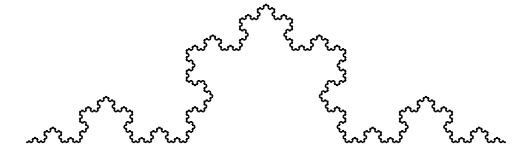
\includegraphics[width=0.7\linewidth]{images/chapter_5_2.png} % Ajusta el nombre del archivo
\caption{Una curva de Koch.}
\label{fig:koch}
\end{figure}


\begin{lstlisting}
def draw(t, length, n):
    if n == 0:
        return
    angle = 50
    t.fd(length*n)
    t.lt(angle)
    draw(t, length, n-1)
    t.rt(2*angle)
    draw(t, length, n-1)
    t.lt(angle)
    t.bk(length*n)
\end{lstlisting}

\textbf{Ejercicio 5.6.} La curva de Koch es un fractal que se parece algo a la Figura~\ref{fig:koch}. Para dibujar una curva de Koch con longitud $x$, todo lo que tienes que hacer es

\begin{enumerate}
\item Dibujar una curva de Koch con longitud $x/3$.
\item Girar a la izquierda 60 grados.
\item Dibujar una curva de Koch con longitud $x/3$.
\item Girar a la derecha 120 grados.
\item Dibujar una curva de Koch con longitud $x/3$.
\item Girar a la izquierda 60 grados.
\item Dibujar una curva de Koch con longitud $x/3$.
\end{enumerate}

La excepción es si $x$ es menor que 3: en ese caso, puedes simplemente dibujar una línea recta con longitud $x$.

\begin{enumerate}
\item Escribe una función llamada \texttt{koch} que tome una tortuga y una longitud como parámetros, y que use la tortuga para dibujar una curva de Koch con la longitud dada.

\item Escribe una función llamada \texttt{snowflake} que dibuje tres curvas de Koch para hacer el contorno de un copo de nieve.

Solución: \texttt{https://thinkpython.com/code/koch.py}

\item La curva de Koch puede generalizarse de varias maneras. Ve \texttt{http://en.wikipedia.org/wiki/Koch\_snowflake} para ejemplos e implementa tu fractal favorito.
\end{enumerate}

%Chapter 6
\chapter{Funciones productivas}

Muchas de las funciones de Python que hemos utilizado, como las funciones matemáticas, producen valores de retorno. Pero las funciones que hemos escrito son todas nulas: tienen un efecto, como imprimir un valor o mover una tortuga, pero no tienen un valor de retorno. En este capítulo aprenderás a escribir funciones productivas.

\section{Valores de retorno}

Llamar a la función genera un valor de retorno, que normalmente asignamos a una variable o usamos como parte de una expresión.

\begin{lstlisting}[language=Python]
e = math.exp(1.0)
height = radius * math.sin(radians)
\end{lstlisting}

Las funciones que hemos escrito hasta ahora son nulas. Hablando informalmente, no tienen valor de retorno; más precisamente, su valor de retorno es \texttt{None}.

En este capítulo, vamos (finalmente) a escribir funciones productivas. El primer ejemplo es \texttt{area}, que devuelve el área de un círculo con el radio dado:

\begin{lstlisting}[language=Python]
def area(radius):
    a = math.pi * radius**2
    return a
\end{lstlisting}

Hemos visto la sentencia \texttt{return} antes, pero en una función productiva la sentencia \texttt{return} incluye una expresión. Esta sentencia significa: "Retorna inmediatamente de esta función y usa la siguiente expresión como valor de retorno". La expresión puede ser arbitrariamente complicada, así que podríamos haber escrito esta función de manera más concisa:

\begin{lstlisting}[language=Python]
def area(radius):
    return math.pi * radius**2
\end{lstlisting}

Por otro lado, las \textbf{variables temporales} como \texttt{a} pueden facilitar la depuración.

A veces es útil tener múltiples sentencias \texttt{return}, una en cada rama de un condicional:

\begin{lstlisting}[language=Python]
def absolute_value(x):
    if x < 0:
        return -x
    else:
        return x
\end{lstlisting}

Como estas sentencias \texttt{return} están en un condicional alternativo, solo una se ejecuta.

Tan pronto como se ejecuta una sentencia \texttt{return}, la función termina sin ejecutar ninguna sentencia posterior. El código que aparece después de una sentencia \texttt{return}, o cualquier otro lugar al que el flujo de ejecución nunca pueda llegar, se llama \textbf{código muerto}.

En una función productiva, es una buena idea asegurarse de que cada posible camino a través del programa llegue a una sentencia \texttt{return}. Por ejemplo:

\begin{lstlisting}[language=Python]
def absolute_value(x):
    if x < 0:
        return -x
    if x > 0:
        return x
\end{lstlisting}

Esta función es incorrecta porque si \texttt{x} es 0, ninguna condición es verdadera y la función termina sin llegar a una sentencia \texttt{return}. Si el flujo de ejecución llega al final de una función, el valor de retorno es \texttt{None}, que no es el valor absoluto de 0.

\begin{lstlisting}[language=Python]
>>> print(absolute_value(0))
None
\end{lstlisting}

Por cierto, Python proporciona una función incorporada llamada \texttt{abs} que calcula valores absolutos.

Como ejercicio, escribe una función \texttt{compare} que tome dos valores, \texttt{x} e \texttt{y}, y devuelva 1 si \texttt{x > y}, 0 si \texttt{x == y}, y -1 si \texttt{x < y}.

\section{Desarrollo incremental}

A medida que escribes funciones más grandes, podrías encontrarte pasando más tiempo depurando.

Para manejar programas cada vez más complejos, es posible que desees probar un proceso llamado \textbf{desarrollo incremental}. El objetivo del desarrollo incremental es evitar largas sesiones de depuración agregando y probando solo una pequeña cantidad de código a la vez.

Como ejemplo, supongamos que deseas encontrar la distancia entre dos puntos, dados por las coordenadas $(x_1, y_1)$ y $(x_2, y_2)$. Por el teorema de Pitágoras, la distancia es:

\[
\text{distancia} = \sqrt{(x_2 - x_1)^2 + (y_2 - y_1)^2}
\]

El primer paso es considerar cómo debería verse una función \texttt{distance} en Python. En otras palabras, ¿cuáles son las entradas (parámetros) y cuál es la salida (valor de retorno)?

En este caso, las entradas son dos puntos, que puedes representar usando cuatro números. El valor de retorno es la distancia representada por un valor de punto flotante.

Inmediatamente puedes escribir un esquema de la función:

\begin{lstlisting}[language=Python]
def distance(x1, y1, x2, y2):
    return 0.0
\end{lstlisting}

Obviamente, esta versión no calcula distancias; siempre devuelve cero. Pero es sintácticamente correcta y se ejecuta, lo que significa que puedes probarla antes de hacerla más complicada.

Para probar la nueva función, llámala con argumentos de muestra:

\begin{lstlisting}[language=Python]
>>> distance(1, 2, 4, 6)
0.0
\end{lstlisting}

Elegí estos valores para que la distancia horizontal sea 3 y la distancia vertical sea 4; de esa manera, el resultado es 5, la hipotenusa de un triángulo rectángulo 3-4-5. Al probar una función, es útil conocer la respuesta correcta.

En este punto hemos confirmado que la función es sintácticamente correcta y podemos comenzar a agregar código al cuerpo. Un siguiente paso razonable es encontrar las diferencias $x_2 - x_1$ y $y_2 - y_1$. La siguiente versión almacena esos valores en variables temporales y los imprime.

\begin{lstlisting}[language=Python]
def distance(x1, y1, x2, y2):
    dx = x2 - x1
    dy = y2 - y1
    print('dx is', dx)
    print('dy is', dy)
    return 0.0
\end{lstlisting}

Si la función está funcionando, debería mostrar \texttt{dx is 3} y \texttt{dy is 4}. Si es así, sabemos que la función está recibiendo los argumentos correctos y realizando el primer cálculo correctamente. Si no, solo hay unas pocas líneas para revisar.

Luego calculamos la suma de los cuadrados de \texttt{dx} y \texttt{dy}:

\begin{lstlisting}[language=Python]
def distance(x1, y1, x2, y2):
    dx = x2 - x1
    dy = y2 - y1
    dsquared = dx**2 + dy**2
    print('dsquared is: ', dsquared)
    return 0.0
\end{lstlisting}

Nuevamente, ejecutarías el programa en esta etapa y verificarías la salida (que debería ser 25). Finalmente, puedes usar \texttt{math.sqrt} para calcular y devolver el resultado:

\begin{lstlisting}[language=Python]
def distance(x1, y1, x2, y2):
    dx = x2 - x1
    dy = y2 - y1
    dsquared = dx**2 + dy**2
    result = math.sqrt(dsquared)
    return result
\end{lstlisting}

Si eso funciona correctamente, has terminado. De lo contrario, podrías imprimir el valor de \texttt{result} antes de la sentencia \texttt{return}.

La versión final de la función no muestra nada cuando se ejecuta; solo devuelve un valor. Las sentencias \texttt{print} que escribimos son útiles para depurar, pero una vez que la función funciona, deberías eliminarlas. Ese tipo de código se llama \textbf{andamiaje} porque es útil para construir el programa pero no es parte del producto final.

Cuando comienzas, solo deberías agregar una o dos líneas de código a la vez. A medida que ganes más experiencia, podrías encontrarte escribiendo y depurando fragmentos más grandes. De cualquier manera, el desarrollo incremental puede ahorrarte mucho tiempo de depuración.

Los aspectos clave del proceso son:

\begin{enumerate}
    \item Comienza con un programa que funcione y haz pequeños cambios incrementales. En cualquier punto, si hay un error, deberías tener una buena idea de dónde está.
    \item Usa variables para contener valores intermedios para que puedas mostrarlos y verificarlos.
    \item Una vez que el programa funcione, podrías eliminar parte del andamiaje o consolidar múltiples sentencias en expresiones compuestas, pero solo si no dificulta la lectura del programa.
\end{enumerate}

Como ejercicio, usa el desarrollo incremental para escribir una función llamada \texttt{hypotenuse} que devuelva la longitud de la hipotenusa de un triángulo rectángulo dados los largos de los otros dos lados como argumentos. Registra cada etapa del proceso de desarrollo a medida que avanzas.

\section{Composición}

Como ya deberías esperar, puedes llamar a una función desde dentro de otra. Como ejemplo, escribiremos una función que tome dos puntos, el centro del círculo y un punto en el perímetro, y calcule el área del círculo.

Supongamos que el punto central está almacenado en las variables \texttt{xc} e \texttt{yc}, y el punto del perímetro está en \texttt{xp} e \texttt{yp}. El primer paso es encontrar el radio del círculo, que es la distancia entre los dos puntos. Acabamos de escribir una función, \texttt{distance}, que hace eso:

\begin{lstlisting}[language=Python]
radius = distance(xc, yc, xp, yp)
\end{lstlisting}

El siguiente paso es encontrar el área de un círculo con ese radio; también acabamos de escribir eso:

\begin{lstlisting}[language=Python]
result = area(radius)
\end{lstlisting}

Encapsulando estos pasos en una función, obtenemos:

\begin{lstlisting}[language=Python]
def circle_area(xc, yc, xp, yp):
    radius = distance(xc, yc, xp, yp)
    result = area(radius)
    return result
\end{lstlisting}

Las variables temporales \texttt{radius} y \texttt{result} son útiles para el desarrollo y la depuración, pero una vez que el programa funciona, podemos hacerlo más conciso componiendo las llamadas a funciones:

\begin{lstlisting}[language=Python]
def circle_area(xc, yc, xp, yp):
    return area(distance(xc, yc, xp, yp))
\end{lstlisting}

\section{Funciones booleanas}

Las funciones pueden devolver booleanos, lo que a menudo es conveniente para ocultar pruebas complicadas dentro de funciones. Por ejemplo:

\begin{lstlisting}[language=Python]
def is_divisible(x, y):
    if x % y == 0:
        return True
    else:
        return False
\end{lstlisting}

Es común dar a las funciones booleanas nombres que suenen como preguntas de sí/no; \texttt{is\_divisible} devuelve \texttt{True} o \texttt{False} para indicar si \texttt{x} es divisible por \texttt{y}.

Aquí hay un ejemplo:

\begin{lstlisting}[language=Python]
>>> is_divisible(6, 4)
False
>>> is_divisible(6, 3)
True
\end{lstlisting}

El resultado del operador \texttt{==} es un booleano, por lo que podemos escribir la función de manera más concisa devolviéndolo directamente:

\begin{lstlisting}[language=Python]
def is_divisible(x, y):
    return x % y == 0
\end{lstlisting}

Las funciones booleanas se usan a menudo en sentencias condicionales:

\begin{lstlisting}[language=Python]
if is_divisible(x, y):
    print('x is divisible by y')
\end{lstlisting}

Podría ser tentador escribir algo como:

\begin{lstlisting}[language=Python]
if is_divisible(x, y) == True:
    print('x is divisible by y')
\end{lstlisting}

Pero la comparación adicional es innecesaria. Como ejercicio, escribe una función \texttt{is\_between(x, y, z)} que devuelva \texttt{True} si $x \leq y \leq z$ o \texttt{False} en caso contrario.

\section{Más recursión}

Hemos cubierto solo un pequeño subconjunto de Python, pero te podría interesar saber que este subconjunto es un lenguaje de programación \textit{completo}, lo que significa que cualquier cosa que se pueda calcular se puede expresar en este lenguaje. Cualquier programa escrito podría reescribirse usando solo las características del lenguaje que has aprendido hasta ahora (en realidad, necesitarías algunos comandos para controlar dispositivos como el mouse, discos, etc., pero eso es todo).

Probar esa afirmación es un ejercicio no trivial realizado por primera vez por Alan Turing, uno de los primeros informáticos (algunos argumentarían que era un matemático, pero muchos de los primeros informáticos comenzaron como matemáticos). En consecuencia, se conoce como la Tesis de Turing. Para una discusión más completa (y precisa) de la Tesis de Turing, recomiendo el libro \textit{Introduction to the Theory of Computation} de Michael Sipser.

Para darte una idea de lo que puedes hacer con las herramientas que has aprendido hasta ahora, evaluaremos algunas funciones matemáticas definidas recursivamente. Una definición recursiva es similar a una definición circular, en el sentido de que la definición contiene una referencia a lo que se está definiendo. Una definición verdaderamente circular no es muy útil:

\textbf{vorpal}: Un adjetivo usado para describir algo que es vorpal.

Si vieras esa definición en el diccionario, podrías molestarte. Por otro lado, si buscaras la definición de la función factorial, denotada con el símbolo !, podrías encontrar algo como esto:

\[
0! = 1
\]
\[
n! = n(n-1)!
\]

Esta definición dice que el factorial de 0 es 1, y el factorial de cualquier otro valor, $n$, es $n$ multiplicado por el factorial de $n-1$.

Entonces 3! es 3 veces 2!, que es 2 veces 1!, que es 1 veces 0!. Juntando todo, 3! es igual a 3 veces 2 veces 1 veces 1, que es 6.

Si puedes escribir una definición recursiva de algo, puedes escribir un programa en Python para evaluarlo. El primer paso es decidir cuáles deberían ser los parámetros. En este caso, está claro que \texttt{factorial} toma un entero:

\begin{lstlisting}[language=Python]
def factorial(n):
\end{lstlisting}

Si el argumento resulta ser 0, todo lo que tenemos que hacer es devolver 1:

\begin{lstlisting}[language=Python]
def factorial(n):
    if n == 0:
        return 1
\end{lstlisting}

De lo contrario, y esta es la parte interesante, tenemos que hacer una llamada recursiva para encontrar el factorial de $n-1$ y luego multiplicarlo por $n$:

\begin{lstlisting}[language=Python]
def factorial(n):
    if n == 0:
        return 1
    else:
        recurse = factorial(n-1)
        result = n * recurse
        return result
\end{lstlisting}

El flujo de ejecución para este programa es similar al flujo de \texttt{countdown} en la Sección 5.8. Si llamamos a \texttt{factorial} con el valor 3:

Como 3 no es 0, tomamos la segunda rama y calculamos el factorial de \texttt{n-1}...

Como 2 no es 0, tomamos la segunda rama y calculamos el factorial de \texttt{n-1}...

Como 1 no es 0, tomamos la segunda rama y calculamos el factorial de \texttt{n-1}...

Como 0 es igual a 0, tomamos la primera rama y devolvemos 1 sin hacer más llamadas recursivas.

El valor de retorno, 1, se multiplica por \texttt{n}, que es 1, y el resultado se devuelve.

El valor de retorno, 1, se multiplica por \texttt{n}, que es 2, y el resultado se devuelve.

El valor de retorno (2) se multiplica por \texttt{n}, que es 3, y el resultado, 6, se convierte en el valor de retorno de la llamada a función que inició todo el proceso.

La Figura 6.1 muestra cómo se ve el diagrama de pila para esta secuencia de llamadas a funciones.

Los valores de retorno se muestran siendo pasados hacia arriba en la pila. En cada marco, el valor de retorno es el valor de \texttt{result}, que es el producto de \texttt{n} y \texttt{recurse}.

En el último marco, las variables locales \texttt{recurse} y \texttt{result} no existen, porque la rama que las crea no se ejecuta.

\begin{figure}[h]
        \centering
        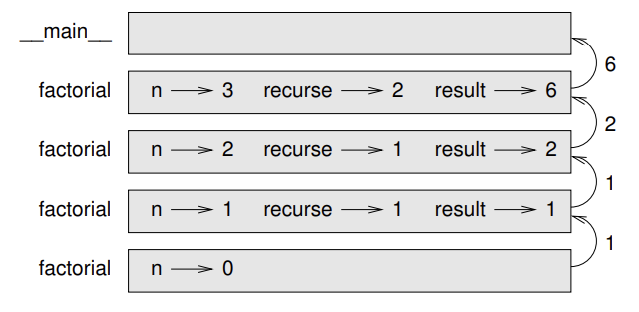
\includegraphics[width=0.5\textwidth]{./images/chapter_6_1.png}
        \caption{Diagrama de Pila.}
        \label{fig:6_1}
        \end{figure}
\section{Salto de fe}

Seguir el flujo de ejecución es una forma de leer programas, pero rápidamente puede volverse abrumador. Una alternativa es lo que yo llamo el "salto de fe". Cuando llegas a una llamada a función, en lugar de seguir el flujo de ejecución, asumes que la función funciona correctamente y devuelve el resultado correcto.

De hecho, ya estás practicando este salto de fe cuando usas funciones incorporadas. Cuando llamas a \texttt{math.cos} o \texttt{math.exp}, no examinas los cuerpos de esas funciones. Simplemente asumes que funcionan porque las personas que escribieron las funciones incorporadas eran buenos programadores.

Lo mismo ocurre cuando llamas a una de tus propias funciones. Por ejemplo, en la Sección 6.4, escribimos una función llamada \texttt{is\_divisible} que determina si un número es divisible por otro. Una vez que nos hemos convencido de que esta función es correcta (examinando el código y probándolo), podemos usar la función sin mirar el cuerpo nuevamente.

Lo mismo ocurre con los programas recursivos. Cuando llegas a la llamada recursiva, en lugar de seguir el flujo de ejecución, deberías asumir que la llamada recursiva funciona (devuelve el resultado correcto) y luego preguntarte: "Asumiendo que puedo encontrar el factorial de $n-1$, ¿puedo calcular el factorial de $n$?" Está claro que puedes, multiplicando por $n$.

Por supuesto, es un poco extraño asumir que la función funciona correctamente cuando no has terminado de escribirla, ¡pero por eso se llama salto de fe!

\section{Un ejemplo más}

Después de \texttt{factorial}, el ejemplo más común de una función matemática definida recursivamente es \texttt{fibonacci}, que tiene la siguiente definición (ver \url{http://en.wikipedia.org/wiki/Fibonacci_number}):

\[
\text{fibonacci}(0) = 0
\]
\[
\text{fibonacci}(1) = 1
\]
\[
\text{fibonacci}(n) = \text{fibonacci}(n-1) + \text{fibonacci}(n-2)
\]

Traducido a Python, se ve así:

\begin{lstlisting}[language=Python]
def fibonacci(n):
    if n == 0:
        return 0
    elif n == 1:
        return 1
    else:
        return fibonacci(n-1) + fibonacci(n-2)
\end{lstlisting}

Si intentas seguir el flujo de ejecución aquí, incluso para valores bastante pequeños de $n$, tu cabeza explotará. Pero según el salto de fe, si asumes que las dos llamadas recursivas funcionan correctamente, entonces está claro que obtienes el resultado correcto sumándolas.

\section{Verificación de tipos}

¿Qué sucede si llamamos a \texttt{factorial} y le damos 1.5 como argumento?

\begin{lstlisting}[language=Python]
>>> factorial(1.5)
RuntimeError: Maximum recursion depth exceeded
\end{lstlisting}

Parece una recursión infinita. ¿Cómo puede ser? La función tiene un caso base: cuando \texttt{n == 0}. Pero si \texttt{n} no es un entero, podemos perder el caso base y recurrir para siempre.

En la primera llamada recursiva, el valor de \texttt{n} es 0.5. En la siguiente, es -0.5. A partir de ahí, se vuelve más pequeño (más negativo), pero nunca será 0.

Tenemos dos opciones. Podemos intentar generalizar la función \texttt{factorial} para que funcione con números de punto flotante, o podemos hacer que \texttt{factorial} verifique el tipo de su argumento. La primera opción se llama función gamma y está un poco más allá del alcance de este libro. Así que optaremos por la segunda.

Podemos usar la función incorporada \texttt{isinstance} para verificar el tipo del argumento. Mientras estamos en eso, también podemos asegurarnos de que el argumento sea positivo:

\begin{lstlisting}[language=Python]
def factorial(n):
    if not isinstance(n, int):
        print('Factorial is only defined for integers.')
        return None
    elif n < 0:
        print('Factorial is not defined for negative integers.')
        return None
    elif n == 0:
        return 1
    else:
        return n * factorial(n-1)
\end{lstlisting}

El primer caso base maneja no enteros; el segundo maneja enteros negativos. En ambos casos, el programa imprime un mensaje de error y devuelve \texttt{None} para indicar que algo salió mal:

\begin{lstlisting}[language=Python]
>>> print(factorial('fred'))
Factorial is only defined for integers.
None
>>> print(factorial(-2))
Factorial is not defined for negative integers.
None
\end{lstlisting}

Si pasamos ambas verificaciones, sabemos que \texttt{n} es un entero no negativo, por lo que podemos probar que la recursión termina.

Este programa demuestra un patrón a veces llamado \textbf{guardián}. Los dos primeros condicionales actúan como guardianes, protegiendo el código que sigue de valores que podrían causar un error. Los guardianes hacen posible probar la corrección del código.

En la Sección 11.4 veremos una alternativa más flexible a imprimir un mensaje de error: generar una excepción.

\section{Depuración}

Dividir un programa grande en funciones más pequeñas crea puntos de control naturales para la depuración. Si una función no funciona, hay tres posibilidades a considerar:

\begin{itemize}
    \item Hay algo mal con los argumentos que recibe la función; se viola una precondición.
    \item Hay algo mal con la función; se viola una postcondición.
    \item Hay algo mal con el valor de retorno o la forma en que se está utilizando.
\end{itemize}

Para descartar la primera posibilidad, puedes agregar una sentencia \texttt{print} al principio de la función y mostrar los valores de los parámetros (y tal vez sus tipos). O puedes escribir código que verifique las precondiciones explícitamente.

Si los parámetros parecen buenos, agrega una sentencia \texttt{print} antes de cada sentencia \texttt{return} y muestra el valor de retorno. Si es posible, verifica el resultado manualmente. Considera llamar a la función con valores que faciliten la verificación del resultado (como en la Sección 6.2).

Si la función parece estar funcionando, mira la llamada a función para asegurarte de que el valor de retorno se esté usando correctamente (¡o que se esté usando!).

Agregar sentencias \texttt{print} al principio y al final de una función puede ayudar a hacer más visible el flujo de ejecución. Por ejemplo, aquí hay una versión de \texttt{factorial} con sentencias \texttt{print}:

\begin{lstlisting}[language=Python]
def factorial(n):
    space = ' ' * (4 * n)
    print(space, 'factorial', n)
    if n == 0:
        print(space, 'returning 1')
        return 1
    else:
        recurse = factorial(n-1)
        result = n * recurse
        print(space, 'returning', result)
        return result
\end{lstlisting}

\texttt{space} es una cadena de caracteres de espacio que controla la sangría de la salida. Aquí está el resultado de \texttt{factorial(4)}:

\begin{lstlisting}[language=Python]
factorial 4
    factorial 3
        factorial 2
            factorial 1
                factorial 0
                returning 1
            returning 1
        returning 2
    returning 6
returning 24
\end{lstlisting}

Si estás confundido acerca del flujo de ejecución, este tipo de salida puede ser útil. Se necesita algo de tiempo para desarrollar andamiaje efectivo, pero un poco de andamiaje puede ahorrar mucha depuración.

\section{Glosario}

\begin{description}
    \item[variable temporal:] Una variable utilizada para almacenar un valor intermedio en un cálculo complejo.
    \item[código muerto:] Parte de un programa que nunca se ejecuta, a menudo porque aparece después de una sentencia \texttt{return}.
    \item[desarrollo incremental:] Un plan de desarrollo de programas destinado a evitar la depuración agregando y probando solo una pequeña cantidad de código a la vez.
    \item[andamiaje:] Código que se usa durante el desarrollo del programa pero que no es parte de la versión final.
    \item[guardián:] Un patrón de programación que usa una sentencia condicional para verificar y manejar circunstancias que podrían causar un error.
\end{description}

\section{Ejercicios}

\textbf{Ejercicio 6.1.} Dibuja un diagrama de pila para el siguiente programa. ¿Qué imprime el programa?

\begin{lstlisting}[language=Python]
def b(z):
    prod = a(z, z)
    print(z, prod)
    return prod

def a(x, y):
    x = x + 1
    return x * y

def c(x, y, z):
    total = x + y + z
    square = b(total)**2
    return square

x = 1
y = x + 1
print(c(x, y+3, x+y))
\end{lstlisting}

\textbf{Ejercicio 6.2.} La función de Ackermann, $A(m, n)$, se define:

\[
A(m, n) =\begin{cases}n+1&\text{si }m=0\\A(m-1,1)&\text{si }m>0\text{ y }n=0\\A(m-1,A(m,n-1))&\text{si }m>0\text{ y }n>0.\end{cases}
\]

Ver \url{http://en.wikipedia.org/wiki/Ackermann_function}. Escribe una función llamada \texttt{ack} que evalúe la función de Ackermann. Usa tu función para evaluar \texttt{ack(3, 4)}, que debería ser 125. ¿Qué sucede para valores mayores de \texttt{m} y \texttt{n}? Solución: \url{https://thinkpython.com/code/ackermann.py}.

\textbf{Ejercicio 6.3.} Un palíndromo es una palabra que se escribe igual al derecho y al revés, como "noon" y "redivider". Recursivamente, una palabra es un palíndromo si la primera y la última letra son iguales y el medio es un palíndromo.

Las siguientes son funciones que toman un argumento de cadena y devuelven la primera, la última y las letras del medio:

\begin{lstlisting}[language=Python]
def first(word):
    return word[0]

def last(word):
    return word[-1]

def middle(word):
    return word[1:-1]
\end{lstlisting}

Veremos cómo funcionan en el Capítulo 8.

\begin{enumerate}
    \item Escribe estas funciones en un archivo llamado \texttt{palindrome.py} y pruébalas. ¿Qué sucede si llamas a \texttt{middle} con una cadena de dos letras? ¿Una letra? ¿Qué pasa con la cadena vacía, que se escribe \texttt{''} y no contiene letras?
    \item Escribe una función llamada \texttt{is\_palindrome} que tome un argumento de cadena y devuelva \texttt{True} si es un palíndromo y \texttt{False} en caso contrario. Recuerda que puedes usar la función incorporada \texttt{len} para verificar la longitud de una cadena.
\end{enumerate}

Solución: \url{https://thinkpython.com/code/palindrome_soln.py}.

\textbf{Ejercicio 6.4.} Un número, \texttt{a}, es una potencia de \texttt{b} si es divisible por \texttt{b} y \texttt{a/b} es una potencia de \texttt{b}. Escribe una función llamada \texttt{is\_power} que tome los parámetros \texttt{a} y \texttt{b} y devuelva \texttt{True} si \texttt{a} es una potencia de \texttt{b}. Nota: tendrás que pensar en el caso base.

\textbf{Ejercicio 6.5.} El máximo común divisor (MCD) de \texttt{a} y \texttt{b} es el número más grande que divide a ambos sin dejar resto.

Una forma de encontrar el MCD de dos números se basa en la observación de que si \texttt{r} es el resto cuando \texttt{a} se divide por \texttt{b}, entonces $\text{mcd}(a,b) = \text{mcd}(b,r)$. Como caso base, podemos usar $\text{mcd}(a,0) = a$.

Escribe una función llamada \texttt{gcd} que tome los parámetros \texttt{a} y \texttt{b} y devuelva su máximo común divisor.

Crédito: Este ejercicio está basado en un ejemplo de \textit{Structure and Interpretation of Computer Programs} de Abelson y Sussman.
\chapter{Iteración}

Este capítulo trata sobre la iteración, que es la capacidad de ejecutar un bloque de declaraciones repetidamente. Vimos un tipo de iteración, usando recursión, en la Sección 5.8. Vimos otro tipo, usando un bucle \texttt{for}, en la Sección 4.2. En este capítulo veremos otro tipo más, usando una declaración \texttt{while}. Pero primero quiero decir un poco más sobre la asignación de variables.

\section{Reasignación}

Como puedes haber descubierto, es legal hacer más de una asignación a la misma variable. Una nueva asignación hace que una variable existente se refiera a un nuevo valor (y deje de referirse al valor anterior).

\begin{lstlisting}
>>> x = 5
>>> x
5
>>> x = 7
>>> x
7
\end{lstlisting}

La primera vez que mostramos \texttt{x}, su valor es 5; la segunda vez, su valor es 7.

La Figura~\ref{fig:reassignment} muestra cómo se ve la \textbf{reasignación} en un diagrama de estado.


En este punto quiero abordar una fuente común de confusión. Dado que Python usa el signo igual (\texttt{=}) para la asignación, es tentador interpretar una declaración como \texttt{a = b} como una proposición matemática de igualdad; es decir, la afirmación de que $a$ y $b$ son iguales. Pero esta interpretación es incorrecta.

Primero, la igualdad es una relación simétrica y la asignación no lo es. Por ejemplo, en matemáticas, si $a = 7$ entonces $7 = a$. Pero en Python, la declaración \texttt{a = 7} es legal y \texttt{7 = a} no lo es.

Además, en matemáticas, una proposición de igualdad es verdadera o falsa en todo momento. Si $a = b$ ahora, entonces $a$ siempre será igual a $b$. En Python, una declaración de asignación puede hacer que dos variables sean iguales, pero no tienen que permanecer así:

\begin{figure}[h]
\centering
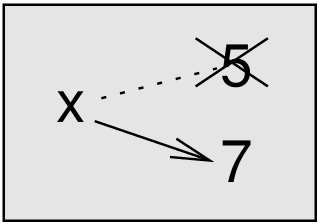
\includegraphics[width=0.7\linewidth]{images/chapter_7_1.png} % Ajusta el nombre del archivo
\caption{Diagrama de estado.}
\label{fig:diagrama_estado}
\end{figure}

\begin{lstlisting}
>>> a = 5
>>> b = a    # a and b are now equal
>>> a = 3    # a and b are no longer equal
>>> b
5
\end{lstlisting}

La tercera línea cambia el valor de \texttt{a} pero no cambia el valor de \texttt{b}, por lo que ya no son iguales.

Reasignar variables es a menudo útil, pero debes usarlo con precaución. Si los valores de las variables cambian frecuentemente, puede hacer que el código sea difícil de leer y depurar.

\section{Actualización de variables}

Un tipo común de reasignación es una \textbf{actualización}, donde el nuevo valor de la variable depende del anterior.

\begin{lstlisting}
>>> x = x + 1
\end{lstlisting}

Esto significa ``obtener el valor actual de \texttt{x}, agregar uno, y luego actualizar \texttt{x} con el nuevo valor.''

Si intentas actualizar una variable que no existe, obtienes un error, porque Python evalúa el lado derecho antes de asignar un valor a \texttt{x}:

\begin{lstlisting}
>>> x = x + 1
NameError: name 'x' is not defined
\end{lstlisting}

Antes de que puedas actualizar una variable, tienes que \textbf{inicializarla}, generalmente con una asignación simple:

\begin{lstlisting}
>>> x = 0
>>> x = x + 1
\end{lstlisting}

Actualizar una variable agregando 1 se llama un \textbf{incremento}; restar 1 se llama un \textbf{decremento}.

\section{La declaración \texttt{while}}

Las computadoras se usan a menudo para automatizar tareas repetitivas. Repetir tareas idénticas o similares sin cometer errores es algo que las computadoras hacen bien y las personas hacen mal. En un programa de computadora, la repetición también se llama \textbf{iteración}.

Ya hemos visto dos funciones, \texttt{countdown} y \texttt{print\_n}, que iteran usando recursión. Debido a que la iteración es tan común, Python proporciona características del lenguaje para hacerla más fácil. Una es la declaración \texttt{for} que vimos en la Sección 4.2. Volveremos a eso más tarde.

Otra es la declaración \texttt{while}. Aquí hay una versión de \texttt{countdown} que usa una declaración \texttt{while}:

\begin{lstlisting}
def countdown(n):
    while n > 0:
        print(n)
        n = n - 1
    print('Blastoff!')
\end{lstlisting}

Casi puedes leer la declaración \texttt{while} como si fuera inglés. Significa, ``Mientras \texttt{n} sea mayor que 0, muestra el valor de \texttt{n} y luego decrementa \texttt{n}. Cuando llegues a 0, muestra la palabra \texttt{Blastoff!}''

Más formalmente, aquí está el flujo de ejecución para una declaración \texttt{while}:

\begin{enumerate}
\item Determinar si la condición es verdadera o falsa.
\item Si es falsa, salir de la declaración \texttt{while} y continuar la ejecución en la siguiente declaración.
\item Si la condición es verdadera, ejecutar el cuerpo y luego volver al paso 1.
\end{enumerate}

Este tipo de flujo se llama un bucle porque el tercer paso se repite hacia el principio.

El cuerpo del bucle debe cambiar el valor de una o más variables para que la condición se vuelva falsa eventualmente y el bucle termine. De lo contrario, el bucle se repetirá para siempre, lo que se llama un \textbf{bucle infinito}. Una fuente inagotable de diversión para los científicos de la computación es la observación de que las instrucciones en el champú, ``Enjabonar, enjuagar, repetir'', son un bucle infinito.

En el caso de \texttt{countdown}, podemos probar que el bucle termina: si \texttt{n} es cero o negativo, el bucle nunca se ejecuta. De lo contrario, \texttt{n} se vuelve más pequeño cada vez a través del bucle, por lo que eventualmente tenemos que llegar a 0.

Para algunos otros bucles, no es tan fácil de decir. Por ejemplo:

\begin{lstlisting}
def sequence(n):
    while n != 1:
        print(n)
        if n % 2 == 0:        # n is even
            n = n / 2
        else:                 # n is odd
            n = n*3 + 1
\end{lstlisting}

La condición para este bucle es \texttt{n != 1}, por lo que el bucle continuará hasta que \texttt{n} sea 1, lo que hace que la condición sea falsa.

Cada vez a través del bucle, el programa muestra el valor de \texttt{n} y luego verifica si es par o impar. Si es par, \texttt{n} se divide por 2. Si es impar, el valor de \texttt{n} se reemplaza con \texttt{n*3 + 1}. Por ejemplo, si el argumento pasado a \texttt{sequence} es 3, los valores resultantes de \texttt{n} son 3, 10, 5, 16, 8, 4, 2, 1.

Dado que \texttt{n} a veces aumenta y a veces disminuye, no hay una prueba obvia de que \texttt{n} alguna vez llegue a 1, o que el programa termine. Para algunos valores particulares de \texttt{n}, podemos probar la terminación. Por ejemplo, si el valor inicial es una potencia de dos, \texttt{n} será par cada vez a través del bucle hasta que llegue a 1. El ejemplo anterior termina con una secuencia de este tipo, comenzando con 16.

La pregunta difícil es si podemos probar que este programa termina para \emph{todos} los valores positivos de \texttt{n}. Hasta ahora, nadie ha podido probarlo o refutarlo. (Ver \texttt{http://en.wikipedia.org/wiki/Collatz\_conjecture}.)

Como ejercicio, reescribe la función \texttt{print\_n} de la Sección 5.8 usando iteración en lugar de recursión.

\section{\texttt{break}}

A veces no sabes que es hora de terminar un bucle hasta que llegas a la mitad del cuerpo. En ese caso puedes usar la declaración \texttt{break} para saltar fuera del bucle.

Por ejemplo, supón que quieres recibir entrada del usuario hasta que escriban \texttt{done}. Podrías escribir:

\begin{lstlisting}
while True:
    line = input('> ')
    if line == 'done':
        break
    print(line)

print('Done!')
\end{lstlisting}

La condición del bucle es \texttt{True}, que siempre es verdadera, por lo que el bucle se ejecuta hasta que toca la declaración \texttt{break}.

Cada vez que pasa, solicita al usuario con un corchete angular. Si el usuario escribe \texttt{done}, la declaración \texttt{break} sale del bucle. De lo contrario, el programa repite lo que sea que el usuario escriba y vuelve al principio del bucle. Aquí hay una ejecución de muestra:

\begin{lstlisting}
> not done
not done
> done
Done!
\end{lstlisting}

Esta forma de escribir bucles \texttt{while} es común porque puedes verificar la condición en cualquier lugar del bucle (no solo al principio) y puedes expresar la condición de parada afirmativamente (``parar cuando esto suceda'') en lugar de negativamente (``seguir hasta que eso suceda'').

\subsection{Raíces cuadradas}

Los bucles se usan a menudo en programas que calculan resultados numéricos comenzando con una respuesta aproximada y mejorándola iterativamente.

Por ejemplo, una forma de calcular raíces cuadradas es el método de Newton. Supón que quieres conocer la raíz cuadrada de $a$. Si comienzas con casi cualquier estimación, $x$, puedes calcular una mejor estimación con la siguiente fórmula:

$$y = \frac{x + a/x}{2}$$

Por ejemplo, si $a$ es 4 y $x$ es 3:

\begin{lstlisting}
>>> a = 4
>>> x = 3
>>> y = (x + a/x) / 2
>>> y
2.1666666667
\end{lstlisting}

El resultado está más cerca de la respuesta correcta ($\sqrt{4} = 2$). Si repetimos el proceso con la nueva estimación, se acerca aún más:

\begin{lstlisting}
>>> x = y
>>> y = (x + a/x) / 2
>>> y
2.0064102564
\end{lstlisting}

Después de unas pocas actualizaciones más, la estimación es casi exacta:

\begin{lstlisting}
>>> x = y
>>> y = (x + a/x) / 2
>>> y
2.0001024003
>>> x = y
>>> y = (x + a/x) / 2
>>> y
2.0000000003
\end{lstlisting}

En general, no sabemos de antemano cuántos pasos toma llegar a la respuesta correcta, pero sabemos cuándo llegamos allí porque la estimación deja de cambiar:

\begin{lstlisting}
>>> x = y
>>> y = (x + a/x) / 2
>>> y
2.0
>>> x = y
>>> y = (x + a/x) / 2
>>> y
2.0
\end{lstlisting}

Cuando $y == x$, podemos parar. Aquí hay un bucle que comienza con una estimación inicial, $x$, y la mejora hasta que deja de cambiar:

\begin{lstlisting}
while True:
    print(x)
    y = (x + a/x) / 2
    if y == x:
        break
    x = y
\end{lstlisting}

Para la mayoría de los valores de $a$ esto funciona bien, pero en general es peligroso probar la igualdad de \texttt{float}. Los valores de punto flotante son solo aproximadamente correctos: la mayoría de los números racionales, como $1/3$, y los números irracionales, como $\sqrt{2}$, no se pueden representar exactamente con un \texttt{float}.

En lugar de verificar si $x$ y $y$ son exactamente iguales, es más seguro usar la función incorporada \texttt{abs} para calcular el valor absoluto, o magnitud, de la diferencia entre ellos:

\begin{lstlisting}
if abs(y-x) < epsilon:
    break
\end{lstlisting}

Donde \texttt{epsilon} tiene un valor como \texttt{0.0000001} que determina qué tan cerca es lo suficientemente cerca.

\section{Algoritmos}

El método de Newton es un ejemplo de un \textbf{algoritmo}: es un proceso mecánico para resolver una categoría de problemas (en este caso, calcular raíces cuadradas).

Para entender qué es un algoritmo, podría ayudar comenzar con algo que no es un algoritmo. Cuando aprendiste a multiplicar números de un solo dígito, probablemente memorizaste la tabla de multiplicación. En efecto, memorizaste 100 soluciones específicas. Ese tipo de conocimiento no es algorítmico.

Pero si fueras ``perezoso'', podrías haber aprendido algunos trucos. Por ejemplo, para encontrar el producto de $n$ y 9, puedes escribir $n - 1$ como el primer dígito y $10 - n$ como el segundo dígito. Este truco es una solución general para multiplicar cualquier número de un solo dígito por 9. ¡Eso es un algoritmo!

De manera similar, las técnicas que aprendiste para la suma con llevar, la resta con préstamo, y la división larga son todos algoritmos. Una de las características de los algoritmos es que no requieren ninguna inteligencia para ejecutarlos. Son procesos mecánicos donde cada paso sigue del último de acuerdo con un conjunto simple de reglas.

Ejecutar algoritmos es aburrido, pero diseñarlos es interesante, intelectualmente desafiante, y una parte central de la informática.

Algunas de las cosas que la gente hace naturalmente, sin dificultad o pensamiento consciente, son las más difíciles de expresar algorítmicamente. Entender el lenguaje natural es un buen ejemplo. Todos lo hacemos, pero hasta ahora nadie ha sido capaz de explicar \emph{cómo} lo hacemos, al menos no en la forma de un algoritmo.

\section{Depuración}

A medida que comiences a escribir programas más grandes, podrías encontrarte pasando más tiempo depurando. Más código significa más oportunidades de cometer errores y más lugares donde los bugs pueden esconderse.

Una forma de reducir tu tiempo de depuración es la ``depuración por bisección''. Por ejemplo, si hay 100 líneas en tu programa y las revisas una por una, tomaría 100 pasos.

En su lugar, trata de dividir el problema por la mitad. Busca el medio del programa, o cerca de él, un valor intermedio que puedas verificar. Agrega una declaración \texttt{print} (o algo más que tenga un efecto verificable) y ejecuta el programa.

Si la verificación del punto medio es incorrecta, debe haber un problema en la primera mitad del programa. Si es correcta, el problema está en la segunda mitad.

Cada vez que realizas una verificación como esta, reduces a la mitad el número de líneas que tienes que buscar. Después de seis pasos (que es menos de 100), estarías reducido a una o dos líneas de código, al menos en teoría.

En la práctica, no siempre está claro qué es el ``medio del programa'' y no siempre es posible verificarlo. No tiene sentido contar líneas y encontrar el punto medio exacto. En su lugar, piensa en lugares del programa donde podría haber errores y lugares donde es fácil poner una verificación. Luego elige un punto que divida el espacio de búsqueda aproximadamente por la mitad, ya sea que el bug esté antes o después de la verificación.

\section{Glosario}

\textbf{reasignación:} Asignar un nuevo valor a una variable que ya existe.

\textbf{actualización:} Una asignación donde el nuevo valor de la variable depende del valor anterior.

\textbf{inicialización:} Una asignación que da un valor inicial a una variable que será actualizada.

\textbf{incremento:} Una actualización que aumenta el valor de una variable (a menudo en uno).

\textbf{decremento:} Una actualización que disminuye el valor de una variable.

\textbf{iteración:} Ejecución repetida de un conjunto de declaraciones usando ya sea una llamada de función recursiva o un bucle.

\textbf{bucle infinito:} Un bucle en el cual la condición de terminación nunca se satisface.

\textbf{algoritmo:} Un proceso general para resolver una categoría de problemas.

\section{Ejercicios}

\textbf{Ejercicio 7.1.} Copia el bucle de la Sección 7.3 y encapsúlalo en una función llamada \texttt{mysqrt} que toma \texttt{a} como parámetro, elige un valor razonable de \texttt{x}, y devuelve una estimación de la raíz cuadrada de \texttt{a}.

Para probarlo, escribe una función llamada \texttt{test\_square\_root} que imprima una tabla como esta:

\begin{lstlisting}
a    mysqrt(a)     math.sqrt(a)  diff
-    ---------     ------------  ----
1.0  1.0           1.0           0.0
2.0  1.41421356237 1.41421356237 2.22044604925e-16
3.0  1.73205080757 1.73205080757 0.0
4.0  2.0           2.0           0.0
5.0  2.23606797775 2.23606797775 0.0
6.0  2.44948974278 2.44948974278 0.0
7.0  2.6457513110  2.6457513110  0.0
8.0  2.82842712475 2.82842712475 4.4408920985e-16
9.0  3.0           3.0           0.0
\end{lstlisting}

La primera columna es un número, \texttt{a}; la segunda columna es la raíz cuadrada de \texttt{a} calculada con \texttt{mysqrt}; la tercera columna es la raíz cuadrada calculada por \texttt{math.sqrt}; la cuarta columna es el valor absoluto de la diferencia entre las dos estimaciones.

\textbf{Ejercicio 7.2.} La función incorporada \texttt{eval} toma una cadena y la evalúa usando el intérprete de Python. Por ejemplo:

\begin{lstlisting}
>>> eval('1 + 2 * 3')
7
>>> import math
>>> eval('math.sqrt(5)')
2.2360679774997898
>>> eval('type(math.pi)')
<class 'float'>
\end{lstlisting}

Escribe una función llamada \texttt{eval\_loop} que iterativamente solicite al usuario, tome la entrada resultante y la evalúe usando \texttt{eval}, e imprima el resultado.

Debe continuar hasta que el usuario ingrese \texttt{'done'}, y luego devolver el valor de la última expresión que evaluó.

\vspace{1cm}

\textbf{Ejercicio 7.3.} El matemático Srinivasa Ramanujan encontró una serie infinita que puede ser usada para generar una aproximación numérica de $1/\pi$:

\begin{equation}
\frac{1}{\pi} = \frac{2\sqrt{2}}{9801} \sum_{k=0}^{\infty} \frac{(4k)!(1103+26390k)}{(k!)^4 396^{4k}}
\end{equation}

Escribe una función llamada \texttt{estimate\_pi} que use esta fórmula para calcular y devolver una estimación de $\pi$. Debe usar un bucle \texttt{while} para calcular términos de la sumatoria hasta que el último término sea menor que \texttt{1e-15} (que es la notación de Python para $10^{-15}$). Puedes verificar el resultado comparándolo con \texttt{math.pi}.

Solución: \texttt{https://thinkpython.com/code/pi.py}
%Chapter 8

\chapter{Cadenas}

Las cadenas no son como enteros, flotantes y booleanos. Una cadena es una \textbf{secuencia}, lo que significa que es una colección ordenada de otros valores. En este capítulo verás cómo acceder a los caracteres que componen una cadena y aprenderás sobre algunos de los métodos que proporcionan las cadenas.

\section{Una cadena es una secuencia}

Una cadena es una secuencia de caracteres. Puedes acceder a los caracteres uno por uno con el operador de corchetes:

\begin{lstlisting}[language=Python]
>>> fruit = 'banana'
>>> letter = fruit[1]
\end{lstlisting}

La segunda sentencia selecciona el carácter número 1 de \texttt{fruit} y lo asigna a \texttt{letter}.

La expresión entre corchetes se llama \textbf{índice}. El índice indica qué carácter de la secuencia deseas (de ahí el nombre).

Pero podrías no obtener lo que esperas:

\begin{lstlisting}[language=Python]
>>> letter
'a'
\end{lstlisting}

Para la mayoría de las personas, la primera letra de 'banana' es b, no a. Pero para los informáticos, el índice es un desplazamiento desde el inicio de la cadena, y el desplazamiento de la primera letra es cero.

\begin{lstlisting}[language=Python]
>>> letter = fruit[0]
>>> letter
'b'
\end{lstlisting}

Entonces, b es la letra 0 ("cero-ésima") de 'banana', a es la letra 1 ("uno-ésima"), y n es la letra 2 ("dos-ésima").

Como índice, puedes usar una expresión que contenga variables y operadores:

\begin{lstlisting}[language=Python]
>>> i = 1
>>> fruit[i]
'a'
>>> fruit[i+1]
'n'
\end{lstlisting}

Pero el valor del índice debe ser un entero. De lo contrario, obtendrás:

\begin{lstlisting}[language=Python]
>>> letter = fruit[1.5]
TypeError: string indices must be integers
\end{lstlisting}

\section{len}

\texttt{len} es una función incorporada que devuelve el número de caracteres en una cadena:

\begin{lstlisting}[language=Python]
>>> fruit = 'banana'
>>> len(fruit)
6
\end{lstlisting}

Para obtener la última letra de una cadena, podrías sentirte tentado a probar algo como esto:

\begin{lstlisting}[language=Python]
>>> length = len(fruit)
>>> last = fruit[length]
IndexError: string index out of range
\end{lstlisting}

La razón del \texttt{IndexError} es que no hay ninguna letra en 'banana' con el índice 6. Como comenzamos a contar desde cero, las seis letras están numeradas del 0 al 5. Para obtener el último carácter, debes restar 1 a \texttt{length}:

\begin{lstlisting}[language=Python]
>>> last = fruit[length-1]
>>> last
'a'
\end{lstlisting}

O puedes usar índices negativos, que cuentan hacia atrás desde el final de la cadena. La expresión \texttt{fruit[-1]} devuelve la última letra, \texttt{fruit[-2]} devuelve la penúltima, y así sucesivamente.

\section{Recorrido con un bucle for}

Muchos cálculos implican procesar una cadena un carácter a la vez. A menudo comienzan al principio, seleccionan cada carácter en turno, hacen algo con él y continúan hasta el final. Este patrón de procesamiento se llama \textbf{recorrido}. Una forma de escribir un recorrido es con un bucle \texttt{while}:

\begin{lstlisting}[language=Python]
index = 0
while index < len(fruit):
    letter = fruit[index]
    print(letter)
    index = index + 1
\end{lstlisting}

Este bucle recorre la cadena y muestra cada letra en una línea por sí misma. La condición del bucle es \texttt{index < len(fruit)}, por lo que cuando \texttt{index} es igual a la longitud de la cadena, la condición es falsa y el cuerpo del bucle no se ejecuta. El último carácter accedido es el que tiene el índice \texttt{len(fruit)-1}, que es el último carácter de la cadena.

Como ejercicio, escribe una función que tome una cadena como argumento y muestre las letras al revés, una por línea.

Otra forma de escribir un recorrido es con un bucle \texttt{for}:

\begin{lstlisting}[language=Python]
for letter in fruit:
    print(letter)
\end{lstlisting}

\begin{figure}[h]
        \centering
        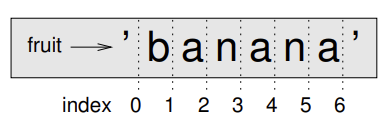
\includegraphics[width=0.5\textwidth]{./images/chapter_8_1.png}
        \caption{Slice Indices.}
        \label{fig:8_1}
        \end{figure}
Cada vez que se ejecuta el bucle, el siguiente carácter de la cadena se asigna a la variable \texttt{letter}. El bucle continúa hasta que no quedan caracteres.

El siguiente ejemplo muestra cómo usar la concatenación (suma de cadenas) y un bucle \texttt{for} para generar una serie abecedaria (es decir, en orden alfabético). En el libro \textit{Make Way for Ducklings} de Robert McCloskey, los nombres de los patitos son Jack, Kack, Lack, Mack, Nack, Quack, Pack y Quack. Este bucle imprime estos nombres en orden:

\begin{lstlisting}[language=Python]
prefixes = 'JKLMNOPQ'
suffix = 'ack'

for letter in prefixes:
    print(letter + suffix)
\end{lstlisting}

La salida es:

\begin{lstlisting}[language=Python]
Jack
Kack
Lack
Mack
Nack
Oack
Pack
Qack
\end{lstlisting}

Por supuesto, eso no es del todo correcto porque "Quack" y "Quack" están mal escritos. Como ejercicio, modifica el programa para corregir este error.

\section{Segmentos de cadena}

Un segmento de una cadena se llama \textbf{slice}. Seleccionar un slice es similar a seleccionar un carácter:

\begin{lstlisting}[language=Python]
>>> s = 'Monty Python'
>>> s[0:5]
'Monty'
>>> s[6:12]
'Python'
\end{lstlisting}

El operador \texttt{[n:m]} devuelve la parte de la cadena desde el carácter "n-ésimo" hasta el "m-ésimo", incluyendo el primero pero excluyendo el último. Este comportamiento es contraintuitivo, pero puede ayudar imaginar los índices apuntando \textit{entre} los caracteres, como en la Figura 8.1.

Si omites el primer índice (antes de los dos puntos), el slice comienza al principio de la cadena. Si omites el segundo índice, el slice llega hasta el final de la cadena:

\begin{lstlisting}[language=Python]
>>> fruit = 'banana'
>>> fruit[:3]
'ban'
>>> fruit[3:]
'ana'
\end{lstlisting}

Si el primer índice es mayor o igual que el segundo, el resultado es una cadena vacía, representada por dos comillas:

\begin{lstlisting}[language=Python]
>>> fruit = 'banana'
>>> fruit[3:3]
''
\end{lstlisting}

Una cadena vacía no contiene caracteres y tiene longitud 0, pero aparte de eso, es igual que cualquier otra cadena.

Continuando con este ejemplo, ¿qué crees que significa \texttt{fruit[:]}? Pruébalo y verás.

\section{Las cadenas son inmutables}

Es tentador usar el operador \texttt{[]} en el lado izquierdo de una asignación, con la intención de cambiar un carácter en una cadena. Por ejemplo:

\begin{lstlisting}[language=Python]
>>> greeting = 'Hello, world!'
>>> greeting[0] = 'J'
TypeError: 'str' object does not support item assignment
\end{lstlisting}

El "objeto" en este caso es la cadena y el "elemento" es el carácter que intentaste asignar. Por ahora, un objeto es lo mismo que un valor, pero refinaremos esa definición más adelante (Sección 10.10).

La razón del error es que las cadenas son \textbf{inmutables}, lo que significa que no puedes cambiar una cadena existente. Lo mejor que puedes hacer es crear una nueva cadena que sea una variación de la original:

\begin{lstlisting}[language=Python]
>>> greeting = 'Hello, world!'
>>> new_greeting = 'J' + greeting[1:]
>>> new_greeting
'Jello, world!'
\end{lstlisting}

Este ejemplo concatena una nueva primera letra con un slice de \texttt{greeting}. No tiene efecto en la cadena original.

\section{Búsqueda}

¿Qué hace la siguiente función?

\begin{lstlisting}[language=Python]
def find(word, letter):
    index = 0
    while index < len(word):
        if word[index] == letter:
            return index
        index = index + 1
    return -1
\end{lstlisting}

En cierto sentido, \texttt{find} es el inverso del operador \texttt{[]}. En lugar de tomar un índice y extraer el carácter correspondiente, toma un carácter y encuentra el índice donde aparece ese carácter. Si el carácter no se encuentra, la función devuelve -1.

Este es el primer ejemplo que vemos de una sentencia \texttt{return} dentro de un bucle. Si \texttt{word[index] == letter}, la función sale del bucle y devuelve inmediatamente.

Si el carácter no aparece en la cadena, el programa sale del bucle normalmente y devuelve -1.

Este patrón de cálculo, recorrer una secuencia y devolver cuando encontramos lo que estamos buscando, se llama \textbf{búsqueda}.

Como ejercicio, modifica \texttt{find} para que tenga un tercer parámetro, el índice en \texttt{word} donde debería comenzar a buscar.

\section{Bucles y conteo}

El siguiente programa cuenta el número de veces que aparece la letra a en una cadena:

\begin{lstlisting}[language=Python]
word = 'banana'
count = 0
for letter in word:
    if letter == 'a':
        count = count + 1
print(count)
\end{lstlisting}

Este programa demuestra otro patrón de cálculo llamado \textbf{contador}. La variable \texttt{count} se inicializa a 0 y luego se incrementa cada vez que se encuentra una a. Cuando el bucle termina, \texttt{count} contiene el resultado: el número total de a's.

Como ejercicio, encapsula este código en una función llamada \texttt{count}, y generalízala para que acepte la cadena y la letra como argumentos.

Luego reescribe la función para que, en lugar de recorrer la cadena, use la versión de tres parámetros de \texttt{find} de la sección anterior.

\section{Métodos de cadenas}

Las cadenas proporcionan métodos que realizan una variedad de operaciones útiles. Un método es similar a una función: toma argumentos y devuelve un valor, pero la sintaxis es diferente. Por ejemplo, el método \texttt{upper} toma una cadena y devuelve una nueva cadena con todas las letras en mayúsculas.

En lugar de la sintaxis de función \texttt{upper(word)}, usa la sintaxis de método \texttt{word.upper()}.

\begin{lstlisting}[language=Python]
>>> word = 'banana'
>>> new_word = word.upper()
>>> new_word
'BANANA'
\end{lstlisting}

Esta forma de notación de punto especifica el nombre del método, \texttt{upper}, y el nombre de la cadena a la que se aplica el método, \texttt{word}. Los paréntesis vacíos indican que este método no toma argumentos.

Una llamada a un método se llama \textbf{invocación}; en este caso, diríamos que estamos invocando \texttt{upper} en \texttt{word}.

Resulta que hay un método de cadena llamado \texttt{find} que es notablemente similar a la función que escribimos:

\begin{lstlisting}[language=Python]
>>> word = 'banana'
>>> index = word.find('a')
>>> index
1
\end{lstlisting}

En este ejemplo, invocamos \texttt{find} en \texttt{word} y pasamos la letra que estamos buscando como parámetro.

En realidad, el método \texttt{find} es más general que nuestra función; puede encontrar subcadenas, no solo caracteres:

\begin{lstlisting}[language=Python]
>>> word.find('na')
2
\end{lstlisting}

Por defecto, \texttt{find} comienza al principio de la cadena, pero puede tomar un segundo argumento, el índice donde debería comenzar a buscar:

\begin{lstlisting}[language=Python]
>>> word.find('na', 3)
4
\end{lstlisting}

Este es un ejemplo de un \textbf{argumento opcional}; \texttt{find} también puede tomar un tercer argumento, el índice donde debería detenerse:

\begin{lstlisting}[language=Python]
>>> name = 'bob'
>>> name.find('b', 1, 2)
-1
\end{lstlisting}

Esta búsqueda falla porque b no aparece en el rango de índices de 1 a 2, sin incluir 2. Buscar hasta, pero sin incluir, el segundo índice hace que \texttt{find} sea consistente con el operador de slice.

\section{El operador in}

La palabra \texttt{in} es un operador booleano que toma dos cadenas y devuelve \texttt{True} si la primera aparece como subcadena en la segunda:

\begin{lstlisting}[language=Python]
>>> 'a' in 'banana'
True
>>> 'seed' in 'banana'
False
\end{lstlisting}

Por ejemplo, la siguiente función imprime todas las letras de \texttt{word1} que también aparecen en \texttt{word2}:

\begin{lstlisting}[language=Python]
def in_both(word1, word2):
    for letter in word1:
        if letter in word2:
            print(letter)
\end{lstlisting}

Con nombres de variables bien elegidos, Python a veces se lee como inglés. Podrías leer este bucle como: "para (cada) letra en (la primera) palabra, si (la) letra (aparece) en (la segunda) palabra, imprime (la) letra."

Esto es lo que obtienes si comparas manzanas y naranjas:

\begin{lstlisting}[language=Python]
>>> in_both('apples', 'oranges')
a
e
s
\end{lstlisting}

\section{Comparación de cadenas}

Los operadores relacionales funcionan con cadenas. Para ver si dos cadenas son iguales:

\begin{lstlisting}[language=Python]
if word == 'banana':
    print('All right, bananas.')
\end{lstlisting}

Otras operaciones relacionales son útiles para poner palabras en orden alfabético:

\begin{lstlisting}[language=Python]
if word < 'banana':
    print('Your word, ' + word + ', comes before banana.')
elif word > 'banana':
    print('Your word, ' + word + ', comes after banana.')
else:
    print('All right, bananas.')
\end{lstlisting}

Python no maneja las letras mayúsculas y minúsculas de la misma manera que las personas. Todas las letras mayúsculas vienen antes de todas las letras minúsculas, por lo que:

\begin{lstlisting}[language=Python]
Your word, Pineapple, comes before banana.
\end{lstlisting}

Una forma común de abordar este problema es convertir las cadenas a un formato estándar, como todas minúsculas, antes de realizar la comparación. Tenlo en cuenta en caso de que tengas que defenderte de un hombre armado con una Piña.

\section{Depuración}

Cuando usas índices para recorrer los valores en una secuencia, es complicado acertar con el inicio y el final del recorrido. Aquí hay una función que se supone que compara dos palabras y devuelve \texttt{True} si una de las palabras es el reverso de la otra, pero contiene dos errores:

\begin{lstlisting}[language=Python]
def is_reverse(word1, word2):
    if len(word1) != len(word2):
        return False
    i = 0
    j = len(word2)
    while j > 0:
        if word1[i] != word2[j]:
            return False
        i = i+1
        j = j-1
    return True
\end{lstlisting}

La primera sentencia \texttt{if} verifica si las palabras tienen la misma longitud. Si no, podemos devolver \texttt{False} inmediatamente. De lo contrario, para el resto de la función, podemos asumir que las palabras tienen la misma longitud. Este es un ejemplo del patrón guardián de la Sección 6.8.

\texttt{i} y \texttt{j} son índices: \texttt{i} recorre \texttt{word1} hacia adelante mientras que \texttt{j} recorre \texttt{word2} hacia atrás. Si encontramos dos letras que no coinciden, podemos devolver \texttt{False} inmediatamente. Si llegamos al final del bucle y todas las letras coinciden, devolvemos \texttt{True}.

Si probamos esta función con las palabras "pots" y "stop", esperamos que devuelva \texttt{True}, pero obtenemos un \texttt{IndexError}:

\begin{lstlisting}[language=Python]
>>> is_reverse('pots', 'stop')
...
File "reverse.py", line 15, in is_reverse
    if word1[i] != word2[j]:
IndexError: string index out of range
\end{lstlisting}

Para depurar este tipo de error, mi primer movimiento es imprimir los valores de los índices inmediatamente antes de la línea donde aparece el error.

\begin{lstlisting}[language=Python]
while j > 0:
    print(i, j) # print here
    if word1[i] != word2[j]:
        return False
    i = i+1
    j = j-1
\end{lstlisting}

Ahora cuando ejecuto el programa de nuevo, obtengo más información:

\begin{lstlisting}[language=Python]
>>> is_reverse('pots', 'stop')
0 4
...
IndexError: string index out of range
\end{lstlisting}

La primera vez que se ejecuta el bucle, el valor de \texttt{j} es 4, que está fuera de rango para la cadena 'pots'. El índice del último carácter es 3, por lo que el valor inicial para \texttt{j} debería ser \texttt{len(word2)-1}.

Si arreglo ese error y ejecuto el programa de nuevo, obtengo:

\begin{lstlisting}[language=Python]
>>> is_reverse('pots', 'stop')
0 3
1 2
2 1
True
\end{lstlisting}

Esta vez obtenemos la respuesta correcta, pero parece que el bucle solo se ejecutó tres veces, lo cual es sospechoso. Para tener una mejor idea de lo que está sucediendo, es útil dibujar un diagrama de estado. Durante la primera iteración, el marco para \texttt{is\_reverse} se muestra en la Figura 8.2.

Tomé algunas libertades al organizar las variables en el marco y agregué líneas punteadas para mostrar que los valores de \texttt{i} y \texttt{j} indican caracteres en \texttt{word1} y \texttt{word2}.

A partir de este diagrama, ejecuta el programa en papel, cambiando los valores de \texttt{i} y \texttt{j} durante cada iteración. Encuentra y corrige el segundo error en esta función.

\begin{figure}[h]
        \centering
        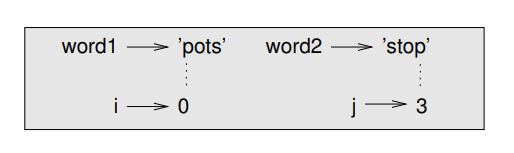
\includegraphics[width=0.5\textwidth]{./images/chapter_8_2.png}
        \caption{Turtle Pies.}
        \label{fig:8_2}
        \end{figure}

\section{Glosario}

\begin{description}
\item[objeto:] Algo a lo que una variable puede referirse. Por ahora, puedes usar "objeto" y "valor" indistintamente.
\item[secuencia:] Una colección ordenada de valores donde cada valor se identifica por un índice entero.
\item[elemento:] Uno de los valores en una secuencia.
\item[índice:] Un valor entero utilizado para seleccionar un elemento en una secuencia, como un carácter en una cadena. En Python, los índices comienzan desde 0.
\item[slice:] Una parte de una cadena especificada por un rango de índices.
\item[cadena vacía:] Una cadena sin caracteres y de longitud 0, representada por dos comillas.
\item[inmutable:] La propiedad de una secuencia cuyos elementos no pueden cambiarse.
\item[recorrer:] Iterar a través de los elementos en una secuencia, realizando una operación similar en cada uno.
\item[búsqueda:] Un patrón de recorrido que se detiene cuando encuentra lo que está buscando.
\item[contador:] Una variable utilizada para contar algo, generalmente inicializada a cero y luego incrementada.
\item[invocación:] Una sentencia que llama a un método.
\item[argumento opcional:] Un argumento de función o método que no es obligatorio.
\end{description}

\section{Ejercicios}

\textbf{Ejercicio 8.1.} Lee la documentación de los métodos de cadena en \url{http://docs.python.org/3/library/stdtypes.html#string-methods}. Es posible que desees experimentar con algunos de ellos para asegurarte de que entiendes cómo funcionan. \texttt{strip} y \texttt{replace} son particularmente útiles.

La documentación utiliza una sintaxis que podría ser confusa. Por ejemplo, en \texttt{find(sub[, start[, end]])}, los corchetes indican argumentos opcionales. Entonces \texttt{sub} es obligatorio, pero \texttt{start} es opcional, y si incluyes \texttt{start}, entonces \texttt{end} es opcional.

\textbf{Ejercicio 8.2.} Hay un método de cadena llamado \texttt{count} que es similar a la función en la Sección 8.7. Lee la documentación de este método y escribe una invocación que cuente el número de a's en 'banana'.

\textbf{Ejercicio 8.3.} Un slice de cadena puede tomar un tercer índice que especifica el "tamaño del paso"; es decir, el número de espacios entre caracteres sucesivos. Un tamaño de paso de 2 significa cada segundo carácter; 3 significa cada tercero, etc.

\begin{lstlisting}[language=Python]
>>> fruit = 'banana'
>>> fruit[0:5:2]
'bmn'
\end{lstlisting}

Un tamaño de paso de -1 recorre la palabra hacia atrás, por lo que el slice \texttt{[::-1]} genera una cadena invertida.

Usa este modismo para escribir una versión en una sola línea de \texttt{is\_palindrome} del Ejercicio 6.3.

\textbf{Ejercicio 8.4.} Las siguientes funciones están destinadas a verificar si una cadena contiene letras minúsculas, pero al menos algunas de ellas son incorrectas. Para cada función, describe qué hace realmente la función (asumiendo que el parámetro es una cadena).

\begin{lstlisting}[language=Python]
def any_lowercase1(s):
    for c in s:
        if c.islower():
            return True
        else:
            return False

def any_lowercase2(s):
    for c in s:
        if 'c'.islower():
            return 'True'
        else:
            return 'False'

def any_lowercase3(s):
    for c in s:
        flag = c.islower()
    return flag

def any_lowercase4(s):
    flag = False
    for c in s:
        flag = flag or c.islower()
    return flag

def any_lowercase5(s):
    for c in s:
        if not c.islower():
            return False
    return True
\end{lstlisting}

\textbf{Ejercicio 8.5.} Un cifrado César es una forma débil de encriptación que implica ``rotar'' cada letra por un número fijo de lugares. Rotar una letra significa desplazarla a través del alfabeto, volviendo al principio si es necesario, de modo que \texttt{'A'} rotada por 3 es \texttt{'D'} y \texttt{'Z'} rotada por 1 es \texttt{'A'}.

Para rotar una palabra, rota cada letra por la misma cantidad. Por ejemplo, \texttt{"cheer"} rotada por 7 es \texttt{"jolly"} y \texttt{"melon"} rotada por -10 es \texttt{"cubed"}. En la película \textit{2001: Una odisea del espacio}, la computadora de la nave se llama \texttt{HAL}, que es \texttt{IBM} rotada por -1.

Escribe una función llamada \texttt{rotate\_word} que tome una cadena y un entero como parámetros, y devuelva una nueva cadena que contenga las letras de la cadena original rotadas por la cantidad dada.

Es posible que desees usar la función incorporada \texttt{ord}, que convierte un carácter en un código numérico, y \texttt{chr}, que convierte códigos numéricos en caracteres. Las letras del alfabeto están codificadas en orden alfabético, por lo que, por ejemplo:

\begin{lstlisting}[language=Python]
>>> ord('c') - ord('a')
2
\end{lstlisting}

Porque 'c' es la segunda letra del alfabeto. Pero ten cuidado: los códigos numéricos para las letras mayúsculas son diferentes.

Los chistes potencialmente ofensivos en Internet a veces están codificados en ROT13, que es un cifrado César con rotación 13. Si no te ofendes fácilmente, busca y decodifica algunos de ellos. Solución: \url{https://thinkpython.com/code/rotate.py}.
\chapter{Caso de estudio: juegos de palabras}

Este capítulo presenta el segundo caso de estudio, que implica resolver acertijos de palabras buscando palabras que tengan ciertas propiedades. Por ejemplo, encontraremos los palíndromos más largos en inglés y buscaremos palabras cuyas letras aparezcan en orden alfabético. Además, presentaré otro plan de desarrollo de programas: reducción a un problema previamente resuelto.

\section{Lectura de listas de palabras}

Para los ejercicios de este capítulo necesitamos una lista de palabras en inglés. Hay muchas listas de palabras disponibles en la web, pero la más adecuada para nuestro propósito es una de las listas recopiladas y contribuidas al dominio público por Grady Ward como parte del proyecto Moby lexicon (ver \url{http://wikipedia.org/wiki/Moby_Project}). Es una lista de 113,809 palabras oficiales para crucigramas; es decir, palabras que se consideran válidas en crucigramas y otros juegos de palabras. En la colección Moby, el nombre del archivo es 113809of.fic; puedes descargar una copia, con el nombre más simple words.txt, desde \url{https://thinkpython.com/code/words.txt}.

Este archivo está en texto plano, por lo que puedes abrirlo con un editor de texto, pero también puedes leerlo desde Python. La función incorporada \texttt{open} toma el nombre del archivo como parámetro y devuelve un \textbf{objeto de archivo} que puedes usar para leer el archivo.

\begin{lstlisting}[language=Python]
>>> fin = open('words.txt')
\end{lstlisting}

\texttt{fin} es un nombre común para un objeto de archivo usado para entrada. El objeto de archivo proporciona varios métodos para lectura, incluido \texttt{readline}, que lee caracteres del archivo hasta llegar a un salto de línea y devuelve el resultado como una cadena:

\begin{lstlisting}[language=Python]
>>> fin.readline()
'aa\n'
\end{lstlisting}

La primera palabra en esta lista particular es "aa", que es un tipo de lava. La secuencia \texttt{\textbackslash n} representa el carácter de nueva línea que separa esta palabra de la siguiente.

El objeto de archivo realiza un seguimiento de su posición en el archivo, por lo que si llamas a \texttt{readline} nuevamente, obtienes la siguiente palabra:

\begin{lstlisting}[language=Python]
>>> fin.readline()
'aah\n'
\end{lstlisting}

La siguiente palabra es "aah", que es una palabra perfectamente legítima. O, si es el carácter de nueva línea lo que te molesta, podemos eliminarlo con el método de cadena \texttt{strip}:

\begin{lstlisting}[language=Python]
>>> line = fin.readline()
>>> word = line.strip()
>>> word
'aahed'
\end{lstlisting}

También puedes usar un objeto de archivo como parte de un bucle \texttt{for}. Este programa lee words.txt e imprime cada palabra, una por línea:

\begin{lstlisting}[language=Python]
fin = open('words.txt')
for line in fin:
    word = line.strip()
    print(word)
\end{lstlisting}

\section{Ejercicios}

Hay soluciones a estos ejercicios en la siguiente sección. Debes intentar cada uno al menos una vez antes de leer las soluciones.

\textbf{Ejercicio 9.1.} \textit{Escribe un programa que lea words.txt e imprima solo las palabras con más de 20 caracteres (sin contar espacios en blanco).}

\textbf{Ejercicio 9.2.} 

\textit{En 1939, Ernest Vincent Wright publicó una novela de 50,000 palabras titulada \textit{Gadsby}, que no contiene la letra "e". Dado que "e" es la letra más común en inglés, lograrlo no fue fácil.}

\textit{De hecho, es complicado construir una frase completa sin utilizar ese símbolo tan frecuente. Al principio puede ser lento, pero con práctica y cuidado se puede lograr fluidez gradualmente.}

\textit{Bueno, mejor me detengo.}

\textit{Escribe una función llamada \texttt{has\_no\_e} que devuelva \texttt{True} si la palabra dada no contiene la letra "e".}

\textit{Escribe un programa que lea el archivo \texttt{words.txt} e imprima solo las palabras que no contienen "e". Calcula también el porcentaje de palabras en la lista que no contienen dicha letra.}

\textbf{Ejercicio 9.3.} \textit{Escribe una función llamada \texttt{avoids} que tome una palabra y una cadena de letras prohibidas, y que devuelva \texttt{True} si la palabra no usa ninguna de las letras prohibidas.}

\textit{Escribe un programa que solicite al usuario ingresar una cadena de letras prohibidas y luego imprima el número de palabras que no contienen ninguna de ellas. ¿Puedes encontrar una combinación de 5 letras prohibidas que excluya la menor cantidad de palabras?}

\textbf{Ejercicio 9.4.} \textit{Escribe una función llamada \texttt{uses\_only} que tome una palabra y una cadena de letras, y que devuelva \texttt{True} si la palabra contiene solo letras en la lista. ¿Puedes hacer una oración usando solo las letras acefhlo? ¿Otra que no sea "Hoe alfalfa"?}

\textbf{Ejercicio 9.5.} \textit{Escribe una función llamada \texttt{uses\_all} que tome una palabra y una cadena de letras requeridas, y que devuelva \texttt{True} si la palabra usa todas las letras requeridas al menos una vez. ¿Cuántas palabras hay que usen todas las vocales aeiou? ¿Y aeiouy?}

\textbf{Ejercicio 9.6.} \textit{Escribe una función llamada \texttt{is\_abecedarian} que devuelva \texttt{True} si las letras de una palabra aparecen en orden alfabético (se permiten letras dobles). ¿Cuántas palabras abecedarian hay?}

\section{Búsqueda}

Todos los ejercicios de la sección anterior tienen algo en común; pueden resolverse con el patrón de búsqueda que vimos en la Sección 8.6. El ejemplo más simple es:

\begin{lstlisting}[language=Python]
def has_no_e(word):
    for letter in word:
        if letter == 'e':
            return False
    return True
\end{lstlisting}

El bucle \texttt{for} recorre los caracteres en \texttt{word}. Si encontramos la letra "e", podemos devolver \texttt{False} inmediatamente; de lo contrario, tenemos que pasar a la siguiente letra. Si salimos del bucle normalmente, significa que no encontramos una "e", por lo que devolvemos \texttt{True}.

Podrías escribir esta función de manera más concisa usando el operador \texttt{in}, pero comencé con esta versión porque demuestra la lógica del patrón de búsqueda.

\texttt{avoids} es una versión más general de \texttt{has\_no\_e} pero tiene la misma estructura:

\begin{lstlisting}[language=Python]
def avoids(word, forbidden):
    for letter in word:
        if letter in forbidden:
            return False
    return True
\end{lstlisting}

Podemos devolver \texttt{False} tan pronto como encontremos una letra prohibida; si llegamos al final del bucle, devolvemos \texttt{True}.

\texttt{uses\_only} es similar excepto que el sentido de la condición está invertido:

\begin{lstlisting}[language=Python]
def uses_only(word, available):
    for letter in word:
        if letter not in available:
            return False
    return True
\end{lstlisting}

En lugar de una lista de letras prohibidas, tenemos una lista de letras disponibles. Si encontramos una letra en \texttt{word} que no está en \texttt{available}, podemos devolver \texttt{False}.

\texttt{uses\_all} es similar excepto que invertimos el rol de la palabra y la cadena de letras:

\begin{lstlisting}[language=Python]
def uses_all(word, required):
    for letter in required:
        if letter not in word:
            return False
    return True
\end{lstlisting}

En lugar de recorrer las letras en \texttt{word}, el bucle recorre las letras requeridas. Si alguna de las letras requeridas no aparece en la palabra, podemos devolver \texttt{False}.

Si realmente estuvieras pensando como un informático, habrías reconocido que \texttt{uses\_all} era una instancia de un problema previamente resuelto, y habrías escrito:

\begin{lstlisting}[language=Python]
def uses_all(word, required):
    return uses_only(required, word)
\end{lstlisting}

Este es un ejemplo de un plan de desarrollo de programas llamado reducción a un problema previamente resuelto, lo que significa que reconoces el problema en el que estás trabajando como una instancia de un problema resuelto y aplicas una solución existente.

\section{Bucles con índices}

Escribí las funciones en la sección anterior con bucles \texttt{for} porque solo necesitaba los caracteres en las cadenas; no tenía que hacer nada con los índices.

Para \texttt{is\_abecedarian} tenemos que comparar letras adyacentes, lo cual es un poco complicado con un bucle \texttt{for}:

\begin{lstlisting}[language=Python]
def is_abecedarian(word):
    previous = word[0]
    for c in word:
        if c < previous:
            return False
        previous = c
    return True
\end{lstlisting}

Una alternativa es usar recursión:

\begin{lstlisting}[language=Python]
def is_abecedarian(word):
    if len(word) <= 1:
        return True
    if word[0] > word[1]:
        return False
    return is_abecedarian(word[1:])
\end{lstlisting}

Otra opción es usar un bucle \texttt{while}:

\begin{lstlisting}[language=Python]
def is_abecedarian(word):
    i = 0
    while i < len(word)-1:
        if word[i+1] < word[i]:
            return False
        i = i+1
    return True
\end{lstlisting}

El bucle comienza en \texttt{i=0} y termina cuando \texttt{i=len(word)-1}. Cada vez que se ejecuta el bucle, compara el carácter \texttt{i-ésimo} (que puedes pensar como el carácter actual) con el carácter \texttt{i+1-ésimo} (que puedes pensar como el siguiente).

Si el siguiente carácter es menor (alfabéticamente anterior) que el actual, entonces hemos descubierto un rompimiento en la tendencia abecedariana, y devolvemos \texttt{False}.

Si llegamos al final del bucle sin encontrar fallas, entonces la palabra pasa la prueba. Para convencerte de que el bucle termina correctamente, considera un ejemplo como 'flossy'. La longitud de la palabra es 6, por lo que la última vez que se ejecuta el bucle es cuando \texttt{i} es 4, que es el índice del penúltimo carácter. En la última iteración, compara el penúltimo carácter con el último, que es lo que queremos.

Aquí hay una versión de \texttt{is\_palindrome} (ver Ejercicio 6.3) que usa dos índices; uno comienza al principio y avanza; el otro comienza al final y retrocede.

\begin{lstlisting}[language=Python]
def is_palindrome(word):
    i = 0
    j = len(word)-1
    while i<j:
        if word[i] != word[j]:
            return False
        i = i+1
        j = j-1
    return True
\end{lstlisting}

O podríamos reducir a un problema previamente resuelto y escribir:

\begin{lstlisting}[language=Python]
def is_palindrome(word):
    return is_reverse(word, word)
\end{lstlisting}

Usando \texttt{is\_reverse} de la Sección 8.11.

\section{Depuración}

Probar programas es difícil. Las funciones de este capítulo son relativamente fáciles de probar porque puedes verificar los resultados manualmente. Aun así, está entre difícil e imposible elegir un conjunto de palabras que prueben todos los errores posibles.

Tomando \texttt{has\_no\_e} como ejemplo, hay dos casos obvios para verificar: palabras que tienen una 'e' deberían devolver \texttt{False}, y palabras que no la tienen deberían devolver \texttt{True}. No deberías tener problemas para encontrar una de cada.

Dentro de cada caso, hay algunos subcasos menos obvios. Entre las palabras que tienen una "e", deberías probar palabras con una "e" al principio, al final y en algún lugar intermedio. Deberías probar palabras largas, palabras cortas y palabras muy cortas, como la cadena vacía. La cadena vacía es un ejemplo de un caso especial, que es uno de los casos no obvios donde a menudo se esconden errores.

Además de los casos de prueba que generes, también puedes probar tu programa con una lista de palabras como words.txt. Al escanear la salida, podrías detectar errores, pero ten cuidado: podrías detectar un tipo de error (palabras que no deberían incluirse, pero lo están) y no otro (palabras que deberían incluirse, pero no lo están).

En general, las pruebas pueden ayudarte a encontrar errores, pero no es fácil generar un buen conjunto de casos de prueba, e incluso si lo haces, no puedes estar seguro de que tu programa sea correcto. Según un legendario informático:

\begin{quote}
¡Las pruebas de programas pueden usarse para mostrar la presencia de errores, pero nunca para mostrar su ausencia!
— Edsger W. Dijkstra
\end{quote}

\section{Glosario}

\textbf{objeto de archivo:} Un valor que representa un archivo abierto.

\textbf{reducción a un problema previamente resuelto:} Una forma de resolver un problema expresándolo como una instancia de un problema previamente resuelto.

\textbf{caso especial:} Un caso de prueba que es atípico o no obvio (y menos probable que se maneje correctamente).

\section{Ejercicios}

\textbf{Ejercicio 9.7.} Esta pregunta está basada en un Puzzler que fue transmitido en el programa de radio Car Talk (\url{http://www.cartalk.com/content/puzzlers}):

\textit{Dame una palabra con tres pares de letras consecutivos. Te daré un par de palabras que casi califican, pero no. Por ejemplo, la palabra committee, c-o-m-m-i-t-t-e-e. Sería genial excepto por la 'i' que se cuela allí. O Mississippi: M-i-s-s-i-s-s-i-p-p-i. Si pudieras quitar esas i's funcionaría. Pero hay una palabra que tiene tres pares consecutivos de letras y que, hasta donde sé, puede ser la única. Por supuesto, probablemente hay 500 más, pero solo puedo pensar en una. ¿Cuál es la palabra?}

Escribe un programa para encontrarla. Solución: \url{https://thinkpython.com/code/cartalk1.py}.

\textbf{Ejercicio 9.8.} Aquí hay otro Puzzler de Car Talk (\url{http://www.cartalk.com/content/puzzlers}):

\textit{"Estaba conduciendo por la autopista el otro día y noté mi odómetro. Como la mayoría de los odómetros, muestra seis dígitos, en millas enteras solamente. Así que, si mi auto tuviera 300,000 millas, por ejemplo, vería 3-0-0-0-0-0."}

\textit{"Lo que vi ese día fue muy interesante. Noté que los últimos 4 dígitos eran palíndromos; es decir, se leían igual hacia adelante que hacia atrás. Por ejemplo, 5-4-4-5 es un palíndromo, por lo que mi odómetro podría haber leído 3-1-5-4-4-5."}

\textit{"Una milla después, los últimos 5 números eran palíndromos. Por ejemplo, podría haber leído 3-6-5-4-5-6. Una milla después de eso, los 4 números centrales de los 6 eran palíndromos. ¿Y están listos para esto? Una milla después, ¡los 6 eran palíndromos!"}

\textit{"La pregunta es, ¿qué marcaba el odómetro cuando lo miré por primera vez?"}

Escribe un programa en Python que pruebe todos los números de seis dígitos e imprima los números que satisfacen estos requisitos. Solución: \url{https://thinkpython.com/code/cartalk2.py}.

\textbf{Ejercicio 9.9.} Aquí hay otro Puzzler de Car Talk que puedes resolver con una búsqueda (\url{http://www.cartalk.com/content/puzzlers}):

\textit{"Recientemente visité a mi mamá y nos dimos cuenta de que los dos dígitos que conforman mi edad cuando se invierten resultan en su edad. Por ejemplo, si ella tiene 73, yo tengo 37. Nos preguntamos cuántas veces ha sucedido esto a lo largo de los años, pero nos distrajimos con otros temas y nunca llegamos a una respuesta."}

\textit{"Cuando llegué a casa, descubrí que los dígitos de nuestras edades han sido reversibles seis veces hasta ahora. También descubrí que, si tenemos suerte, sucederá nuevamente en unos años, y si tenemos mucha suerte, sucederá una vez más después de eso. En otras palabras, habrá sucedido 8 veces en total. Entonces la pregunta es, ¿cuántos años tengo ahora?"}

Escribe un programa en Python que busque soluciones a este Puzzler. Pista: podrías encontrar útil el método de cadena \texttt{zfill}.

Solución: \url{https://thinkpython.com/code/cartalk3.py}.
%Chapter 10
\chapter{Listas}

Este capítulo presenta uno de los tipos integrados más útiles de Python: las listas. También aprenderás más sobre objetos y lo que puede suceder cuando tienes más de un nombre para el mismo objeto.

\section{Una lista es una secuencia}

Al igual que una cadena, una lista es una secuencia de valores. En una cadena, los valores son caracteres; en una lista, pueden ser de cualquier tipo. Los valores en una lista se llaman \textbf{elementos} o, a veces, \textbf{ítems}.

Hay varias formas de crear una nueva lista; la más simple es encerrar los elementos entre corchetes ([ y ]):

\begin{lstlisting}[language=Python]
[10, 20, 30, 40]  
['crunchy frog', 'ram bladder', 'lark vomit']  
\end{lstlisting}

El primer ejemplo es una lista de cuatro enteros. El segundo es una lista de tres cadenas. Los elementos de una lista no tienen que ser del mismo tipo. La siguiente lista contiene una cadena, un flotante, un entero y (¡oh!) otra lista:

\begin{lstlisting}[language=Python]
['spam', 2.0, 5, [10, 20]]
\end{lstlisting}

Una lista dentro de otra lista se llama \textbf{lista anidada}.

Una lista que no contiene elementos se llama \textbf{lista vacía}; puedes crear una con corchetes vacíos, [].

Como era de esperar, puedes asignar valores de lista a variables:

\begin{lstlisting}[language=Python]
>>> cheeses = ['Cheddar', 'Edam', 'Gouda']  
>>> numbers = [42, 123]  
>>> empty = []  

>>> print(cheeses, numbers, empty)  
['Cheddar', 'Edam', 'Gouda'] [42, 123]
\end{lstlisting}
\begin{figure}[h]
        \centering
        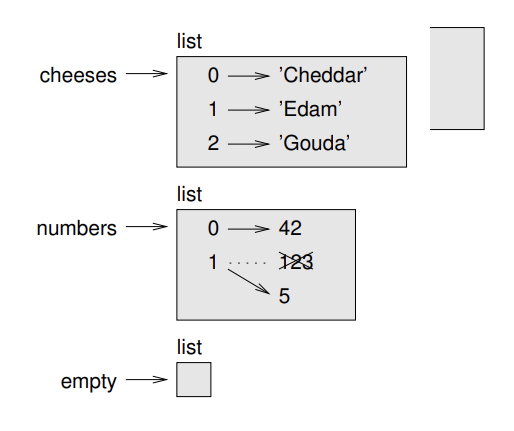
\includegraphics[width=0.5\textwidth]{./images/chapter_10_1.png}
        \caption{Diagrama de estados.}
        \label{fig:10_1}
        \end{figure}
\section{Las listas son mutables}

La sintaxis para acceder a los elementos de una lista es la misma que para acceder a los caracteres de una cadena: el operador de corchetes. La expresión dentro de los corchetes especifica el índice. Recuerda que los índices comienzan en 0:

\begin{lstlisting}[language=Python]
>>> cheeses[0] 
'Cheddar'
\end{lstlisting}

A diferencia de las cadenas, las listas son mutables. Cuando el operador de corchetes aparece en el lado izquierdo de una asignación, identifica el elemento de la lista que será asignado.

\begin{lstlisting}[language=Python]
>>> numbers = [42, 123] 
>>> numbers[1] = 5 
>>> numbers 
[42, 5]
\end{lstlisting}

El elemento en la posición 1 de \texttt{numbers}, que solía ser 123, ahora es 5.

Los índices de lista funcionan de la misma manera que los índices de cadena:

\begin{itemize}
    \item Cualquier expresión entera puede usarse como índice.
    \item Si intentas leer o escribir un elemento que no existe, obtienes un \texttt{IndexError}.
    \item Si un índice tiene un valor negativo, cuenta hacia atrás desde el final de la lista.
\end{itemize}

El operador \texttt{in} también funciona con listas.

\begin{lstlisting}[language=Python]
>>> cheeses = ['Cheddar', 'Edam', 'Gouda'] 
>>> 'Edam' in cheeses 
True 
>>> 'Brie' in cheeses 
False
\end{lstlisting}

\section{Recorriendo una lista}

La forma más común de recorrer los elementos de una lista es con un bucle \texttt{for}. La sintaxis es la misma que para cadenas:

\begin{lstlisting}[language=Python]
for cheese in cheeses:
    print(cheese)
\end{lstlisting}

Esto funciona bien si solo necesitas leer los elementos de la lista. Pero si quieres escribir o actualizar los elementos, necesitas los índices. Una forma común de hacerlo es combinar las funciones integradas \texttt{range} y \texttt{len}:

\begin{lstlisting}[language=Python]
for i in range(len(numbers)):
    numbers[i] = numbers[i] * 2
\end{lstlisting}

Este bucle recorre la lista y actualiza cada elemento. \texttt{len} devuelve el número de elementos en la lista. \texttt{range} devuelve una lista de índices desde 0 hasta \(n-1\), donde \(n\) es la longitud de la lista. Cada vez que se ejecuta el bucle, \texttt{i} obtiene el índice del siguiente elemento. La declaración de asignación en el cuerpo usa \texttt{i} para leer el valor antiguo del elemento y asignar el nuevo valor.

Un bucle \texttt{for} sobre una lista vacía nunca ejecuta el cuerpo:

\begin{lstlisting}[language=Python]
for x in []:
    print('This never happens.')
\end{lstlisting}

Aunque una lista puede contener otra lista, la lista anidada todavía cuenta como un solo elemento. La longitud de esta lista es cuatro:

\begin{lstlisting}[language=Python]
['spam', 1, ['Brie', 'Roquefort', 'Pol le Veq'], [1, 2, 3]]
\end{lstlisting}

\section{Operaciones con listas}

El operador \texttt{+} concatena listas:

\begin{lstlisting}[language=Python]
>>> a = [1, 2, 3] 
>>> b = [4, 5, 6] 
>>> c = a + b 
>>> c 
[1, 2, 3, 4, 5, 6]
\end{lstlisting}

El operador \texttt{*} repite una lista un número determinado de veces:

\begin{lstlisting}[language=Python]
>>> [0] * 4 
[0, 0, 0, 0] 
>>> [1, 2, 3] * 3 
[1, 2, 3, 1, 2, 3, 1, 2, 3]
\end{lstlisting}

El primer ejemplo repite \texttt{[0]} cuatro veces. El segundo ejemplo repite la lista \texttt{[1, 2, 3]} tres veces.

\section{Segmentos de lista}

El operador de segmento también funciona con listas:

\begin{lstlisting}[language=Python]
>>> t = ['a', 'b', 'c', 'd', 'e', 'f'] 
>>> t[1:3] 
['b', 'c'] 
>>> t[:4] 
['a', 'b', 'c', 'd'] 
>>> t[3:] 
['d', 'e', 'f']
\end{lstlisting}

Si omites el primer índice, el segmento comienza al principio. Si omites el segundo, el segmento va hasta el final. Si omites ambos, el segmento es una copia de toda la lista.

\begin{lstlisting}[language=Python]
>>> t[:] 
['a', 'b', 'c', 'd', 'e', 'f']
\end{lstlisting}

Dado que las listas son mutables, a menudo es útil hacer una copia antes de realizar operaciones que modifiquen listas.

Un operador de segmento en el lado izquierdo de una asignación puede actualizar múltiples elementos:

\begin{lstlisting}[language=Python]
>>> t = ['a', 'b', 'c', 'd', 'e', 'f'] 
>>> t[1:3] = ['x', 'y'] 
>>> t 
['a', 'x', 'y', 'd', 'e', 'f']
\end{lstlisting}

\section{Métodos de lista}

Python proporciona métodos que operan en listas. Por ejemplo, \texttt{append} agrega un nuevo elemento al final de una lista:

\begin{lstlisting}[language=Python]
>>> t = ['a', 'b', 'c'] 
>>> t.append('d') 
>>> t 
['a', 'b', 'c', 'd']
\end{lstlisting}

\texttt{extend} toma una lista como argumento y agrega todos sus elementos:

\begin{lstlisting}[language=Python]
>>> t1 = ['a', 'b', 'c'] 
>>> t2 = ['d', 'e'] 
>>> t1.extend(t2) 
>>> t1 
['a', 'b', 'c', 'd', 'e']
\end{lstlisting}

Este ejemplo deja \texttt{t2} sin modificar.

\texttt{sort} ordena los elementos de la lista de menor a mayor:

\begin{lstlisting}[language=Python]
>>> t = ['d', 'c', 'e', 'b', 'a'] 
>>> t.sort() 
>>> t 
['a', 'b', 'c', 'd', 'e']
\end{lstlisting}

La mayoría de los métodos de lista son nulos; modifican la lista y devuelven \texttt{None}. Si accidentalmente escribes \texttt{t = t.sort()}, te decepcionará el resultado.

\section{Map, filter y reduce}

Para sumar todos los números en una lista, puedes usar un bucle como este:

\begin{lstlisting}[language=Python]
def add_all(t):
    total = 0
    for x in t:
        total += x
    return total
\end{lstlisting}

\texttt{total} se inicializa en 0. Cada vez que se ejecuta el bucle, \texttt{x} obtiene un elemento de la lista. El operador \texttt{+=} proporciona una forma abreviada de actualizar una variable. Esta declaración de asignación aumentada,

\begin{lstlisting}[language=Python]
total += x
\end{lstlisting}

es equivalente a

\begin{lstlisting}[language=Python]
total = total + x
\end{lstlisting}

A medida que se ejecuta el bucle, \texttt{total} acumula la suma de los elementos; una variable usada de esta manera a veces se llama \textbf{acumulador}.

Sumar los elementos de una lista es una operación tan común que Python la proporciona como una función integrada, \texttt{sum}:

\begin{lstlisting}[language=Python]
>>> t = [1, 2, 3] 
>>> sum(t) 
6
\end{lstlisting}

Una operación como esta que combina una secuencia de elementos en un solo valor a veces se llama \textbf{reduce}.

A veces quieres recorrer una lista mientras construyes otra. Por ejemplo, la siguiente función toma una lista de cadenas y devuelve una nueva lista que contiene las cadenas en mayúsculas:

\begin{lstlisting}[language=Python]
def capitalize_all(t):
    res = []
    for s in t:
        res.append(s.capitalize())
    return res
\end{lstlisting}

\texttt{res} se inicializa con una lista vacía; cada vez que se ejecuta el bucle, agregamos el siguiente elemento. Así que \texttt{res} es otro tipo de acumulador.

Una operación como \texttt{capitalize\_all} a veces se llama \textbf{map} porque "mapea" una función (en este caso, el método \texttt{capitalize}) sobre cada uno de los elementos en una secuencia.

Otra operación común es seleccionar algunos elementos de una lista y devolver una sublista. Por ejemplo, la siguiente función toma una lista de cadenas y devuelve una lista que contiene solo las cadenas en mayúsculas:

\begin{lstlisting}[language=Python]
def only_upper(t):
    res = []
    for s in t:
        if s.isupper():
            res.append(s)
    return res
\end{lstlisting}

\texttt{isupper} es un método de cadena que devuelve \texttt{True} si la cadena contiene solo letras mayúsculas. Una operación como \texttt{only\_upper} se llama \textbf{filter} porque selecciona algunos de los elementos y filtra los demás. La mayoría de las operaciones comunes de listas se pueden expresar como una combinación de \texttt{map}, \texttt{filter} y \texttt{reduce}.

\section{Eliminando elementos}

Hay varias formas de eliminar elementos de una lista. Si conoces el índice del elemento que deseas eliminar, puedes usar \texttt{pop}:

\begin{lstlisting}[language=Python]
>>> t = ['a', 'b', 'c'] 
>>> x = t.pop(1) 
>>> t 
['a', 'c'] 
>>> x 
'b'
\end{lstlisting}

\texttt{pop} modifica la lista y devuelve el elemento que fue eliminado. Si no proporcionas un índice, elimina y devuelve el último elemento.

Si no necesitas el valor eliminado, puedes usar el operador \texttt{del}:

\begin{lstlisting}[language=Python]
>>> t = ['a', 'b', 'c'] 
>>> del t[1] 
>>> t 
['a', 'c']
\end{lstlisting}

Si conoces el elemento que deseas eliminar (pero no el índice), puedes usar \texttt{remove}:

\begin{lstlisting}[language=Python]
>>> t = ['a', 'b', 'c'] 
>>> t.remove('b') 
>>> t 
['a', 'c']
\end{lstlisting}

El valor de retorno de \texttt{remove} es \texttt{None}.

Para eliminar más de un elemento, puedes usar \texttt{del} con un índice de segmento:

\begin{lstlisting}[language=Python]
>>> t = ['a', 'b', 'c', 'd', 'e', 'f'] 
>>> del t[1:5] 
>>> t 
['a', 'f']
\end{lstlisting}

Como es habitual, el segmento selecciona todos los elementos hasta, pero sin incluir, el segundo índice.

\section{Listas y cadenas}

Una cadena es una secuencia de caracteres y una lista es una secuencia de valores, pero una lista de caracteres no es lo mismo que una cadena. Para convertir una cadena en una lista de caracteres, puedes usar \texttt{list}:

\begin{lstlisting}[language=Python]
>>> s = 'spam' 
>>> t = list(s) 
>>> t 
['s', 'p', 'a', 'm']
\end{lstlisting}

\begin{figure}[h]
        \centering
        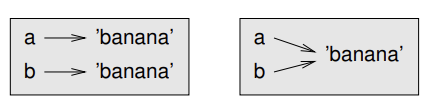
\includegraphics[width=0.5\textwidth]{./images/chapter_10_2.png}
        \caption{Diagrama de estados.}
        \label{fig:10_2}
        \end{figure}


Dado que \texttt{list} es el nombre de una función integrada, debes evitar usarlo como nombre de variable. También evito \texttt{l} porque se parece demasiado a \texttt{1}. Por eso uso \texttt{t}.

La función \texttt{list} divide una cadena en letras individuales. Si deseas dividir una cadena en palabras, puedes usar el método \texttt{split}:

\begin{lstlisting}[language=Python]
>>> s = 'pining for the fjords' 
>>> t = s.split() 
>>> t 
['pining', 'for', 'the', 'fjords']
\end{lstlisting}

Un argumento opcional llamado \textbf{delimitador} especifica qué caracteres usar como límites de palabras. El siguiente ejemplo usa un guión como delimitador:

\begin{lstlisting}[language=Python]
>>> s = 'spam-spam-spam' 
>>> delimiter = '-' 
>>> t = s.split(delimiter) 
>>> t 
['spam', 'spam', 'spam']
\end{lstlisting}

\texttt{join} es el inverso de \texttt{split}. Toma una lista de cadenas y concatena los elementos. \texttt{join} es un método de cadena, por lo que debes invocarlo en el delimitador y pasar la lista como parámetro:

\begin{lstlisting}[language=Python]
>>> t = ['pining', 'for', 'the', 'fjords'] 
>>> delimiter = ' ' 
>>> s = delimiter.join(t) 
>>> s 
'pining for the fjords'
\end{lstlisting}

En este caso, el delimitador es un espacio, por lo que \texttt{join} coloca un espacio entre las palabras. Para concatenar cadenas sin espacios, puedes usar la cadena vacía, \texttt{''}, como delimitador.

\section{Objetos y valores}

Si ejecutamos estas declaraciones de asignación:

\begin{lstlisting}[language=Python]
a = 'banana'
b = 'banana'
\end{lstlisting}

Sabemos que \texttt{a} y \texttt{b} se refieren a una cadena, pero no sabemos si se refieren a la misma cadena. Hay dos estados posibles:

En un caso, \texttt{a} y \texttt{b} se refieren a dos objetos diferentes que tienen el mismo valor. En el segundo caso, se refieren al mismo objeto.

Para verificar si dos variables se refieren al mismo objeto, puedes usar el operador \texttt{is}:
\begin{figure}[h]
        \centering
        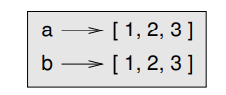
\includegraphics[width=0.5\textwidth]{./images/chapter_10_3.png}
        \caption{Diagrama de estados.}
        \label{fig:10_3}
        \end{figure}

\begin{figure}[h]
        \centering
        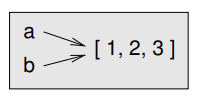
\includegraphics[width=0.5\textwidth]{./images/chapter_10_4.png}
        \caption{Diagrama de estados.}
        \label{fig:10_4}
        \end{figure}

\begin{lstlisting}[language=Python]
>>> a = 'banana' 
>>> b = 'banana' 
>>> a is b 
True
\end{lstlisting}

En este ejemplo, Python solo creó un objeto de cadena, y tanto \texttt{a} como \texttt{b} se refieren a él. Pero cuando creas dos listas, obtienes dos objetos:

\begin{lstlisting}[language=Python]
>>> a = [1, 2, 3] 
>>> b = [1, 2, 3] 
>>> a is b 
False
\end{lstlisting}

En este caso, diríamos que las dos listas son \textbf{equivalentes}, porque tienen los mismos elementos, pero no \textbf{idénticas}, porque no son el mismo objeto. Si dos objetos son idénticos, también son equivalentes, pero si son equivalentes, no son necesariamente idénticos.

Hasta ahora, hemos estado usando "objeto" y "valor" indistintamente, pero es más preciso decir que un objeto tiene un valor. Si evalúas \texttt{[1, 2, 3]}, obtienes un objeto de lista cuyo valor es una secuencia de enteros. Si otra lista tiene los mismos elementos, decimos que tiene el mismo valor, pero no es el mismo objeto.

\section{Alias}

Si \texttt{a} se refiere a un objeto y asignas \texttt{b = a}, entonces ambas variables se refieren al mismo objeto:

\begin{lstlisting}[language=Python]
>>> a = [1, 2, 3] 
>>> b = a 
>>> b is a 
True
\end{lstlisting}

La asociación de una variable con un objeto se llama \textbf{referencia}. En este ejemplo, hay dos referencias al mismo objeto.

Un objeto con más de una referencia tiene más de un nombre, por lo que decimos que el objeto tiene un \textbf{alias}.

Si el objeto con alias es mutable, los cambios realizados con un alias afectan al otro:

\begin{figure}[h]
        \centering
        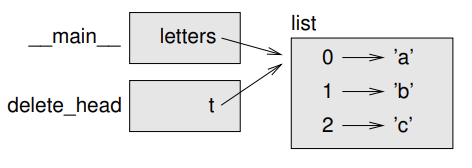
\includegraphics[width=0.5\textwidth]{./images/chapter_10_5.png}
        \caption{Diagrama de pila.}
        \label{fig:10_5}
        \end{figure}


\begin{lstlisting}[language=Python]
>>> b[0] = 42 
>>> a 
[42, 2, 3]
\end{lstlisting}

Aunque este comportamiento puede ser útil, es propenso a errores. En general, es más seguro evitar los alias cuando trabajas con objetos mutables.

Para objetos inmutables como cadenas, los alias no son un problema tan grande. En este ejemplo:

\begin{lstlisting}[language=Python]
a = 'banana'
b = 'banana'
\end{lstlisting}

Casi nunca importa si \texttt{a} y \texttt{b} se refieren a la misma cadena o no.

\section{Argumentos de lista}

Cuando pasas una lista a una función, la función obtiene una referencia a la lista. Si la función modifica la lista, el llamador ve el cambio. Por ejemplo, \texttt{delete\_head} elimina el primer elemento de una lista:

\begin{lstlisting}[language=Python]
def delete_head(t):
    del t[0]
\end{lstlisting}

Así es como se usa:

\begin{lstlisting}[language=Python]
>>> letters = ['a', 'b', 'c'] 
>>> delete_head(letters) 
>>> letters 
['b', 'c']
\end{lstlisting}

El parámetro \texttt{t} y la variable \texttt{letters} son alias para el mismo objeto.

Es importante distinguir entre operaciones que modifican listas y operaciones que crean nuevas listas. Por ejemplo, el método \texttt{append} modifica una lista, pero el operador \texttt{+} crea una nueva lista.

Aquí un ejemplo usando \texttt{append}:

\begin{lstlisting}[language=Python]
>>> t1 = [1, 2] 
>>> t2 = t1.append(3) 
>>> t1 
[1, 2, 3] 
>>> t2 
None
\end{lstlisting}

El valor de retorno de \texttt{append} es \texttt{None}.

Aquí un ejemplo usando el operador \texttt{+}:

\begin{lstlisting}[language=Python]
>>> t3 = t1 + [4] 
>>> t1 
[1, 2, 3] 
>>> t3 
[1, 2, 3, 4]
\end{lstlisting}

El resultado del operador es una nueva lista, y la lista original no cambia.

Esta diferencia es importante cuando escribes funciones que deben modificar listas. Por ejemplo, esta función \textbf{no} elimina la cabeza de una lista:

\begin{lstlisting}[language=Python]
def bad_delete_head(t):
    t = t[1:]  # !INCORRECTO
\end{lstlisting}


El operador de segmento crea una nueva lista y la asignación hace que \texttt{t} se refiera a ella, pero eso no afecta al llamador.

\begin{lstlisting}[language=Python]
>>> t4 = [1, 2, 3] 
>>> bad_delete_head(t4) 
>>> t4 
[1, 2, 3]
\end{lstlisting}

Al principio de \texttt{bad\_delete\_head}, \texttt{t} y \texttt{t4} se refieren a la misma lista. Al final, \texttt{t} se refiere a una nueva lista, pero \texttt{t4} todavía se refiere a la lista original sin modificar.

Una alternativa es escribir una función que cree y devuelva una nueva lista. Por ejemplo, \texttt{tail} devuelve todos los elementos excepto el primero de una lista:

\begin{lstlisting}[language=Python]
def tail(t):
    return t[1:]
\end{lstlisting}

Esta función deja la lista original sin modificar. Así es como se usa:

\begin{lstlisting}[language=Python]
>>> letters = ['a', 'b', 'c'] 
>>> rest = tail(letters) 
>>> rest 
['b', 'c']
\end{lstlisting}

\section{Depuración}

El uso descuidado de listas (y otros objetos mutables) puede llevar a largas horas de depuración. Aquí hay algunos errores comunes y formas de evitarlos:

\begin{enumerate}
    \item La mayoría de los métodos de lista modifican el argumento y devuelven \texttt{None}. Esto es lo opuesto a los métodos de cadena, que devuelven una nueva cadena y dejan el original intacto. Si estás acostumbrado a escribir código de cadena como este:
    
    \begin{lstlisting}[language=Python]
    word = word.strip()
    \end{lstlisting}
    
    Es tentador escribir código de lista como este:
    
    \begin{lstlisting}[language=Python]
    t = t.sort()  # !INCORRECTO
    \end{lstlisting}

    
    Debido a que \texttt{sort} devuelve \texttt{None}, la siguiente operación que realices con \texttt{t} probablemente fallará.
    
    Antes de usar métodos y operadores de lista, debes leer la documentación cuidadosamente y luego probarlos en modo interactivo.
    
    \item Elige un estilo y apégate a él.
    
    Parte del problema con las listas es que hay demasiadas formas de hacer las cosas. Por ejemplo, para eliminar un elemento de una lista, puedes usar \texttt{pop}, \texttt{remove}, \texttt{del} o incluso una asignación de segmento.
    
    Para agregar un elemento, puedes usar el método \texttt{append} o el operador \texttt{+}. Asumiendo que \texttt{t} es una lista y \texttt{x} es un elemento de lista, estos son correctos:
    
    \begin{lstlisting}[language=Python]
    t.append(x)
    t = t + [x]
    t += [x]
    \end{lstlisting}
    
    Y estos son incorrectos:
    
    \begin{lstlisting}[language=Python]
    t.append([x])     # ! INCORRECTO
    t = t.append(x)   # ! INCORRECTO
    t + [x]           # ! INCORRECTO
    t = t + x         # ! INCORRECTO
    \end{lstlisting}


    
    Prueba cada uno de estos ejemplos en modo interactivo para asegurarte de entender lo que hacen. Observa que solo el último causa un error en tiempo de ejecución; los otros tres son legales, pero hacen lo incorrecto.
    
    \item Haz copias para evitar alias.
    
    Si quieres usar un método como \texttt{sort} que modifica el argumento, pero necesitas mantener la lista original también, puedes hacer una copia.
    
    \begin{lstlisting}[language=Python]
    >>> t = [3, 1, 2] 
    >>> t2 = t[:] 
    >>> t2.sort() 
    >>> t 
    [3, 1, 2] 
    >>> t2 
    [1, 2, 3]
    \end{lstlisting}
    
    En este ejemplo, también podrías usar la función integrada \texttt{sorted}, que devuelve una nueva lista ordenada y deja la original intacta.
    
    \begin{lstlisting}[language=Python]
    >>> t2 = sorted(t) 
    >>> t 
    [3, 1, 2] 
    >>> t2 
    [1, 2, 3]
    \end{lstlisting}
\end{enumerate}

\section*{Glosario}

\begin{description}
    \item[lista:] Una secuencia de valores.
    \item[elemento:] Uno de los valores en una lista (u otra secuencia), también llamado ítem.
    \item[lista anidada:] Una lista que es un elemento de otra lista.
    \item[acumulador:] Una variable usada en un bucle para acumular un resultado.
    \item[asignación aumentada:] Una declaración que actualiza el valor de una variable usando un operador como \texttt{+=}.
    \item[reduce:] Un patrón de procesamiento que recorre una secuencia y acumula los elementos en un solo resultado.
    \item[map:] Un patrón de procesamiento que recorre una secuencia y realiza una operación en cada elemento.
    \item[filter:] Un patrón de procesamiento que recorre una lista y selecciona los elementos que satisfacen algún criterio.
    \item[objeto:] Algo a lo que una variable puede referirse. Un objeto tiene un tipo y un valor.
    \item[equivalente:] Que tiene el mismo valor.
    \item[idéntico:] Ser el mismo objeto (lo que implica equivalencia).
    \item[referencia:] La asociación entre una variable y su valor.
    \item[alias:] Una circunstancia donde dos o más variables se refieren al mismo objeto.
    \item[delimitador:] Un carácter o cadena usado para indicar dónde se debe dividir una cadena.
\end{description}

\section*{Ejercicios}

Puedes descargar soluciones a estos ejercicios desde \url{https://thinkpython.com/code/list_exercises.py}.

\begin{enumerate}
    \item \textbf{Ejercicio 10.1.} Escribe una función llamada \texttt{nested\_sum} que tome una lista de listas de enteros y sume los elementos de todas las listas anidadas. Por ejemplo:
    
    \begin{lstlisting}[language=Python]
    >>> t = [[1, 2], [3], [4, 5, 6]] 
    >>> nested_sum(t) 
    21
    \end{lstlisting}
    
    \item \textbf{Ejercicio 10.2.} Escribe una función llamada \texttt{cumsum} que tome una lista de números y devuelva la suma acumulativa; es decir, una nueva lista donde el elemento \(i\)-ésimo es la suma de los primeros \(i+1\) elementos de la lista original. Por ejemplo:
    
    \begin{lstlisting}[language=Python]
    >>> t = [1, 2, 3] 
    >>> cumsum(t) 
    [1, 3, 6]
    \end{lstlisting}
    
    \item \textbf{Ejercicio 10.3.} Escribe una función llamada \texttt{middle} que tome una lista y devuelva una nueva lista que contenga todos los elementos excepto el primero y el último. Por ejemplo:
    
    \begin{lstlisting}[language=Python]
    >>> t = [1, 2, 3, 4] 
    >>> middle(t) 
    [2, 3]
    \end{lstlisting}
    
    \item \textbf{Ejercicio 10.4.} Escribe una función llamada \texttt{chop} que tome una lista, la modifique eliminando el primer y último elemento, y devuelva \texttt{None}. Por ejemplo:
    
    \begin{lstlisting}[language=Python]
    >>> t = [1, 2, 3, 4] 
    >>> chop(t) 
    >>> t 
    [2, 3]
    \end{lstlisting}
    
    \item \textbf{Ejercicio 10.5.} Escribe una función llamada \texttt{is\_sorted} que tome una lista como parámetro y devuelva \texttt{True} si la lista está ordenada en orden ascendente y \texttt{False} en caso contrario. Por ejemplo:
    
    \begin{lstlisting}[language=Python]
    >>> is_sorted([1, 2, 2]) 
    True 
    >>> is_sorted(['b', 'a']) 
    False
    \end{lstlisting}
    
    \item \textbf{Ejercicio 10.6.} Dos palabras son anagramas si puedes reorganizar las letras de una para deletrear la otra. Escribe una función llamada \texttt{is\_anagram} que tome dos cadenas y devuelva \texttt{True} si son anagramas.
    
    \item \textbf{Ejercicio 10.7.} Escribe una función llamada \texttt{has\_duplicates} que tome una lista y devuelva \texttt{True} si hay algún elemento que aparece más de una vez. No debe modificar la lista original.
    
    \item \textbf{Ejercicio 10.8.} Este ejercicio pertenece a la llamada Paradoja del Cumpleaños, sobre la que puedes leer en \url{http://en.wikipedia.org/wiki/Birthday_paradox}.
    
    Si hay 23 estudiantes en tu clase, ¿cuáles son las probabilidades de que dos de ellos tengan el mismo cumpleaños? Puedes estimar esta probabilidad generando muestras aleatorias de 23 cumpleaños y verificando coincidencias. Pista: puedes generar cumpleaños aleatorios con la función \texttt{randint} en el módulo \texttt{random}.
    
    Puedes descargar mi solución desde \url{https://thinkpython.com/code/birthday.py}.
    
    \item \textbf{Ejercicio 10.9.} Escribe una función que lea el archivo \texttt{words.txt} y construya una lista con un elemento por palabra. Escribe dos versiones de esta función, una usando el método \texttt{append} y la otra usando el estilo \texttt{t = t + [x]}. ¿Cuál tarda más en ejecutarse? ¿Por qué?
    
    Solución: \url{https://thinkpython.com/code/wordlist.py}.
    
    \item \textbf{Ejercicio 10.10.} Para verificar si una palabra está en la lista de palabras, podrías usar el operador \texttt{in}, pero sería lento porque busca las palabras en orden.
    
    Debido a que las palabras están en orden alfabético, podemos acelerar el proceso con una búsqueda por bisección (también conocida como búsqueda binaria), que es similar a lo que haces cuando buscas una palabra en el diccionario (el libro, no la estructura de datos). Comienzas en el medio y verificas si la palabra que buscas viene antes de la palabra en el medio de la lista. Si es así, buscas en la primera mitad de la lista de la misma manera. De lo contrario, buscas en la segunda mitad.
    
    De cualquier manera, reduces el espacio de búsqueda a la mitad. Si la lista de palabras tiene 113,809 palabras, tomará alrededor de 17 pasos encontrar la palabra o concluir que no está.
    
    Escribe una función llamada \texttt{in\_bisect} que tome una lista ordenada y un valor objetivo y devuelva \texttt{True} si la palabra está en la lista y \texttt{False} si no lo está.
    
    ¡O podrías leer la documentación del módulo \texttt{bisect} y usarlo! Solución: \url{https://thinkpython.com/code/inlist.py}.
    
    \item \textbf{Ejercicio 10.11.} Dos palabras son un "par inverso" si cada una es el reverso de la otra. Escribe un programa que encuentre todos los pares inversos en la lista de palabras. Solución: \url{https://thinkpython.com/code/reverse_pair.py}.
    
    \item \textbf{Ejercicio 10.12.} Dos palabras "interbloquean" si tomando letras alternas de cada una se forma una nueva palabra. Por ejemplo, "shoe" y "cold" interbloquean para formar "schooled". Solución: \url{https://thinkpython.com/code/interlock.py}. Crédito: Este ejercicio está inspirado en un ejemplo en \url{http://puzzlers.org}.
    
    \begin{enumerate}
        \item Escribe un programa que encuentre todos los pares de palabras que interbloquean. Pista: ¡no enumeres todos los pares!
        \item ¿Puedes encontrar palabras que interbloqueen de tres formas; es decir, cada tercera letra forma una palabra, comenzando desde la primera, segunda o tercera?
    \end{enumerate}
\end{enumerate}
\chapter{Diccionarios}

Este capítulo presenta otro tipo incorporado llamado diccionario. Los diccionarios son una de las mejores características de Python; son los bloques de construcción de muchos algoritmos eficientes y elegantes.

\section{Un diccionario es un mapeo}

Un \textbf{diccionario} es como una lista, pero más general. En una lista, los índices deben ser enteros; en un diccionario pueden ser (casi) cualquier tipo.

Un diccionario contiene una colección de índices, llamados \textbf{claves}, y una colección de valores. Cada clave está asociada a un único valor. La asociación de una clave y un valor se llama \textbf{par clave-valor} o, a veces, un \textbf{ítem}.

En lenguaje matemático, un diccionario representa un \textbf{mapeo} de claves a valores, por lo que también puedes decir que cada clave "mapea a" un valor. Como ejemplo, construiremos un diccionario que mapea palabras del inglés al español, por lo que las claves y los valores son todas cadenas.

La función \texttt{dict} crea un nuevo diccionario sin ítems. Como \texttt{dict} es el nombre de una función incorporada, debes evitar usarlo como nombre de variable.

\begin{lstlisting}[language=Python]
>>> eng2sp = dict()
>>> eng2sp
{}
\end{lstlisting}

Las llaves, \texttt{\{\}}, representan un diccionario vacío. Para agregar ítems al diccionario, puedes usar corchetes:

\begin{lstlisting}[language=Python]
>>> eng2sp['one'] = 'uno'
\end{lstlisting}

Esta línea crea un ítem que mapea la clave \texttt{'one'} al valor \texttt{'uno'}. Si imprimimos el diccionario nuevamente, vemos un par clave-valor con dos puntos entre la clave y el valor:

\begin{lstlisting}[language=Python]
>>> eng2sp
{'one': 'uno'}
\end{lstlisting}

Este formato de salida también es un formato de entrada. Por ejemplo, puedes crear un nuevo diccionario con tres ítems:

\begin{lstlisting}[language=Python]
>>> eng2sp = {'one': 'uno', 'two': 'dos', 'three': 'tres'}
\end{lstlisting}

Pero si imprimes \texttt{eng2sp}, podrías sorprenderte:

\begin{lstlisting}[language=Python]
>>> eng2sp
{'one': 'uno', 'three': 'tres', 'two': 'dos'}
\end{lstlisting}

El orden de los pares clave-valor podría no ser el mismo. Si escribes el mismo ejemplo en tu computadora, podrías obtener un resultado diferente. En general, el orden de los ítems en un diccionario es impredecible.

Pero eso no es un problema porque los elementos de un diccionario nunca se indexan con índices enteros. En su lugar, usas las claves para buscar los valores correspondientes:

\begin{lstlisting}[language=Python]
>>> eng2sp['two']
'dos'
\end{lstlisting}

La clave \texttt{'two'} siempre mapea al valor \texttt{'dos'}, por lo que el orden de los ítems no importa.

Si la clave no está en el diccionario, obtienes una excepción:

\begin{lstlisting}[language=Python]
>>> eng2sp['four']
KeyError: 'four'
\end{lstlisting}

La función \texttt{len} funciona con diccionarios; devuelve el número de pares clave-valor:

\begin{lstlisting}[language=Python]
>>> len(eng2sp)
3
\end{lstlisting}

El operador \texttt{in} también funciona con diccionarios; te dice si algo aparece como clave en el diccionario (aparecer como valor no es suficiente):

\begin{lstlisting}[language=Python]
>>> 'one' in eng2sp
True
>>> 'uno' in eng2sp
False
\end{lstlisting}

Para ver si algo aparece como valor en un diccionario, puedes usar el método \texttt{values}, que devuelve una colección de valores, y luego usar el operador \texttt{in}:

\begin{lstlisting}[language=Python]
>>> vals = eng2sp.values()
>>> 'uno' in vals
True
\end{lstlisting}

El operador \texttt{in} usa diferentes algoritmos para listas y diccionarios. Para listas, busca los elementos de la lista en orden, como en la Sección 8.6. A medida que la lista se alarga, el tiempo de búsqueda aumenta en proporción directa.

Los diccionarios de Python usan una estructura de datos llamada \textbf{tabla hash} que tiene una propiedad notable: el operador \texttt{in} toma aproximadamente la misma cantidad de tiempo sin importar cuántos ítems haya en el diccionario. Explicaré cómo es posible esto en la Sección B.4, pero la explicación podría no tener sentido hasta que hayas leído algunos capítulos más.

\section{Diccionario como una colección de contadores}

Supongamos que te dan una cadena y quieres contar cuántas veces aparece cada letra. Hay varias formas de hacerlo:

\begin{enumerate}
    \item Podrías crear 26 variables, una para cada letra del alfabeto. Luego podrías recorrer la cadena y, para cada carácter, incrementar el contador correspondiente, probablemente usando un condicional encadenado.
    \item Podrías crear una lista con 26 elementos. Luego podrías convertir cada carácter a un número (usando la función incorporada \texttt{ord}), usar el número como índice en la lista e incrementar el contador apropiado.
    \item Podrías crear un diccionario con caracteres como claves y contadores como los valores correspondientes. La primera vez que veas un carácter, agregarías un ítem al diccionario. Después, incrementarías el valor de un ítem existente.
\end{enumerate}

Cada una de estas opciones realiza el mismo cálculo, pero cada una implementa ese cálculo de manera diferente.

Una \textbf{implementación} es una forma de realizar un cálculo; algunas implementaciones son mejores que otras. Por ejemplo, una ventaja de la implementación con diccionarios es que no tenemos que saber de antemano qué letras aparecen en la cadena y solo tenemos que hacer espacio para las letras que sí aparecen.

Aquí está cómo podría verse el código:

\begin{lstlisting}[language=Python]
def histogram(s):
    d = dict()
    for c in s:
        if c not in d:
            d[c] = 1
        else:
            d[c] += 1
    return d
\end{lstlisting}

El nombre de la función es \texttt{histogram}, que es un término estadístico para una colección de contadores (o frecuencias).

La primera línea de la función crea un diccionario vacío. El bucle \texttt{for} recorre la cadena. Cada vez que pasa por el bucle, si el carácter \texttt{c} no está en el diccionario, creamos un nuevo ítem con la clave \texttt{c} y el valor inicial 1 (ya que hemos visto esta letra una vez). Si \texttt{c} ya está en el diccionario, incrementamos \texttt{d[c]}.

Así es como funciona:

\begin{lstlisting}[language=Python]
>>> h = histogram('brontosaurus')
>>> h
{'a': 1, 'b': 1, 'o': 2, 'n': 1, 's': 2, 'r': 2, 'u': 2, 't': 1}
\end{lstlisting}

El histograma indica que las letras \texttt{'a'} y \texttt{'b'} aparecen una vez; \texttt{'o'} aparece dos veces, y así sucesivamente.

Los diccionarios tienen un método llamado \texttt{get} que toma una clave y un valor predeterminado. Si la clave aparece en el diccionario, \texttt{get} devuelve el valor correspondiente; de lo contrario, devuelve el valor predeterminado. Por ejemplo:

\begin{lstlisting}[language=Python]
>>> h = histogram('a')
>>> h
{'a': 1}
>>> h.get('a', 0)
1
>>> h.get('c', 0)
0
\end{lstlisting}

Como ejercicio, usa \texttt{get} para escribir \texttt{histogram} de manera más concisa. Deberías poder eliminar la sentencia \texttt{if}.

\section{Bucles y diccionarios}

Si usas un diccionario en una sentencia \texttt{for}, recorre las claves del diccionario. Por ejemplo, \texttt{print\_hist} imprime cada clave y el valor correspondiente:

\begin{lstlisting}[language=Python]
def print_hist(h):
    for c in h:
        print(c, h[c])
\end{lstlisting}

Así es como se ve la salida:

\begin{lstlisting}[language=Python]
>>> h = histogram('parrot')
>>> print_hist(h)
a 1
p 1
r 2
t 1
o 1
\end{lstlisting}

Nuevamente, las claves no están en un orden particular. Para recorrer las claves en orden ordenado, puedes usar la función incorporada \texttt{sorted}:

\begin{lstlisting}[language=Python]
>>> for key in sorted(h):
...     print(key, h[key])
a 1
o 1
p 1
r 2
t 1
\end{lstlisting}

\section{Búsqueda inversa}

Dado un diccionario \texttt{d} y una clave \texttt{k}, es fácil encontrar el valor correspondiente \texttt{v = d[k]}. Esta operación se llama \textbf{búsqueda}.

Pero, ¿qué pasa si tienes \texttt{v} y quieres encontrar \texttt{k}? Tienes dos problemas: primero, podría haber más de una clave que mapee al valor \texttt{v}. Dependiendo de la aplicación, podrías elegir una o tener que hacer una lista que las contenga a todas. Segundo, no hay una sintaxis simple para hacer una búsqueda inversa; tienes que buscar.

Aquí hay una función que toma un valor y devuelve la primera clave que mapea a ese valor:

\begin{lstlisting}[language=Python]
def reverse_lookup(d, v):
    for k in d:
        if d[k] == v:
            return k
    raise LookupError()
\end{lstlisting}

Esta función es otro ejemplo del patrón de búsqueda, pero usa una característica que no hemos visto antes, \texttt{raise}. La sentencia \texttt{raise} provoca una excepción; en este caso, provoca un \texttt{LookupError}, que es una excepción incorporada que se usa para indicar que una operación de búsqueda falló.

Si llegamos al final del bucle, significa que \texttt{v} no aparece en el diccionario como valor, por lo que generamos una excepción.

Aquí hay un ejemplo de una búsqueda inversa exitosa:

\begin{lstlisting}[language=Python]
>>> h = histogram('parrot')
>>> key = reverse_lookup(h, 2)
>>> key
'r'
\end{lstlisting}

Y una no exitosa:

\begin{lstlisting}[language=Python]
>>> key = reverse_lookup(h, 3)
Traceback (most recent call last):
    File "<stdin>", line 1, in <module>
    File "<stdin>", line 5, in reverse_lookup
LookupError
\end{lstlisting}

El efecto cuando generas una excepción es el mismo que cuando Python genera una: imprime un rastreo y un mensaje de error.

Cuando generas una excepción, puedes proporcionar un mensaje de error detallado como argumento opcional. Por ejemplo:

\begin{lstlisting}[language=Python]
>>> raise LookupError('value does not appear in the dictionary')
Traceback (most recent call last):
    File "<stdin>", line 1, in ?
LookupError: value does not appear in the dictionary
\end{lstlisting}

Una búsqueda inversa es mucho más lenta que una búsqueda directa; si tienes que hacerla a menudo, o si el diccionario crece, el rendimiento de tu programa se verá afectado.

\section{Diccionarios y listas}

Las listas pueden aparecer como valores en un diccionario. Por ejemplo, si te dan un diccionario que mapea letras a frecuencias, podrías querer invertirlo; es decir, crear un diccionario que mapee frecuencias a letras. Como podría haber varias letras con la misma frecuencia, cada valor en el diccionario invertido debería ser una lista de letras.

Aquí hay una función que invierte un diccionario:

\begin{lstlisting}[language=Python]
def invert_dict(d):
    inverse = dict()
    for key in d:
        val = d[key]
        if val not in inverse:
            inverse[val] = [key]
        else:
            inverse[val].append(key)
    return inverse
\end{lstlisting}

\begin{figure}[h]
\centering
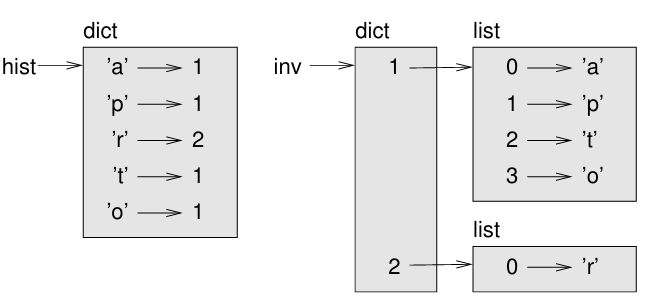
\includegraphics[width=0.7\linewidth]{images/chapter_11_1.png} % Ajusta el nombre del archivo
\caption{Diagrama de estado.}
\label{fig:diagrama_estado}
\end{figure}

Cada vez que pasa por el bucle, \texttt{key} obtiene una clave de \texttt{d} y \texttt{val} obtiene el valor correspondiente. Si \texttt{val} no está en \texttt{inverse}, significa que no lo hemos visto antes, por lo que creamos un nuevo ítem y lo inicializamos con un \textbf{singleton} (una lista que contiene un solo elemento). De lo contrario, hemos visto este valor antes, por lo que agregamos la clave correspondiente a la lista.

Aquí hay un ejemplo:

\begin{lstlisting}[language=Python]
>>> hist = histogram('parrot')
>>> hist
{'a': 1, 'p': 1, 'r': 2, 't': 1, 'o': 1}
>>> inverse = invert_dict(hist)
>>> inverse
{1: ['a', 'p', 't', 'o'], 2: ['r']}
\end{lstlisting}

Las listas pueden ser valores en un diccionario, como muestra este ejemplo, pero no pueden ser claves. Esto es lo que sucede si lo intentas:

\begin{lstlisting}[language=Python]
>>> t = [1, 2, 3]
>>> d = dict()
>>> d[t] = 'oops'
Traceback (most recent call last):
    File "<stdin>", line 1, in ?
TypeError: list objects are unhashable
\end{lstlisting}

Como mencioné antes, un diccionario se implementa usando una tabla hash, y eso significa que las claves deben ser \textbf{hashables}.

Un \textbf{hash} es una función que toma un valor (de cualquier tipo) y devuelve un entero. Los diccionarios usan estos enteros, llamados valores hash, para almacenar y buscar pares clave-valor.

Este sistema funciona bien si las claves son inmutables. Pero si las claves son mutables, como las listas, suceden cosas malas. Por ejemplo, cuando creas un par clave-valor, Python aplica el hash a la clave y la almacena en la ubicación correspondiente. Si modificas la clave y luego aplicas el hash nuevamente, iría a una ubicación diferente. En ese caso, podrías tener dos entradas para la misma clave, o podrías no poder encontrar una clave. De cualquier manera, el diccionario no funcionaría correctamente.

Por eso las claves deben ser hashables, y por qué tipos mutables como las listas no lo son. La forma más sencilla de evitar esta limitación es usar tuplas, que veremos en el próximo capítulo.

\begin{figure}[h]
\centering
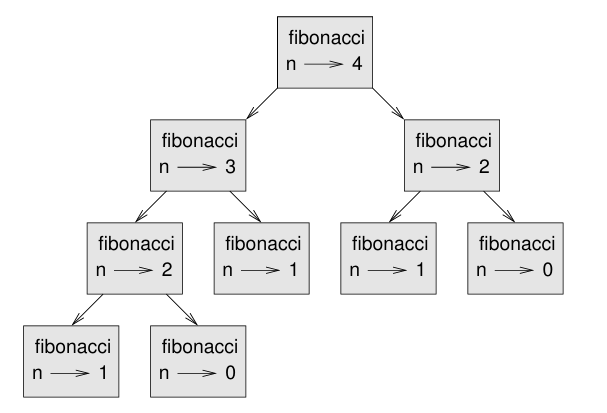
\includegraphics[width=0.7\linewidth]{images/chapter_11_2.png} % Ajusta el nombre del archivo
\caption{Gráfico de llamada.}
\label{fig:diagrama_estado}
\end{figure}

Dado que los diccionarios son mutables, no s epueden usar como claves, pero se pueden usar como valores.

\section{Memorización}

Si jugaste con la función \texttt{fibonacci} de la Sección 6.7, quizás hayas notado que cuanto más grande es el argumento que proporcionas, más tiempo tarda la función en ejecutarse. Además, el tiempo de ejecución aumenta rápidamente.

Para entender por qué, considera la Figura 11.2, que muestra el \textbf{gráfico de llamadas} para \texttt{fibonacci} con \texttt{n=4}:

Un gráfico de llamadas muestra un conjunto de marcos de función, con líneas que conectan cada marco con los marcos de las funciones que llama. En la parte superior del gráfico, \texttt{fibonacci} con \texttt{n=4} llama a \texttt{fibonacci} con \texttt{n=3} y \texttt{n=2}. A su vez, \texttt{fibonacci} con \texttt{n=3} llama a \texttt{fibonacci} con \texttt{n=2} y \texttt{n=1}. Y así sucesivamente.

Cuenta cuántas veces se llama a \texttt{fibonacci(0)} y \texttt{fibonacci(1)}. Esta es una solución ineficiente al problema, y empeora a medida que el argumento crece.

Una solución es hacer un seguimiento de los valores que ya se han calculado almacenándolos en un diccionario. Un valor previamente calculado que se almacena para su uso posterior se llama \textbf{memo}. Aquí hay una versión "memoizada" de \texttt{fibonacci}:

\begin{lstlisting}[language=Python]
known = {0:0, 1:1}

def fibonacci(n):
    if n in known:
        return known[n]
    res = fibonacci(n-1) + fibonacci(n-2)
    known[n] = res
    return res
\end{lstlisting}

\texttt{known} es un diccionario que lleva un registro de los números de Fibonacci que ya conocemos. Comienza con dos ítems: 0 mapea a 0 y 1 mapea a 1.

Cada vez que se llama a \texttt{fibonacci}, verifica \texttt{known}. Si el resultado ya está allí, puede devolverlo inmediatamente. De lo contrario, tiene que calcular el nuevo valor, agregarlo al diccionario y devolverlo.

Si ejecutas esta versión de \texttt{fibonacci} y la comparas con la original, encontrarás que es mucho más rápida.

\section{Glosario}

\begin{description}
    \item[mapeo:] Una relación en la que cada elemento de un conjunto corresponde a un elemento de otro conjunto.
    \item[diccionario:] Un mapeo de claves a sus valores correspondientes.
    \item[par clave-valor:] La representación del mapeo de una clave a un valor.
    \item[ítem:] En un diccionario, otro nombre para un par clave-valor.
    \item[clave:] Un objeto que aparece en un diccionario como la primera parte de un par clave-valor.
    \item[valor:] Un objeto que aparece en un diccionario como la segunda parte de un par clave-valor. Esto es más específico que nuestro uso anterior de la palabra "valor".
    \item[implementación:] Una forma de realizar un cálculo.
    \item[tabla hash:] El algoritmo utilizado para implementar los diccionarios de Python.
    \item[función hash:] Una función utilizada por una tabla hash para calcular la ubicación de una clave.
    \item[hashable:] Un tipo que tiene una función hash. Los tipos inmutables como enteros, flotantes y cadenas son hashables; los tipos mutables como listas y diccionarios no lo son.
    \item[búsqueda:] Una operación de diccionario que toma una clave y encuentra el valor correspondiente.
    \item[búsqueda inversa:] Una operación de diccionario que toma un valor y encuentra una o más claves que mapean a él.
    \item[sentencia raise:] Una sentencia que (deliberadamente) genera una excepción.
    \item[singleton:] Una lista (u otra secuencia) con un solo elemento.
    \item[gráfico de llamadas:] Un diagrama que muestra cada marco creado durante la ejecución de un programa, con una flecha de cada llamador a cada llamado.
    \item[memo:] Un valor calculado almacenado para evitar cálculos innecesarios en el futuro.
    \item[variable global:] Una variable definida fuera de una función. Las variables globales pueden ser accedidas desde cualquier función.
    \item[sentencia global:] Una sentencia que declara un nombre de variable global.
    \item[bandera:] Una variable booleana utilizada para indicar si una condición es verdadera.
    \item[declaración:] Una sentencia como \texttt{global} que le dice al intérprete algo sobre una variable.
\end{description}
%chapter 12

\chapter{Tuplas}

Este capítulo presenta otro tipo incorporado, la tupla, y luego muestra cómo las listas, los diccionarios y las tuplas trabajan juntos. También se presenta una característica útil para listas de argumentos de longitud variable: los operadores de reunión y dispersión.

Una nota: no hay consenso sobre cómo pronunciar "tuple". Algunas personas dicen "tú-pl", que rima con "sú-pl". Pero en el contexto de programación, la mayoría dice "tu-ple", que rima con "cuádruple".

\section{Las tuplas son inmutables}

Una tupla es una secuencia de valores. Los valores pueden ser de cualquier tipo y están indexados por enteros, por lo que en ese aspecto las tuplas son muy similares a las listas. La diferencia importante es que las tuplas son inmutables.

Sintácticamente, una tupla es una lista de valores separados por comas:

\begin{lstlisting}[language=Python]
>>> t = 'a', 'b', 'c', 'd', 'e'
\end{lstlisting}

Aunque no es necesario, es común encerrar las tuplas entre paréntesis:

\begin{lstlisting}[language=Python]
>>> t = ('a', 'b', 'c', 'd', 'e')
\end{lstlisting}

Para crear una tupla con un solo elemento, debes incluir una coma final:

\begin{lstlisting}[language=Python]
>>> t1 = 'a',
>>> type(t1)
<class 'tuple'>
\end{lstlisting}

Un valor entre paréntesis no es una tupla:

\begin{lstlisting}[language=Python]
>>> t2 = ('a')
>>> type(t2)
<class 'str'>
\end{lstlisting}

Otra forma de crear una tupla es usando la función incorporada \texttt{tuple}. Sin argumentos, crea una tupla vacía:

\begin{lstlisting}[language=Python]
>>> t = tuple()
>>> t
()
\end{lstlisting}

Si el argumento es una secuencia (cadena, lista o tupla), el resultado es una tupla con los elementos de la secuencia:

\begin{lstlisting}[language=Python]
>>> t = tuple('lupins')
>>> t
('l', 'u', 'p', 'i', 'n', 's')
\end{lstlisting}

Como \texttt{tuple} es el nombre de una función incorporada, debes evitar usarlo como nombre de variable.

La mayoría de los operadores de listas también funcionan con tuplas. El operador corchete indexa un elemento:

\begin{lstlisting}[language=Python]
>>> t = ('a', 'b', 'c', 'd', 'e')
>>> t[0]
'a'
\end{lstlisting}

Y el operador de segmento selecciona un rango de elementos:

\begin{lstlisting}[language=Python]
>>> t[1:3]
('b', 'c')
\end{lstlisting}

Pero si intentas modificar uno de los elementos de la tupla, obtendrás un error:

\begin{lstlisting}[language=Python]
>>> t[0] = 'A'
TypeError: object doesn't support item assignment
\end{lstlisting}

Como las tuplas son inmutables, no puedes modificar sus elementos. Pero puedes reemplazar una tupla por otra:

\begin{lstlisting}[language=Python]
>>> t = ('A',) + t[1:]
>>> t
('A', 'b', 'c', 'd', 'e')
\end{lstlisting}

Los operadores relacionales funcionan con tuplas y otras secuencias; Python comienza comparando el primer elemento de cada secuencia. Si son iguales, pasa a los siguientes elementos, y así sucesivamente, hasta encontrar elementos que difieran. Los elementos posteriores no se consideran (incluso si son muy grandes):

\begin{lstlisting}[language=Python]
>>> (0, 1, 2) < (0, 3, 4)
True
>>> (0, 1, 2000000) < (0, 3, 4)
True
\end{lstlisting}

\section{Asignación de tuplas}

A menudo es útil intercambiar los valores de dos variables. Con asignaciones convencionales, debes usar una variable temporal. Por ejemplo, para intercambiar \texttt{a} y \texttt{b}:

\begin{lstlisting}[language=Python]
>>> temp = a
>>> a = b
>>> b = temp
\end{lstlisting}

Esta solución es engorrosa; la asignación de tuplas es más elegante:

\begin{lstlisting}[language=Python]
>>> a, b = b, a
\end{lstlisting}

El lado izquierdo es una tupla de variables; el lado derecho es una tupla de expresiones. Cada valor se asigna a su respectiva variable. Todas las expresiones del lado derecho se evalúan antes de cualquier asignación.

El número de variables a la izquierda y el número de valores a la derecha deben ser iguales:

\begin{lstlisting}[language=Python]
>>> a, b = 1, 2, 3
ValueError: too many values to unpack
\end{lstlisting}

En general, el lado derecho puede ser cualquier tipo de secuencia (cadena, lista o tupla). Por ejemplo, para dividir una dirección de correo electrónico en un nombre de usuario y un dominio, podrías escribir:

\begin{lstlisting}[language=Python]
>>> addr = 'monty@python.org'
>>> uname, domain = addr.split('@')
\end{lstlisting}

El valor de retorno de \texttt{split} es una lista con dos elementos; el primer elemento se asigna a \texttt{uname}, el segundo a \texttt{domain}:

\begin{lstlisting}[language=Python]
>>> uname
'monty'
>>> domain
'python.org'
\end{lstlisting}

\section{Tuplas como valores de retorno}

Estrictamente hablando, una función solo puede devolver un valor, pero si el valor es una tupla, el efecto es el mismo que devolver múltiples valores. Por ejemplo, si quieres dividir dos enteros y calcular el cociente y el resto, es ineficiente calcular \texttt{x//y} y luego \texttt{x\%y}. Es mejor calcular ambos al mismo tiempo.

La función incorporada \texttt{divmod} toma dos argumentos y devuelve una tupla de dos valores, el cociente y el resto. Puedes almacenar el resultado como una tupla:

\begin{lstlisting}[language=Python]
>>> t = divmod(7, 3)
>>> t
(2, 1)
\end{lstlisting}

O usar asignación de tuplas para almacenar los elementos por separado:

\begin{lstlisting}[language=Python]
>>> quot, rem = divmod(7, 3)
>>> quot
2
>>> rem
1
\end{lstlisting}

Aquí hay un ejemplo de una función que devuelve una tupla:

\begin{lstlisting}[language=Python]
def min_max(t):
    return min(t), max(t)
\end{lstlisting}

\texttt{max} y \texttt{min} son funciones incorporadas que encuentran los elementos más grandes y más pequeños de una secuencia. \texttt{min\_max} calcula ambos y devuelve una tupla de dos valores.

\section{Tuplas de argumentos de longitud variable}

Las funciones pueden tomar un número variable de argumentos. Un nombre de parámetro que comienza con \texttt{*} recoge los argumentos en una tupla. Por ejemplo, \texttt{printall} toma cualquier número de argumentos y los imprime:

\begin{lstlisting}[language=Python]
def printall(*args):
    print(args)
\end{lstlisting}

El parámetro de recolección puede tener cualquier nombre, pero \texttt{args} es convencional. Así funciona la función:

\begin{lstlisting}[language=Python]
>>> printall(1, 2.0, '3')
(1, 2.0, '3')
\end{lstlisting}

El complemento de recolección es dispersión. Si tienes una secuencia de valores y quieres pasarla a una función como múltiples argumentos, puedes usar el operador \texttt{*}. Por ejemplo, \texttt{divmod} toma exactamente dos argumentos; no funciona con una tupla:

\begin{lstlisting}[language=Python]
>>> t = (7, 3)
>>> divmod(t)
TypeError: divmod expected 2 arguments, got 1
\end{lstlisting}

Pero si dispersas la tupla, funciona:

\begin{lstlisting}[language=Python]
>>> divmod(*t)
(2, 1)
\end{lstlisting}

Muchas funciones incorporadas usan tuplas de argumentos de longitud variable. Por ejemplo, \texttt{max} y \texttt{min} pueden tomar cualquier número de argumentos:

\begin{lstlisting}[language=Python]
>>> max(1, 2, 3)
3
\end{lstlisting}

Pero \texttt{sum} no:

\begin{lstlisting}[language=Python]
>>> sum(1, 2, 3)
TypeError: sum expected at most 2 arguments, got 3
\end{lstlisting}

Como ejercicio, escribe una función llamada \texttt{sum\_all} que tome cualquier número de argumentos y devuelva su suma.

\section{Listas y tuplas}

\texttt{zip} es una función incorporada que toma dos o más secuencias y las entrelaza. El nombre de la función se refiere a una cremallera, que entrelaza dos filas de dientes.

Este ejemplo entrelaza una cadena y una lista:

\begin{lstlisting}[language=Python]
>>> s = 'abc'
>>> t = [0, 1, 2]
>>> zip(s, t)
<zip object at 0x7f7d0a9e7c48>
\end{lstlisting}

El resultado es un objeto \texttt{zip} que sabe cómo iterar a través de los pares. El uso más común de \texttt{zip} es en un bucle \texttt{for}:

\begin{lstlisting}[language=Python]
>>> for pair in zip(s, t):
...     print(pair)
...
('a', 0)
('b', 1)
('c', 2)
\end{lstlisting}

Un objeto \texttt{zip} es un tipo de iterador, que es cualquier objeto que itera a través de una secuencia. Los iteradores son similares a las listas en algunos aspectos, pero a diferencia de las listas, no puedes usar un índice para seleccionar un elemento de un iterador.

Si quieres usar operadores y métodos de listas, puedes usar un objeto \texttt{zip} para crear una lista:

\begin{lstlisting}[language=Python]
>>> list(zip(s, t))
[('a', 0), ('b', 1), ('c', 2)]
\end{lstlisting}

El resultado es una lista de tuplas; en este ejemplo, cada tupla contiene un carácter de la cadena y el elemento correspondiente de la lista.

Si las secuencias no tienen la misma longitud, el resultado tiene la longitud de la más corta:

\begin{lstlisting}[language=Python]
>>> list(zip('Anne', 'Elk'))
[('A', 'E'), ('n', 'l'), ('n', 'k')]
\end{lstlisting}

Puedes usar asignación de tuplas en un bucle \texttt{for} para recorrer una lista de tuplas:

\begin{lstlisting}[language=Python]
t = [('a', 0), ('b', 1), ('c', 2)]
for letter, number in t:
    print(number, letter)
\end{lstlisting}

Cada vez que se recorre el bucle, Python selecciona la siguiente tupla en la lista y asigna los elementos a \texttt{letter} y \texttt{number}. La salida de este bucle es:

\begin{lstlisting}[language=Python]
0 a
1 b
2 c
\end{lstlisting}

Si combinas \texttt{zip}, \texttt{for} y asignación de tuplas, obtienes un patrón útil para recorrer dos (o más) secuencias al mismo tiempo. Por ejemplo, \texttt{has\_match} toma dos secuencias, \texttt{t1} y \texttt{t2}, y devuelve \texttt{True} si hay un índice \texttt{i} tal que \texttt{t1[i] == t2[i]}:

\begin{lstlisting}[language=Python]
def has_match(t1, t2):
    for x, y in zip(t1, t2):
        if x == y:
            return True
    return False
\end{lstlisting}

Si necesitas recorrer los elementos de una secuencia y sus índices, puedes usar la función incorporada \texttt{enumerate}:

\begin{lstlisting}[language=Python]
for index, element in enumerate('abc'):
    print(index, element)
\end{lstlisting}

El resultado de \texttt{enumerate} es un objeto \texttt{enumerate}, que itera una secuencia de pares; cada par contiene un índice (comenzando desde 0) y un elemento de la secuencia dada. En este ejemplo, la salida es:

\begin{lstlisting}[language=Python]
0 a
1 b
2 c
\end{lstlisting}

\section{Diccionarios y tuplas}

Los diccionarios tienen un método llamado \texttt{items} que devuelve una secuencia de tuplas, donde cada tupla es un par clave-valor.

\begin{lstlisting}[language=Python]
>>> d = {'a':0, 'b':1, 'c':2}
>>> t = d.items()
>>> t
dict_items([('c', 2), ('a', 0), ('b', 1)])
\end{lstlisting}

El resultado es un objeto \texttt{dict\_items}, que es un iterador que recorre los pares clave-valor. Puedes usarlo en un bucle \texttt{for} así:

\begin{lstlisting}[language=Python]
>>> for key, value in d.items():
...     print(key, value)
...
c 2
a 0
b 1
\end{lstlisting}

Como es de esperar en un diccionario, los elementos no tienen un orden particular.

En la otra dirección, puedes usar una lista de tuplas para inicializar un nuevo diccionario:

\begin{lstlisting}[language=Python]
>>> t = [('a', 0), ('c', 2), ('b', 1)]
>>> d = dict(t)
>>> d
{'a': 0, 'c': 2, 'b': 1}
\end{lstlisting}

Combinar \texttt{dict} con \texttt{zip} proporciona una forma concisa de crear un diccionario:

\begin{lstlisting}[language=Python]
>>> d = dict(zip('abc', range(3)))
>>> d
{'a': 0, 'c': 2, 'b': 1}
\end{lstlisting}

El método \texttt{update} de los diccionarios también toma una lista de tuplas y las agrega, como pares clave-valor, a un diccionario existente.

Es común usar tuplas como claves en diccionarios (principalmente porque no puedes usar listas). Por ejemplo, un directorio telefónico podría mapear pares apellido, nombre a números de teléfono. Suponiendo que hemos definido \texttt{last}, \texttt{first} y \texttt{number}, podríamos escribir:

\begin{lstlisting}[language=Python]
directory[last, first] = number
\end{lstlisting}

La expresión entre corchetes es una tupla. Podríamos usar asignación de tuplas para recorrer este diccionario:

\begin{lstlisting}[language=Python]
for last, first in directory:
    print(first, last, directory[last, first])
\end{lstlisting}

Este bucle recorre las claves en \texttt{directory}, que son tuplas. Asigna los elementos de cada tupla a \texttt{last} y \texttt{first}, luego imprime el nombre y el número de teléfono correspondiente.

Hay dos formas de representar tuplas en un diagrama de estado. La versión más detallada muestra los índices y elementos como aparecen en una lista. Por ejemplo, la tupla \texttt{('Cleese', 'John')} aparecería como en la Figura 12.1.

Pero en un diagrama más grande podrías omitir los detalles. Por ejemplo, un diagrama del directorio telefónico podría aparecer como en la Figura 12.2.

Aquí las tuplas se muestran usando la sintaxis de Python como una abreviatura gráfica. El número de teléfono en el diagrama es la línea de quejas de la BBC, así que por favor no lo llames.

\begin{figure}[h]
        \centering
        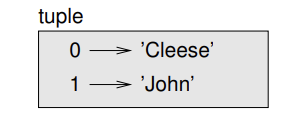
\includegraphics[width=0.5\textwidth]{./images/chapter_12_1.png}
        \caption{Diagrama de estados.}
        \label{fig:12_1}
        \end{figure}
        
\begin{figure}[h]
        \centering
        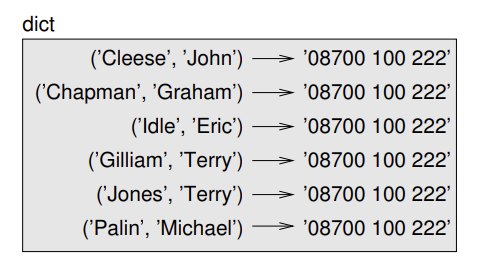
\includegraphics[width=0.5\textwidth]{./images/chapter_12_2.png}
        \caption{Diagrama de estados.}
        \label{fig:12_2}
        \end{figure}

\section{Secuencias de secuencias}

Me he centrado en listas de tuplas, pero casi todos los ejemplos de este capítulo también funcionan con listas de listas, tuplas de tuplas y tuplas de listas. Para evitar enumerar las posibles combinaciones, a veces es más fácil hablar de secuencias de secuencias.

En muchos contextos, los diferentes tipos de secuencias (cadenas, listas y tuplas) pueden usarse indistintamente. Entonces, ¿cómo elegir una sobre las otras?

Para empezar por lo obvio, las cadenas son más limitadas que otras secuencias porque los elementos tienen que ser caracteres. También son inmutables. Si necesitas la capacidad de cambiar los caracteres en una cadena (en lugar de crear una nueva cadena), podrías usar una lista de caracteres.

Las listas son más comunes que las tuplas, principalmente porque son mutables. Pero hay algunos casos donde podrías preferir tuplas:

1. En algunos contextos, como una sentencia \texttt{return}, es sintácticamente más simple crear una tupla que una lista.

2. Si quieres usar una secuencia como clave de diccionario, debes usar un tipo inmutable como una tupla o una cadena.

3. Si estás pasando una secuencia como argumento a una función, usar tuplas reduce el potencial de comportamientos inesperados debido a aliasing.

Como las tuplas son inmutables, no proporcionan métodos como \texttt{sort} y \texttt{reverse}, que modifican listas existentes. Pero Python proporciona la función incorporada \texttt{sorted}, que toma cualquier secuencia y devuelve una nueva lista con los mismos elementos en orden ordenado, y \texttt{reversed}, que toma una secuencia y devuelve un iterador que recorre la lista en orden inverso.

\section{Depuración}

Las listas, diccionarios y tuplas son ejemplos de estructuras de datos; en este capítulo estamos empezando a ver estructuras de datos compuestas, como listas de tuplas, o diccionarios que contienen tuplas como claves y listas como valores. Las estructuras de datos compuestas son útiles, pero son propensas a lo que llamo errores de forma; es decir, errores causados cuando una estructura de datos tiene el tipo, tamaño o estructura incorrectos. Por ejemplo, si esperas una lista con un entero y te doy un entero simple (no en una lista), no funcionará.

Para ayudar a depurar este tipo de errores, he escrito un módulo llamado \texttt{structshape} que proporciona una función, también llamada \texttt{structshape}, que toma cualquier tipo de estructura de datos como argumento y devuelve una cadena que resume su forma. Puedes descargarlo desde \url{https://thinkpython.com/code/structshape.py}

Aquí está el resultado para una lista simple:

\begin{lstlisting}[language=Python]
>>> from structshape import structshape
>>> t = [1, 2, 3]
>>> structshape(t)
'list of 3 int'
\end{lstlisting}

Un programa más elegante podría escribir "list of 3 ints", pero era más fácil no lidiar con plurales. Aquí hay una lista de listas:

\begin{lstlisting}[language=Python]
>>> t2 = [[1,2], [3,4], [5,6]]
>>> structshape(t2)
'list of 3 list of 2 int'
\end{lstlisting}

Si los elementos de la lista no son del mismo tipo, \texttt{structshape} los agrupa, en orden, por tipo:

\begin{lstlisting}[language=Python]
>>> t3 = [1, 2, 3, 4.0, '5', '6', [7], [8], 9]
>>> structshape(t3)
'list of (3 int, float, 2 str, 2 list of int, int)'
\end{lstlisting}

Aquí hay una lista de tuplas:

\begin{lstlisting}[language=Python]
>>> s = 'abc'
>>> lt = list(zip(t, s))
>>> structshape(lt)
'list of 3 tuple of (int, str)'
\end{lstlisting}

Y aquí hay un diccionario con 3 elementos que mapean enteros a cadenas:

\begin{lstlisting}[language=Python]
>>> d = dict(lt)
>>> structshape(d)
'dict of 3 int->str'
\end{lstlisting}

Si tienes problemas para mantener el seguimiento de tus estructuras de datos, \texttt{structshape} puede ayudarte.

\section{Glosario}

\begin{description}
\item[tupla:] Una secuencia inmutable de elementos.

\item[asignación de tuplas:] Una asignación con una secuencia en el lado derecho y una tupla de variables en el izquierdo. El lado derecho se evalúa y luego sus elementos se asignan a las variables de la izquierda.

\item[recolección:] Una operación que recoge múltiples argumentos en una tupla.

\item[dispersión:] Una operación que hace que una secuencia se comporte como múltiples argumentos.

\item[objeto zip:] El resultado de llamar a la función incorporada \texttt{zip}; un objeto que itera a través de una secuencia de tuplas.

\item[iterador:] Un objeto que puede iterar a través de una secuencia, pero que no proporciona operadores y métodos de listas.

\item[estructura de datos:] Una colección de valores relacionados, a menudo organizados en listas, diccionarios, tuplas, etc.

\item[error de forma:] Un error causado porque un valor tiene la forma incorrecta; es decir, el tipo o tamaño incorrecto.
\end{description}

\section{Ejercicios}

\textbf{Ejercicio 12.1.} Escribe una función llamada \texttt{most\_frequent} que tome una cadena e imprima las letras en orden decreciente de frecuencia. Encuentra muestras de texto en varios idiomas diferentes y observa cómo varía la frecuencia de las letras entre idiomas. Compara tus resultados con las tablas en \url{http://en.wikipedia.org/wiki/Letter_frequencies}. Solución: \url{https://thinkpython.com/code/most_frequent.py}.

\textbf{Ejercicio 12.2.} ¡Más anagramas!

1. Escribe un programa que lea una lista de palabras de un archivo (ver Sección 9.1) e imprima todos los conjuntos de palabras que son anagramas. Aquí hay un ejemplo de cómo podría verse la salida:

\begin{lstlisting}[language=Python]
['deltas', 'desalt', 'lasted', 'salted', 'slated', 'staled']
['retainers', 'ternaries']
['generating', 'greatening']
['resmelts', 'smelters', 'termless']
\end{lstlisting}

Pista: podrías construir un diccionario que mapee desde una colección de letras a una lista de palabras que se pueden escribir con esas letras. La pregunta es, ¿cómo puedes representar la colección de letras de una manera que se pueda usar como clave?

2. Modifica el programa anterior para que imprima la lista más larga de anagramas primero, seguida de la segunda más larga, y así sucesivamente.

3. En Scrabble, un "bingo" es cuando juegas las siete fichas de tu soporte, junto con una letra en el tablero, para formar una palabra de ocho letras. ¿Qué colección de 8 letras forma la mayor cantidad de bingos posibles? Solución: \url{https://thinkpython.com/code/anagram_sets.py}.

\textbf{Ejercicio 12.3.} Dos palabras forman un "par de metátesis" si puedes transformar una en la otra intercambiando dos letras; por ejemplo, "converse" y "conserve". Escribe un programa que encuentre todos los pares de metátesis en el diccionario. Pista: no pruebes todos los pares de palabras, y no pruebes todos los intercambios posibles. Solución: \url{https://thinkpython.com/code/metathesis.py}. Crédito: Este ejercicio está inspirado en un ejemplo en \url{http://puzzlers.org}.

\textbf{Ejercicio 12.4.} Aquí hay otro Puzzler de Car Talk (\url{http://www.cartalk.com/content/puzzlers}):

¿Cuál es la palabra más larga en inglés que sigue siendo una palabra válida en inglés a medida que eliminas sus letras una a una? Ahora, las letras se pueden eliminar de cualquier extremo o del medio, pero no puedes reorganizar ninguna de las letras. Cada vez que eliminas una letra, terminas con otra palabra en inglés. Si haces eso, eventualmente terminarás con una letra, y esa también será una palabra en inglés, una que se encuentre en el diccionario. Quiero saber cuál es la palabra más larga y cuántas letras tiene. Voy a darte un pequeño ejemplo modesto: Sprite. ¿Ok? Comienzas con sprite, quitas una letra, una del interior de la palabra, quitas la r, y nos queda spite, luego quitamos la e del final, nos queda spit, quitamos la s, nos queda pit, it, e I.

Escribe un programa para encontrar todas las palabras que se pueden reducir de esta manera y luego encuentra la más larga.

Este ejercicio es un poco más desafiante que la mayoría, así que aquí hay algunas sugerencias:

1. Podrías escribir una función que tome una palabra y calcule una lista de todas las palabras que se pueden formar eliminando una letra. Estas son las "hijas" de la palabra.

2. Recursivamente, una palabra es reducible si cualquiera de sus hijas es reducible. Como caso base, puedes considerar la cadena vacía reducible.

3. La lista de palabras que proporcioné, \texttt{words.txt}, no contiene palabras de una sola letra. Así que podrías agregar "I", "a" y la cadena vacía.

4. Para mejorar el rendimiento de tu programa, podrías memorizar las palabras que se sabe que son reducibles.

Solución: \url{https://thinkpython.com/code/reducible.py}.
\chapter{Caso de estudio: selección de estructuras de datos}

En este punto has aprendido sobre las estructuras de datos principales de Python y has visto algunos algoritmos que las utilizan. Si deseas saber más sobre algoritmos, este podría ser un buen momento para leer el Capítulo B. Pero no es necesario que lo leas antes de continuar; puedes leerlo cuando te interese.

Este capítulo presenta un caso de estudio con ejercicios que te permitirán pensar sobre la selección de estructuras de datos y practicar su uso.

\section{Análisis de frecuencia de palabras}

Como siempre, deberías intentar resolver los ejercicios antes de leer mis soluciones.

\textbf{Ejercicio 13.1.} Escribe un programa que lea un archivo, divida cada línea en palabras, elimine los espacios en blanco y la puntuación de las palabras, y las convierta a minúsculas.

\textit{Sugerencia: El módulo \texttt{string} proporciona una cadena llamada \texttt{whitespace}, que contiene espacios, tabulaciones, saltos de línea, etc., y \texttt{punctuation} que contiene los caracteres de puntuación. Veamos si podemos hacer que Python "jure":}

\begin{lstlisting}[language=Python]
>>> import string
>>> string.punctuation
'!"#$%&\'()*+,-./:;<=>?@[\\]^_`{|}~'
\end{lstlisting}

\textit{Además, podrías considerar usar los métodos de cadena \texttt{strip}, \texttt{replace} y \texttt{translate}.}

\textbf{Ejercicio 13.2.} Ve a Project Gutenberg (\url{http://gutenberg.org}) y descarga tu libro favorito que esté libre de derechos de autor, en formato de texto plano.

\textit{Modifica tu programa del ejercicio anterior para leer el libro que descargaste, omitir la información del encabezado al principio del archivo y procesar el resto de las palabras como antes.}

\textit{Luego, modifica el programa para contar el número total de palabras en el libro y la cantidad de veces que aparece cada palabra.}

\textit{Imprime el número de palabras diferentes utilizadas en el libro. Compara libros de diferentes autores, escritos en diferentes épocas. ¿Qué autor utiliza el vocabulario más extenso?}

\textbf{Ejercicio 13.3.} Modifica el programa del ejercicio anterior para imprimir las 20 palabras más frecuentes en el libro.

\textbf{Ejercicio 13.4.} Modifica el programa anterior para leer una lista de palabras (ver Sección 9.1) y luego imprimir todas las palabras del libro que no estén en la lista de palabras. ¿Cuántas de ellas son errores tipográficos? ¿Cuántas son palabras comunes que deberían estar en la lista y cuántas son realmente oscuras?

\section{Números aleatorios}

Con las mismas entradas, la mayoría de los programas de computadora generan las mismas salidas cada vez, por lo que se dice que son \textbf{deterministas}. El determinismo suele ser algo bueno, ya que esperamos que el mismo cálculo produzca el mismo resultado. Sin embargo, para algunas aplicaciones queremos que la computadora sea impredecible. Los juegos son un ejemplo obvio, pero hay más.

Hacer que un programa sea verdaderamente no determinista es difícil, pero hay formas de hacer que al menos parezca no determinista. Una de ellas es usar algoritmos que generen números \textbf{pseudoaleatorios}. Estos números no son verdaderamente aleatorios porque se generan mediante un cálculo determinista, pero a simple vista es casi imposible distinguirlos de los aleatorios.

El módulo \texttt{random} proporciona funciones que generan números pseudoaleatorios (que simplemente llamaré "aleatorios" de ahora en adelante).

La función \texttt{random} devuelve un flotante aleatorio entre 0.0 y 1.0 (incluyendo 0.0 pero no 1.0). Cada vez que llamas a \texttt{random}, obtienes el siguiente número en una larga serie. Para ver un ejemplo, ejecuta este bucle:

\begin{lstlisting}[language=Python]
import random
for i in range(10):
    x = random.random()
    print(x)
\end{lstlisting}

La función \texttt{randint} toma los parámetros \texttt{low} y \texttt{high} y devuelve un entero entre \texttt{low} y \texttt{high} (incluyendo ambos).

\begin{lstlisting}[language=Python]
>>> random.randint(5, 10)
5
>>> random.randint(5, 10)
9
\end{lstlisting}

Para elegir un elemento de una secuencia al azar, puedes usar \texttt{choice}:

\begin{lstlisting}[language=Python]
>>> t = [1, 2, 3]
>>> random.choice(t)
2
>>> random.choice(t)
3
\end{lstlisting}

El módulo \texttt{random} también proporciona funciones para generar valores aleatorios a partir de distribuciones continuas, incluyendo Gaussianas, exponenciales, gamma y algunas más.

\textbf{Ejercicio 13.5.} Escribe una función llamada \texttt{choose\_from\_hist} que tome un histograma como se define en la Sección 11.2 y devuelva un valor aleatorio del histograma, elegido con una probabilidad proporcional a su frecuencia. Por ejemplo, para este histograma:

\begin{lstlisting}[language=Python]
>>> t = ['a', 'a', 'b']
>>> hist = histogram(t)
>>> hist
{'a': 2, 'b': 1}
\end{lstlisting}

tu función debería devolver \texttt{'a'} con probabilidad \(2/3\) y \texttt{'b'} con probabilidad \(1/3\).

\section{Histograma de palabras}

Deberías intentar los ejercicios anteriores antes de continuar. Puedes descargar mi solución desde \url{https://thinkpython.com/code/analyze_book1.py}. También necesitarás \url{https://thinkpython.com/code/emma.txt}.

Aquí hay un programa que lee un archivo y construye un histograma de las palabras en el archivo:

\begin{lstlisting}[language=Python]
import string

def process_file(filename):
    hist = dict()
    fp = open(filename)
    for line in fp:
        process_line(line, hist)
    return hist

def process_line(line, hist):
    line = line.replace('-', ' ')
    
    for word in line.split():
        word = word.strip(string.punctuation + string.whitespace)
        word = word.lower()
        hist[word] = hist.get(word, 0) + 1

hist = process_file('emma.txt')
\end{lstlisting}

Este programa lee \texttt{emma.txt}, que contiene el texto de \textit{Emma} de Jane Austen.

\texttt{process\_file} recorre las líneas del archivo, pasándolas una a una a \texttt{process\_line}. El histograma \texttt{hist} se utiliza como acumulador.

\texttt{process\_line} usa el método \texttt{replace} para reemplazar guiones con espacios antes de usar \texttt{split} para dividir la línea en una lista de cadenas. Luego recorre la lista de palabras y usa \texttt{strip} y \texttt{lower} para eliminar puntuación y convertir a minúsculas. (Es una forma abreviada de decir que las cadenas se "convierten"; recuerda que las cadenas son inmutables, por lo que métodos como \texttt{strip} y \texttt{lower} devuelven nuevas cadenas.)

Finalmente, \texttt{process\_line} actualiza el histograma creando un nuevo elemento o incrementando uno existente.

Para contar el número total de palabras en el archivo, podemos sumar las frecuencias en el histograma:

\begin{lstlisting}[language=Python]
def total_words(hist):
    return sum(hist.values())
\end{lstlisting}

El número de palabras diferentes es simplemente el número de elementos en el diccionario:

\begin{lstlisting}[language=Python]
def different_words(hist):
    return len(hist)
\end{lstlisting}

Aquí hay un código para imprimir los resultados:

\begin{lstlisting}[language=Python]
print('Total number of words:', total_words(hist))
print('Number of different words:', different_words(hist))
\end{lstlisting}

Y los resultados:

\begin{lstlisting}[language=Python]
Total number of words: 161080
Number of different words: 7214
\end{lstlisting}

\section{Palabras más comunes}

Para encontrar las palabras más comunes, podemos hacer una lista de tuplas, donde cada tupla contiene una palabra y su frecuencia, y ordenarla.

La siguiente función toma un histograma y devuelve una lista de tuplas palabra-frecuencia:

\begin{lstlisting}[language=Python]
def most_common(hist):
    t = []
    for key, value in hist.items():
        t.append((value, key))
    
    t.sort(reverse=True)
    return t
\end{lstlisting}

En cada tupla, la frecuencia aparece primero, por lo que la lista resultante está ordenada por frecuencia. Aquí hay un bucle que imprime las diez palabras más comunes:

\begin{lstlisting}[language=Python]
t = most_common(hist)
print('The most common words are:')
for freq, word in t[:10]:
    print(word, freq, sep='\t')
\end{lstlisting}

Uso el argumento de palabra clave \texttt{sep} para indicar a \texttt{print} que use un tabulador como "separador", en lugar de un espacio, para que la segunda columna quede alineada. Aquí están los resultados de \textit{Emma}:

\begin{lstlisting}[language=Python]
The most common words are:
to      5242
the     5205
and     4897
of      4295
i       3191
a       3130
it      2529
her     2483
was     2400
she     2364
\end{lstlisting}

Este código se puede simplificar usando el parámetro \texttt{key} de la función \texttt{sort}. Si tienes curiosidad, puedes leer sobre esto en \url{https://wiki.python.org/moin/HowTo/Sorting}.

\section{Parámetros opcionales}

Hemos visto funciones y métodos integrados que toman argumentos opcionales. También es posible escribir funciones definidas por el usuario con argumentos opcionales. Por ejemplo, aquí hay una función que imprime las palabras más comunes en un histograma:

\begin{lstlisting}[language=Python]
def print_most_common(hist, num=10):
    t = most_common(hist)
    print('The most common words are:')
    for freq, word in t[:num]:
        print(word, freq, sep='\t')
\end{lstlisting}

El primer parámetro es obligatorio; el segundo es opcional. El valor predeterminado de \texttt{num} es 10.

Si solo proporcionas un argumento:

\begin{lstlisting}[language=Python]
print_most_common(hist)
\end{lstlisting}

\texttt{num} toma el valor predeterminado. Si proporcionas dos argumentos:

\begin{lstlisting}[language=Python]
print_most_common(hist, 20)
\end{lstlisting}

\texttt{num} toma el valor del argumento. En otras palabras, el argumento opcional anula el valor predeterminado.

Si una función tiene parámetros obligatorios y opcionales, todos los obligatorios deben ir primero, seguidos de los opcionales.

\section{Resta de diccionarios}

Encontrar las palabras del libro que no están en la lista de palabras de \texttt{words.txt} es un problema que podrías reconocer como resta de conjuntos; es decir, queremos encontrar todas las palabras de un conjunto (las palabras del libro) que no están en el otro (las palabras de la lista).

\texttt{subtract} toma los diccionarios \texttt{d1} y \texttt{d2} y devuelve un nuevo diccionario que contiene todas las claves de \texttt{d1} que no están en \texttt{d2}. Como realmente no nos importan los valores, los establecemos todos en \texttt{None}.

\begin{lstlisting}[language=Python]
def subtract(d1, d2):
    res = dict()
    for key in d1:
        if key not in d2:
            res[key] = None
    return res
\end{lstlisting}

Para encontrar las palabras del libro que no están en \texttt{words.txt}, podemos usar \texttt{process\_file} para construir un histograma para \texttt{words.txt}, y luego restar:

\begin{lstlisting}[language=Python]
words = process_file('words.txt')
diff = subtract(hist, words)

print("Words in the book that aren't in the word list:")
for word in diff:
    print(word, end=' ')
\end{lstlisting}

Aquí están algunos de los resultados de \textit{Emma}:

\begin{lstlisting}[language=Python]
Words in the book that aren't in the word list:
rencontre jane's blanche woodhouses disingenuousness friend's venice apartment ...
\end{lstlisting}

Algunas de estas palabras son nombres y posesivos. Otras, como "rencontre", ya no son de uso común. ¡Pero algunas son palabras comunes que realmente deberían estar en la lista!

\textbf{Ejercicio 13.6.} Python proporciona una estructura de datos llamada \texttt{set} que ofrece muchas operaciones comunes de conjuntos. Puedes leer sobre ellas en la Sección 19.5 o en la documentación en \url{http://docs.python.org/3/library/stdtypes.html#types-set}.

\textit{Escribe un programa que use resta de conjuntos para encontrar palabras en el libro que no están en la lista de palabras. Solución: \url{https://thinkpython.com/code/analyze_book3.py}.}

\section{Palabras aleatorias}

Para elegir una palabra aleatoria del histograma, el algoritmo más simple es construir una lista con múltiples copias de cada palabra, según la frecuencia observada, y luego elegir de la lista:

\begin{lstlisting}[language=Python]
def random_word(h):
    t = []
    for word, freq in h.items():
        t.extend([word] * freq)
    return random.choice(t)
\end{lstlisting}

La expresión \texttt{[word] * freq} crea una lista con \texttt{freq} copias de la cadena \texttt{word}. El método \texttt{extend} es similar a \texttt{append}, excepto que el argumento es una secuencia.

Este algoritmo funciona, pero no es muy eficiente; cada vez que eliges una palabra aleatoria, reconstruye la lista, que es tan grande como el libro original. Una mejora obvia es construir la lista una vez y luego hacer múltiples selecciones, pero la lista sigue siendo grande.

Una alternativa es:

1. Usar \texttt{keys} para obtener una lista de las palabras en el libro.

2. Construir una lista que contenga la suma acumulativa de las frecuencias de las palabras (ver Ejercicio 10.2). El último elemento de esta lista es el número total de palabras en el libro, \(n\).

3. Elegir un número aleatorio entre 1 y \(n\). Usar una búsqueda por bisección (ver Ejercicio 10.10) para encontrar el índice donde se insertaría el número aleatorio en la suma acumulativa.

4. Usar el índice para encontrar la palabra correspondiente en la lista de palabras.

\textbf{Ejercicio 13.7.} \textit{Escribe un programa que use este algoritmo para elegir una palabra aleatoria del libro. Solución: \url{https://thinkpython.com/code/analyze_book3.py}.}

\section{Análisis de Markov}

Si eliges palabras del libro al azar, puedes tener una idea del vocabulario, pero probablemente no obtendrás una oración:

\begin{lstlisting}[language=Python]
this the small regard harriet which knightley's it most things
\end{lstlisting}

Una serie de palabras aleatorias rara vez tiene sentido porque no hay relación entre palabras sucesivas. Por ejemplo, en una oración real, esperarías que un artículo como "the" fuera seguido por un adjetivo o un sustantivo, y probablemente no por un verbo o adverbio.

Una forma de medir este tipo de relaciones es el \textbf{análisis de Markov}, que caracteriza, para una secuencia dada de palabras, la probabilidad de las palabras que podrían venir a continuación. Por ejemplo, la canción \textit{Eric, the Half a Bee} comienza:

\begin{quote}
Half a bee, philosophically,\\
Must, ipso facto, half not be.\\
But half the bee has got to be\\
Vis a vis, its entity. D'you see?\\
\\
But can a bee be said to be\\
Or not to be an entire bee\\
When half the bee is not a bee\\
Due to some ancient injury?
\end{quote}

En este texto, la frase "half the" siempre es seguida por la palabra "bee", pero la frase "the bee" podría ser seguida por "has" o "is".

El resultado del análisis de Markov es una correspondencia entre cada prefijo (como "half the" o "the bee") y todos sus posibles sufijos (como "has" e "is").

A partir de este mapeo, puedes generar un texto aleatorio comenzando con cualquier prefijo y eligiendo aleatoriamente uno de los sufijos asociados. Luego, puedes combinar la última palabra del prefijo con el sufijo elegido para formar un nuevo prefijo, y repetir el proceso.

Por ejemplo, si comienzas con el prefijo "Half a", la siguiente palabra debe ser "bee", ya que ese prefijo solo aparece una vez en el texto. El nuevo prefijo será entonces "a bee", por lo que el siguiente sufijo podría ser "philosophically", "be" o "due".

En este ejemplo, la longitud del prefijo es siempre dos, pero puedes realizar un análisis de Markov con cualquier longitud de prefijo.

\textbf{Ejercicio 13.8.} Análisis de Markov:

1. Escribe un programa para leer un texto desde un archivo y realizar un análisis de Markov. El resultado debería ser un diccionario que mapee desde prefijos a una colección de sufijos posibles. La colección podría ser una lista, tupla o diccionario; depende de ti elegir la opción apropiada. Puedes probar tu programa con una longitud de prefijo dos, pero deberías escribir el programa de manera que sea fácil probar otras longitudes.

2. Agrega una función al programa anterior para generar texto aleatorio basado en el análisis de Markov. Aquí hay un ejemplo de \textit{Emma} con longitud de prefijo 2:

\begin{quote}
He was very clever, be it sweetness or be angry, ashamed or only amused, at such a stroke. She had never thought of Hannah till you were never meant for me? "I cannot make speeches, Emma:" he soon cut it all himself.
\end{quote}

Para este ejemplo, dejé la puntuación unida a las palabras. El resultado es casi sintácticamente correcto, pero no del todo. Semánticamente, casi tiene sentido, pero no completamente.

¿Qué sucede si aumentas la longitud del prefijo? ¿El texto aleatorio tiene más sentido?

3. Una vez que tu programa funcione, podrías probar una mezcla: si combinas texto de dos o más libros, el texto aleatorio que generes mezclará el vocabulario y las frases de las fuentes de manera interesante.

\textit{Crédito: Este caso de estudio está basado en un ejemplo de Kernighan y Pike, \textit{The Practice of Programming}, Addison-Wesley, 1999.}

Deberías intentar este ejercicio antes de continuar; luego puedes descargar mi solución desde \url{https://thinkpython.com/code/markov.py}. También necesitarás \url{https://thinkpython.com/code/emma.txt}.

\section{Estructuras de datos}

Usar análisis de Markov para generar texto aleatorio es divertido, pero también hay un propósito en este ejercicio: la selección de estructuras de datos. En tu solución a los ejercicios anteriores, tuviste que elegir:

\begin{itemize}
    \item Cómo representar los prefijos.
    \item Cómo representar la colección de sufijos posibles.
    \item Cómo representar el mapeo desde cada prefijo a la colección de sufijos posibles.
\end{itemize}

El último es fácil: un diccionario es la opción obvia para un mapeo de claves a valores correspondientes.

Para los prefijos, las opciones más obvias son cadena, lista de cadenas o tupla de cadenas.

Para los sufijos, una opción es una lista; otra es un histograma (diccionario).

¿Cómo elegir? El primer paso es pensar en las operaciones que necesitarás implementar para cada estructura de datos. Para los prefijos, necesitamos poder eliminar palabras del principio y agregar al final. Por ejemplo, si el prefijo actual es "Half a", y la siguiente palabra es "bee", necesitas poder formar el siguiente prefijo, "a bee".

Tu primera elección podría ser una lista, ya que es fácil agregar y eliminar elementos, pero también necesitamos poder usar los prefijos como claves en un diccionario, lo que descarta las listas. Con las tuplas, no puedes agregar o eliminar, pero puedes usar el operador de suma para formar una nueva tupla:

\begin{lstlisting}[language=Python]
def shift(prefix, word):
    return prefix[1:] + (word,)
\end{lstlisting}

\texttt{shift} toma una tupla de palabras, \texttt{prefix}, y una cadena, \texttt{word}, y forma una nueva tupla que tiene todas las palabras en \texttt{prefix} excepto la primera, y \texttt{word} agregada al final.

Para la colección de sufijos, las operaciones que necesitamos realizar incluyen agregar un nuevo sufijo (o incrementar la frecuencia de uno existente) y elegir un sufijo aleatorio.

Agregar un nuevo sufijo es igual de fácil para la implementación de lista o histograma. Elegir un elemento aleatorio de una lista es fácil; elegir de un histograma es más difícil de hacer eficientemente (ver Ejercicio 13.7).

Hasta ahora hemos estado hablando principalmente sobre la facilidad de implementación, pero hay otros factores a considerar al elegir estructuras de datos. Uno es el tiempo de ejecución. A veces hay una razón teórica para esperar que una estructura de datos sea más rápida que otra; por ejemplo, mencioné que el operador \texttt{in} es más rápido para diccionarios que para listas, al menos cuando el número de elementos es grande.

Pero a menudo no sabes de antemano cuál implementación será más rápida. Una opción es implementar ambas y ver cuál es mejor. Este enfoque se llama \textbf{benchmarking}. Una alternativa práctica es elegir la estructura de datos más fácil de implementar y ver si es lo suficientemente rápida para la aplicación prevista. Si es así, no hay necesidad de continuar. Si no, hay herramientas, como el módulo \texttt{profile}, que pueden identificar las partes de un programa que consumen más tiempo.

El otro factor a considerar es el espacio de almacenamiento. Por ejemplo, usar un histograma para la colección de sufijos podría tomar menos espacio porque solo tienes que almacenar cada palabra una vez, sin importar cuántas veces aparezca en el texto. En algunos casos, ahorrar espacio también puede hacer que tu programa se ejecute más rápido, y en casos extremos, tu programa podría no ejecutarse si se queda sin memoria. Pero para muchas aplicaciones, el espacio es una consideración secundaria después del tiempo de ejecución.

Un pensamiento final: en esta discusión, he implicado que deberíamos usar una estructura de datos tanto para el análisis como para la generación. Pero como estas son fases separadas, también sería posible usar una estructura para el análisis y luego convertir a otra estructura para la generación. Esto sería una ganancia neta si el tiempo ahorrado durante la generación superara el tiempo gastado en la conversión.

\section{Depuración}

Cuando estás depurando un programa, y especialmente si estás trabajando en un error difícil, hay cinco cosas que probar:

\begin{itemize}
    \item \textbf{Leer:} Examina tu código, léelo en voz alta y verifica que diga lo que pretendías.
    
    \item \textbf{Ejecutar:} Experimenta haciendo cambios y ejecutando diferentes versiones. A menudo, si muestras lo correcto en el lugar correcto del programa, el problema se vuelve obvio, pero a veces tienes que construir andamiaje.
    
    \item \textbf{Reflexionar:} ¡Tómate un tiempo para pensar! ¿Qué tipo de error es: sintaxis, tiempo de ejecución o semántico? ¿Qué información puedes obtener de los mensajes de error o de la salida del programa? ¿Qué tipo de error podría causar el problema que estás viendo? ¿Qué cambiaste justo antes de que apareciera el problema?
    
    \item \textbf{Explicar:} Si le explicas el problema a alguien más, a veces encuentras la respuesta antes de terminar de hacer la pregunta. A menudo no necesitas a la otra persona; podrías hablarle a un pato de goma. Y ese es el origen de la conocida estrategia llamada \textbf{depuración con pato de goma}. No estoy inventando esto; ver \url{https://en.wikipedia.org/wiki/Rubber_duck_debugging}.
    
    \item \textbf{Retroceder:} En algún momento, lo mejor es retroceder, deshaciendo cambios recientes, hasta volver a un programa que funcione y que entiendas. Luego puedes comenzar a reconstruir.
\end{itemize}

Los programadores principiantes a veces se estancan en una de estas actividades y olvidan las demás. Cada actividad viene con su propio modo de fallo.

Por ejemplo, leer tu código podría ayudar si el problema es un error tipográfico, pero no si el problema es un malentendido conceptual. Si no entiendes lo que hace tu programa, puedes leerlo 100 veces y nunca ver el error, porque el error está en tu cabeza.

Ejecutar experimentos puede ayudar, especialmente si ejecutas pruebas pequeñas y simples. Pero si ejecutas experimentos sin pensar o leer tu código, podrías caer en un patrón que llamo "programación de paseo aleatorio", que es el proceso de hacer cambios aleatorios hasta que el programa haga lo correcto. Obviamente, la programación de paseo aleatorio puede tomar mucho tiempo.

Tienes que tomarte tiempo para pensar. La depuración es como una ciencia experimental. Deberías tener al menos una hipótesis sobre cuál es el problema. Si hay dos o más posibilidades, intenta pensar en una prueba que elimine una de ellas.

Pero incluso las mejores técnicas de depuración fallarán si hay demasiados errores o si el código que estás intentando arreglar es demasiado grande y complicado. A veces, la mejor opción es retroceder, simplificando el programa hasta llegar a algo que funcione y que entiendas.

Los programadores principiantes a menudo son reacios a retroceder porque no soportan eliminar una línea de código (incluso si está mal). Si te hace sentir mejor, copia tu programa en otro archivo antes de comenzar a desarmarlo. Luego puedes copiar las piezas de vuelta una por una.

Encontrar un error difícil requiere leer, ejecutar, reflexionar y a veces retroceder. Si te quedas estancado en una de estas actividades, prueba las otras.

\section{Glosario}

\begin{description}
    \item[determinista:] Perteneciente a un programa que hace lo mismo cada vez que se ejecuta, dadas las mismas entradas.
    
    \item[pseudoaleatorio:] Perteneciente a una secuencia de números que parece ser aleatoria, pero que es generada por un programa determinista.
    
    \item[valor predeterminado:] El valor dado a un parámetro opcional si no se proporciona un argumento.
    
    \item[anular:] Reemplazar un valor predeterminado con un argumento.
    
    \item[benchmarking:] El proceso de elegir entre estructuras de datos implementando alternativas y probándolas en una muestra de las entradas posibles.
    
    \item[depuración con pato de goma:] Depurar explicando tu problema a un objeto inanimado como un pato de goma. Articular el problema puede ayudarte a resolverlo, incluso si el pato de goma no sabe Python.
\end{description}

\section{Ejercicios}

\textbf{Ejercicio 13.9.} El "rango" de una palabra es su posición en una lista de palabras ordenadas por frecuencia: la palabra más común tiene rango 1, la segunda más común tiene rango 2, etc.

La ley de Zipf describe una relación entre los rangos y frecuencias de palabras en lenguajes naturales (\url{http://en.wikipedia.org/wiki/Zipf's_law}). Específicamente, predice que la frecuencia, \(f\), de la palabra con rango \(r\) es:

\[f = cr^{-s}\]

donde \(s\) y \(c\) son parámetros que dependen del idioma y el texto. Si tomas el logaritmo de ambos lados de esta ecuación, obtienes:

\[\log f = \log c - s \log r\]

Entonces, si graficas \(\log f\) versus \(\log r\), deberías obtener una línea recta con pendiente \(-s\) e intercepto \(\log c\).

Escribe un programa que lea un texto de un archivo, cuente las frecuencias de las palabras e imprima una línea para cada palabra, en orden descendente de frecuencia, con \(\log f\) y \(\log r\). Usa el programa de gráficos de tu elección para trazar los resultados y verificar si forman una línea recta. ¿Puedes estimar el valor de \(s\)?

Solución: \url{https://thinkpython.com/code/zipf.py}. Para ejecutar mi solución, necesitas el módulo de gráficos \texttt{matplotlib}. Si instalaste Anaconda, ya tienes \texttt{matplotlib}; de lo contrario, podrías tener que instalarlo.
%chapter 14

\chapter{Archivos}

Este capítulo introduce la idea de programas "persistentes" que guardan datos en almacenamiento permanente, y muestra cómo usar diferentes tipos de almacenamiento permanente, como archivos y bases de datos.

\section{Persistencia}

La mayoría de los programas que hemos visto hasta ahora son transitorios en el sentido de que se ejecutan por un corto tiempo y producen alguna salida, pero cuando terminan, sus datos desaparecen. Si ejecutas el programa nuevamente, comienza desde cero.

Otros programas son \textbf{persistentes}: se ejecutan durante mucho tiempo (o todo el tiempo); mantienen al menos algunos de sus datos en almacenamiento permanente (un disco duro, por ejemplo); y si se cierran y reinician, continúan donde lo dejaron.

Ejemplos de programas persistentes son los sistemas operativos, que se ejecutan prácticamente siempre que una computadora está encendida, y los servidores web, que se ejecutan todo el tiempo, esperando solicitudes en la red.

Una de las formas más simples para que los programas mantengan sus datos es leyendo y escribiendo archivos de texto. Ya hemos visto programas que leen archivos de texto; en este capítulo veremos programas que los escriben.

Una alternativa es almacenar el estado del programa en una base de datos. En este capítulo presentaré una base de datos simple y un módulo, \texttt{pickle}, que facilita el almacenamiento de datos del programa.

\section{Lectura y escritura}

Un archivo de texto es una secuencia de caracteres almacenados en un medio permanente como un disco duro, memoria flash o CD-ROM. Vimos cómo abrir y leer un archivo en la Sección 9.1.

Para escribir un archivo, debes abrirlo con el modo 'w' como segundo parámetro:

\begin{lstlisting}[language=Python]
>>> fout = open('output.txt', 'w')
\end{lstlisting}

Si el archivo ya existe, abrirlo en modo escritura borra los datos antiguos y comienza de nuevo, ¡así que ten cuidado! Si el archivo no existe, se crea uno nuevo.

\texttt{open} devuelve un objeto archivo que proporciona métodos para trabajar con el archivo. El método \texttt{write} coloca datos en el archivo.

\begin{lstlisting}[language=Python]
>>> line1 = "This here's the wattle,\n"
>>> fout.write(line1)
24
\end{lstlisting}

El valor de retorno es el número de caracteres que se escribieron. El objeto archivo realiza un seguimiento de su posición, por lo que si llamas a \texttt{write} nuevamente, agrega los nuevos datos al final del archivo.

\begin{lstlisting}[language=Python]
>>> line2 = "the emblem of our land.\n"
>>> fout.write(line2)
24
\end{lstlisting}

Cuando termines de escribir, debes cerrar el archivo.

\begin{lstlisting}[language=Python]
>>> fout.close()
\end{lstlisting}

Si no cierras el archivo, se cerrará automáticamente cuando el programa termine.

\section{Operador de formato}

El argumento de \texttt{write} debe ser una cadena, por lo que si queremos colocar otros valores en un archivo, debemos convertirlos a cadenas. La forma más fácil de hacerlo es con \texttt{str}:

\begin{lstlisting}[language=Python]
>>> x = 52
>>> fout.write(str(x))
\end{lstlisting}

Una alternativa es usar el operador de formato, \%. Cuando se aplica a enteros, \% es el operador módulo. Pero cuando el primer operando es una cadena, \% es el operador de formato.

El primer operando es la cadena de formato, que contiene una o más secuencias de formato, que especifican cómo se debe formatear el segundo operando. El resultado es una cadena.

Por ejemplo, la secuencia de formato '\%d' significa que el segundo operando debe formatearse como un entero decimal:

\begin{lstlisting}[language=Python]
>>> camels = 42
>>> '%d' % camels
'42'
\end{lstlisting}

El resultado es la cadena '42', que no debe confundirse con el valor entero 42.

Una secuencia de formato puede aparecer en cualquier parte de la cadena, por lo que puedes incrustar un valor en una oración:

\begin{lstlisting}[language=Python]
>>> 'I have spotted %d camels.' % camels
'I have spotted 42 camels.'
\end{lstlisting}

Si hay más de una secuencia de formato en la cadena, el segundo argumento debe ser una tupla. Cada secuencia de formato se empareja con un elemento de la tupla, en orden.

El siguiente ejemplo usa '\%d' para formatear un entero, '\%g' para formatear un número de punto flotante y '\%s' para formatear una cadena:

\begin{lstlisting}[language=Python]
>>> 'In %d years I have spotted %g %s.' % (3, 0.1, 'camels')
'In 3 years I have spotted 0.1 camels.'
\end{lstlisting}

El número de elementos en la tupla debe coincidir con el número de secuencias de formato en la cadena. Además, los tipos de los elementos deben coincidir con las secuencias de formato:

\begin{lstlisting}[language=Python]
>>> '%d %d %d' % (1, 2)
TypeError: not enough arguments for format string
>>> '%d' % 'dollars'
TypeError: %d format: a number is required, not str
\end{lstlisting}

En el primer ejemplo, no hay suficientes elementos; en el segundo, el elemento es del tipo incorrecto.

Para obtener más información sobre el operador de formato, consulta \url{https://docs.python.org/3/library/stdtypes.html#printf-style-string-formatting}. Una alternativa más poderosa es el método de formato de cadenas, que puedes leer en \url{https://docs.python.org/3/library/stdtypes.html#str.format}.

\section{Nombres de archivos y rutas}

Los archivos se organizan en \textbf{directorios} (también llamados "carpetas"). Cada programa en ejecución tiene un "directorio actual", que es el directorio predeterminado para la mayoría de las operaciones. Por ejemplo, cuando abres un archivo para leerlo, Python lo busca en el directorio actual.

El módulo \texttt{os} proporciona funciones para trabajar con archivos y directorios ("os" significa "sistema operativo"). \texttt{os.getcwd} devuelve el nombre del directorio actual:

\begin{lstlisting}[language=Python]
>>> import os
>>> cwd = os.getcwd()
>>> cwd
'/home/dinsdale'
\end{lstlisting}

\texttt{cwd} significa "directorio de trabajo actual". El resultado en este ejemplo es \texttt{/home/dinsdale}, que es el directorio principal de un usuario llamado dinsdale.

Una cadena como \texttt{'/home/dinsdale'} que identifica un archivo o directorio se llama \textbf{ruta}.

Un nombre de archivo simple, como \texttt{memo.txt}, también se considera una ruta, pero es una \textbf{ruta relativa} porque se relaciona con el directorio actual. Si el directorio actual es \texttt{/home/dinsdale}, el nombre de archivo \texttt{memo.txt} se referiría a \texttt{/home/dinsdale/memo.txt}.

Una ruta que comienza con \texttt{/} no depende del directorio actual; se llama \textbf{ruta absoluta}. Para encontrar la ruta absoluta de un archivo, puedes usar \texttt{os.path.abspath}:

\begin{lstlisting}[language=Python]
>>> os.path.abspath('memo.txt')
'/home/dinsdale/memo.txt'
\end{lstlisting}

\texttt{os.path} proporciona otras funciones para trabajar con nombres de archivos y rutas. Por ejemplo, \texttt{os.path.exists} verifica si un archivo o directorio existe:

\begin{lstlisting}[language=Python]
>>> os.path.exists('memo.txt')
True
\end{lstlisting}

Si existe, \texttt{os.path.isdir} verifica si es un directorio:

\begin{lstlisting}[language=Python]
>>> os.path.isdir('memo.txt')
False
>>> os.path.isdir('/home/dinsdale')
True
\end{lstlisting}

De manera similar, \texttt{os.path.isfile} verifica si es un archivo.

\texttt{os.listdir} devuelve una lista de los archivos (y otros directorios) en el directorio dado:

\begin{lstlisting}[language=Python]
>>> os.listdir(cwd)
['music', 'photos', 'memo.txt']
\end{lstlisting}

Para demostrar estas funciones, el siguiente ejemplo "recorre" un directorio, imprime los nombres de todos los archivos y se llama a sí mismo recursivamente en todos los directorios.

\begin{lstlisting}[language=Python]
def walk(dirname):
    for name in os.listdir(dirname):
        path = os.path.join(dirname, name)
        if os.path.isfile(path):
            print(path)
        else:
            walk(path)
\end{lstlisting}

\texttt{os.path.join} toma un directorio y un nombre de archivo y los une en una ruta completa.

El módulo \texttt{os} proporciona una función llamada \texttt{walk} que es similar a esta pero más versátil. Como ejercicio, lee la documentación y úsala para imprimir los nombres de los archivos en un directorio dado y sus subdirectorios. Puedes descargar mi solución desde \url{https://thinkpython.com/code/walk.py}.

\section{Manejo de excepciones}

Muchas cosas pueden salir mal cuando intentas leer y escribir archivos. Si intentas abrir un archivo que no existe, obtienes un \texttt{FileNotFoundError}:

\begin{lstlisting}[language=Python]
>>> fin = open('bad_file')
FileNotFoundError: [Errno 2] No such file or directory: 'bad_file'
\end{lstlisting}

Si no tienes permiso para acceder a un archivo:

\begin{lstlisting}[language=Python]
>>> fout = open('/etc/passwd', 'w')
PermissionError: [Errno 13] Permission denied: '/etc/passwd'
\end{lstlisting}

Y si intentas abrir un directorio para lectura, obtienes:

\begin{lstlisting}[language=Python]
>>> fin = open('/home')
IsADirectoryError: [Errno 21] Is a directory: '/home'
\end{lstlisting}

Para evitar estos errores, podrías usar funciones como \texttt{os.path.exists} y \texttt{os.path.isfile}, pero tomaría mucho tiempo y código verificar todas las posibilidades (si "Errno 21" es alguna indicación, hay al menos 21 cosas que pueden salir mal).

Es mejor intentarlo y lidiar con los problemas si ocurren, que es exactamente lo que hace la sentencia \texttt{try}. La sintaxis es similar a una sentencia \texttt{if...else}:

\begin{lstlisting}[language=Python]
try:
    fin = open('bad_file')
except:
    print('Something went wrong.')
\end{lstlisting}

Python comienza ejecutando la cláusula \texttt{try}. Si todo va bien, omite la cláusula \texttt{except} y continúa. Si ocurre una excepción, sale de la cláusula \texttt{try} y ejecuta la cláusula \texttt{except}.

Manejar una excepción con una sentencia \texttt{try} se llama \textbf{capturar} una excepción. En este ejemplo, la cláusula \texttt{except} imprime un mensaje de error que no es muy útil. En general, capturar una excepción te da la oportunidad de solucionar el problema, intentarlo nuevamente o al menos terminar el programa de manera elegante.

\section{Bases de datos}

Una \textbf{base de datos} es un archivo organizado para almacenar datos. Muchas bases de datos están organizadas como un diccionario en el sentido de que mapean claves a valores. La mayor diferencia entre una base de datos y un diccionario es que la base de datos está en disco (u otro almacenamiento permanente), por lo que persiste después de que el programa termina.

El módulo \texttt{dbm} proporciona una interfaz para crear y actualizar archivos de base de datos. Como ejemplo, crearé una base de datos que contiene subtítulos para archivos de imagen.

Abrir una base de datos es similar a abrir otros archivos:

\begin{lstlisting}[language=Python]
>>> import dbm
>>> db = dbm.open('captions', 'c')
\end{lstlisting}

El modo 'c' significa que la base de datos debe crearse si no existe ya. El resultado es un objeto de base de datos que se puede usar (para la mayoría de las operaciones) como un diccionario.

Cuando creas un nuevo elemento, \texttt{dbm} actualiza el archivo de la base de datos.

\begin{lstlisting}[language=Python]
>>> db['cleese.png'] = 'Photo of John Cleese.'
\end{lstlisting}

Cuando accedes a uno de los elementos, \texttt{dbm} lee el archivo:

\begin{lstlisting}[language=Python]
>>> db['cleese.png']
b'Photo of John Cleese.'
\end{lstlisting}

El resultado es un \textbf{objeto bytes}, que es similar a una cadena en muchos aspectos. Cuando profundices en Python, la diferencia se volverá importante, pero por ahora podemos ignorarla.

Si haces otra asignación a una clave existente, \texttt{dbm} reemplaza el valor antiguo:

\begin{lstlisting}[language=Python]
>>> db['cleese.png'] = 'Photo of John Cleese doing a silly walk.'
>>> db['cleese.png']
b'Photo of John Cleese doing a silly walk.'
\end{lstlisting}

Algunos métodos de diccionario, como \texttt{keys} e \texttt{items}, no funcionan con objetos de base de datos. Pero la iteración con un bucle \texttt{for} sí funciona:

\begin{lstlisting}[language=Python]
for key in db.keys():
    print(key, db[key])
\end{lstlisting}

Como con otros archivos, debes cerrar la base de datos cuando termines:

\begin{lstlisting}[language=Python]
>>> db.close()
\end{lstlisting}

\section{Pickling}

Una limitación de \texttt{dbm} es que las claves y los valores deben ser cadenas o bytes. Si intentas usar cualquier otro tipo, obtienes un error.

El módulo \texttt{pickle} puede ayudar. Traduce casi cualquier tipo de objeto en una cadena adecuada para almacenamiento en una base de datos, y luego traduce las cadenas de vuelta a objetos.

\texttt{pickle.dumps} toma un objeto como parámetro y devuelve una representación de cadena (\texttt{dumps} es la abreviatura de "dump string"):

\begin{lstlisting}[language=Python]
>>> import pickle
>>> t = [1, 2, 3]
>>> pickle.dumps(t)
b'\x80\x03]q\x00(K\x01K\x02K\x03e.'
\end{lstlisting}

El formato no es obvio para los lectores humanos; está diseñado para que \texttt{pickle} lo interprete fácilmente. \texttt{pickle.loads} ("load string") reconstituye el objeto:

\begin{lstlisting}[language=Python]
>>> t1 = [1, 2, 3]
>>> s = pickle.dumps(t1)
>>> t2 = pickle.loads(s)
>>> t2
[1, 2, 3]
\end{lstlisting}

Aunque el nuevo objeto tiene el mismo valor que el antiguo, no es (en general) el mismo objeto:

\begin{lstlisting}[language=Python]
>>> t1 == t2
True
>>> t1 is t2
False
\end{lstlisting}

En otras palabras, hacer \texttt{pickle} y luego \texttt{unpickle} tiene el mismo efecto que copiar el objeto.

Puedes usar \texttt{pickle} para almacenar no cadenas en una base de datos. De hecho, esta combinación es tan común que se ha encapsulado en un módulo llamado \texttt{shelve}.

\section{Tuberías}

La mayoría de los sistemas operativos proporcionan una interfaz de línea de comandos, también conocida como shell. Los shells generalmente proporcionan comandos para navegar por el sistema de archivos y lanzar aplicaciones. Por ejemplo, en Unix puedes cambiar de directorio con \texttt{cd}, mostrar el contenido de un directorio con \texttt{ls} y lanzar un navegador web escribiendo (por ejemplo) \texttt{firefox}.

Cualquier programa que puedas lanzar desde el shell también puedes lanzarlo desde Python usando un objeto tubería, que representa un programa en ejecución.

Por ejemplo, el comando Unix \texttt{ls -l} normalmente muestra el contenido del directorio actual en formato largo. Puedes lanzar \texttt{ls} con \texttt{os.popen}\footnote{\texttt{popen} está obsoleto ahora, lo que significa que se supone que debemos dejar de usarlo y comenzar a usar el módulo \texttt{subprocess}. Pero para casos simples, encuentro \texttt{subprocess} más complicado de lo necesario. Así que seguiré usando \texttt{popen} hasta que lo eliminen.}:

\begin{lstlisting}[language=Python]
>>> cmd = 'ls -l'
>>> fp = os.popen(cmd)
\end{lstlisting}

El argumento es una cadena que contiene un comando de shell. El valor de retorno es un objeto que se comporta como un archivo abierto. Puedes leer la salida del proceso \texttt{ls} una línea a la vez con \texttt{readline} u obtener todo de una vez con \texttt{read}:

\begin{lstlisting}[language=Python]
>>> res = fp.read()
\end{lstlisting}

Cuando termines, cierras la tubería como un archivo:

\begin{lstlisting}[language=Python]
>>> stat = fp.close()
>>> print(stat)
None
\end{lstlisting}

El valor de retorno es el estado final del proceso \texttt{ls}; \texttt{None} significa que terminó normalmente (sin errores).

Por ejemplo, la mayoría de los sistemas Unix proporcionan un comando llamado \texttt{md5sum} que lee el contenido de un archivo y calcula una "suma de comprobación". Puedes leer sobre MD5 en \url{http://en.wikipedia.org/wiki/Md5}. Este comando proporciona una forma eficiente de verificar si dos archivos tienen el mismo contenido. La probabilidad de que diferentes contenidos produzcan la misma suma de comprobación es muy pequeña (es decir, es poco probable que ocurra antes de que el universo colapse).

Puedes usar una tubería para ejecutar \texttt{md5sum} desde Python y obtener el resultado:

\begin{lstlisting}[language=Python]
>>> filename = 'book.tex'
>>> cmd = 'md5sum ' + filename
>>> fp = os.popen(cmd)
>>> res = fp.read()
>>> stat = fp.close()
>>> print(res)
1e0033f0ed0656636de0d75144ba32e0  book.tex
>>> print(stat)
None
\end{lstlisting}

\section{Escribir módulos}

Cualquier archivo que contenga código Python puede importarse como un módulo. Por ejemplo, supongamos que tienes un archivo llamado \texttt{wc.py} con el siguiente código:

\begin{lstlisting}[language=Python]
def linecount(filename):
    count = 0
    for line in open(filename):
        count += 1
    return count

print(linecount('wc.py'))
\end{lstlisting}

Si ejecutas este programa, se leerá a sí mismo e imprimirá el número de líneas en el archivo, que es 7. También puedes importarlo así:

\begin{lstlisting}[language=Python]
>>> import wc
7
\end{lstlisting}

Ahora tienes un objeto módulo \texttt{wc}:

\begin{lstlisting}[language=Python]
>>> wc
<module 'wc' from 'wc.py'>
\end{lstlisting}

El objeto módulo proporciona \texttt{linecount}:

\begin{lstlisting}[language=Python]
>>> wc.linecount('wc.py')
7
\end{lstlisting}

Así es como escribes módulos en Python.

El único problema con este ejemplo es que cuando importas el módulo, ejecuta el código de prueba en la parte inferior. Normalmente, cuando importas un módulo, define nuevas funciones pero no las ejecuta.

Los programas que se importarán como módulos a menudo usan el siguiente idiom:

\begin{lstlisting}[language=Python]
if __name__ == '__main__':
    print(linecount('wc.py'))
\end{lstlisting}

\texttt{\_\_name\_\_} es una variable incorporada que se establece cuando comienza el programa. Si el programa se ejecuta como un script, \texttt{\_\_name\_\_} tiene el valor \texttt{'\_\_main\_\_'}; en ese caso, se ejecuta el código de prueba. De lo contrario, si el módulo se está importando, el código de prueba se omite.

Como ejercicio, escribe este ejemplo en un archivo llamado \texttt{wc.py} y ejecútalo como un script. Luego ejecuta el intérprete de Python e importa \texttt{wc}. ¿Cuál es el valor de \texttt{\_\_name\_\_} cuando el módulo se está importando?

Advertencia: Si importas un módulo que ya ha sido importado, Python no hace nada. No vuelve a leer el archivo, incluso si ha cambiado.

Si deseas recargar un módulo, puedes usar la función incorporada \texttt{reload}, pero puede ser complicado, por lo que lo más seguro es reiniciar el intérprete y luego importar el módulo nuevamente.

\section{Depuración}

Cuando estás leyendo y escribiendo archivos, puedes encontrarte con problemas relacionados con los espacios en blanco. Estos errores pueden ser difíciles de depurar porque los espacios, tabulaciones y nuevas líneas normalmente son invisibles:

\begin{lstlisting}[language=Python]
>>> s = '1 2\t 3\n 4'
>>> print(s)
1 2  3
 4
\end{lstlisting}

La función incorporada \texttt{repr} puede ayudar. Toma cualquier objeto como argumento y devuelve una representación de cadena del objeto. Para las cadenas, representa los caracteres de espacio en blanco con secuencias de escape:

\begin{lstlisting}[language=Python]
>>> print(repr(s))
'1 2\t 3\n 4'
\end{lstlisting}

Esto puede ser útil para la depuración.

Otro problema que puedes encontrar es que diferentes sistemas usan diferentes caracteres para indicar el final de una línea. Algunos sistemas usan una nueva línea, representada por \texttt{\textbackslash n}. Otros usan un carácter de retorno, representado por \texttt{\textbackslash r}. Algunos usan ambos. Si mueves archivos entre diferentes sistemas, estas inconsistencias pueden causar problemas.

Para la mayoría de los sistemas, hay aplicaciones para convertir de un formato a otro. Puedes encontrarlas (y leer más sobre este tema) en \url{http://en.wikipedia.org/wiki/Newline}. O, por supuesto, podrías escribir una tú mismo.

\section{Glosario}

\begin{description}
\item[Persistente:] Relativo a un programa que se ejecuta indefinidamente y mantiene al menos algunos de sus datos en almacenamiento permanente.

\item[Operador de formato:] Un operador, \%, que toma una cadena de formato y una tupla y genera una cadena que incluye los elementos de la tupla formateados como especifica la cadena de formato.

\item[Cadena de formato:] Una cadena, utilizada con el operador de formato, que contiene secuencias de formato.

\item[Secuencia de formato:] Una secuencia de caracteres en una cadena de formato, como \%d, que especifica cómo se debe formatear un valor.

\item[Archivo de texto:] Una secuencia de caracteres almacenada en un medio permanente como un disco duro.

\item[Directorio:] Una colección nombrada de archivos, también llamada carpeta.

\item[Ruta:] Una cadena que identifica un archivo.

\item[Ruta relativa:] Una ruta que comienza desde el directorio actual.

\item[Ruta absoluta:] Una ruta que comienza desde el directorio superior en el sistema de archivos.

\item[Capturar:] Evitar que una excepción termine un programa usando las sentencias \texttt{try} y \texttt{except}.

\item[Base de datos:] Un archivo cuyos contenidos están organizados como un diccionario con claves que corresponden a valores.

\item[Objeto bytes:] Un objeto similar a una cadena.

\item[Shell:] Un programa que permite a los usuarios escribir comandos y luego ejecutarlos iniciando otros programas.

\item[Objeto tubería:] Un objeto que representa un programa en ejecución, permitiendo que un programa de Python ejecute comandos y lea los resultados.
\end{description}

\section{Ejercicios}

\begin{enumerate}
\item \textbf{Ejercicio 14.1.} Escribe una función llamada \texttt{sed} que tome como argumentos una cadena de patrón, una cadena de reemplazo y dos nombres de archivo; debe leer el primer archivo y escribir el contenido en el segundo archivo (creándolo si es necesario). Si la cadena de patrón aparece en cualquier parte del archivo, debe reemplazarse con la cadena de reemplazo.

Si ocurre un error al abrir, leer, escribir o cerrar archivos, tu programa debe capturar la excepción, imprimir un mensaje de error y salir. Solución: \url{https://thinkpython.com/code/sed.py}.

\item \textbf{Ejercicio 14.2.} Si descargas mi solución al Ejercicio 12.2 desde \url{https://thinkpython.com/code/anagram_sets.py}, verás que crea un diccionario que mapea desde una cadena ordenada de letras a la lista de palabras que se pueden escribir con esas letras. Por ejemplo, 'opst' se mapea a la lista ['opts', 'post', 'pots', 'spot', 'stop', 'tops'].

Escribe un módulo que importe \texttt{anagram\_sets} y proporcione dos nuevas funciones: \texttt{store\_anagrams} debe almacenar el diccionario de anagramas en un ``estante''; \texttt{read\_anagrams} debe buscar una palabra y devolver una lista de sus anagramas. Solución: \url{https://thinkpython.com/code/anagram_db.py}.

\item \textbf{Ejercicio 14.3.} En una gran colección de archivos MP3, puede haber más de una copia de la misma canción, almacenada en diferentes directorios o con diferentes nombres de archivo. El objetivo de este ejercicio es buscar duplicados.

\begin{enumerate}
\item Escribe un programa que busque en un directorio y todos sus subdirectorios, recursivamente, y devuelva una lista de rutas completas para todos los archivos con un sufijo dado (como .mp3). Pista: \texttt{os.path} proporciona varias funciones útiles para manipular nombres de archivos y rutas.

\item Para reconocer duplicados, puedes usar \texttt{md5sum} para calcular una "suma de comprobación" para cada archivo. Si dos archivos tienen la misma suma de comprobación, probablemente tienen el mismo contenido.

\item Para verificar, puedes usar el comando Unix \texttt{diff}.
\end{enumerate}

Solución: \url{https://thinkpython.com/code/find_duplicates.py}.
\end{enumerate}
\chapter{Clases y objetos}

En este punto ya sabes cómo usar funciones para organizar código y tipos integrados para organizar datos. El siguiente paso es aprender ``programación orientada a objetos'', que utiliza tipos definidos por el programador para organizar tanto código como datos. La programación orientada a objetos es un tema extenso; tomará algunos capítulos llegar a dominarlo.

Los ejemplos de código de este capítulo están disponibles en \url{https://thinkpython.com/code/Point1.py}; las soluciones a los ejercicios están disponibles en \url{https://thinkpython.com/code/Point1_soln.py}.

\section{Tipos definidos por el programador}

Hemos usado muchos de los tipos integrados de Python; ahora vamos a definir un nuevo tipo. Como ejemplo, crearemos un tipo llamado \texttt{Point} que representa un punto en el espacio bidimensional.

En notación matemática, los puntos a menudo se escriben entre paréntesis con una coma separando las coordenadas. Por ejemplo, $(0,0)$ representa el origen, y $(x,y)$ representa el punto $x$ unidades a la derecha y $y$ unidades hacia arriba desde el origen.

Hay varias formas en que podríamos representar puntos en Python:

\begin{itemize}
    \item Podríamos almacenar las coordenadas por separado en dos variables, $x$ y $y$.
    \item Podríamos almacenar las coordenadas como elementos en una lista o tupla.
    \item Podríamos crear un nuevo tipo para representar puntos como objetos.
\end{itemize}

Crear un nuevo tipo es más complicado que las otras opciones, pero tiene ventajas que pronto serán evidentes.

Un tipo definido por el programador también se llama \textbf{clase}. Una definición de clase se ve así:

\begin{lstlisting}[language=Python]
class Point:
    """Representa un punto en el espacio 2-D."""
\end{lstlisting}

\begin{figure}[h]
\centering
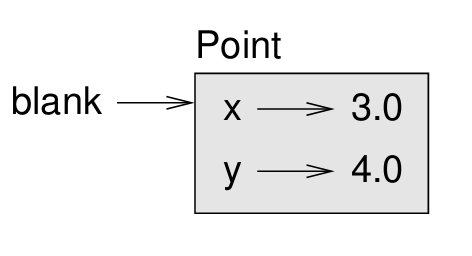
\includegraphics[width=0.7\linewidth]{images/chapter_15_1.png} % Ajusta el nombre del archivo
\caption{Diagrama de objeto.}
\label{fig:diagrama_estado}
\end{figure}

La cabecera indica que la nueva clase se llama \texttt{Point}. El cuerpo es un docstring que explica para qué sirve la clase. Puedes definir variables y métodos dentro de una definición de clase, pero volveremos a eso más adelante.

Definir una clase llamada \texttt{Point} crea un objeto de clase.

\begin{lstlisting}[language=Python]
>>> Point
<class '__main__.Point'>
\end{lstlisting}

Como \texttt{Point} se define en el nivel superior, su ``nombre completo'' es \texttt{\_\_main\_\_.Point}.

El objeto de clase es como una fábrica para crear objetos. Para crear un \texttt{Point}, llamas a \texttt{Point} como si fuera una función.

\begin{lstlisting}[language=Python]
>>> blank = Point()
>>> blank
<__main__.Point object at 0xb7e9d3ac>
\end{lstlisting}

El valor de retorno es una referencia a un objeto \texttt{Point}, que asignamos a \texttt{blank}.

Crear un nuevo objeto se llama \textbf{instanciación}, y el objeto es una \textbf{instancia} de la clase.

Cuando imprimes una instancia, Python te dice a qué clase pertenece y dónde está almacenada en memoria (el prefijo \texttt{0x} significa que el siguiente número está en hexadecimal).

Cada objeto es una instancia de alguna clase, por lo que ``objeto'' e ``instancia'' son intercambiables. Pero en este capítulo usaré ``instancia'' para indicar que estoy hablando de un tipo definido por el programador.

\section{Atributos}

Puedes asignar valores a una instancia usando notación de punto:

\begin{lstlisting}[language=Python]
>>> blank.x = 3.0
>>> blank.y = 4.0
\end{lstlisting}

Esta sintaxis es similar a la sintaxis para seleccionar una variable de un módulo, como \texttt{math.pi} o \texttt{string.whitespace}. En este caso, sin embargo, estamos asignando valores a elementos nombrados de un objeto. Estos elementos se llaman \textbf{atributos}.

Como sustantivo, ``atributo'' se pronuncia con énfasis en la primera sílaba, a diferencia de ``atribuir'', que es un verbo.

La Figura 15.1 es un diagrama de estado que muestra el resultado de estas asignaciones. Un diagrama de estado que muestra un objeto y sus atributos se llama \textbf{diagrama de objetos}.

La variable \texttt{blank} se refiere a un objeto \texttt{Point}, que contiene dos atributos. Cada atributo se refiere a un número de punto flotante.

Puedes leer el valor de un atributo usando la misma sintaxis:

\begin{lstlisting}[language=Python]
>>> blank.y
4.0
>>> x = blank.x
>>> x
3.0
\end{lstlisting}

La expresión \texttt{blank.x} significa: ``Ve al objeto al que \texttt{blank} se refiere y obtén el valor de \texttt{x}''. En el ejemplo, asignamos ese valor a una variable llamada \texttt{x}. No hay conflicto entre la variable \texttt{x} y el atributo \texttt{x}.

Puedes usar notación de punto como parte de cualquier expresión. Por ejemplo:

\begin{lstlisting}[language=Python]
>>> '(%g, %g)' % (blank.x, blank.y)
'(3.0, 4.0)'
>>> distance = math.sqrt(blank.x**2 + blank.y**2)
>>> distance
5.0
\end{lstlisting}

Puedes pasar una instancia como argumento de la manera habitual. Por ejemplo:

\begin{lstlisting}[language=Python]
def print_point(p):
    print('(%g, %g)' % (p.x, p.y))
\end{lstlisting}

\texttt{print\_point} toma un punto como argumento y lo muestra en notación matemática. Para invocarlo, puedes pasar \texttt{blank} como argumento:

\begin{lstlisting}[language=Python]
>>> print_point(blank)
(3.0, 4.0)
\end{lstlisting}

Dentro de la función, \texttt{p} es un alias para \texttt{blank}, por lo que si la función modifica \texttt{p}, \texttt{blank} cambia.

Como ejercicio, escribe una función llamada \texttt{distance\_between\_points} que tome dos \texttt{Points} como argumentos y devuelva la distancia entre ellos.

\section{Rectángulos}

A veces es obvio cuáles deberían ser los atributos de un objeto, pero otras veces tienes que tomar decisiones. Por ejemplo, imagina que estás diseñando una clase para representar rectángulos. ¿Qué atributos usarías para especificar la ubicación y el tamaño del rectángulo? Puedes ignorar el ángulo; para simplificar, asume que el rectángulo es vertical u horizontal.

Hay al menos dos posibilidades:

\begin{itemize}
    \item Podrías especificar una esquina del rectángulo (o el centro), el ancho y la altura.
    \item Podrías especificar dos esquinas opuestas.
\end{itemize}

En este punto es difícil decir si una es mejor que la otra, así que implementaremos la primera, solo como ejemplo.

Aquí está la definición de la clase:

\begin{figure}[h]
\centering
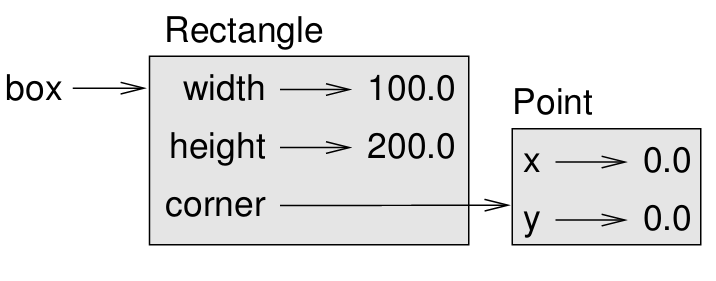
\includegraphics[width=0.7\linewidth]{images/chapter_15_2.png} % Ajusta el nombre del archivo
\caption{Diagrama de objeto.}
\label{fig:diagrama_estado}
\end{figure}

\begin{lstlisting}[language=Python]
class Rectangle:
    """Representa un rectángulo.
    
    atributos: width, height, corner.
    """
\end{lstlisting}

El docstring enumera los atributos: \texttt{width} y \texttt{height} son números; \texttt{corner} es un objeto \texttt{Point} que especifica la esquina inferior izquierda.

Para representar un rectángulo, debes instanciar un objeto \texttt{Rectangle} y asignar valores a los atributos:

\begin{lstlisting}[language=Python]
box = Rectangle()
box.width = 100.0
box.height = 200.0
box.corner = Point()
box.corner.x = 0.0
box.corner.y = 0.0
\end{lstlisting}

La expresión \texttt{box.corner.x} significa: ``Ve al objeto al que \texttt{box} se refiere y selecciona el atributo llamado \texttt{corner}; luego ve a ese objeto y selecciona el atributo llamado \texttt{x}''.

La Figura 15.2 muestra el estado de este objeto. Un objeto que es un atributo de otro objeto está \textbf{incrustado}.

\section{Instancias como valores de retorno}

Las funciones pueden devolver instancias. Por ejemplo, \texttt{find\_center} toma un \texttt{Rectangle} como argumento y devuelve un \texttt{Point} que contiene las coordenadas del centro del \texttt{Rectangle}:

\begin{lstlisting}[language=Python]
def find_center(rect):
    p = Point()
    p.x = rect.corner.x + rect.width/2
    p.y = rect.corner.y + rect.height/2
    return p
\end{lstlisting}

Aquí hay un ejemplo que pasa \texttt{box} como argumento y asigna el \texttt{Point} resultante a \texttt{center}:

\begin{lstlisting}[language=Python]
>>> center = find_center(box)
>>> print_point(center)
(50, 100)
\end{lstlisting}

\section{Los objetos son mutables}

Puedes cambiar el estado de un objeto haciendo una asignación a uno de sus atributos. Por ejemplo, para cambiar el tamaño de un rectángulo sin cambiar su posición, puedes modificar los valores de \texttt{width} y \texttt{height}:

\begin{lstlisting}[language=Python]
box.width = box.width + 50
box.height = box.height + 100
\end{lstlisting}

También puedes escribir funciones que modifiquen objetos. Por ejemplo, \texttt{grow\_rectangle} toma un objeto \texttt{Rectangle} y dos números, \texttt{dwidth} y \texttt{dheight}, y suma los números al ancho y altura del rectángulo:

\begin{lstlisting}[language=Python]
def grow_rectangle(rect, dwidth, dheight):
    rect.width += dwidth
    rect.height += dheight
\end{lstlisting}

Aquí hay un ejemplo que demuestra el efecto:

\begin{lstlisting}[language=Python]
>>> box.width, box.height
(150.0, 300.0)
>>> grow_rectangle(box, 50, 100)
>>> box.width, box.height
(200.0, 400.0)
\end{lstlisting}

Dentro de la función, \texttt{rect} es un alias para \texttt{box}, por lo que cuando la función modifica \texttt{rect}, \texttt{box} cambia.

Como ejercicio, escribe una función llamada \texttt{move\_rectangle} que tome un \texttt{Rectangle} y dos números llamados \texttt{dx} y \texttt{dy}. Debe cambiar la ubicación del rectángulo sumando \texttt{dx} a la coordenada \texttt{x} de \texttt{corner} y sumando \texttt{dy} a la coordenada \texttt{y} de \texttt{corner}.

\section{Copiado}

El uso de alias puede hacer que un programa sea difícil de leer porque los cambios en un lugar pueden tener efectos inesperados en otro lugar. Es difícil hacer un seguimiento de todas las variables que podrían referirse a un objeto dado.

Copiar un objeto es a menudo una alternativa al uso de alias. El módulo \texttt{copy} contiene una función llamada \texttt{copy} que puede duplicar cualquier objeto:

\begin{lstlisting}[language=Python]
>>> p1 = Point()
>>> p1.x = 3.0
>>> p1.y = 4.0

>>> import copy
>>> p2 = copy.copy(p1)
\end{lstlisting}

\texttt{p1} y \texttt{p2} contienen los mismos datos, pero no son el mismo \texttt{Point}.

\begin{lstlisting}[language=Python]
>>> print_point(p1)
(3, 4)
>>> print_point(p2)
(3, 4)
>>> p1 is p2
False
>>> p1 == p2
False
\end{lstlisting}

\begin{figure}[h]
\centering
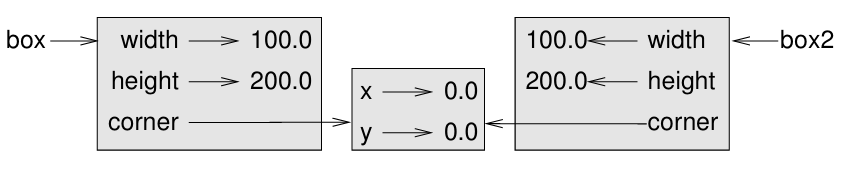
\includegraphics[width=0.7\linewidth]{images/chapter_15_3.png} % Ajusta el nombre del archivo
\caption{Diagrama de onjeto.}
\label{fig:diagrama_estado}
\end{figure}

\begin{lstlisting}
>>> p1 == p2
False
\end{lstlisting}
El operador \texttt{is} indica que \texttt{p1} y \texttt{p2} no son el mismo objeto, que es lo que esperábamos. Pero podrías haber esperado que \texttt{==} devolviera \texttt{True} porque estos puntos contienen los mismos datos. En ese caso, te decepcionará saber que para instancias, el comportamiento predeterminado del operador \texttt{==} es el mismo que el operador \texttt{is}; verifica la identidad del objeto, no la equivalencia del objeto. Esto se debe a que, para tipos definidos por el programador, Python no sabe qué debería considerarse equivalente. Al menos, no todavía.

Si usas \texttt{copy.copy} para duplicar un \texttt{Rectangle}, encontrarás que copia el objeto \texttt{Rectangle} pero no el \texttt{Point} incrustado.

\begin{lstlisting}[language=Python]
>>> box2 = copy.copy(box)
>>> box2 is box
False
>>> box2.corner is box.corner
True
\end{lstlisting}

La Figura 15.3 muestra cómo se ve el diagrama de objetos. Esta operación se llama \textbf{copia superficial} porque copia el objeto y cualquier referencia que contenga, pero no los objetos incrustados.

Para la mayoría de las aplicaciones, esto no es lo que deseas. En este ejemplo, invocar \texttt{grow\_rectangle} en uno de los \texttt{Rectangles} no afectaría al otro, pero invocar \texttt{move\_rectangle} en cualquiera de ellos afectaría a ambos. Este comportamiento es confuso y propenso a errores.

Afortunadamente, el módulo \texttt{copy} proporciona un método llamado \texttt{deepcopy} que copia no solo el objeto sino también los objetos a los que se refiere, y los objetos a los que ellos se refieren, y así sucesivamente. No te sorprenderá saber que esta operación se llama \textbf{copia profunda}.

\begin{lstlisting}[language=Python]
>>> box3 = copy.deepcopy(box)
>>> box3 is box
False
>>> box3.corner is box.corner
False
\end{lstlisting}

\texttt{box3} y \texttt{box} son objetos completamente separados.

Como ejercicio, escribe una versión de \texttt{move\_rectangle} que cree y devuelva un nuevo \texttt{Rectangle} en lugar de modificar el antiguo.

\section{Depuración}

Cuando comienzas a trabajar con objetos, es probable que encuentres algunas excepciones nuevas. Si intentas acceder a un atributo que no existe, obtienes un \texttt{AttributeError}:

\begin{lstlisting}[language=Python]
>>> p = Point()
>>> p.x = 3
>>> p.y = 4
>>> p.z
AttributeError: Point instance has no attribute 'z'
\end{lstlisting}

Si no estás seguro de qué tipo es un objeto, puedes preguntar:

\begin{lstlisting}[language=Python]
>>> type(p)
<class '__main__.Point'>
\end{lstlisting}

También puedes usar \texttt{isinstance} para verificar si un objeto es una instancia de una clase:

\begin{lstlisting}[language=Python]
>>> isinstance(p, Point)
True
\end{lstlisting}

Si no estás seguro de si un objeto tiene un atributo particular, puedes usar la función incorporada \texttt{hasattr}:

\begin{lstlisting}[language=Python]
>>> hasattr(p, 'x')
True
>>> hasattr(p, 'z')
False
\end{lstlisting}

El primer argumento puede ser cualquier objeto; el segundo argumento es una cadena que contiene el nombre del atributo.

También puedes usar una sentencia \texttt{try} para ver si el objeto tiene los atributos que necesitas:

\begin{lstlisting}[language=Python]
try:
    x = p.x
except AttributeError:
    x = 0
\end{lstlisting}

Este enfoque puede facilitar la escritura de funciones que trabajan con diferentes tipos; más sobre ese tema en la Sección 17.9.

\section{Glosario}

\begin{description}
    \item[clase:] Un tipo definido por el programador. Una definición de clase crea un nuevo objeto de clase.
    \item[objeto de clase:] Un objeto que contiene información sobre un tipo definido por el programador. El objeto de clase se puede usar para crear instancias del tipo.
    \item[instancia:] Un objeto que pertenece a una clase.
    \item[instanciar:] Crear un nuevo objeto.
    \item[atributo:] Uno de los valores nombrados asociados con un objeto.
    \item[objeto incrustado:] Un objeto que se almacena como atributo de otro objeto.
    \item[copia superficial:] Copiar el contenido de un objeto, incluidas las referencias a objetos incrustados; implementado por la función \texttt{copy} en el módulo \texttt{copy}.
    \item[copia profunda:] Copiar el contenido de un objeto así como cualquier objeto incrustado, y cualquier objeto incrustado en ellos, y así sucesivamente; implementado por la función \texttt{deepcopy} en el módulo \texttt{copy}.
    \item[diagrama de objetos:] Un diagrama que muestra objetos, sus atributos y los valores de los atributos.
\end{description}

\section{Ejercicios}

\textbf{Ejercicio 15.1.} Escribe una definición para una clase llamada \texttt{Circle} con atributos \texttt{center} y \texttt{radius}, donde \texttt{center} es un objeto \texttt{Point} y \texttt{radius} es un número.

Instancia un objeto \texttt{Circle} que represente un círculo con su centro en $(150,100)$ y radio 75.

Escribe una función llamada \texttt{point\_in\_circle} que tome un \texttt{Circle} y un \texttt{Point} y devuelva \texttt{True} si el \texttt{Point} está dentro o en el límite del círculo.

Escribe una función llamada \texttt{rect\_in\_circle} que tome un \texttt{Circle} y un \texttt{Rectangle} y devuelva \texttt{True} si el \texttt{Rectangle} está completamente dentro o en el límite del círculo.

Escribe una función llamada \texttt{rect\_circle\_overlap} que tome un \texttt{Circle} y un \texttt{Rectangle} y devuelva \texttt{True} si alguna de las esquinas del \texttt{Rectangle} cae dentro del círculo. O como una versión más desafiante, devuelve \texttt{True} si cualquier parte del \texttt{Rectangle} cae dentro del círculo.

Solución: \url{https://thinkpython.com/code/Circle.py}.

\textbf{Ejercicio 15.2.} Escribe una función llamada \texttt{draw\_rect} que tome un objeto \texttt{Turtle} y un \texttt{Rectangle} y use la \texttt{Turtle} para dibujar el \texttt{Rectangle}. Consulta el Capítulo 4 para ver ejemplos de uso de objetos \texttt{Turtle}.

Escribe una función llamada \texttt{draw\_circle} que tome una \texttt{Turtle} y un \texttt{Circle} y dibuje el \texttt{Circle}.

Solución: \url{https://thinkpython.com/code/draw.py}.
%chapter 16

\chapter{Clases y funciones}

Ahora que sabemos cómo crear nuevos tipos, el siguiente paso es escribir funciones que tomen objetos definidos por el programador como parámetros y los devuelvan como resultados. En este capítulo también presento el "estilo de programación funcional" y dos nuevos planes de desarrollo de programas.

Los ejemplos de código de este capítulo están disponibles en \url{https://thinkpython.com/code/Time1.py}. Las soluciones a los ejercicios se encuentran en \url{https://thinkpython.com/code/Time1_soln.py}.

\section{Tiempo}

Como otro ejemplo de un tipo definido por el programador, definiremos una clase llamada \texttt{Time} que registra la hora del día. La definición de la clase se ve así:

\begin{lstlisting}[language=Python]
class Time:
    """Representa la hora del día.
    atributos: hour, minute, second
    """
\end{lstlisting}

Podemos crear un nuevo objeto \texttt{Time} y asignar atributos para horas, minutos y segundos:

\begin{lstlisting}[language=Python]
time = Time()
time.hour = 11
time.minute = 59
time.second = 30
\end{lstlisting}

El diagrama de estado para el objeto \texttt{Time} se muestra en la Figura 16.1.

Como ejercicio, escribe una función llamada \texttt{print\_time} que tome un objeto \texttt{Time} y lo imprima en el formato \texttt{hour:minute:second}. Pista: la secuencia de formato \texttt{'\%02d'} imprime un entero usando al menos dos dígitos, incluyendo un cero inicial si es necesario.

Escribe una función booleana llamada \texttt{is\_after} que tome dos objetos \texttt{Time}, \texttt{t1} y \texttt{t2}, y devuelva \texttt{True} si \texttt{t1} sigue cronológicamente a \texttt{t2} y \texttt{False} en caso contrario. Desafío: no uses una sentencia \texttt{if}.

\begin{figure}[h]
\centering
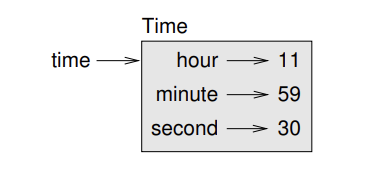
\includegraphics[width=0.5\textwidth]{./images/chapter_16_1.png}
\caption{Diagrama de objeto.}
\label{fig:time_diagram}
\end{figure}

\section{Funciones puras}

En las próximas secciones, escribiremos dos funciones que suman valores de tiempo. Estas demuestran dos tipos de funciones: funciones puras y modificadores. También demuestran un plan de desarrollo que llamaré "prototipo y parche", que es una forma de abordar un problema complejo comenzando con un prototipo simple y tratando las complicaciones de manera incremental.

Aquí hay un prototipo simple de \texttt{add\_time}:

\begin{lstlisting}[language=Python]
def add_time(t1, t2):
    sum = Time()
    sum.hour = t1.hour + t2.hour
    sum.minute = t1.minute + t2.minute
    sum.second = t1.second + t2.second
    return sum
\end{lstlisting}

La función crea un nuevo objeto \texttt{Time}, inicializa sus atributos y devuelve una referencia al nuevo objeto. Esto se llama una \textbf{función pura} porque no modifica ninguno de los objetos que se le pasan como argumentos y no tiene ningún efecto, como mostrar un valor u obtener entrada del usuario, aparte de devolver un valor.

Para probar esta función, crearé dos objetos \texttt{Time}: \texttt{start} contiene la hora de inicio de una película, como \textit{Monty Python and the Holy Grail}, y \texttt{duration} contiene la duración de la película, que es de una hora y 35 minutos.

\texttt{add\_time} calcula cuándo terminará la película.

\begin{lstlisting}[language=Python]
>>> start = Time()
>>> start.hour = 9
>>> start.minute = 45
>>> start.second = 0
>>> duration = Time()
>>> duration.hour = 1
>>> duration.minute = 35
>>> duration.second = 0
>>> done = add_time(start, duration)
>>> print_time(done)
10:80:00
\end{lstlisting}

El resultado, \texttt{10:80:00}, podría no ser lo que esperabas. El problema es que esta función no maneja los casos donde el número de segundos o minutos suma más de sesenta. Cuando eso sucede, tenemos que "llevar" los segundos extra a la columna de minutos o los minutos extra a la columna de horas.

Aquí hay una versión mejorada:

\begin{lstlisting}[language=Python]
def add_time(t1, t2):
    sum = Time()
    sum.hour = t1.hour + t2.hour
    sum.minute = t1.minute + t2.minute
    sum.second = t1.second + t2.second

    if sum.second >= 60:
        sum.second -= 60
        sum.minute += 1

    if sum.minute >= 60:
        sum.minute -= 60
        sum.hour += 1

    return sum
\end{lstlisting}

Aunque esta función es correcta, está empezando a crecer. Veremos una alternativa más corta más adelante.

\section{Modificadores}

A veces es útil que una función modifique los objetos que recibe como parámetros. En ese caso, los cambios son visibles para quien llama. Las funciones que funcionan así se llaman \textbf{modificadores}.

\texttt{increment}, que agrega una cantidad dada de segundos a un objeto \texttt{Time}, puede escribirse naturalmente como un modificador. Aquí hay un borrador:

\begin{lstlisting}[language=Python]
def increment(time, seconds):
    time.second += seconds

    if time.second >= 60:
        time.second -= 60
        time.minute += 1

    if time.minute >= 60:
        time.minute -= 60
        time.hour += 1
\end{lstlisting}

La primera línea realiza la operación básica; el resto maneja los casos especiales que vimos antes.

¿Es esta función correcta? ¿Qué pasa si \texttt{seconds} es mucho mayor que sesenta?

En ese caso, no es suficiente con llevar una vez; tenemos que seguir haciéndolo hasta que \texttt{time.second} sea menor que sesenta. Una solución es reemplazar las sentencias \texttt{if} con sentencias \texttt{while}. Eso haría que la función fuera correcta, pero no muy eficiente. Como ejercicio, escribe una versión correcta de \texttt{increment} que no contenga bucles.

Cualquier cosa que se pueda hacer con modificadores también se puede hacer con funciones puras. De hecho, algunos lenguajes de programación solo permiten funciones puras. Hay evidencia de que los programas que usan funciones puras se desarrollan más rápido y son menos propensos a errores que los programas que usan modificadores. Pero los modificadores son convenientes a veces, y los programas funcionales tienden a ser menos eficientes.

En general, recomiendo que escribas funciones puras siempre que sea razonable y recurras a modificadores solo si hay una ventaja convincente. Este enfoque podría llamarse \textbf{estilo de programación funcional}.

Como ejercicio, escribe una versión "pura" de \texttt{increment} que cree y devuelva un nuevo objeto \texttt{Time} en lugar de modificar el parámetro.

\section{Prototipado versus planificación}

El plan de desarrollo que estoy demostrando se llama "prototipo y parche". Para cada función, escribí un prototipo que realizaba el cálculo básico y luego lo probé, corrigiendo errores en el camino.

Este enfoque puede ser efectivo, especialmente si aún no tienes una comprensión profunda del problema. Pero las correcciones incrementales pueden generar código innecesariamente complicado (ya que maneja muchos casos especiales) y poco confiable (ya que es difícil saber si has encontrado todos los errores).

Una alternativa es el \textbf{desarrollo diseñado}, en el que una comprensión de alto nivel del problema puede hacer que la programación sea mucho más fácil. En este caso, la idea es que un objeto \texttt{Time} es en realidad un número de tres dígitos en base 60. El atributo \texttt{second} es la "columna de las unidades", el atributo \texttt{minute} es la "columna de los sesentas" y el atributo \texttt{hour} es la "columna de los tres mil seiscientos".

Cuando escribimos \texttt{add\_time} e \texttt{increment}, estábamos haciendo efectivamente una suma en base 60, razón por la cual teníamos que llevar de una columna a la siguiente.

Esta observación sugiere otro enfoque para todo el problema: podemos convertir objetos \texttt{Time} a enteros y aprovechar el hecho de que la computadora sabe cómo hacer aritmética con enteros.

Aquí hay una función que convierte \texttt{Time} a enteros:

\begin{lstlisting}[language=Python]
def time_to_int(time):
    minutes = time.hour * 60 + time.minute
    seconds = minutes * 60 + time.second
    return seconds
\end{lstlisting}

Y aquí hay una función que convierte un entero a \texttt{Time} (recuerda que \texttt{divmod} divide el primer argumento por el segundo y devuelve el cociente y el resto como una tupla):

\begin{lstlisting}[language=Python]
def int_to_time(seconds):
    time = Time()
    minutes, time.second = divmod(seconds, 60)
    time.hour, time.minute = divmod(minutes, 60)
    return time
\end{lstlisting}

Podrías tener que pensar un poco y ejecutar algunas pruebas para convencerte de que estas funciones son correctas. Una forma de probarlas es verificar que \texttt{time\_to\_int(int\_to\_time(x)) == x} para muchos valores de \texttt{x}. Este es un ejemplo de una verificación de consistencia.

Una vez que estés convencido de que son correctas, puedes usarlas para reescribir \texttt{add\_time}:

\begin{lstlisting}[language=Python]
def add_time(t1, t2):
    seconds = time_to_int(t1) + time_to_int(t2)
    return int_to_time(seconds)
\end{lstlisting}

Esta versión es más corta que la original y más fácil de verificar. Como ejercicio, reescribe \texttt{increment} usando \texttt{time\_to\_int} e \texttt{int\_to\_time}.

En algunos aspectos, convertir de base 60 a base 10 y viceversa es más difícil que simplemente lidiar con valores de tiempo. La conversión de base es más abstracta; nuestra intuición para manejar valores de tiempo es mejor.

Pero si tenemos la idea de tratar los tiempos como números en base 60 y hacemos el esfuerzo de escribir las funciones de conversión (\texttt{time\_to\_int} e \texttt{int\_to\_time}), obtenemos un programa que es más corto, más fácil de leer y depurar, y más confiable.

También es más fácil agregar características más adelante. Por ejemplo, imagina restar dos \texttt{Time} para encontrar la duración entre ellos. El enfoque ingenuo sería implementar la resta con préstamo. Usar las funciones de conversión sería más fácil y más probable que sea correcto.

Irónicamente, a veces hacer un problema más difícil (o más general) lo hace más fácil (porque hay menos casos especiales y menos oportunidades de error).

\section{Depuración}

Un objeto \texttt{Time} está bien formado si los valores de \texttt{minute} y \texttt{second} están entre 0 y 60 (incluyendo 0 pero no 60) y si \texttt{hour} es positivo. \texttt{hour} y \texttt{minute} deben ser valores enteros, pero podríamos permitir que \texttt{second} tenga una parte fraccionaria.

Requisitos como estos se llaman \textbf{invariantes} porque siempre deben ser verdaderos. Dicho de otra manera, si no son verdaderos, algo ha salido mal.

Escribir código para verificar invariantes puede ayudar a detectar errores y encontrar sus causas. Por ejemplo, podrías tener una función como \texttt{valid\_time} que toma un objeto \texttt{Time} y devuelve \texttt{False} si viola un invariante:

\begin{lstlisting}[language=Python]
def valid_time(time):
    if time.hour < 0 or time.minute < 0 or time.second < 0:
        return False
    if time.minute >= 60 or time.second >= 60:
        return False
    return True
\end{lstlisting}

Al comienzo de cada función, podrías verificar los argumentos para asegurarte de que son válidos:

\begin{lstlisting}[language=Python]
def add_time(t1, t2):
    if not valid_time(t1) or not valid_time(t2):
        raise ValueError('invalid Time object in add_time')
    seconds = time_to_int(t1) + time_to_int(t2)
    return int_to_time(seconds)
\end{lstlisting}

O podrías usar una \textbf{sentencia assert}, que verifica un invariante dado y genera una excepción si falla:

\begin{lstlisting}[language=Python]
def add_time(t1, t2):
    assert valid_time(t1) and valid_time(t2)
    seconds = time_to_int(t1) + time_to_int(t2)
    return int_to_time(seconds)
\end{lstlisting}

Las sentencias \texttt{assert} son útiles porque distinguen el código que maneja condiciones normales del código que verifica errores.

\section{Glosario}

\begin{description}
\item[prototipo y parche:] Un plan de desarrollo que implica escribir un borrador de un programa, probarlo y corregir errores a medida que se encuentran.
\item[desarrollo diseñado:] Un plan de desarrollo que implica una comprensión de alto nivel del problema y más planificación que el desarrollo incremental o el desarrollo de prototipos.
\item[función pura:] Una función que no modifica ninguno de los objetos que recibe como argumentos. La mayoría de las funciones puras son fructíferas.
\item[modificador:] Una función que cambia uno o más de los objetos que recibe como argumentos. La mayoría de los modificadores son nulos; es decir, devuelven \texttt{None}.
\item[estilo de programación funcional:] Un estilo de diseño de programas en el que la mayoría de las funciones son puras.
\item[invariante:] Una condición que siempre debe ser verdadera durante la ejecución de un programa.
\item[sentencia assert:] Una sentencia que verifica una condición y genera una excepción si falla.
\end{description}

\section{Ejercicios}

Los ejemplos de código de este capítulo están disponibles en \url{https://thinkpython.com/code/Time1.py}; las soluciones a los ejercicios están disponibles en \url{https://thinkpython.com/code/Time1_soln.py}.

\begin{enumerate}
\item \textbf{Ejercicio 16.1.} Escribe una función llamada \texttt{mul\_time} que tome un objeto \texttt{Time} y un número y devuelva un nuevo objeto \texttt{Time} que contenga el producto del \texttt{Time} original y el número.

Luego usa \texttt{mul\_time} para escribir una función que tome un objeto \texttt{Time} que represente el tiempo de finalización en una carrera y un número que represente la distancia, y devuelva un objeto \texttt{Time} que represente el ritmo promedio (tiempo por milla).

\item \textbf{Ejercicio 16.2.} El módulo \texttt{datetime} proporciona objetos de tiempo similares a los objetos \texttt{Time} de este capítulo, pero ofrecen un conjunto rico de métodos y operadores. Lee la documentación en \url{http://docs.python.org/3/library/datetime.html}.

\begin{enumerate}
\item Usa el módulo \texttt{datetime} para escribir un programa que obtenga la fecha actual e imprima el día de la semana.
\item Escribe un programa que tome un cumpleaños como entrada e imprima la edad del usuario y el número de días, horas, minutos y segundos hasta su próximo cumpleaños.
\item Para dos personas nacidas en días diferentes, hay un día en el que uno es el doble de viejo que el otro. Ese es su "Día Doble". Escribe un programa que tome dos fechas de nacimiento y calcule su Día Doble.
\item Para un poco más de desafío, escribe la versión más general que calcule el día en el que una persona es $n$ veces mayor que la otra.
\end{enumerate}

Solución: \url{https://thinkpython.com/code/double.py}
\end{enumerate}
\chapter{Clases y métodos}

Aunque hemos estado usando algunas características orientadas a objetos de Python, los programas de los últimos dos capítulos no son realmente orientados a objetos porque no representan las relaciones entre tipos definidos por el programador y las funciones que operan sobre ellos. El siguiente paso es transformar esas funciones en métodos que hagan explícitas estas relaciones.

Los ejemplos de código de este capítulo están disponibles en \url{https://thinkpython.com/code/Time2.py}, y las soluciones a los ejercicios están en \url{https://thinkpython.com/code/Point2_soln.py}.

\section{Características orientadas a objetos}

Python es un \textbf{lenguaje de programación orientado a objetos}, lo que significa que proporciona características que soportan programación orientada a objetos, que tiene estas características definitorias:

\begin{itemize}
\item Los programas incluyen definiciones de clases y métodos.
\item La mayor parte del cálculo se expresa en términos de operaciones sobre objetos.
\item Los objetos a menudo representan cosas del mundo real, y los métodos a menudo corresponden a formas en que las cosas del mundo real interactúan.
\end{itemize}

Por ejemplo, la clase Time definida en el Capítulo 16 corresponde a cómo las personas registran la hora del día, y las funciones que definimos corresponden a las cosas que la gente hace con las horas. De manera similar, las clases Point y Rectangle del Capítulo 15 corresponden a los conceptos matemáticos de punto y rectángulo.

Hasta ahora, no hemos aprovechado las características que Python proporciona para soportar programación orientada a objetos. Estas características no son estrictamente necesarias; la mayoría proporciona sintaxis alternativa para cosas que ya hemos hecho. Pero en muchos casos, la alternativa es más concisa y transmite con mayor precisión la estructura del programa.

Por ejemplo, en Time1.py no hay una conexión obvia entre la definición de clase y las definiciones de funciones que siguen. Tras examinarlo, es aparente que cada función toma al menos un objeto Time como argumento.

\section{Impresión de objetos}

En el Capítulo 16, definimos una clase llamada Time y en la Sección 16.1, escribiste una función llamada print\_time:

\begin{lstlisting}[language=Python]
class Time:
    """Representa la hora del día."""
    
def print_time(time):
    print('%.2d:%.2d:%.2d' % (time.hour, time.minute, time.second))
\end{lstlisting}

Para llamar a esta función, debes pasar un objeto Time como argumento:

\begin{lstlisting}[language=Python]
>>> start = Time()
>>> start.hour = 9
>>> start.minute = 45
>>> start.second = 00
>>> print_time(start)
09:45:00
\end{lstlisting}

Para hacer de print\_time un método, todo lo que tenemos que hacer es mover la definición de la función dentro de la definición de la clase. Observa el cambio en la indentación.

\begin{lstlisting}[language=Python]
class Time:
    def print_time(time):
        print('%.2d:%.2d:%.2d' % (time.hour, time.minute, time.second))
\end{lstlisting}

Ahora hay dos formas de llamar a print\_time. La primera (y menos común) es usar sintaxis de función:

\begin{lstlisting}[language=Python]
>>> Time.print_time(start)
09:45:00
\end{lstlisting}

En este uso de la notación de punto, Time es el nombre de la clase, y print\_time es el nombre del método. start se pasa como parámetro.

La segunda (y más concisa) es usar sintaxis de método:

\begin{lstlisting}[language=Python]
>>> start.print_time()
09:45:00
\end{lstlisting}

\section{Otro ejemplo}

En este uso de la notación de punto, print\_time es el nombre del método (nuevamente), y start es el objeto sobre el que se invoca el método, llamado sujeto. Así como el sujeto de una oración es de lo que trata la oración, el sujeto de una invocación de método es de lo que trata el método.

Dentro del método, el sujeto se asigna al primer parámetro, por lo que en este caso start se asigna a time.

Por convención, el primer parámetro de un método se llama self, por lo que sería más común escribir print\_time así:

\begin{lstlisting}[language=Python]
class Time:
    def print_time(self):
        print('%.2d:%.2d:%.2d' % (self.hour, self.minute, self.second))
\end{lstlisting}

La razón de esta convención es una metáfora implícita:

\begin{itemize}
\item La sintaxis para una llamada a función, print\_time(start), sugiere que la función es el agente activo. Dice algo como: "¡Oye print\_time! Aquí hay un objeto para que imprimas."
\item En programación orientada a objetos, los objetos son los agentes activos. Una invocación de método como start.print\_time() dice "¡Oye start! Por favor imprímete."
\end{itemize}

Este cambio de perspectiva podría ser más educado, pero no es obvio que sea útil. En los ejemplos que hemos visto hasta ahora, puede que no lo sea. Pero a veces transferir la responsabilidad de las funciones a los objetos permite escribir funciones (o métodos) más versátiles y facilita el mantenimiento y reutilización del código.

Como ejercicio, reescribe time\_to\_int (de la Sección 16.4) como un método. Podrías sentirte tentado a reescribir int\_to\_time como un método también, pero eso no tendría mucho sentido porque no habría ningún objeto sobre el que invocarlo.

\section{Un ejemplo más complicado}

Aquí hay una versión de increment (de la Sección 16.3) reescrita como método:

\begin{lstlisting}[language=Python]
# dentro de la clase Time:
def increment(self, seconds):
    seconds += self.time_to_int()
    return int_to_time(seconds)
\end{lstlisting}

Esta versión asume que time\_to\_int está escrito como método. Además, nota que es una función pura, no un modificador.

Aquí está cómo invocarías increment:

\begin{lstlisting}[language=Python]
>>> start.print_time()
09:45:00
>>> end = start.increment(1337)
>>> end.print_time()
10:07:17
\end{lstlisting}

El sujeto, start, se asigna al primer parámetro, self. El argumento, 1337, se asigna al segundo parámetro, seconds.

Este mecanismo puede ser confuso, especialmente si cometes un error. Por ejemplo, si invocas increment con dos argumentos, obtienes:

\begin{lstlisting}[language=Python]
>>> end = start.increment(1337, 460)
TypeError: increment() takes 2 positional arguments but 3 were given
\end{lstlisting}

El mensaje de error es inicialmente confuso, porque solo hay dos argumentos entre paréntesis. Pero el sujeto también se considera un argumento, así que en total son tres.

Por cierto, un argumento posicional es un argumento que no tiene un nombre de parámetro; es decir, no es un argumento de palabra clave. En esta llamada a función:

\begin{lstlisting}[language=Python]
sketch(parrot, cage, dead=True)
\end{lstlisting}

parrot y cage son posicionales, y dead es un argumento de palabra clave.

\section{El método init}

El método \_\_init\_\_ (abreviatura de "inicialización") es un método especial que se invoca cuando se instancia un objeto. Su nombre completo es \_\_init\_\_ (dos caracteres de subrayado, seguidos de init, y luego dos más). Un método \_\_init\_\_ para la clase Time podría verse así:

\begin{lstlisting}[language=Python]
# dentro de la clase Time:
def __init__(self, hour=0, minute=0, second=0):
    self.hour = hour
    self.minute = minute
    self.second = second
\end{lstlisting}

Es común que los parámetros de \_\_init\_\_ tengan los mismos nombres que los atributos. La declaración:

\begin{lstlisting}[language=Python]
self.hour = hour
\end{lstlisting}

almacena el valor del parámetro hour como un atributo de self.

Los parámetros son opcionales, así que si llamas a Time sin argumentos, obtienes los valores predeterminados.

\begin{lstlisting}[language=Python]
>>> time = Time()
>>> time.print_time()
00:00:00
\end{lstlisting}

Si proporcionas un argumento, anula hour:

\begin{lstlisting}[language=Python]
>>> time = Time(9)
>>> time.print_time()
09:00:00
\end{lstlisting}

Si proporcionas dos argumentos, anulan hour y minute:

\begin{lstlisting}[language=Python]
>>> time = Time(9, 45)
>>> time.print_time()
09:45:00
\end{lstlisting}

Y si proporcionas tres argumentos, anulan los tres valores predeterminados.

Como ejercicio, escribe un método \_\_init\_\_ para la clase Point que tome x e y como parámetros opcionales y los asigne a los atributos correspondientes.

\section{El método \_\_str\_\_}

\_\_str\_\_ es un método especial, como \_\_init\_\_, que se supone debe devolver una representación en cadena de un objeto.

Por ejemplo, aquí hay un método str para objetos Time:

\begin{lstlisting}[language=Python]
# dentro de la clase Time:
def __str__(self):
    return '%.2d:%.2d:%.2d' % (self.hour, self.minute, self.second)
\end{lstlisting}

Cuando imprimes un objeto, Python invoca el método str:

\begin{lstlisting}[language=Python]
>>> time = Time(9, 45)
>>> print(time)
09:45:00
\end{lstlisting}

Cuando escribo una nueva clase, casi siempre comienzo escribiendo \_\_init\_\_, que facilita la instanciación de objetos, y \_\_str\_\_, que es útil para depuración.

Como ejercicio, escribe un método \_\_str\_\_ para la clase Point. Crea un objeto Point e imprímelo.

\section{Sobrecarga de operadores}

Al definir otros métodos especiales, puedes especificar el comportamiento de los operadores en tipos definidos por el programador. Por ejemplo, si defines un método llamado \_\_add\_\_ para la clase Time, puedes usar el operador + en objetos Time.

Así es como podría verse la definición:

\begin{lstlisting}[language=Python]
# dentro de la clase Time:
def __add__(self, other):
    seconds = self.time_to_int() + other.time_to_int()
    return int_to_time(seconds)
\end{lstlisting}

Y así es como podrías usarlo:

\begin{lstlisting}[language=Python]
>>> start = Time(9, 45)
>>> duration = Time(1, 35)
>>> print(start + duration)
11:20:00
\end{lstlisting}

Cuando aplicas el operador + a objetos Time, Python invoca \_\_add\_\_. Cuando imprimes el resultado, Python invoca \_\_str\_\_. ¡Así que hay muchas cosas sucediendo detrás de escena!

Cambiar el comportamiento de un operador para que funcione con tipos definidos por el programador se llama \textbf{sobrecarga de operadores}. Para cada operador en Python hay un método especial correspondiente, como \_\_add\_\_. Para más detalles, consulta \url{http://docs.python.org/3/reference/datamodel.html#specialnames}.

Como ejercicio, escribe un método add para la clase Point.

\section{Dispatch basado en tipos}

En la sección anterior sumamos dos objetos Time, pero también podrías querer sumar un entero a un objeto Time. La siguiente es una versión de \_\_add\_\_ que verifica el tipo de other e invoca add\_time o increment:

\begin{lstlisting}[language=Python]
# dentro de la clase Time:
def __add__(self, other):
    if isinstance(other, Time):
        return self.add_time(other)
    else:
        return self.increment(other)

def add_time(self, other):
    seconds = self.time_to_int() + other.time_to_int()
    return int_to_time(seconds)

def increment(self, seconds):
    seconds += self.time_to_int()
    return int_to_time(seconds)
\end{lstlisting}

La función incorporada isinstance toma un valor y un objeto de clase, y devuelve True si el valor es una instancia de la clase.

Si other es un objeto Time, \_\_add\_\_ invoca add\_time. De lo contrario, asume que el parámetro es un número e invoca increment. Esta operación se llama \textbf{dispatch basado en tipos} porque dirige el cálculo a diferentes métodos basados en el tipo de los argumentos.

Aquí hay ejemplos que usan el operador + con diferentes tipos:

\begin{lstlisting}[language=Python]
>>> start = Time(9, 45)
>>> duration = Time(1, 35)
>>> print(start + duration)
11:20:00
>>> print(start + 1337)
10:07:17
\end{lstlisting}

Desafortunadamente, esta implementación de la suma no es conmutativa. Si el entero es el primer operando, obtienes:

\begin{lstlisting}[language=Python]
>>> print(1337 + start)
TypeError: unsupported operand type(s) for +: 'int' and 'instance'
\end{lstlisting}

El problema es que, en lugar de pedirle al objeto Time que sume un entero, Python le está pidiendo a un entero que sume un objeto Time, y no sabe cómo. Pero hay una solución inteligente para este problema: el método especial \_\_radd\_\_, que significa "suma del lado derecho". Este método se invoca cuando un objeto Time aparece en el lado derecho del operador +. Aquí está la definición:

\begin{lstlisting}[language=Python]
# dentro de la clase Time:
def __radd__(self, other):
    return self.__add__(other)
\end{lstlisting}

Y así es como se usa:

\begin{lstlisting}[language=Python]
>>> print(1337 + start)
10:07:17
\end{lstlisting}

Como ejercicio, escribe un método add para Points que funcione con un objeto Point o una tupla:

\begin{itemize}
\item Si el segundo operando es un Point, el método debería devolver un nuevo Point cuya coordenada x sea la suma de las coordenadas x de los operandos, y lo mismo para las coordenadas y.
\item Si el segundo operando es una tupla, el método debería sumar el primer elemento de la tupla a la coordenada x y el segundo elemento a la coordenada y, y devolver un nuevo Point con el resultado.
\end{itemize}

\section{Polimorfismo}

El dispatch basado en tipos es útil cuando es necesario, pero (afortunadamente) no siempre lo es. A menudo puedes evitarlo escribiendo funciones que funcionen correctamente con argumentos de diferentes tipos.

Muchas de las funciones que escribimos para cadenas también funcionan para otros tipos de secuencias. Por ejemplo, en la Sección 11.2 usamos histogram para contar el número de veces que aparece cada letra en una palabra.

\begin{lstlisting}[language=Python]
def histogram(s):
    d = dict()
    for c in s:
        if c not in d:
            d[c] = 1
        else:
            d[c] = d[c]+1
    return d
\end{lstlisting}

Esta función también funciona para listas, tuplas e incluso diccionarios, siempre que los elementos de s sean hashables, para que puedan usarse como claves en d.

\begin{lstlisting}[language=Python]
>>> t = ['spam', 'egg', 'spam', 'spam', 'bacon', 'spam']
>>> histogram(t)
{'bacon': 1, 'egg': 1, 'spam': 4}
\end{lstlisting}

Las funciones que funcionan con varios tipos se llaman \textbf{polimórficas}. El polimorfismo puede facilitar la reutilización de código. Por ejemplo, la función incorporada sum, que suma los elementos de una secuencia, funciona siempre que los elementos de la secuencia soporten la suma.

Como los objetos Time proporcionan un método add, funcionan con sum:

\begin{lstlisting}[language=Python]
>>> t1 = Time(7, 43)
>>> t2 = Time(7, 41)
>>> t3 = Time(7, 37)
>>> total = sum([t1, t2, t3])
>>> print(total)
23:01:00
\end{lstlisting}

En general, si todas las operaciones dentro de una función funcionan con un tipo dado, la función funciona con ese tipo.

El mejor tipo de polimorfismo es el no intencional, donde descubres que una función que ya escribiste puede aplicarse a un tipo que nunca habías planeado.

\section{Depuración}

Es legal agregar atributos a objetos en cualquier punto de la ejecución de un programa, pero si tienes objetos del mismo tipo que no tienen los mismos atributos, es fácil cometer errores. Se considera una buena práctica inicializar todos los atributos de un objeto en el método \_\_init\_\_.

Si no estás seguro de si un objeto tiene un atributo en particular, puedes usar la función incorporada hasattr (ver Sección 15.7).

Otra forma de acceder a los atributos es con la función incorporada vars, que toma un objeto y devuelve un diccionario que mapea nombres de atributos (como cadenas) a sus valores:

\begin{lstlisting}[language=Python]
>>> p = Point(3, 4)
>>> vars(p)
{'y': 4, 'x': 3}
\end{lstlisting}

Para propósitos de depuración, podrías encontrar útil tener a mano esta función:

\begin{lstlisting}[language=Python]
def print_attributes(obj):
    for attr in vars(obj):
        print(attr, getattr(obj, attr))
\end{lstlisting}

print\_attributes recorre el diccionario e imprime cada nombre de atributo y su valor correspondiente.

La función incorporada getattr toma un objeto y un nombre de atributo (como cadena) y devuelve el valor del atributo.

\section{Interfaz e implementación}

Uno de los objetivos del diseño orientado a objetos es hacer que el software sea más mantenible, lo que significa que puedes mantener el programa funcionando cuando otras partes del sistema cambian, y modificarlo para cumplir con nuevos requisitos.

Un principio de diseño que ayuda a lograr este objetivo es mantener las interfaces separadas de las implementaciones. Para objetos, esto significa que los métodos que una clase proporciona no deberían depender de cómo se representan los atributos.

Por ejemplo, en este capítulo desarrollamos una clase que representa una hora del día. Los métodos proporcionados por esta clase incluyen time\_to\_int, is\_after y add\_time.

Podríamos implementar estos métodos de varias formas. Los detalles de la implementación dependen de cómo representemos el tiempo. En este capítulo, los atributos de un objeto Time son hour, minute y second.

Como alternativa, podríamos reemplazar estos atributos con un único entero que represente el número de segundos desde la medianoche. Esta implementación haría algunos métodos, como is\_after, más fáciles de escribir, pero otros más difíciles.

Después de implementar una nueva clase, podrías descubrir una mejor implementación. Si otras partes del programa están usando tu clase, podría llevar tiempo y ser propenso a errores cambiar la interfaz.

Pero si diseñaste la interfaz cuidadosamente, puedes cambiar la implementación sin cambiar la interfaz, lo que significa que otras partes del programa no tienen que cambiar.

\section{Glosario}

\begin{description}
\item[lenguaje orientado a objetos:] Un lenguaje que proporciona características, como tipos definidos por el programador y métodos, que facilitan la programación orientada a objetos.

\item[programación orientada a objetos:] Un estilo de programación en el que los datos y las operaciones que los manipulan se organizan en clases y métodos.

\item[método:] Una función que se define dentro de una definición de clase y se invoca en instancias de esa clase.

\item[sujeto:] El objeto sobre el que se invoca un método.

\item[argumento posicional:] Un argumento que no incluye un nombre de parámetro, por lo que no es un argumento de palabra clave.

\item[sobrecarga de operadores:] Cambiar el comportamiento de un operador como + para que funcione con un tipo definido por el programador.

\item[dispatch basado en tipos:] Un patrón de programación que verifica el tipo de un operando e invoca diferentes funciones para diferentes tipos.

\item[polimórfico:] Perteneciente a una función que puede trabajar con más de un tipo.
\end{description}

\section{Ejercicios}

\textbf{Ejercicio 17.1.} Descarga el código de este capítulo desde \url{https://thinkpython.com/code/Time2.py}. Cambia los atributos de Time para que sea un único entero que represente segundos desde la medianoche. Luego modifica los métodos (y la función int\_to\_time) para que trabajen con la nueva implementación. No deberías tener que modificar el código de prueba en main. Cuando termines, la salida debería ser la misma que antes. Solución: \url{https://thinkpython.com/code/Time2_soln.py}.

\textbf{Ejercicio 17.2.} Este ejercicio es una advertencia sobre uno de los errores más comunes, y difíciles de encontrar, en Python. Escribe una definición para una clase llamada Kangaroo con los siguientes métodos:

\begin{enumerate}
\item Un método \_\_init\_\_ que inicialice un atributo llamado pouch\_contents a una lista vacía.
\item Un método llamado put\_in\_pouch que tome un objeto de cualquier tipo y lo agregue a pouch\_contents.
\item Un método \_\_str\_\_ que devuelva una representación en cadena del objeto Kangaroo y el contenido de la bolsa.
\end{enumerate}

Prueba tu código creando dos objetos Kangaroo, asignándolos a variables llamadas kanga y roo, y luego agregando roo al contenido de la bolsa de kanga.

Descarga \url{https://thinkpython.com/code/BadKangaroo.py}. Contiene una solución al problema anterior con un gran y desagradable error. Encuentra y corrige el error.

Si te quedas atascado, puedes descargar \url{https://thinkpython.com/code/GoodKangaroo.py}, que explica el problema y demuestra una solución.
%chapter 18

\chapter{Herencia}

La característica del lenguaje más asociada con la programación orientada a objetos es la \textbf{herencia}. La herencia es la capacidad de definir una nueva clase que es una versión modificada de una clase existente. En este capítulo, demostraré la herencia utilizando clases que representan cartas de juego, mazos de cartas y manos de póker.

Si no juegas póker, puedes leer sobre ello en \url{http://en.wikipedia.org/wiki/Poker}, pero no es necesario; te diré lo que necesitas saber para los ejercicios.

Los ejemplos de código de este capítulo están disponibles en \url{https://thinkpython.com/code/Card.py}.

\section{Objetos Carta}

Hay cincuenta y dos cartas en un mazo, cada una de las cuales pertenece a uno de cuatro palos y uno de trece rangos. Los palos son Picas, Corazones, Diamantes y Tréboles (en orden descendente en bridge). Los rangos son As, 2, 3, 4, 5, 6, 7, 8, 9, 10, Jota, Reina y Rey. Dependiendo del juego que estés jugando, un As puede ser más alto que el Rey o más bajo que el 2.

Si queremos definir un nuevo objeto para representar una carta de juego, es obvio cuáles deberían ser los atributos: rango y palo. No es tan obvio qué tipo deberían tener los atributos. Una posibilidad es usar cadenas que contengan palabras como 'Pica' para los palos y 'Reina' para los rangos. Un problema con esta implementación es que no sería fácil comparar cartas para ver cuál tiene un rango o palo más alto.

Una alternativa es usar enteros para \textbf{codificar} los rangos y palos. En este contexto, "codificar" significa que vamos a definir un mapeo entre números y palos, o entre números y rangos. Este tipo de codificación no está destinada a ser un secreto (eso sería "encriptación").

Por ejemplo, esta tabla muestra los palos y los códigos enteros correspondientes:

\begin{center}
\begin{tabular}{|c|c|c|}
\hline
Picas    & $\mapsto$ & 3    \\
Corazones    & $\mapsto$ & 2    \\
Diamantes   & $\mapsto$ & 1    \\
Tréboles    & $\mapsto$ & 0    \\
\hline
\end{tabular}
\end{center}

Este código facilita la comparación de cartas; como los palos más altos se asignan a números más altos, podemos comparar palos comparando sus códigos.

El mapeo para los rangos es bastante obvio; cada uno de los rangos numéricos se asigna al entero correspondiente, y para las cartas con figuras:

\begin{center}
Jota  $\mapsto$  11 \\
Reina  $\mapsto$  12 \\
Rey  $\mapsto$  13 \\
\end{center}

Estoy usando el símbolo $\mapsto$ para dejar claro que estos mapeos no son parte del programa Python. Son parte del diseño del programa, pero no aparecen explícitamente en el código.

La definición de la clase \texttt{Carta} se ve así:

\begin{lstlisting}[language=Python]
class Carta:
    """Representa una carta de juego estándar."""

    def __init__(self, palo=0, rango=2):
        self.palo = palo
        self.rango = rango
\end{lstlisting}

Como es habitual, el método \texttt{\_\_init\_\_} toma un parámetro opcional para cada atributo. La carta predeterminada es el 2 de Tréboles.

Para crear una \texttt{Carta}, llamas a \texttt{Carta} con el palo y rango de la carta que deseas:

\begin{lstlisting}[language=Python]
reina_de_diamantes = Carta(1, 12)
\end{lstlisting}

\section{Atributos de clase}

Para imprimir objetos \texttt{Carta} de una manera que las personas puedan leer fácilmente, necesitamos un mapeo de los códigos enteros a los rangos y palos correspondientes. Una forma natural de hacerlo es con listas de cadenas. Asignamos estas listas a atributos de clase:

\begin{lstlisting}[language=Python]
# dentro de la clase Carta:

nombres_palos = ['Tréboles', 'Diamantes', 'Corazones', 'Picas']
nombres_rangos = [None, 'As', '2', '3', '4', '5', '6', '7', '8', '9', '10', 'Jota', 'Reina', 'Rey']

def __str__(self):
    return '%s de %s' % (Carta.nombres_rangos[self.rango],
                         Carta.nombres_palos[self.palo])
\end{lstlisting}

Variables como \texttt{nombres\_palos} y \texttt{nombres\_rangos}, que se definen dentro de una clase pero fuera de cualquier método, se llaman \textbf{atributos de clase} porque están asociados con el objeto clase \texttt{Carta}.

Este término los distingue de variables como \texttt{palo} y \texttt{rango}, que se llaman \textbf{atributos de instancia} porque están asociados con una instancia particular.

Ambos tipos de atributos se acceden usando notación de punto. Por ejemplo, en \texttt{\_\_str\_\_}, \texttt{self} es un objeto \texttt{Carta}, y \texttt{self.rango} es su rango. De manera similar, \texttt{Carta} es un objeto clase, y \texttt{Carta.nombres\_rangos} es una lista de cadenas asociadas con la clase.

\begin{figure}[h]
\centering
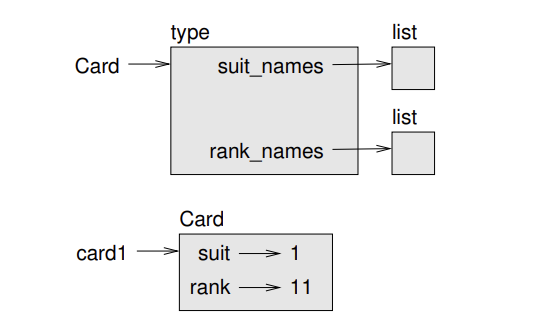
\includegraphics[width=0.5\textwidth]{./images/chapter_18_1.png}
\caption{Diagrama de objeto.}
\label{fig:class_diagrama}
\end{figure}

Cada carta tiene su propio palo y rango, pero solo hay una copia de \texttt{nombres\_palos} y \texttt{nombres\_rangos}.

Juntando todo, la expresión \texttt{Carta.nombres\_rangos[self.rango]} significa "usa el atributo \texttt{rango} del objeto \texttt{self} como un índice en la lista \texttt{nombres\_rangos} de la clase \texttt{Carta}, y selecciona la cadena apropiada."

El primer elemento de \texttt{nombres\_rangos} es \texttt{None} porque no hay una carta con rango cero. Al incluir \texttt{None} como marcador de posición, obtenemos un mapeo con la propiedad agradable de que el índice 2 se asigna a la cadena '2', y así sucesivamente. Para evitar este ajuste, podríamos haber usado un diccionario en lugar de una lista.

Con los métodos que tenemos hasta ahora, podemos crear e imprimir cartas:

\begin{lstlisting}[language=Python]
>>> carta1 = Carta(2, 11)
>>> print(carta1)
Jota de Corazones
\end{lstlisting}

La Figura 18.1 es un diagrama de la clase \texttt{Carta} y una instancia de \texttt{Carta}. \texttt{Carta} es un objeto clase; su tipo es \texttt{type}. \texttt{carta1} es una instancia de \texttt{Carta}, por lo que su tipo es \texttt{Carta}. Para ahorrar espacio, no dibujé el contenido de \texttt{nombres\_palos} y \texttt{nombres\_rangos}.

\section{Comparando cartas}

Para tipos integrados, hay operadores relacionales (<, >, ==, etc.) que comparan valores y determinan cuándo uno es mayor que, menor que o igual a otro. Para tipos definidos por el programador, podemos anular el comportamiento de los operadores integrados proporcionando un método llamado \texttt{\_\_lt\_\_}, que significa "menor que".

\texttt{\_\_lt\_\_} toma dos parámetros, \texttt{self} y \texttt{other}, y devuelve \texttt{True} si \texttt{self} es estrictamente menor que \texttt{other}.

El orden correcto para las cartas no es obvio. Por ejemplo, ¿cuál es mejor, el 3 de Tréboles o el 2 de Diamantes? Uno tiene un rango más alto, pero el otro tiene un palo más alto. Para comparar cartas, tienes que decidir si el rango o el palo es más importante.

La respuesta podría depender del juego que estés jugando, pero para mantener las cosas simples, haremos la elección arbitraria de que el palo es más importante, por lo que todas las Picas superan a todos los Diamantes, y así sucesivamente.

Con eso decidido, podemos escribir \texttt{\_\_lt\_\_}:

\begin{lstlisting}[language=Python]
# dentro de la clase Carta:

def __lt__(self, other):
    # verificar los palos
    if self.palo < other.palo: return True
    if self.palo > other.palo: return False

    # los palos son iguales... verificar los rangos
    return self.rango < other.rango
\end{lstlisting}

Puedes escribir esto de manera más concisa usando comparación de tuplas:

\begin{lstlisting}[language=Python]
# dentro de la clase Carta:

def __lt__(self, other):
    t1 = self.palo, self.rango
    t2 = other.palo, other.rango
    return t1 < t2
\end{lstlisting}

Como ejercicio, escribe un método \texttt{\_\_lt\_\_} para objetos \texttt{Tiempo}. Puedes usar comparación de tuplas, pero también podrías considerar comparar enteros.

\section{Mazos}

Ahora que tenemos \texttt{Cartas}, el siguiente paso es definir \texttt{Mazos}. Como un mazo está compuesto de cartas, es natural que cada \texttt{Mazo} contenga una lista de cartas como atributo.

La siguiente es una definición de clase para \texttt{Mazo}. El método \texttt{\_\_init\_\_} crea el atributo \texttt{cartas} y genera el conjunto estándar de cincuenta y dos cartas:

\begin{lstlisting}[language=Python]
class Mazo:

    def __init__(self):
        self.cartas = []
        for palo in range(4):
            for rango in range(1, 14):
                carta = Carta(palo, rango)
                self.cartas.append(carta)
\end{lstlisting}

La forma más fácil de llenar el mazo es con un bucle anidado. El bucle externo enumera los palos de 0 a 3. El bucle interno enumera los rangos de 1 a 13. Cada iteración crea una nueva \texttt{Carta} con el palo y rango actual, y la agrega a \texttt{self.cartas}.

\section{Imprimiendo el mazo}

Aquí hay un método \texttt{\_\_str\_\_} para \texttt{Mazo}:

\begin{lstlisting}[language=Python]
# dentro de la clase Mazo:

def __str__(self):
    res = []
    for carta in self.cartas:
        res.append(str(carta))
    return '\n'.join(res)
\end{lstlisting}

Este método demuestra una forma eficiente de acumular una cadena larga: construyendo una lista de cadenas y luego usando el método de cadena \texttt{join}. La función integrada \texttt{str} invoca el método \texttt{\_\_str\_\_} en cada carta y devuelve la representación de cadena. Como invocamos \texttt{join} en un carácter de nueva línea, las cartas están separadas por saltos de línea. Así es como se ve el resultado:

\begin{lstlisting}[language=Python]
>>> mazo = Mazo()
>>> print(mazo)
As de Tréboles
2 de Tréboles
3 de Tréboles
...
10 de Picas
Jota de Picas
Reina de Picas
Rey de Picas
\end{lstlisting}

Aunque el resultado aparece en 52 líneas, es una cadena larga que contiene saltos de línea.

\section{Agregar, eliminar, barajar y ordenar}

Para repartir cartas, nos gustaría un método que elimine una carta del mazo y la devuelva. El método \texttt{pop} de lista proporciona una forma conveniente de hacer eso:

\begin{lstlisting}[language=Python]
# dentro de la clase Mazo:
def pop_carta(self):
    return self.cartas.pop()
\end{lstlisting}

Como \texttt{pop} elimina la \textit{última} carta de la lista, estamos repartiendo desde el fondo del mazo. Para agregar una carta, podemos usar el método \texttt{append} de lista:

\begin{lstlisting}[language=Python]
# dentro de la clase Mazo:
def agregar_carta(self, carta):
    self.cartas.append(carta)
\end{lstlisting}

Un método como este que usa otro método sin hacer mucho trabajo a veces se llama \textbf{chapa}. La metáfora proviene de la carpintería, donde una chapa es una capa delgada de madera de buena calidad pegada a la superficie de una pieza más barata para mejorar la apariencia. En este caso, \texttt{agregar\_carta} es un método "delgado" que expresa una operación de lista en términos apropiados para mazos. Mejora la apariencia, o interfaz, de la implementación.

Como otro ejemplo, podemos escribir un método \texttt{barajar} para \texttt{Mazo} usando la función \texttt{shuffle} del módulo \texttt{random}:

\begin{lstlisting}[language=Python]
# dentro de la clase Mazo:
def barajar(self):
    random.shuffle(self.cartas)
\end{lstlisting}

No olvides importar \texttt{random}.

Como ejercicio, escribe un método \texttt{ordenar} para \texttt{Mazo} que use el método \texttt{sort} de lista para ordenar las cartas en un \texttt{Mazo}. \texttt{sort} usa el método \texttt{\_\_lt\_\_} que definimos para determinar el orden.

\section{Herencia}

La herencia es la capacidad de definir una nueva clase que es una versión modificada de una clase existente. Como ejemplo, digamos que queremos una clase para representar una "mano", es decir, las cartas que sostiene un jugador. Una mano es similar a un mazo: ambos están compuestos por una colección de cartas, y ambos requieren operaciones como agregar y eliminar cartas.

Una mano también es diferente de un mazo; hay operaciones que queremos para manos que no tienen sentido para un mazo. Por ejemplo, en póker podríamos comparar dos manos para ver cuál gana. En bridge, podríamos calcular una puntuación para una mano con el fin de hacer una oferta.

Esta relación entre clases—similar, pero diferente—se presta a la herencia. Para definir una nueva clase que herede de una clase existente, pones el nombre de la clase existente entre paréntesis:

\begin{lstlisting}[language=Python]
class Mano(Mazo):
    """Representa una mano de cartas de juego."""
\end{lstlisting}

Esta definición indica que \texttt{Mano} hereda de \texttt{Mazo}; eso significa que podemos usar métodos como \texttt{pop\_carta} y \texttt{agregar\_carta} para \texttt{Manos} así como para \texttt{Mazos}.

Cuando una nueva clase hereda de una existente, la existente se llama \textbf{clase padre} y la nueva clase se llama \textbf{clase hija}.

En este ejemplo, \texttt{Mano} hereda \texttt{\_\_init\_\_} de \texttt{Mazo}, pero no hace exactamente lo que queremos: en lugar de llenar la mano con 52 cartas nuevas, el método \texttt{\_\_init\_\_} para \texttt{Manos} debería inicializar \texttt{cartas} con una lista vacía.

Si proporcionamos un método \texttt{\_\_init\_\_} en la clase \texttt{Mano}, anula el de la clase \texttt{Mazo}:

\begin{lstlisting}[language=Python]
# dentro de la clase Mano:

def __init__(self, etiqueta=''):
    self.cartas = []
    self.etiqueta = etiqueta
\end{lstlisting}

Cuando creas una \texttt{Mano}, Python invoca este método \texttt{\_\_init\_\_}, no el de \texttt{Mazo}.

\begin{lstlisting}[language=Python]
>>> mano = Mano('mano nueva')
>>> mano.cartas
[]
>>> mano.etiqueta
'mano nueva'
\end{lstlisting}

Los otros métodos se heredan de \texttt{Mazo}, por lo que podemos usar \texttt{pop\_carta} y \texttt{agregar\_carta} para repartir una carta:

\begin{lstlisting}[language=Python]
>>> mazo = Mazo()
>>> carta = mazo.pop_carta()
>>> mano.agregar_carta(carta)
>>> print(mano)
Rey de Picas
\end{lstlisting}


Un siguiente paso natural es encapsular este código en un método llamado \texttt{mover\_cartas}:

\begin{lstlisting}[language=Python]
# dentro de la clase Mazo:

def mover_cartas(self, mano, num):
    for i in range(num):
        mano.agregar_carta(self.pop_carta())
\end{lstlisting}

\texttt{mover\_cartas} toma dos argumentos, un objeto \texttt{Mano} y el número de cartas a repartir. Modifica tanto \texttt{self} como \texttt{mano}, y devuelve \texttt{None}.

En algunos juegos, las cartas se mueven de una mano a otra, o de una mano de vuelta al mazo. Puedes usar \texttt{mover\_cartas} para cualquiera de estas operaciones: \texttt{self} puede ser un \texttt{Mazo} o una \texttt{Mano}, y \texttt{mano}, a pesar del nombre, también puede ser un \texttt{Mazo}.

La herencia es una característica útil. Algunos programas que serían repetitivos sin herencia pueden escribirse de manera más elegante con ella. La herencia puede facilitar la reutilización de código, ya que puedes personalizar el comportamiento de las clases padre sin tener que modificarlas. En algunos casos, la estructura de herencia refleja la estructura natural del problema, lo que facilita el diseño.

Por otro lado, la herencia puede hacer que los programas sean difíciles de leer. Cuando se invoca un método, a veces no está claro dónde encontrar su definición. El código relevante puede estar distribuido en varios módulos. Además, muchas de las cosas que se pueden hacer con herencia también se pueden hacer igual o mejor sin ella.

\section{Diagramas de clase}

Hasta ahora hemos visto diagramas de pila, que muestran el estado de un programa, y diagramas de objetos, que muestran los atributos de un objeto y sus valores. Estos diagramas representan una instantánea en la ejecución de un programa, por lo que cambian a medida que el programa se ejecuta.

También son muy detallados; para algunos propósitos, demasiado detallados. Un diagrama de clase es una representación más abstracta de la estructura de un programa. En lugar de mostrar objetos individuales, muestra clases y las relaciones entre ellas.

Hay varios tipos de relaciones entre clases:

\begin{itemize}
    \item Los objetos en una clase pueden contener referencias a objetos en otra clase. Por ejemplo, cada \texttt{Rectángulo} contiene una referencia a un \texttt{Punto}, y cada \texttt{Mazo} contiene referencias a muchas \texttt{Cartas}. Este tipo de relación se llama \textbf{HAS-A}, como en "un Rectángulo tiene un Punto."
    \item Una clase podría heredar de otra. Esta relación se llama \textbf{IS-A}, como en "una Mano es un tipo de Mazo."
    \item Una clase podría depender de otra en el sentido de que los objetos en una clase toman objetos en la segunda clase como parámetros, o usan objetos en la segunda clase como parte de un cálculo. Este tipo de relación se llama \textbf{dependencia}.
\end{itemize}

Un \textbf{diagrama de clase} es una representación gráfica de estas relaciones. Por ejemplo, la Figura 18.2 muestra las relaciones entre \texttt{Carta}, \texttt{Mazo} y \texttt{Mano}.

\begin{figure}[h]
\centering
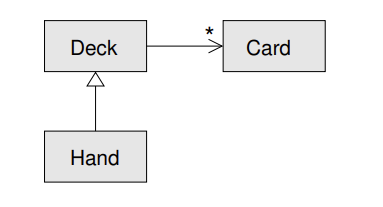
\includegraphics[width=0.5\textwidth]{./images/chapter_18_2.png}
\caption{Diagrama de clase.}
\label{fig:class_diagram}
\end{figure}

La flecha con una cabeza de triángulo hueco representa una relación IS-A; en este caso, indica que \texttt{Mano} hereda de \texttt{Mazo}.

La cabeza de flecha estándar representa una relación HAS-A; en este caso, un \texttt{Mazo} tiene referencias a objetos \texttt{Carta}.

El asterisco (*) cerca de la cabeza de la flecha es una multiplicidad; indica cuántas \texttt{Cartas} tiene un \texttt{Mazo}. Una multiplicidad puede ser un número simple, como 52, un rango, como 5..7, o un asterisco, que indica que un \texttt{Mazo} puede tener cualquier número de \texttt{Cartas}.

No hay dependencias en este diagrama. Normalmente se mostrarían con una flecha discontinua. O si hay muchas dependencias, a veces se omiten.

Un diagrama más detallado podría mostrar que un \texttt{Mazo} en realidad contiene una lista de \texttt{Cartas}, pero los tipos integrados como \texttt{list} y \texttt{dict} generalmente no se incluyen en los diagramas de clase.

\section{Depuración}

La herencia puede dificultar la depuración porque cuando invocas un método en un objeto, puede ser difícil averiguar qué método se invocará.

Supongamos que estás escribiendo una función que funciona con objetos \texttt{Mano}. Te gustaría que funcione con todo tipo de Manos, como \texttt{ManosDePóker}, \texttt{ManosDeBridge}, etc. Si invocas un método como \texttt{barajar}, podrías obtener el definido en \texttt{Mazo}, pero si alguna de las subclases anula este método, obtendrás esa versión en su lugar. Este comportamiento suele ser algo bueno, pero puede ser confuso.

Cada vez que no estés seguro del flujo de ejecución de tu programa, la solución más simple es agregar declaraciones de impresión al principio de los métodos relevantes. Si \texttt{Mazo.barajar} imprime un mensaje que dice algo como "Ejecutando \texttt{Mazo.barajar}", entonces, a medida que el programa se ejecuta, rastreará el flujo de ejecución.

Como alternativa, podrías usar esta función, que toma un objeto y un nombre de método (como una cadena) y devuelve la clase que proporciona la definición del método:

\begin{lstlisting}[language=Python]
def encontrar_clase_definidora(obj, nombre_metodo):
    for ty in type(obj).mro():
        if nombre_metodo in ty.__dict__:
            return ty
\end{lstlisting}

Aquí hay un ejemplo:

\begin{lstlisting}[language=Python]
>>> mano = Mano()
>>> encontrar_clase_definidora(mano, 'barajar')
<class '__main__.Mazo'>
\end{lstlisting}

Así que el método \texttt{barajar} para esta \texttt{Mano} es el de \texttt{Mazo}.

\texttt{encontrar\_clase\_definidora} usa el método \texttt{mro} para obtener la lista de objetos de clase (tipos) que se buscarán para los métodos. "MRO" significa "orden de resolución de método", que es la secuencia de clases que Python busca para "resolver" un nombre de método.

Aquí hay una sugerencia de diseño: cuando anulas un método, la interfaz del nuevo método debe ser la misma que la del antiguo. Debe tomar los mismos parámetros, devolver el mismo tipo y obedecer las mismas precondiciones y poscondiciones. Si sigues esta regla, encontrarás que cualquier función diseñada para trabajar con una instancia de una clase padre, como un \texttt{Mazo}, también funcionará con instancias de clases hijas como \texttt{Mano} y \texttt{ManoDePóker}.

Si violas esta regla, que se llama el "principio de sustitución de Liskov", tu código colapsará como (lo siento) un castillo de naipes.

\section{Encapsulamiento de datos}

Los capítulos anteriores demuestran un plan de desarrollo que podríamos llamar "diseño orientado a objetos". Identificamos los objetos que necesitábamos—como \texttt{Punto}, \texttt{Rectángulo} y \texttt{Tiempo}—y definimos clases para representarlos. En cada caso, hay una correspondencia obvia entre el objeto y alguna entidad en el mundo real (o al menos un mundo matemático).

Pero a veces es menos obvio qué objetos necesitas y cómo deberían interactuar. En ese caso, necesitas un plan de desarrollo diferente. De la misma manera que descubrimos interfaces de funciones mediante encapsulamiento y generalización, podemos descubrir interfaces de clases mediante \textbf{encapsulamiento de datos}.

El análisis de Markov, de la Sección 13.8, proporciona un buen ejemplo. Si descargas mi código de \url{https://thinkpython.com/code/markov.py}, verás que usa dos variables globales—\texttt{mapa\_sufijos} y \texttt{prefijo}—que se leen y escriben desde varias funciones.

\begin{lstlisting}[language=Python]
mapa_sufijos = {}
prefijo = ()
\end{lstlisting}

Debido a que estas variables son globales, solo podemos ejecutar un análisis a la vez. Si leemos dos textos, sus prefijos y sufijos se agregarían a las mismas estructuras de datos (lo que genera algunos textos generados interesantes).

Para ejecutar múltiples análisis y mantenerlos separados, podemos encapsular el estado de cada análisis en un objeto. Así es como se ve:

\begin{lstlisting}[language=Python]
class Markov:
    def __init__(self):
        self.mapa_sufijos = {}
        self.prefijo = ()
\end{lstlisting}

A continuación, transformamos las funciones en métodos. Por ejemplo, aquí está \texttt{procesar\_palabra}:

\begin{lstlisting}[language=Python]
def procesar_palabra(self, palabra, orden=2):
    if len(self.prefijo) < orden:
        self.prefijo += (palabra,)
        return

    try:
        self.mapa_sufijos[self.prefijo].append(palabra)
    except KeyError:
        # si no hay entrada para este prefijo, haz una
        self.mapa_sufijos[self.prefijo] = [palabra]
    self.prefijo = desplazar(self.prefijo, palabra)
\end{lstlisting}

Transformar un programa como este—cambiar el diseño sin cambiar el comportamiento—es otro ejemplo de refactorización (ver Sección 4.7).

Este ejemplo sugiere un plan de desarrollo para diseñar objetos y métodos:

\begin{enumerate}
    \item Comienza escribiendo funciones que lean y escriban variables globales (cuando sea necesario).
    \item Una vez que el programa funcione, busca asociaciones entre variables globales y las funciones que las usan.
    \item Encapsula las variables relacionadas como atributos de un objeto.
    \item Transforma las funciones asociadas en métodos de la nueva clase.
\end{enumerate}

Como ejercicio, descarga mi código Markov de \url{https://thinkpython.com/code/markov.py}, y sigue los pasos descritos anteriormente para encapsular las variables globales como atributos de una nueva clase llamada \texttt{Markov}. Solución: \url{https://thinkpython.com/code/markov2.py}.

\section{Glosario}

\begin{description}
    \item[codificar:] Representar un conjunto de valores usando otro conjunto de valores construyendo un mapeo entre ellos.
    \item[atributo de clase:] Un atributo asociado con un objeto de clase. Los atributos de clase se definen dentro de una definición de clase pero fuera de cualquier método.
    \item[atributo de instancia:] Un atributo asociado con una instancia de una clase.
    \item[chapa:] Un método o función que proporciona una interfaz diferente a otra función sin hacer mucho cálculo.
    \item[herencia:] La capacidad de definir una nueva clase que es una versión modificada de una clase previamente definida.
    \item[clase padre:] La clase desde la cual una clase hija hereda.
    \item[clase hija:] Una nueva clase creada heredando de una clase existente; también llamada "subclase".
    \item[relación IS-A:] Una relación entre una clase hija y su clase padre.
    \item[relación HAS-A:] Una relación entre dos clases donde las instancias de una clase contienen referencias a instancias de la otra.
    \item[dependencia:] Una relación entre dos clases donde las instancias de una clase usan instancias de la otra clase, pero no las almacenan como atributos.
    \item[diagrama de clase:] Un diagrama que muestra las clases en un programa y las relaciones entre ellas.
    \item[multiplicidad:] Una notación en un diagrama de clase que muestra, para una relación HAS-A, cuántas referencias hay a instancias de otra clase.
    \item[encapsulamiento de datos:] Un plan de desarrollo de programas que implica un prototipo que usa variables globales y una versión final que convierte las variables globales en atributos de instancia.
\end{description}

\section{Ejercicios}

\textbf{Ejercicio 18.1.} Para el siguiente programa, dibuja un diagrama de clases UML que muestre estas clases y las relaciones entre ellas.

\begin{lstlisting}[language=Python]
class PadrePingPong:
    pass

class Ping(PadrePingPong):
    def __init__(self, pong):
        self.pong = pong

class Pong(PadrePingPong):
    def __init__(self, pings=None):
        if pings is None:
            self.pings = []
        else:
            self.pings = pings

    def agregar_ping(self, ping):
        self.pings.append(ping)

pong = Pong()
ping = Ping(pong)
pong.agregar_ping(ping)
\end{lstlisting}

\textbf{Ejercicio 18.2.} Escribe un método de \texttt{Mazo} llamado \texttt{repartir\_manos} que tome dos parámetros, el número de manos y el número de cartas por mano. Debe crear el número apropiado de objetos \texttt{Mano}, repartir el número apropiado de cartas por mano y devolver una lista de \texttt{Manos}.

\textbf{Ejercicio 18.3.} Las siguientes son las posibles manos en póker, en orden creciente de valor y decreciente de probabilidad:

\begin{itemize}
    \item par: dos cartas con el mismo rango
    \item doble par: dos pares de cartas con el mismo rango
    \item tercia: tres cartas con el mismo rango
    \item escalera: cinco cartas con rangos en secuencia (los Ases pueden ser altos o bajos, por lo que As-2-3-4-5 es una escalera y también 10-Jota-Reina-Rey-As, pero Reina-Rey-As-2-3 no lo es)
    \item color: cinco cartas con el mismo palo
    \item full house: tres cartas con un rango, dos cartas con otro
    \item poker: cuatro cartas con el mismo rango
    \item escalera de color: cinco cartas en secuencia (como se definió anteriormente) y con el mismo palo
\end{itemize}

El objetivo de estos ejercicios es estimar la probabilidad de sacar estas varias manos.

\begin{enumerate}
    \item Descarga los siguientes archivos de \url{https://thinkpython.com/code}:
    \begin{itemize}
        \item \texttt{Card.py}: Una versión completa de las clases \texttt{Carta}, \texttt{Mazo} y \texttt{Mano} en este capítulo.
        \item \texttt{PokerHand.py}: Una implementación incompleta de una clase que representa una mano de póker, y algo de código que la prueba.
    \end{itemize}
    \item Si ejecutas \texttt{PokerHand.py}, reparte siete manos de póker de 7 cartas y verifica si alguna de ellas contiene un color. Lee este código cuidadosamente antes de continuar.
    \item Agrega métodos a \texttt{PokerHand.py} llamados \texttt{tiene\_par}, \texttt{tiene\_doble\_par}, etc. que devuelvan \texttt{True} o \texttt{False} según si la mano cumple o no con los criterios relevantes. Tu código debería funcionar correctamente para "manos" que contengan cualquier número de cartas (aunque 5 y 7 son los tamaños más comunes).
    \item Escribe un método llamado \texttt{clasificar} que determine la clasificación de mayor valor para una mano y establezca el atributo \texttt{etiqueta} en consecuencia. Por ejemplo, una mano de 7 cartas podría contener un color y un par; debería etiquetarse como "color".
    \item Cuando estés convencido de que tus métodos de clasificación funcionan, el siguiente paso es estimar las probabilidades de las varias manos. Escribe una función en \texttt{PokerHand.py} que baraje un mazo de cartas, lo divida en manos, clasifique las manos y cuente el número de veces que aparecen varias clasificaciones.
    \item Imprime una tabla de las clasificaciones y sus probabilidades. Ejecuta tu programa con números cada vez mayores de manos hasta que los valores de salida converjan a un grado razonable de precisión. Compara tus resultados con los valores en \url{http://en.wikipedia.org/wiki/Hand_rankings}.
\end{enumerate}

Solución: \url{https://thinkpython.com/code/PokerHandSoln.py}.
\chapter{Las bondades del lenguaje}

Uno de mis objetivos para este libro ha sido enseñarte la menor cantidad de Python posible. Cuando existían dos maneras de hacer algo, elegí una y evité mencionar la otra. O, a veces, coloqué la segunda opción en un ejercicio.

Ahora quiero retomar algunas de las características interesantes que dejamos de lado. Python ofrece varias funciones que no son realmente necesarias —puedes escribir buen código sin ellas—, pero con ellas a veces puedes escribir código más conciso, legible o eficiente... y en ocasiones, todo a la vez.

\section{Expresiones condicionales}

Vimos sentencias condicionales en la Sección 5.4. Las sentencias condicionales suelen usarse para elegir uno de dos valores; por ejemplo:

\begin{lstlisting}[language=Python]
if x > 0:
    y = math.log(x)
else:
    y = float('nan')
\end{lstlisting}

Esta sentencia verifica si \(x\) es positivo. Si lo es, se calcula \texttt{math.log}. En caso contrario, \texttt{math.log} generaría un \texttt{ValueError}. Para evitar que el programa se detenga, generamos un "NaN", que es un valor especial de punto flotante que representa "No es un número".

Podemos escribir esta sentencia de manera más concisa usando una \textbf{expresión condicional}:

\begin{lstlisting}[language=Python]
y = math.log(x) if x > 0 else float('nan')
\end{lstlisting}

Esta línea se puede leer casi como en inglés: "y obtiene log(x) si x es mayor que 0; en caso contrario obtiene NaN".

A veces, las funciones recursivas pueden reescribirse utilizando expresiones condicionales. Por ejemplo, aquí hay una versión recursiva de factorial:

\begin{lstlisting}[language=Python]
def factorial(n):
    if n == 0:
        return 1
    else:
        return n * factorial(n-1)
\end{lstlisting}

Podemos reescribirla así:

\begin{lstlisting}[language=Python]
def factorial(n):
    return 1 if n == 0 else n * factorial(n-1)
\end{lstlisting}

Otro uso de las expresiones condicionales es manejar argumentos opcionales. Por ejemplo, este es el método \texttt{init} de \texttt{GoodKangaroo} (ver Ejercicio 17.2):

\begin{lstlisting}[language=Python]
def __init__(self, name, contents=None):
    self.name = name
    if contents == None:
        contents = []
    self.pouch_contents = contents
\end{lstlisting}

Podemos reescribirlo así:

\begin{lstlisting}[language=Python]
def __init__(self, name, contents=None):
    self.name = name
    self.pouch_contents = [] if contents == None else contents
\end{lstlisting}

En general, puedes reemplazar una sentencia condicional con una expresión condicional si ambas ramas contienen expresiones simples que se asignan o se retornan a la misma variable.

\section{Comprensiones de listas}

En la Sección 10.7 vimos los patrones \texttt{map} y \texttt{filter}. Por ejemplo, esta función toma una lista de cadenas, aplica el método \texttt{capitalize} a cada elemento y retorna una nueva lista:

\begin{lstlisting}[language=Python]
def capitalize_all(t):
    res = []
    for s in t:
        res.append(s.capitalize())
    return res
\end{lstlisting}

Podemos escribir esto de forma más concisa usando una comprensión de lista:

\begin{lstlisting}[language=Python]
def capitalize_all(t):
    return [s.capitalize() for s in t]
\end{lstlisting}

Los corchetes indican que estamos construyendo una nueva lista. La expresión dentro de los corchetes especifica los elementos, y la cláusula \texttt{for} indica sobre qué secuencia iteramos.

Las comprensiones de listas también se pueden usar para filtrar. Por ejemplo, esta función selecciona solo los elementos de \texttt{t} que están en mayúscula y devuelve una nueva lista:

\begin{lstlisting}[language=Python]
def only_upper(t):
    res = []
    for s in t:
        if s.isupper():
            res.append(s)
    return res
\end{lstlisting}

\section{Expresiones generadoras}

Podemos reescribirla usando una comprensión de lista:

\begin{lstlisting}[language=Python]
def only_upper(t):
    return [s for s in t if s.isupper()]
\end{lstlisting}

Las comprensiones de listas son concisas y fáciles de leer, al menos para expresiones simples. Y suelen ser más rápidas que los bucles \texttt{for} equivalentes, a veces mucho más.

Las \textbf{expresiones generadoras} son similares, pero usan paréntesis en lugar de corchetes:

\begin{lstlisting}[language=Python]
>>> g = (x**2 for x in range(5))
>>> g
<generator object <genexpr> at 0x7f4c45a786c0>
\end{lstlisting}

El resultado es un objeto generador que sabe cómo iterar por una secuencia de valores. Pero, a diferencia de las comprensiones de lista, no calcula todos los valores de una vez; espera a que se le pidan. La función \texttt{next} obtiene el siguiente valor del generador:

\begin{lstlisting}[language=Python]
>>> next(g)
0
>>> next(g)
1
\end{lstlisting}

Cuando se alcanza el final de la secuencia, \texttt{next} lanza una excepción \texttt{StopIteration}. También puedes usar un bucle \texttt{for}:

\begin{lstlisting}[language=Python]
>>> for val in g:
...     print(val)
4
9
16
\end{lstlisting}

Las expresiones generadoras suelen usarse con funciones como \texttt{sum}, \texttt{max} y \texttt{min}:

\begin{lstlisting}[language=Python]
>>> sum(x**2 for x in range(5))
30
\end{lstlisting}

\section{\texttt{any} y \texttt{all}}

Python provee la función incorporada \texttt{any}, que toma una secuencia de valores booleanos y devuelve \texttt{True} si alguno es verdadero. Funciona con listas:

\begin{lstlisting}[language=Python]
>>> any([False, False, True])
True
\end{lstlisting}

Pero frecuentemente se usa con expresiones generadoras:

\begin{lstlisting}[language=Python]
>>> any(letter == 't' for letter in 'monty')
True
\end{lstlisting}

Podríamos usar \texttt{any} para reescribir algunas funciones de búsqueda de la Sección 9.3. Por ejemplo, podríamos escribir \texttt{avoids} así:

\begin{lstlisting}[language=Python]
def avoids(word, forbidden):
    return not any(letter in forbidden for letter in word)
\end{lstlisting}

Python también ofrece la función \texttt{all}, que retorna \texttt{True} si todos los elementos de la secuencia son verdaderos.

\section{Conjuntos (\texttt{sets})}

En la Sección 13.6 usamos diccionarios para encontrar palabras que aparecen en un documento pero no en una lista de palabras. La función escrita tomaba \texttt{d1} con palabras del documento como claves, y \texttt{d2} con la lista de palabras. Retornaba un diccionario con las claves de \texttt{d1} que no estaban en \texttt{d2}.

\begin{lstlisting}[language=Python]
def subtract(d1, d2):
    res = dict()
    for key in d1:
        if key not in d2:
            res[key] = None
    return res
\end{lstlisting}

Python ofrece otro tipo incorporado llamado \texttt{set}, que se comporta como una colección de claves sin valores. Podemos reescribir \texttt{subtract} así:

\begin{lstlisting}[language=Python]
def subtract(d1, d2):
    return set(d1) - set(d2)
\end{lstlisting}

Algunos ejercicios del libro pueden resolverse de forma más concisa y eficiente usando conjuntos. Por ejemplo, esta solución a \texttt{has\_duplicates} (Ejercicio 10.7) usando diccionarios:

\begin{lstlisting}[language=Python]
def has_duplicates(t):
    d = {}
    for x in t:
        if x in d:
            return True
        d[x] = True
    return False
\end{lstlisting}

Se puede reescribir con conjuntos así:

\begin{lstlisting}[language=Python]
def has_duplicates(t):
    return len(set(t)) < len(t)
\end{lstlisting}

También podemos usar conjuntos en ejercicios del Capítulo 9. Por ejemplo, una versión de \texttt{uses\_only} con bucles:

\begin{lstlisting}[language=Python]
def uses_only(word, available):
    for letter in word:
        if letter not in available:
            return False
    return True
\end{lstlisting}

Reescrita con conjuntos:

\begin{lstlisting}[language=Python]
def uses_only(word, available):
    return set(word) <= set(available)
\end{lstlisting}

\section{\texttt{Counter}}

Un \texttt{Counter} es como un conjunto, pero si un elemento aparece más de una vez, lleva la cuenta de cuántas veces aparece. Se encuentra en el módulo estándar \texttt{collections}, así que se debe importar:

\begin{lstlisting}[language=Python]
>>> from collections import Counter
>>> count = Counter('parrot')
>>> count
Counter({'r': 2, 't': 1, 'o': 1, 'p': 1, 'a': 1})
\end{lstlisting}

Podemos usar \texttt{Counter} para reescribir \texttt{is\_anagram} del Ejercicio 10.6:

\begin{lstlisting}[language=Python]
def is_anagram(word1, word2):
    return Counter(word1) == Counter(word2)
\end{lstlisting}

\section{\texttt{defaultdict}}

El módulo \texttt{collections} también provee \texttt{defaultdict}, que es como un diccionario, pero si accedes a una clave inexistente, puede generar un nuevo valor automáticamente.

\begin{lstlisting}[language=Python]
>>> from collections import defaultdict
>>> d = defaultdict(list)
>>> t = d['new key']
>>> t
[]
\end{lstlisting}

Esto permite evitar la creación de listas innecesarias y simplificar el código, como en este ejemplo:

\begin{lstlisting}[language=Python]
def all_anagrams(filename):
    d = defaultdict(list)
    for line in open(filename):
        word = line.strip().lower()
        t = signature(word)
        d[t].append(word)
    return d
\end{lstlisting}

\section{Tuplas con nombre}

Muchos objetos simples son básicamente colecciones de valores relacionados. Python ofrece una forma más concisa de representarlos:

\begin{lstlisting}[language=Python]
from collections import namedtuple
Point = namedtuple('Point', ['x', 'y'])
\end{lstlisting}

Para crear un objeto \texttt{Point}, se usa la clase como función:

\begin{lstlisting}[language=Python]
>>> p = Point(1, 2)
>>> p
Point(x=1, y=2)
\end{lstlisting}

\section{Recolección de argumentos nombrados}

En la Sección 12.4 vimos cómo definir una función que recolecta sus argumentos en una tupla:

\begin{lstlisting}[language=Python]
def printall(*args):
    print(args)
\end{lstlisting}

Para recolectar argumentos nombrados, puedes usar el operador \texttt{**}:

\begin{lstlisting}[language=Python]
def printall(*args, **kwargs):
    print(args, kwargs)
\end{lstlisting}

\section{Ejercicios}

\subsection*{Ejercicio 19.1}

La siguiente es una función que calcula el coeficiente binomial de manera recursiva.

\begin{lstlisting}[language=Python]
def binomial_coeff(n, k):
    """Calcula el coeficiente binomial "n sobre k".

    n: número de ensayos
    k: número de éxitos

    retorna: int
    """
    if k == 0:
        return 1
    if n == 0:
        return 0

    res = binomial_coeff(n-1, k) + binomial_coeff(n-1, k-1)
    return res
\end{lstlisting}

Reescribe el cuerpo de la función usando expresiones condicionales anidadas.

\appendix
\chapter{Depuración}

Cuando estás depurando, es importante distinguir entre diferentes tipos de errores para poder identificarlos más rápidamente:

\begin{itemize}
    \item \textbf{Errores de sintaxis}: Son detectados por el intérprete al traducir el código fuente a bytecode. Indican que hay algo mal en la estructura del programa. Ejemplo: Omitir los dos puntos al final de una sentencia \texttt{def} genera el mensaje \texttt{SyntaxError: invalid syntax}.
    
    \item \textbf{Errores en tiempo de ejecución}: Son producidos por el intérprete si algo sale mal mientras el programa se ejecuta. La mayoría de estos mensajes incluyen información sobre dónde ocurrió el error y qué funciones se estaban ejecutando. Ejemplo: Una recursión infinita causa el error \texttt{maximum recursion depth exceeded}.
    
    \item \textbf{Errores semánticos}: Son problemas en un programa que se ejecuta sin producir mensajes de error, pero no hace lo que debería. Ejemplo: Una expresión puede no evaluarse en el orden esperado, dando un resultado incorrecto.
\end{itemize}

El primer paso en la depuración es determinar qué tipo de error estás enfrentando. Aunque las siguientes secciones están organizadas por tipo de error, algunas técnicas son aplicables en más de una situación.

\section{Errores de sintaxis}

Los errores de sintaxis suelen ser fáciles de corregir una vez que los identificas. Desafortunadamente, los mensajes de error no siempre son útiles. Los más comunes son \texttt{SyntaxError: invalid syntax} y \texttt{SyntaxError: invalid token}, ninguno de los cuales es muy informativo.

Sin embargo, el mensaje sí te indica dónde ocurrió el problema en el programa. En realidad, te dice dónde Python notó el problema, que no necesariamente es donde está el error. A veces, el error está antes de la ubicación del mensaje, a menudo en la línea anterior.

Si estás construyendo el programa incrementalmente, deberías tener una idea clara de dónde está el error: estará en la última línea que agregaste.

Si estás copiando código de un libro, compara tu código con el del libro cuidadosamente. Revisa cada carácter. Al mismo tiempo, recuerda que el libro podría estar equivocado, así que si ves algo que parece un error de sintaxis, podría serlo.

Aquí hay algunas formas de evitar los errores de sintaxis más comunes:

\begin{enumerate}
    \item Asegúrate de no usar una palabra clave de Python como nombre de variable.
    \item Verifica que tengas dos puntos al final de cada encabezado de sentencia compuesta, como \texttt{for}, \texttt{while}, \texttt{if} y \texttt{def}.
    \item Asegúrate de que las cadenas en el código tengan comillas coincidentes y que sean comillas rectas (\texttt{"}), no curvas (\texttt{“}).
    \item Si tienes cadenas multilínea con comillas triples (simples o dobles), asegúrate de cerrarlas correctamente. Una cadena sin cerrar puede causar un error de token inválido al final del programa o tratar el siguiente código como parte de la cadena.
    \item Un operador de apertura sin cerrar (\texttt{(}, \texttt{\{}, \texttt{[}) hace que Python continúe con la siguiente línea como parte de la sentencia actual. Generalmente, el error ocurre casi inmediatamente en la siguiente línea.
    \item Revisa el clásico error de usar \texttt{=} en lugar de \texttt{==} en un condicional.
    \item Verifica la indentación para asegurarte de que esté alineada correctamente. Python puede manejar espacios y tabulaciones, pero mezclarlos puede causar problemas. La mejor forma de evitarlo es usar un editor de texto que reconozca Python y genere indentación consistente.
    \item Si tienes caracteres no ASCII en el código (incluyendo cadenas y comentarios), podrían causar problemas, aunque Python 3 generalmente los maneja. Ten cuidado al pegar texto de una página web u otra fuente.
\end{enumerate}

Si nada funciona, pasa a la siguiente sección...

\subsection{Sigo haciendo cambios y no hay diferencia.}

Si el intérprete dice que hay un error y no lo ves, podría ser porque tú y el intérprete no están viendo el mismo código. Verifica tu entorno de programación para asegurarte de que el programa que estás editando es el que Python está intentando ejecutar.

Si no estás seguro, intenta agregar un error de sintaxis obvio y deliberado al principio del programa. Ejecútalo de nuevo. Si el intérprete no encuentra el nuevo error, no estás ejecutando el código nuevo.

Algunas causas probables:

\begin{itemize}
    \item Editaste el archivo y olvidaste guardar los cambios antes de ejecutarlo de nuevo. Algunos entornos lo hacen por ti, pero otros no.
    \item Cambiaste el nombre del archivo, pero sigues ejecutando el nombre antiguo.
    \item Algo en tu entorno de desarrollo está configurado incorrectamente.
    \item Si estás escribiendo un módulo y usando \texttt{import}, asegúrate de no darle a tu módulo el mismo nombre que uno de los módulos estándar de Python.
    \item Si estás usando \texttt{import} para leer un módulo, recuerda que debes reiniciar el intérprete o usar \texttt{reload} para leer un archivo modificado. Si importas el módulo de nuevo, no hará nada.
\end{itemize}

Si estás atascado y no puedes entender qué pasa, un enfoque es comenzar de nuevo con un programa nuevo como "Hello, World!", y asegurarte de que puedes ejecutarlo. Luego, agrega gradualmente las partes del programa original al nuevo.

\section{Errores en tiempo de ejecución}

Una vez que tu programa es sintácticamente correcto, Python puede leerlo y al menos comenzar a ejecutarlo. ¿Qué podría salir mal?

\subsection{Mi programa no hace absolutamente nada.}

Este problema es común cuando tu archivo consiste en funciones y clases pero no invoca ninguna función para iniciar la ejecución. Esto puede ser intencional si solo planeas importar este módulo para usar sus clases y funciones.

Si no es intencional, asegúrate de que haya una llamada a función en el programa y de que el flujo de ejecución la alcance (ver "Flujo de ejecución" más adelante).

\subsection{Mi programa se cuelga.}

Si un programa se detiene y parece no hacer nada, está "colgado". A menudo, esto significa que está atrapado en un bucle infinito o una recursión infinita.

\begin{itemize}
    \item Si sospechas que un bucle en particular es el problema, agrega una sentencia \texttt{print} justo antes del bucle que diga "entrando al bucle" y otra justo después que diga "saliendo del bucle".
    \item Ejecuta el programa. Si obtienes el primer mensaje pero no el segundo, tienes un bucle infinito. Ve a la sección "Bucle infinito" más adelante.
    \item La mayoría de las veces, una recursión infinita hará que el programa se ejecute por un tiempo y luego produzca un error \texttt{RuntimeError: Maximum recursion depth exceeded}. Si eso pasa, ve a la sección "Recursión infinita".
    \item Si no obtienes este error pero sospechas que hay un problema con un método o función recursiva, aún puedes usar las técnicas de la sección "Recursión infinita".
    \item Si nada de eso funciona, prueba otros bucles y otras funciones o métodos recursivos.
    \item Si eso no funciona, es posible que no entiendas el flujo de ejecución de tu programa. Ve a la sección "Flujo de ejecución".
\end{itemize}

\subsubsection{Bucle infinito}

Si crees que tienes un bucle infinito y sabes qué bucle lo está causando, agrega una sentencia \texttt{print} al final del bucle que imprima los valores de las variables en la condición y el valor de la condición.

Por ejemplo:

\begin{lstlisting}[language=Python]
while x > 0 and y < 0:
    # hacer algo con x
    # hacer algo con y
    print('x:', x)
    print('y:', y)
    print("condición:", (x > 0 and y < 0))
\end{lstlisting}

Ahora, cuando ejecutes el programa, verás tres líneas de salida por cada iteración del bucle. La última vez que se ejecute el bucle, la condición debería ser \texttt{False}. Si el bucle sigue ejecutándose, podrás ver los valores de \texttt{x} e \texttt{y} y quizás descubrir por qué no se actualizan correctamente.

\subsubsection{Recursión infinita}

La mayoría de las veces, la recursión infinita hace que el programa se ejecute por un tiempo y luego produzca un error \texttt{Maximum recursion depth exceeded}.

Si sospechas que una función está causando una recursión infinita, asegúrate de que tenga un caso base. Debería haber alguna condición que haga que la función retorne sin invocarse recursivamente. Si no la hay, necesitas replantear el algoritmo e identificar un caso base.

Si hay un caso base pero el programa no parece alcanzarlo, agrega una sentencia \texttt{print} al inicio de la función que imprima los parámetros. Ahora, cuando ejecutes el programa, verás unas líneas de salida cada vez que la función se invoque, y podrás ver los valores de los parámetros. Si los parámetros no se acercan al caso base, obtendrás pistas sobre por qué.

\subsubsection{Flujo de ejecución}

Si no estás seguro de cómo se mueve el flujo de ejecución en tu programa, agrega sentencias \texttt{print} al inicio de cada función con un mensaje como "entrando a la función foo", donde \texttt{foo} es el nombre de la función.

Ahora, cuando ejecutes el programa, imprimirá un rastro de cada función a medida que se invoca.

\subsection{Cuando ejecuto el programa, obtengo una excepción.}

Si algo sale mal durante la ejecución, Python imprime un mensaje que incluye el nombre de la excepción, la línea del programa donde ocurrió el problema y un traceback.

El traceback identifica la función que se está ejecutando actualmente, luego la función que la llamó, y así sucesivamente. En otras palabras, traza la secuencia de llamadas a funciones que te llevaron al error, incluyendo el número de línea en tu archivo donde ocurrió cada llamada.

El primer paso es examinar el lugar del programa donde ocurrió el error y ver si puedes entender qué pasó. Estos son algunos de los errores en tiempo de ejecución más comunes:

\begin{itemize}
    \item \texttt{NameError}: Intentas usar una variable que no existe en el entorno actual. Revisa si el nombre está escrito correctamente, o al menos consistentemente. Recuerda que las variables locales son locales; no puedes referenciarlas desde fuera de la función donde están definidas.
    
    \item \texttt{TypeError}: Hay varias causas posibles:
    \begin{itemize}
        \item Intentas usar un valor de manera incorrecta. Ejemplo: indexar una cadena, lista o tupla con algo que no sea un entero.
        \item Hay una discrepancia entre los elementos en una cadena de formato y los elementos pasados para conversión. Esto puede pasar si el número de elementos no coincide o si se llama a una conversión inválida.
        \item Pasas el número incorrecto de argumentos a una función. Para métodos, revisa la definición del método y asegúrate de que el primer parámetro sea \texttt{self}. Luego revisa la invocación del método; asegúrate de que lo estás invocando en un objeto del tipo correcto y que estás pasando los demás argumentos correctamente.
    \end{itemize}
    
    \item \texttt{KeyError}: Intentas acceder a un elemento de un diccionario usando una clave que no contiene. Si las claves son cadenas, recuerda que las mayúsculas importan.
    
    \item \texttt{AttributeError}: Intentas acceder a un atributo o método que no existe. ¡Revisa la ortografía! Puedes usar la función incorporada \texttt{vars} para listar los atributos que sí existen.
    
    Si un \texttt{AttributeError} indica que un objeto es de tipo \texttt{NoneType}, significa que es \texttt{None}. Así que el problema no es el nombre del atributo, sino el objeto.
    
    La razón por la que el objeto es \texttt{None} podría ser que olvidaste retornar un valor de una función; si llegas al final de una función sin encontrar una sentencia \texttt{return}, retorna \texttt{None}. Otra causa común es usar el resultado de un método de lista, como \texttt{sort}, que retorna \texttt{None}.
    
    \item \texttt{IndexError}: El índice que usas para acceder a una lista, cadena o tupla es mayor que su longitud menos uno. Justo antes del lugar del error, agrega una sentencia \texttt{print} para mostrar el valor del índice y la longitud del arreglo. ¿El arreglo tiene el tamaño correcto? ¿El índice tiene el valor correcto?
\end{itemize}

El depurador de Python (\texttt{pdb}) es útil para rastrear excepciones porque te permite examinar el estado del programa justo antes del error. Puedes leer sobre \texttt{pdb} en \url{https://docs.python.org/3/library/pdb.html}.

\subsection{Agregué tantas sentencias print que me inundan con salida.}

Uno de los problemas de usar sentencias \texttt{print} para depurar es que puedes terminar enterrado en salida. Hay dos formas de proceder: simplificar la salida o simplificar el programa.

Para simplificar la salida, puedes eliminar o comentar las sentencias \texttt{print} que no estén ayudando, combinarlas o formatear la salida para que sea más fácil de entender.

Para simplificar el programa, hay varias cosas que puedes hacer. Primero, reduce el problema en el que está trabajando el programa. Por ejemplo, si estás buscando en una lista, busca en una lista pequeña. Si el programa recibe entrada del usuario, dale la entrada más simple que cause el problema.

Segundo, limpia el programa. Elimina código muerto y reorganízalo para hacerlo lo más legible posible. Por ejemplo, si sospechas que el problema está en una parte profundamente anidada del programa, intenta reescribir esa parte con una estructura más simple. Si sospechas de una función grande, intenta dividirla en funciones más pequeñas y probarlas por separado.

A menudo, el proceso de encontrar el caso de prueba mínimo te lleva al error. Si descubres que un programa funciona en una situación pero no en otra, eso te da una pista sobre lo que está pasando.

De manera similar, reescribir un fragmento de código puede ayudarte a encontrar errores sutiles. Si haces un cambio que crees que no debería afectar al programa, y lo hace, eso puede ser una señal.

\section{Errores semánticos}

En cierto modo, los errores semánticos son los más difíciles de depurar, porque el intérprete no proporciona información sobre lo que está mal. Solo tú sabes lo que se supone que debe hacer el programa.

El primer paso es hacer una conexión entre el texto del programa y el comportamiento que estás viendo. Necesitas una hipótesis sobre lo que el programa está haciendo realmente. Una de las cosas que lo hace difícil es que las computadoras son muy rápidas.

A menudo desearías poder ralentizar el programa a velocidad humana, y con algunos depuradores puedes hacerlo. Pero el tiempo que toma insertar algunas sentencias \texttt{print} bien colocadas suele ser corto comparado con configurar el depurador, insertar y eliminar puntos de interrupción, y "avanzar" el programa hasta donde ocurre el error.

\subsection{Mi programa no funciona.}

Debes hacerte estas preguntas:

\begin{itemize}
    \item ¿Hay algo que el programa debería hacer pero que no parece estar sucediendo? Encuentra la sección del código que realiza esa función y asegúrate de que se esté ejecutando cuando crees que debería.
    \item ¿Está sucediendo algo que no debería? Encuentra el código en tu programa que realiza esa función y verifica si se está ejecutando cuando no debería.
    \item ¿Una sección del código está produciendo un efecto que no es el esperado? Asegúrate de entender el código en cuestión, especialmente si involucra funciones o métodos de otros módulos de Python. Lee la documentación de las funciones que llamas. Pruébalas escribiendo casos de prueba simples y verificando los resultados.
\end{itemize}

Para programar, necesitas un modelo mental de cómo funcionan los programas. Si escribes un programa que no hace lo que esperas, a menudo el problema no está en el programa, sino en tu modelo mental.

La mejor manera de corregir tu modelo mental es dividir el programa en sus componentes (generalmente las funciones y métodos) y probar cada uno de manera independiente. Una vez que encuentres la discrepancia entre tu modelo y la realidad, podrás resolver el problema.

Por supuesto, deberías estar construyendo y probando componentes a medida que desarrollas el programa. Si encuentras un problema, solo debería haber una pequeña cantidad de código nuevo que no se sabe que sea correcto.

\subsection{Tengo una expresión enorme y no hace lo que espero.}

Escribir expresiones complejas está bien siempre que sean legibles, pero pueden ser difíciles de depurar. A menudo es una buena idea dividir una expresión compleja en una serie de asignaciones a variables temporales.

Por ejemplo:

\begin{lstlisting}[language=Python]
self.hands[i].addCard(self.hands[self.findNeighbor(i)].popCard())
\end{lstlisting}

Puede reescribirse como:

\begin{lstlisting}[language=Python]
neighbor = self.findNeighbor(i)
pickedCard = self.hands[neighbor].popCard()
self.hands[i].addCard(pickedCard)
\end{lstlisting}

La versión explícita es más fácil de leer porque los nombres de las variables proporcionan documentación adicional, y es más fácil de depurar porque puedes verificar los tipos de las variables intermedias y mostrar sus valores.

Otro problema que puede ocurrir con expresiones grandes es que el orden de evaluación puede no ser el que esperas. Por ejemplo, si estás traduciendo la expresión $\frac{x}{2\pi}$ a Python, podrías escribir:

\begin{lstlisting}[language=Python]
y = x / 2 * math.pi
\end{lstlisting}

Esto no es correcto porque la multiplicación y la división tienen la misma precedencia y se evalúan de izquierda a derecha. Así que esta expresión calcula $x\pi/2$.

Una buena manera de depurar expresiones es agregar paréntesis para hacer explícito el orden de evaluación:

\begin{lstlisting}[language=Python]
y = x / (2 * math.pi)
\end{lstlisting}

Siempre que no estés seguro del orden de evaluación, usa paréntesis. No solo el programa será correcto (en el sentido de hacer lo que pretendías), sino que también será más legible para otras personas que no hayan memorizado el orden de operaciones.

\subsection{Tengo una función que no retorna lo que espero.}

Si tienes una sentencia \texttt{return} con una expresión compleja, no tienes oportunidad de imprimir el resultado antes de retornar. Nuevamente, puedes usar una variable temporal. Por ejemplo, en lugar de:

\begin{lstlisting}[language=Python]
return self.hands[i].removeMatches()
\end{lstlisting}

Podrías escribir:

\begin{lstlisting}[language=Python]
count = self.hands[i].removeMatches()
return count
\end{lstlisting}

Ahora tienes la oportunidad de mostrar el valor de \texttt{count} antes de retornar.

\subsection{Estoy realmente, realmente atascado y necesito ayuda.}

Primero, intenta alejarte de la computadora por unos minutos. Las computadoras emiten ondas que afectan al cerebro, causando estos síntomas:

\begin{itemize}
    \item Frustración y enojo.
    \item Creencias supersticiosas ("la computadora me odia") y pensamiento mágico ("el programa solo funciona cuando uso mi gorra al revés").
    \item Programación aleatoria (el intento de programar escribiendo todos los programas posibles y eligiendo el que hace lo correcto).
\end{itemize}

Si te encuentras sufriendo alguno de estos síntomas, levántate y da un paseo. Cuando estés tranquilo, piensa en el programa. ¿Qué está haciendo? ¿Cuáles son algunas posibles causas de ese comportamiento? ¿Cuándo fue la última vez que tuviste un programa funcionando y qué hiciste después?

A veces, solo se necesita tiempo para encontrar un error. A menudo encuentro errores cuando estoy lejos de la computadora y dejo que mi mente divague. Algunos de los mejores lugares para encontrar errores son trenes, duchas y en la cama, justo antes de dormirte.

\subsection{No, realmente necesito ayuda.}

Sucede. Incluso los mejores programadores a veces se atascan. A veces trabajas en un programa tanto tiempo que no puedes ver el error. Necesitas una mirada fresca.

Antes de pedir ayuda, asegúrate de estar preparado. Tu programa debe ser lo más simple posible, y debes estar trabajando con la entrada más pequeña que causa el error. Debes tener sentencias \texttt{print} en los lugares apropiados (y su salida debe ser comprensible). Debes entender el problema lo suficiente como para describirlo de manera concisa.

Cuando pidas ayuda, asegúrate de dar la información necesaria:

\begin{itemize}
    \item Si hay un mensaje de error, ¿cuál es y qué parte del programa indica?
    \item ¿Qué fue lo último que hiciste antes de que ocurriera este error? ¿Cuáles fueron las últimas líneas de código que escribiste o cuál es el nuevo caso de prueba que falla?
    \item ¿Qué has intentado hasta ahora y qué has aprendido?
\end{itemize}

Cuando encuentres el error, tómate un segundo para pensar qué podrías haber hecho para encontrarlo más rápido. La próxima vez que veas algo similar, podrás encontrar el error más rápidamente.

Recuerda, el objetivo no es solo hacer que el programa funcione. El objetivo es aprender cómo hacer que el programa funcione.
\appendix

\chapter{Análisis de Algoritmos}

Este apéndice es un extracto editado de \textit{Think Complexity}, por Allen B. Downey, también publicado por O'Reilly Media (2012). Cuando termines con este libro, quizás quieras continuar con ese.

El \textbf{análisis de algoritmos} es una rama de la informática que estudia el rendimiento de los algoritmos, especialmente su tiempo de ejecución y requisitos de espacio. Ver \url{http://en.wikipedia.org/wiki/Analysis_of_algorithms}.

El objetivo práctico del análisis de algoritmos es predecir el rendimiento de diferentes algoritmos para guiar decisiones de diseño.

Durante la campaña presidencial de Estados Unidos en 2008, al candidato Barack Obama se le pidió que realizara un análisis improvisado cuando visitó Google. El director ejecutivo Eric Schmidt le preguntó en broma por "la forma más eficiente de ordenar un millón de enteros de 32 bits". Obama aparentemente había sido advertido, porque respondió rápidamente: "Creo que el ordenamiento de burbuja sería la forma incorrecta de hacerlo". Ver \url{http://www.youtube.com/watch?v=k4RRi_ntQc8}.

Esto es cierto: el ordenamiento de burbuja es conceptualmente simple pero lento para conjuntos de datos grandes. La respuesta que Schmidt probablemente buscaba es "ordenamiento por radix" (\url{http://en.wikipedia.org/wiki/Radix_sort})\footnote{Pero si te hacen una pregunta como esta en una entrevista, creo que una mejor respuesta es: "La forma más rápida de ordenar un millón de enteros es usar cualquier función de ordenamiento que proporcione el lenguaje que estoy usando. Su rendimiento es suficiente para la gran mayoría de las aplicaciones, pero si resultara que mi aplicación es demasiado lenta, usaría un perfilador para ver dónde se está gastando el tiempo. Si pareciera que un algoritmo de ordenamiento más rápido tendría un efecto significativo en el rendimiento, entonces buscaría una buena implementación del ordenamiento por radix."}.

El objetivo del análisis de algoritmos es hacer comparaciones significativas entre algoritmos, pero hay algunos problemas:

\begin{itemize}
    \item El rendimiento relativo de los algoritmos puede depender de las características del hardware, por lo que un algoritmo podría ser más rápido en la Máquina A y otro en la Máquina B. La solución general a este problema es especificar un \textbf{modelo de máquina} y analizar el número de pasos, u operaciones, que un algoritmo requiere bajo un modelo dado.
    
    \item El rendimiento relativo puede depender de los detalles del conjunto de datos. Por ejemplo, algunos algoritmos de ordenamiento se ejecutan más rápido si los datos ya están parcialmente ordenados; otros algoritmos se ejecutan más lento en este caso. Una forma común de evitar este problema es analizar el \textbf{peor caso}. A veces es útil analizar el rendimiento del caso promedio, pero eso suele ser más difícil y no siempre es obvio sobre qué conjunto de casos promediar.
    
    \item El rendimiento relativo también depende del tamaño del problema. Un algoritmo de ordenamiento que es rápido para listas pequeñas puede ser lento para listas largas. La solución habitual a este problema es expresar el tiempo de ejecución (o el número de operaciones) como una función del tamaño del problema, y agrupar las funciones en categorías dependiendo de qué tan rápido crecen a medida que aumenta el tamaño del problema.
\end{itemize}

Lo bueno de este tipo de comparación es que permite una clasificación simple de los algoritmos. Por ejemplo, si sé que el tiempo de ejecución del Algoritmo A tiende a ser proporcional al tamaño de la entrada, \( n \), y el Algoritmo B tiende a ser proporcional a \( n^2 \), entonces espero que A sea más rápido que B, al menos para valores grandes de \( n \).

Este tipo de análisis viene con algunas advertencias, pero las veremos más adelante.

\section{Orden de crecimiento}

Supongamos que has analizado dos algoritmos y has expresado sus tiempos de ejecución en términos del tamaño de la entrada: el Algoritmo A toma \( 100n + 1 \) pasos para resolver un problema de tamaño \( n \); el Algoritmo B toma \( n^2 + n + 1 \) pasos.

La siguiente tabla muestra el tiempo de ejecución de estos algoritmos para diferentes tamaños de problema:

\begin{center}
\begin{tabular}{|c|c|c|}
\hline
Tamaño de entrada & Tiempo de Algoritmo A & Tiempo de Algoritmo B \\
\hline
10 & 1,001 & 111 \\
100 & 10,001 & 10,101 \\
1,000 & 100,001 & 1,001,001 \\
10,000 & 1,000,001 & 100,010,001 \\
\hline
\end{tabular}
\end{center}

Para \( n = 10 \), el Algoritmo A se ve bastante mal; tarda casi 10 veces más que el Algoritmo B. Pero para \( n = 100 \) son aproximadamente iguales, y para valores más grandes, A es mucho mejor.

La razón fundamental es que para valores grandes de \( n \), cualquier función que contenga un término \( n^2 \) crecerá más rápido que una función cuyo término principal es \( n \). El \textbf{término principal} es el término con el exponente más alto.

Para el Algoritmo A, el término principal tiene un coeficiente grande, 100, por lo que B funciona mejor que A para \( n \) pequeños. Pero independientemente de los coeficientes, siempre habrá algún valor de \( n \) donde \( an^2 > bn \), para cualquier valor de \( a \) y \( b \).

El mismo argumento se aplica a los términos no principales. Incluso si el tiempo de ejecución del Algoritmo A fuera \( n + 1,000,000 \), seguiría siendo mejor que el Algoritmo B para \( n \) suficientemente grande.

En general, esperamos que un algoritmo con un término principal más pequeño sea un mejor algoritmo para problemas grandes, pero para problemas pequeños, puede haber un \textbf{punto de cruce} donde otro algoritmo es mejor. La ubicación del punto de cruce depende de los detalles de los algoritmos, las entradas y el hardware, por lo que generalmente se ignora para fines de análisis algorítmico. Pero eso no significa que puedas olvidarte de él.

\section{Orden de crecimiento}

Si dos algoritmos tienen el mismo término principal, es difícil decir cuál es mejor; nuevamente, la respuesta depende de los detalles. Por lo tanto, para el análisis algorítmico, las funciones con el mismo término principal se consideran equivalentes, incluso si tienen coeficientes diferentes.

Un \textbf{orden de crecimiento} es un conjunto de funciones cuyo comportamiento de crecimiento se considera equivalente. Por ejemplo, \( 2n \), \( 100n \) y \( n + 1 \) pertenecen al mismo orden de crecimiento, que se escribe \( O(n) \) en \textbf{notación Big-Oh} y a menudo se llama \textbf{lineal} porque cada función en el conjunto crece linealmente con \( n \).

Todas las funciones con el término principal \( n^2 \) pertenecen a \( O(n^2) \); se llaman \textbf{cuadráticas}.

La siguiente tabla muestra algunos de los órdenes de crecimiento que aparecen más comúnmente en el análisis algorítmico, en orden creciente de complejidad.

\begin{center}
\begin{tabular}{|c|c|}
\hline
Orden de crecimiento & Nombre \\
\hline
\( O(1) \) & constante \\
\( O(\log_b n) \) & logarítmico (para cualquier \( b \)) \\
\( O(n) \) & lineal \\
\( O(n \log_b n) \) & linearithmico \\
\( O(n^2) \) & cuadrático \\
\( O(n^3) \) & cúbico \\
\( O(c^n) \) & exponencial (para cualquier \( c \)) \\
\hline
\end{tabular}
\end{center}

Para los términos logarítmicos, la base del logaritmo no importa; cambiar de base es equivalente a multiplicar por una constante, lo que no cambia el orden de crecimiento. De manera similar, todas las funciones exponenciales pertenecen al mismo orden de crecimiento independientemente de la base del exponente. Las funciones exponenciales crecen muy rápidamente, por lo que los algoritmos exponenciales solo son útiles para problemas pequeños.

\begin{exercise}
Lee la página de Wikipedia sobre la notación Big-Oh en \url{http://en.wikipedia.org/wiki/Big_O_notation} y responde las siguientes preguntas:

\begin{enumerate}
    \item ¿Cuál es el orden de crecimiento de \( n^3 + n^2 \)? ¿Y de \( 1,000,000n^3 + n^2 \)? ¿Y de \( n^3 + 1,000,000n^2 \)?
    \item ¿Cuál es el orden de crecimiento de \( (n^2 + n) \cdot (n + 1) \)? Antes de empezar a multiplicar, recuerda que solo necesitas el término principal.
    \item Si \( f \) está en \( O(g) \), para alguna función no especificada \( g \), ¿qué podemos decir sobre \( af + b \), donde \( a \) y \( b \) son constantes?
    \item Si \( f_1 \) y \( f_2 \) están en \( O(g) \), ¿qué podemos decir sobre \( f_1 + f_2 \)?
    \item Si \( f_1 \) está en \( O(g) \) y \( f_2 \) está en \( O(h) \), ¿qué podemos decir sobre \( f_1 + f_2 \)?
    \item Si \( f_1 \) está en \( O(g) \) y \( f_2 \) está en \( O(h) \), ¿qué podemos decir sobre \( f_1 \cdot f_2 \)?
\end{enumerate}
\end{exercise}

Los programadores que se preocupan por el rendimiento a menudo encuentran este tipo de análisis difícil de digerir. Tienen un punto: a veces los coeficientes y los términos no principales marcan una diferencia real. A veces los detalles del hardware, el lenguaje de programación y las características de la entrada marcan una gran diferencia. Y para problemas pequeños, el orden de crecimiento es irrelevante.

Pero si tienes en cuenta estas advertencias, el análisis algorítmico es una herramienta útil. Al menos para problemas grandes, el algoritmo "mejor" suele ser mejor, y a veces es \textit{mucho} mejor. La diferencia entre dos algoritmos con el mismo orden de crecimiento suele ser un factor constante, pero la diferencia entre un buen algoritmo y un mal algoritmo no tiene límite.

\section{Análisis de operaciones básicas en Python}

En Python, la mayoría de las operaciones aritméticas son de tiempo constante; la multiplicación suele tardar más que la suma y la resta, y la división tarda aún más, pero estos tiempos de ejecución no dependen de la magnitud de los operandos. Los enteros muy grandes son una excepción; en ese caso, el tiempo de ejecución aumenta con el número de dígitos.

Las operaciones de indexación (leer o escribir elementos en una secuencia o diccionario) también son de tiempo constante, independientemente del tamaño de la estructura de datos.

Un bucle \texttt{for} que recorre una secuencia o diccionario suele ser lineal, siempre que todas las operaciones en el cuerpo del bucle sean de tiempo constante. Por ejemplo, sumar los elementos de una lista es lineal:

\begin{lstlisting}[language=Python]
total = 0
for x in t:
    total += x
\end{lstlisting}

La función incorporada \texttt{sum} también es lineal porque hace lo mismo, pero tiende a ser más rápida porque es una implementación más eficiente; en el lenguaje del análisis algorítmico, tiene un coeficiente principal más pequeño.

Como regla general, si el cuerpo de un bucle está en \( O(n^a) \), entonces todo el bucle está en \( O(n^{a+1}) \). La excepción es si puedes demostrar que el bucle termina después de un número constante de iteraciones. Si un bucle se ejecuta \( k \) veces independientemente de \( n \), entonces el bucle está en \( O(n^a) \), incluso para \( k \) grande.

Multiplicar por \( k \) no cambia el orden de crecimiento, pero tampoco dividir. Por lo tanto, si el cuerpo de un bucle está en \( O(n^a) \) y se ejecuta \( n/k \) veces, el bucle está en \( O(n^{a+1}) \), incluso para \( k \) grande.

La mayoría de las operaciones con cadenas y tuplas son lineales, excepto la indexación y \texttt{len}, que son de tiempo constante. Las funciones incorporadas \texttt{min} y \texttt{max} son lineales. El tiempo de ejecución de una operación de segmento es proporcional a la longitud de la salida, pero independiente del tamaño de la entrada.

La concatenación de cadenas es lineal; el tiempo de ejecución depende de la suma de las longitudes de los operandos.

Todos los métodos de cadenas son lineales, pero si las longitudes de las cadenas están limitadas por una constante (por ejemplo, operaciones en caracteres individuales), se consideran de tiempo constante. El método de cadena \texttt{join} es lineal; el tiempo de ejecución depende de la longitud total de las cadenas.

La mayoría de los métodos de listas son lineales, pero hay algunas excepciones:

\begin{itemize}
    \item Agregar un elemento al final de una lista es de tiempo constante en promedio; cuando se queda sin espacio, ocasionalmente se copia a una ubicación más grande, pero el tiempo total para \( n \) operaciones es \( O(n) \), por lo que el tiempo promedio para cada operación es \( O(1) \).
    \item Eliminar un elemento del final de una lista es de tiempo constante.
    \item Ordenar es \( O(n \log n) \).
\end{itemize}

La mayoría de las operaciones y métodos de diccionarios son de tiempo constante, pero hay algunas excepciones:

\begin{itemize}
    \item El tiempo de ejecución de \texttt{update} es proporcional al tamaño del diccionario pasado como parámetro, no al diccionario que se está actualizando.
    \item \texttt{keys}, \texttt{values} e \texttt{items} son de tiempo constante porque devuelven iteradores. Pero si iteras a través de los iteradores, el bucle será lineal.
\end{itemize}

\section{Análisis de algoritmos de búsqueda}

El rendimiento de los diccionarios es uno de los pequeños milagros de la informática. Veremos cómo funcionan en la Sección B.4.

\begin{exercise}
Lee la página de Wikipedia sobre algoritmos de ordenamiento en \url{http://en.wikipedia.org/wiki/Sorting_algorithm} y responde las siguientes preguntas:

\begin{enumerate}
    \item ¿Qué es un "ordenamiento por comparación"? ¿Cuál es el mejor orden de crecimiento en el peor caso para un ordenamiento por comparación? ¿Cuál es el mejor orden de crecimiento en el peor caso para cualquier algoritmo de ordenamiento?
    \item ¿Cuál es el orden de crecimiento del ordenamiento de burbuja y por qué Barack Obama cree que es "la forma incorrecta de hacerlo"?
    \item ¿Cuál es el orden de crecimiento del ordenamiento por radix? ¿Qué precondiciones necesitamos para usarlo?
    \item ¿Qué es un ordenamiento estable y por qué podría importar en la práctica?
    \item ¿Cuál es el peor algoritmo de ordenamiento (que tenga un nombre)?
    \item ¿Qué algoritmo de ordenamiento usa la biblioteca de C? ¿Qué algoritmo de ordenamiento usa Python? ¿Son estos algoritmos estables? Quizás tengas que buscar en Google para encontrar estas respuestas.
    \item Muchos de los ordenamientos que no son por comparación son lineales, entonces ¿por qué Python usa un ordenamiento por comparación \( O(n \log n) \)?
\end{enumerate}
\end{exercise}

\section{Algoritmos de búsqueda}

Una \textbf{búsqueda} es un algoritmo que toma una colección y un elemento objetivo y determina si el objetivo está en la colección, a menudo devolviendo el índice del objetivo.

El algoritmo de búsqueda más simple es una "búsqueda lineal", que recorre los elementos de la colección en orden, deteniéndose si encuentra el objetivo. En el peor caso, tiene que recorrer toda la colección, por lo que el tiempo de ejecución es lineal.

El operador \texttt{in} para secuencias usa una búsqueda lineal; lo mismo hacen los métodos de cadenas como \texttt{find} y \texttt{count}.

Si los elementos de la secuencia están ordenados, puedes usar una \textbf{búsqueda por bisección}, que es \( O(\log n) \). La búsqueda por bisección es similar al algoritmo que podrías usar para buscar una palabra en un diccionario (un diccionario de papel, no la estructura de datos). En lugar de comenzar al principio y revisar cada elemento en orden, comienzas con el elemento en el medio y verificas si la palabra que buscas viene antes o después. Si viene antes, buscas en la primera mitad de la secuencia. De lo contrario, buscas en la segunda mitad. De cualquier manera, reduces el número de elementos restantes a la mitad.

Si la secuencia tiene 1,000,000 de elementos, tomará unos 20 pasos encontrar la palabra o concluir que no está allí. Así que es unas 50,000 veces más rápido que una búsqueda lineal.

La búsqueda por bisección puede ser mucho más rápida que la búsqueda lineal, pero requiere que la secuencia esté ordenada, lo que podría requerir trabajo adicional.

Hay otra estructura de datos, llamada \textbf{tabla hash}, que es aún más rápida: puede hacer una búsqueda en tiempo constante, y no requiere que los elementos estén ordenados. Los diccionarios de Python se implementan usando tablas hash, por lo que la mayoría de las operaciones de diccionario, incluido el operador \texttt{in}, son de tiempo constante.

\section{Tablas hash}

Para explicar cómo funcionan las tablas hash y por qué su rendimiento es tan bueno, comenzaré con una implementación simple de un mapa y la mejoraré gradualmente hasta que sea una tabla hash.

Uso Python para demostrar estas implementaciones, pero en la vida real no escribirías código como este en Python; ¡simplemente usarías un diccionario! Así que por el resto de este capítulo, tienes que imaginar que los diccionarios no existen y que quieres implementar una estructura de datos que mapee claves a valores. Las operaciones que tienes que implementar son:

\begin{itemize}
    \item \texttt{add(k, v)}: Agrega un nuevo elemento que mapea la clave \( k \) al valor \( v \). Con un diccionario de Python, \( d \), esta operación se escribe \( d[k] = v \).
    \item \texttt{get(k)}: Busca y devuelve el valor que corresponde a la clave \( k \). Con un diccionario de Python, \( d \), esta operación se escribe \( d[k] \) o \( d.get(k) \).
\end{itemize}

Por ahora, asumiré que cada clave aparece solo una vez. La implementación más simple de esta interfaz utiliza una lista de tuplas, donde cada tupla es un par clave-valor.

\begin{lstlisting}[language=Python]
class LinearMap:
    def __init__(self):
        self.items = []
    
    def add(self, k, v):
        self.items.append((k, v))
    
    def get(self, k):
        for key, val in self.items:
            if key == k:
                return val
        raise KeyError
\end{lstlisting}

\texttt{add} agrega una tupla clave-valor a la lista de elementos, lo que toma tiempo constante.

\texttt{get} usa un bucle \texttt{for} para buscar en la lista: si encuentra la clave objetivo, devuelve el valor correspondiente; de lo contrario, genera un \texttt{KeyError}. Así que \texttt{get} es lineal.

Una alternativa es mantener la lista ordenada por clave. Entonces \texttt{get} podría usar una búsqueda por bisección, que es \( O(\log n) \). Pero insertar un nuevo elemento en medio de una lista es lineal, por lo que esta podría no ser la mejor opción. Hay otras estructuras de datos que pueden implementar \texttt{add} y \texttt{get} en tiempo logarítmico, pero eso sigue sin ser tan bueno como el tiempo constante, así que sigamos adelante.

Una forma de mejorar \texttt{LinearMap} es dividir la lista de pares clave-valor en listas más pequeñas. Aquí hay una implementación llamada \texttt{BetterMap}, que es una lista de 100 \texttt{LinearMaps}. Como veremos en un momento, el orden de crecimiento para \texttt{get} sigue siendo lineal, pero \texttt{BetterMap} es un paso hacia las tablas hash:

\begin{lstlisting}[language=Python]
class BetterMap:
    def __init__(self, n=100):
        self.maps = []
        for i in range(n):
            self.maps.append(LinearMap())
    
    def find_map(self, k):
        index = hash(k) % len(self.maps)
        return self.maps[index]
    
    def add(self, k, v):
        m = self.find_map(k)
        m.add(k, v)
    
    def get(self, k):
        m = self.find_map(k)
        return m.get(k)
\end{lstlisting}

\texttt{\_\_init\_\_} crea una lista de \( n \) \texttt{LinearMaps}.

\texttt{find\_map} es utilizado por \texttt{add} y \texttt{get} para determinar en qué mapa colocar el nuevo elemento o en qué mapa buscar.

\texttt{find\_map} usa la función incorporada \texttt{hash}, que toma casi cualquier objeto de Python y devuelve un entero. Una limitación de esta implementación es que solo funciona con claves hashables. Los tipos mutables como listas y diccionarios no son hashables.

Los objetos hashables que se consideran equivalentes devuelven el mismo valor hash, pero lo contrario no es necesariamente cierto: dos objetos con diferentes valores pueden devolver el mismo valor hash.

\texttt{find\_map} usa el operador módulo para ajustar los valores hash en el rango de 0 a \texttt{len(self.maps)}, por lo que el resultado es un índice válido en la lista. Por supuesto, esto significa que muchos valores hash diferentes se ajustarán al mismo índice. Pero si la función hash distribuye las cosas de manera bastante uniforme (que es lo que están diseñadas para hacer), esperamos \( n/100 \) elementos por \texttt{LinearMap}.

Dado que el tiempo de ejecución de \texttt{LinearMap.get} es proporcional al número de elementos, esperamos que \texttt{BetterMap} sea aproximadamente 100 veces más rápido que \texttt{LinearMap}. El orden de crecimiento sigue siendo lineal, pero el coeficiente principal es más pequeño. Eso es bueno, pero todavía no es tan bueno como una tabla hash.

Aquí está la idea crucial que hace que las tablas hash sean rápidas: si puedes mantener la longitud máxima de los \texttt{LinearMaps} acotada, \texttt{LinearMap.get} es de tiempo constante. Solo tienes que llevar un registro del número de elementos y, cuando el número de elementos por \texttt{LinearMap} supere un umbral, redimensionar la tabla hash agregando más \texttt{LinearMaps}.

Aquí hay una implementación de una tabla hash:

\begin{lstlisting}[language=Python]
class HashMap:
    def __init__(self):
        self.maps = BetterMap(2)
        self.num = 0
    
    def get(self, k):
        return self.maps.get(k)
    
    def add(self, k, v):
        if self.num == len(self.maps.maps):
            self.resize()
        
        self.maps.add(k, v)
        self.num += 1
    
    def resize(self):
        new_maps = BetterMap(self.num * 2)
        
        for m in self.maps.maps:
            for k, v in m.items:
                new_maps.add(k, v)
        
        self.maps = new_maps
\end{lstlisting}

\texttt{\_\_init\_\_} crea un \texttt{BetterMap} e inicializa \texttt{num}, que lleva un registro del número de elementos.

\texttt{get} simplemente delega a \texttt{BetterMap}. El trabajo real ocurre en \texttt{add}, que verifica el número de elementos y el tamaño del \texttt{BetterMap}: si son iguales, el número promedio de elementos por \texttt{LinearMap} es 1, por lo que llama a \texttt{resize}.

\texttt{resize} crea un nuevo \texttt{BetterMap}, el doble de grande que el anterior, y luego "rehashea" los elementos del mapa antiguo al nuevo.

El rehashing es necesario porque cambiar el número de \texttt{LinearMaps} cambia el denominador del operador módulo en \texttt{find\_map}. Eso significa que algunos objetos que solían hashear en el mismo \texttt{LinearMap} se dividirán (que es lo que queríamos, ¿verdad?).

El rehashing es lineal, por lo que \texttt{resize} es lineal, lo que podría parecer malo, ya que prometí que \texttt{add} sería de tiempo constante. Pero recuerda que no tenemos que redimensionar cada vez, por lo que \texttt{add} suele ser de tiempo constante y solo ocasionalmente lineal. La cantidad total de trabajo para ejecutar \texttt{add} \( n \) veces es proporcional a \( n \), por lo que el tiempo promedio de cada \texttt{add} es de tiempo constante.

Para ver cómo funciona esto, piensa en comenzar con un \texttt{HashTable} vacío y agregar una secuencia de elementos. Comenzamos con 2 \texttt{LinearMaps}, por lo que los primeros 2 \texttt{add} son rápidos (no se requiere redimensionamiento). Digamos que toman una unidad de trabajo cada uno. El siguiente \texttt{add} requiere un redimensionamiento, por lo que tenemos que rehashear los primeros dos elementos (digamos que son 2 unidades más de trabajo) y luego agregar el tercer elemento (una unidad más). Agregar el siguiente elemento cuesta 1 unidad, por lo que el total hasta ahora es de 6 unidades de trabajo para 4 elementos.

El siguiente \texttt{add} cuesta 5 unidades, pero los siguientes tres solo cuestan 1 unidad cada uno, por lo que el total es de 14 unidades para los primeros 8 \texttt{add}.

El siguiente \texttt{add} cuesta 9 unidades, pero luego podemos agregar 7 más antes del siguiente redimensionamiento, por lo que el total es de 30 unidades para los primeros 16 \texttt{add}.

Después de 32 \texttt{add}, el costo total es de 62 unidades, y espero que empieces a ver un patrón. Después de \( n \) \texttt{add}, donde \( n \) es una potencia de dos, el costo total es \( 2n - 2 \) unidades, por lo que el trabajo promedio por \texttt{add} es un poco menos de 2 unidades. Cuando \( n \) es una potencia de dos, ese es el mejor caso; para otros valores de \( n \), el trabajo promedio es un poco mayor, pero eso no es importante. Lo importante es que es \( O(1) \).

La Figura B.1 muestra cómo funciona esto gráficamente. Cada bloque representa una unidad de trabajo. Las columnas muestran el trabajo total para cada \texttt{add} en orden de izquierda a derecha: los primeros dos \texttt{add} cuestan 1 unidad cada uno, el tercero cuesta 3 unidades, etc.

El trabajo adicional de rehashing aparece como una secuencia de torres cada vez más altas con un espacio creciente entre ellas. Si derribas las torres, distribuyendo el costo del redimensionamiento sobre todos los \texttt{add}, puedes ver gráficamente que el costo total después de \( n \) \texttt{add} es \( 2n - 2 \).

Una característica importante de este algoritmo es que cuando redimensionamos el \texttt{HashTable}, crece geométricamente; es decir, multiplicamos el tamaño por una constante. Si aumentas el tamaño aritméticamente (agregando un número fijo cada vez), el tiempo promedio por \texttt{add} es lineal.

Puedes descargar mi implementación de \texttt{HashMap} desde \url{https://thinkpython.com/code/Map.py}, pero recuerda que no hay razón para usarla; si quieres un mapa, simplemente usa un diccionario de Python.

\section{Glosario}

\begin{description}
    \item[análisis de algoritmos:] Una forma de comparar algoritmos en términos de su tiempo de ejecución y/o requisitos de espacio.
    \item[modelo de máquina:] Una representación simplificada de una computadora utilizada para describir algoritmos.
    \item[peor caso:] La entrada que hace que un algoritmo dado se ejecute más lento (o requiera más espacio).
    \item[término principal:] En un polinomio, el término con el exponente más alto.
    \item[punto de cruce:] El tamaño del problema donde dos algoritmos requieren el mismo tiempo de ejecución o espacio.
    \item[orden de crecimiento:] Un conjunto de funciones que crecen de una manera considerada equivalente para fines de análisis de algoritmos. Por ejemplo, todas las funciones que crecen linealmente pertenecen al mismo orden de crecimiento.
    \item[notación Big-Oh:] Notación para representar un orden de crecimiento; por ejemplo, \( O(n) \) representa el conjunto de funciones que crecen linealmente.
    \item[lineal:] Un algoritmo cuyo tiempo de ejecución es proporcional al tamaño del problema, al menos para tamaños de problema grandes.
    \item[cuadrático:] Un algoritmo cuyo tiempo de ejecución es proporcional a \( n^2 \), donde \( n \) es una medida del tamaño del problema.
    \item[búsqueda:] El problema de localizar un elemento de una colección (como una lista o diccionario) o determinar que no está presente.
    \item[tabla hash:] Una estructura de datos que representa una colección de pares clave-valor y realiza búsquedas en tiempo constante.
\end{description}
\chapter{Índice}

Este capítulo contiene el índice completo del libro "Think Python 2", que sirve como referencia rápida para los términos y conceptos clave cubiertos en el texto.

\section{Índice alfabético}

\begin{description}
\item[abecedarian] 73, 84
\item[abs function] 52
\item[absolute path] 139, 145
\item[access] 90
\item[accumulator] 100
  \begin{itemize}
  \item histogram 127
  \item list 93
  \item string 175
  \item sum 93
  \end{itemize}
\item[Ackermann function] 61, 113
\item[add method] 165
\item[addition with carrying] 68
\item[algorithm] 67, 69, 130, 201
  \begin{itemize}
  \item MD5 146
  \item square root 69
  \end{itemize}
\item[aliasing] 95, 96, 100, 149, 151, 170
  \begin{itemize}
  \item copying to avoid 99
  \end{itemize}
\item[all] 186
\item[alphabet] 37
\item[alternative execution] 41
\item[ambiguity] 5
\item[anagram] 101
\item[anagram set] 123, 145
\item[analysis of algorithms] 201, 209
\item[analysis of primitives] 204
\item[and operator] 40
\item[any] 185
\item[append method] 92, 97, 101, 174, 175
\item[arc function] 31
\item[Archimedian spiral] 38
\item[argument] 17, 19, 21, 22, 26, 97
  \begin{itemize}
  \item gather 118
  \item keyword 33, 36, 191
  \item list 97
  \item optional 76, 79, 95, 107, 184
  \item positional 164, 169, 190
  \item variable-length tuple 118
  \end{itemize}
\item[argument scatter] 118
\item[arithmetic operator] 3
\item[assert statement] 159, 160
\item[assignment] 14, 63, 89
  \begin{itemize}
  \item augmented 93, 100
  \item item 74, 90, 116
  \item tuple 116, 117, 119, 122
  \end{itemize}
\item[assignment statement] 9
\item[attribute] 153, 169
  \begin{itemize}
  \item \_\_dict\_\_ 168
  \item class 172, 180
  \item initializing 168
  \item instance 148, 153, 172, 180
  \end{itemize}
\item[AttributeError] 152, 197
\item[augmented assignment] 93, 100
\item[Austen, Jane] 127
\item[average case] 202
\item[average cost] 208
\end{description}

\section{Ejemplos de código}

Aquí hay algunos ejemplos de código relevantes para términos del índice:

\begin{lstlisting}[language=Python]
# Ejemplo de función abs
x = -5
absolute_value = abs(x)
print(absolute_value)  # Output: 5

# Ejemplo de método append
my_list = [1, 2, 3]
my_list.append(4)
print(my_list)  # Output: [1, 2, 3, 4]

# Ejemplo de assert statement
def calculate_average(numbers):
    assert len(numbers) > 0, "List cannot be empty"
    return sum(numbers) / len(numbers)
\end{lstlisting}

\begin{lstlisting}[language=Python]
# Ejemplo de aliasing
a = [1, 2, 3]
b = a       # b es un alias de a
b[0] = 5    # Esto modifica tanto a como b
print(a)    # Output: [5, 2, 3]

# Para evitar aliasing
a = [1, 2, 3]
b = a.copy()  # b es una copia independiente
b[0] = 5     # Esto solo modifica b
print(a)     # Output: [1, 2, 3]
\end{lstlisting}

\section{Notas importantes}

El índice proporciona referencias cruzadas para todos los conceptos importantes cubiertos en el libro, incluyendo:

\begin{itemize}
\item Funciones incorporadas de Python
\item Métodos comunes
\item Conceptos de programación
\item Estructuras de datos
\item Técnicas de depuración
\item Diseño de algoritmos
\item Programación orientada a objetos
\end{itemize}

Para cada término, el número de página indica dónde encontrar la explicación detallada en el libro. Algunos términos tienen múltiples referencias cuando el concepto se discute en diferentes contextos a lo largo del texto.

\backmatter
% Bibliografía u otros anexos si fuera necesario

%\chapter*{Referencias}
%\bibliographystyle{apalike}
%\bibliography{referencias}

\end{document}